%%%%%%%%%%%%%%%%%%%%%%% file template.tex %%%%%%%%%%%%%%%%%%%%%%%%%
%
% This is a general template file for the LaTeX package SVJour3
% for Springer journals.          Springer Heidelberg 2010/09/16
%
% Copy it to a new file with a new name and use it as the basis
% for your article. Delete % signs as needed.
%
% This template includes a few options for different layouts and
% content for various journals. Please consult a previous issue of
% your journal as needed.
%
%%%%%%%%%%%%%%%%%%%%%%%%%%%%%%%%%%%%%%%%%%%%%%%%%%%%%%%%%%%%%%%%%%%
%
% First comes an example EPS file -- just ignore it and
% proceed on the \documentclass line
% your LaTeX will extract the file if required
%% \begin{filecontents*}{example.eps}
%% %!PS-Adobe-3.0 EPSF-3.0
%% %%BoundingBox: 19 19 221 221
%% %%CreationDate: Mon Sep 29 1997
%% %%Creator: programmed by hand (JK)
%% %%EndComments
%% gsave
%% newpath
%%   20 20 moveto
%%   20 220 lineto
%%   220 220 lineto
%%   220 20 lineto
%% closepath
%% 2 setlinewidth
%% gsave
%%   .4 setgray fill
%% grestore
%% stroke
%% grestore
%% \end{filecontents*}
%
\RequirePackage{fix-cm}
%
%\documentclass{svjour3}                     % onecolumn (standard format)
%\documentclass[smallcondensed]{svjour3}     % onecolumn (ditto)
%\documentclass[smallextended]{svjour3}       % onecolumn (second format)
\documentclass[twocolumn,final]{svjour3}          % twocolumn
%
\smartqed  % flush right qed marks, e.g. at end of proof
%
\usepackage{graphicx}
\usepackage{dblfloatfix}
\usepackage{soul}
\usepackage{natbib}
\usepackage{array}
\usepackage{colortbl}
\usepackage{bbm}
\usepackage{afterpage}
\newcolumntype{P}[1]{>{\centering\arraybackslash}p{#1}}
\usepackage{amsmath,amssymb} % define this before the line numbering.
%\usepackage{algorithm}
\usepackage{morefloats}
\usepackage{algorithm}
%\usepackage{morefloats}
\usepackage[noend]{algpseudocode}
%\usepackage{ruler}
%\usepackage{color}
%\usepackage[width=122mm,left=12mm,paperwidth=146mm,height=193mm,top=12mm,paperheight=217mm]{geometry}
\usepackage{mathrsfs}
\usepackage{url}
\usepackage{float}
\usepackage{subfigure}
%\usepackage{subfig}
\usepackage{multirow}
\usepackage{xcolor}
\usepackage{wrapfig}
\usepackage[toc,page]{appendix}
\usepackage[colorlinks]{hyperref}

\usepackage{mathtools}
\DeclarePairedDelimiter\ceil{\lceil}{\rceil}
\DeclarePairedDelimiter\floor{\lfloor}{\rfloor}

\def\G{{\cal G}}
\def\N{{\bf N}}
\def\T{{\bf T}}

\algnewcommand\algorithmicforeach{\textbf{for each}}
\algdef{S}[FOR]{ForEach}[1]{\algorithmicforeach\ #1\ \algorithmicdo}

\definecolor{orange}{RGB}{255,165,0}
\definecolor{purple}{RGB}{160,32,240}
\definecolor{brown}{RGB}{165,42,42}
\definecolor{gray}{RGB}{190,190,190}
\definecolor{cyan}{RGB}{0,255,255}
\definecolor{magenta}{RGB}{255,0,255}
\definecolor{deeppink}{RGB}{255,20,147}
\definecolor{tan}{RGB}{210,180,140}
\definecolor{darkorange}{RGB}{255,127,80}
\definecolor{darkgray}{RGB}{49,79,79}
\DeclareMathOperator*{\argmax}{arg\,max}
\DeclareRobustCommand\onedot{\futurelet\@let@token\@onedot}
\def\@onedot{\ifx\@let@token.\else.\null\fi\xspace}
\def\eg{\emph{e.g.}}
\def\Eg{\emph{E.g.}}
\def\ie{\emph{i.e.}}
\def\st{\emph{s.t.}}
\def\etc{\emph{etc.}}
\newcommand{\etal}{{\it et al. }}
%\newtheorem{definition}{Definition}
%\newtheorem{proposition}{Proposition}
%\newtheorem{mydef}{Definition}
\newcommand{\grad}{\nabla}
\newcommand{\RNum}[1]{\uppercase\expandafter{\romannumeral #1\relax}}
\newcommand{\rnum}[1]{\expandafter{\romannumeral #1\relax}}
\def\vs{\emph{vs}}
\def\FigureFont{\small}
\newcommand{\todo}{\textcolor{red}}
\urldef{\mailsa}\path|{yuliang_guo,maruthi_narayanan,benjamin_kimia}@brown.edu|


% correct bad hyphenation here
\hyphenation{op-tical net-works semi-conduc-tor}

\renewcommand{\cite}{\citep}
%
% \usepackage{mathptmx}      % use Times fonts if available on your TeX system
%
% insert here the call for the packages your document requires
%\usepackage{latexsym}
% etc.
%
% please place your own definitions here and don't use \def but
% \newcommand{}{}
%
% Insert the name of "your journal" with
% \journalname{myjournal}
%
\begin{document}

\title{Bottom-Up Perceptual Organization of Images into Object Part Proposals using Medial Visual Fragments}

%% \title{Insert your title here%\thanks{Grants or other notes
%% %about the article that should go on the front page should be
%% %placed here. General acknowledgments should be placed at the end of the article.}
%% }
%% \subtitle{Do you have a subtitle?\\ If so, write it here}

%% %\titlerunning{Short form of title}        % if too long for running head

\author{Maruthi Narayanan         \and
        Benjamin B. Kimia  %etc.
}

%\authorrunning{Short form of author list} % if too long for running head

\institute{F. Author \at
              first address \\
              Tel.: +123-45-678910\\
              Fax: +123-45-678910\\
              \email{fauthor@example.com}           %  \\
%             \emph{Present address:} of F. Author  %  if needed
           \and
           S. Author \at
              second address
}

\date{Received: date / Accepted: date}
% The correct dates will be entered by the editor


\maketitle

\begin{abstract}
The demise of ``segmentation-then-recognition'' strategy led to a paradigm shift
toward  feature-based discriminative recognition with significant success. However,  increased complexity in multi-class datasets reveals that local low-level
features may not be sufficiently discriminative, requiring the construction
and use of more complex structural features which are necessarily category independent. The paper proposes a bottom-up procedure for generating fragment features which are intended to be  {\em object part proposals}. Suggesting that the demise of segmentation to generate a representation suitable for recognition was due to prematurely committing to a grouping option in the face of ambiguities, the proposed framework considers and tracks multiple alternate grouping options. This approach is made tractable by \textit{(i)} using a \textit{medial fragment} representation which allows for the simultaneous use of multiple cues, \textit{(ii)} a set of transforms to effect grouping operations, \textit{(iii)}\ a  {\em containment graph} representation which avoids duplicate consideration of possibilities, and the estimation of the likelihood of a grouping sequence to retain only plausible groupings. The resulting hypotheses are evaluated intrinsically by measuring their ability to represent objects with a few fragments. They are also evaluated  by comparison to algorithms which aim to generate full object segments, with results that match or exceed the  state of art, thus   demonstrating the suitability of the proposed mid-level representation.

\keywords{First keyword \and Second keyword \and More}
% \PACS{PACS code1 \and PACS code2 \and more}
% \subclass{MSC code1 \and MSC code2 \and more}
\end{abstract}

\section{Introduction}
\label{sec:intro}

Object recognition, object detection, object tracking, object discovery, action recognition and other high-level visual tasks can benefit from an intermediate level representation that potentially represents objects or object parts. The act of identifying regions in the image that potentially correspond to objects is known as generating \emph{object proposals}~\cite{Malisiewicz:Efros:BMVC07, Alexe:etal:PAMI12, Endres:Hoiem:PAMI14, Carreira:Sminchisescu:PAMI12, Chang:etal:ICCV11, Rahtu:etal:ICCV11,Zhang:Torr:PAMI16, Feng:etal:ICCV11, Uijlings:etal:IJCV13, Narayanan:Kimia:ECCV12, Kim:Grauman:ECCV12, Manen:etal:ICCV13, Humayun:etal:CVPR14, Arbelaez:etal:CVPR14, Rantalankila:etal:CVPR14, Krahenbuhl:Koltun:ECCV14, Bonev:Yuille:ECCV14, Zitnick:Dollar:ECCV14, Cheng:etal:CVPR14, Erhan:etal:CVPR14, Krahenbuhl:Koltun:CVPR15, Xiao:Lu:etal:CVPR15, Chen:etal:CVPR15, Lu:etal:ICCV15, Humayun:etal:ICCV15, He:Lau:ICCV15}. While the current paradigm of decomposing an image into a set of \emph{object proposals} is popular among many different computer vision tasks the evolution to this now accepted intermediate from originates from the difficulties faced with ``sliding-window'' approaches in object detection.

Until most recently, the most successful approaches to object detection have all utilized the well known, ``sliding window'' paradigm~\cite{Papageorgiou:Poggio:IJCV00,Viola:Jones:IJCV04,Felzenszwalb:PAMI:09} in which a learned classifier tests for the presence of an object in every sampled candidate image window. In a general object detection setting, the number of candidate windows tested must be performed over all possible object positions, scales, and aspect ratios. The linear complexity of ``sliding window'' approaches with respect to the size of this 4-dimensional search space,$(x,y,w,h)$, makes it difficult to efficiently search over all possible windows. Even if the number of candidate windows was minimal the exponential growth in dataset sizes has naturally forced classifiers to become more sophisticated at the expense of increased computational run-time to evaluate a single window. Given that it is intractable to exhaustively evaluate these more complex classifiers over millions or possibly billions of image windows researchers have developed heuristics to speed up the search, at the risk of possibly mislocating or missing objects altogether. While there have been more structured approaches such as Branch and Bound~\cite{Lampert:etal:PAMI09} that do no resort to these heuristics, all ``sliding window'' approaches are forced to make trade-off's between  detection quality and computational tractability.  Overcoming this trade-off was the major driving factor toward the research and development of \emph{object proposals}. 

\emph{Object proposal} methods overcome this trade-off by utilizing segmentation as a pre-processing step to generate a small of pool candidate regions (on the order of thousands) that are then passed into various classification algorithms. Reasoning with this reduced set of regions allows ``sliding window'' approaches to bypass the need for searching over the space of all candidate windows. While the idea of utilizing segmentation as a precursor to recognition is not a novel idea the difficulties faced with classic segmentation rendered this paradigm moot. Two major leaps in thinking essentially overcame the difficulties in traditional segmentation and are the basis for all \emph{object proposal} schemes. The first major leap in thinking was the Soup of Segments~\cite{Malisiewicz:Efros:BMVC07} work which argued that rather than generate a single segmentation we should generate a diversity of segmentations. By exploring multiple segmentations we increase the likelihood of finding objects that are perfectly segmented in one partitioning but erroneously merged or broken in other segmentations. The second major idea was first made in 2010 concurrently by three independent groups, {\bf Objectness}~\cite{Alexe:etal:PAMI12}, {\bf CPMC}~\cite{Carreira:Sminchisescu:PAMI12}, and {\bf Category Independent Proposals}~\cite{Endres:Hoiem:PAMI14}. The key observation was that if our goal in subsequent processing is object centric tasks (recognition, detection, \etc) why focus on exhaustively partitioning, , Figure~\ref{fig:diffs}\textcolor{red}{(a)}, every pixel into a unique region? Rather we should focus on directly generating a pool of \emph{proposals} (bounding box or free-form regions), Figure~\ref{fig:diffs}\textcolor{red}{(c,d)}, that are likely to capture \emph{objects} in the scene without providing a complete image segmentation. By relaxing the original segmentation formulation to only focus on object-like area's of the image coupled with exploring multiple possibly overlapping segments the problem becomes more forgiving and we have a much greater chance of generating good proposals. 

\begin{figure}[ht]
\centering
{\footnotesize\textit{a)}}\includegraphics[width=0.228\textwidth]{figs/three.jpg}
{\footnotesize\textit{b)}}\includegraphics[width=0.228\textwidth]{figs/out.png}
{\footnotesize\textit{c)}}\includegraphics[width=0.228\textwidth]{figs/giraffe_bbox.png}
{\footnotesize\textit{d)}}\includegraphics[width=0.228\textwidth]{figs/giraffe_ops.png}
\caption{a) Image and classical segmentation in b). We see the object proposal representation in c) and d).}
\label{fig:diffs}
\end{figure}

\begin{figure}[ht]
\centering
{\footnotesize\textit{a)}}\includegraphics[width=0.229\textwidth]{figs/all_frags_per_image_part1.png}
{\footnotesize\textit{b)}}\includegraphics[width=0.229\textwidth]{figs/all_frags_per_image_part2.png}
{\footnotesize\textit{c)}}\includegraphics[height=0.13\textheight]{figs/horse_occlude.png}
{\footnotesize\textit{d)}}\includegraphics[width=0.235\textwidth]{figs/horse_no_occlude.png}
\caption{Examples of various part based object proposals generated by our approach in (a) and (b). For clarity, proposals from the background and full-object proposals are not shown. In (c) only a portion of the horse is shown due to occlusion while in (d) the full horse is recoverable. To correlate the two we must be able to recover the portion, head, of the objects visible in both images. The head is in highlighted in cyan. }
\label{fig:part_ops}
\end{figure}

Our work is distinct in both its goal and approach. The primary application of object proposals has been in object detection. As such, approaches have focused on recovering full object proposals in a scene, \ie, the three giraffes in Figure~\ref{fig:diffs}\textcolor{red}{(a)}. Our primary goal, however, is to recover parts and their combinations, \ie, legs, heads, tails, legs plus body, head plus neck, \etc, Figure~\ref{fig:part_ops}\textcolor{red}{(a,b)}. Part-based object proposals have received considerable less attention in the object proposal literature. Our motivation for focusing on parts is that the problem is much more tractable than trying to recover full objects. Furthermore, the recovery of parts is important when trying to correlate object proposal across scenes with varying degrees of occlusion, Figure~\ref{fig:part_ops}\textcolor{red}{(c,d)}. 



%% {\bf One of the major contributions of our work is to show how our approach is flexible enough to recover part-based proposals along with full object proposals.} 


\begin{figure}[ht]
\centering
{\footnotesize\textit{a)}}\includegraphics[width=0.229\textwidth]{figs/piggies.png}
{\footnotesize\textit{b)}}\includegraphics[width=0.229\textwidth]{figs/piggies_cons.pdf}
{\footnotesize\textit{c)}}\includegraphics[width=0.229\textwidth]{figs/bear_head.png}
{\footnotesize\textit{d)}}\includegraphics[width=0.229\textwidth]{figs/bear_head_cons.pdf}
{\footnotesize\textit{e)}}\includegraphics[width=0.229\textwidth]{figs/horse_occluded.pdf}
\caption{Reasoning with a purely regional representation of (a) will lead to the two pigs being merged as the two pigs are roughly homogenous. (b) If we consider a contour representation of the objects we see that the presence of the internal \textcolor{cyan}{cyan} provides a clue to the delineation of the two pigs. In (c) we see how a purely regional representation could lead to the ears merging with the rest of the bear head, but the \textcolor{cyan}{contours} in (d) roughly fall along the part lines of the ear. (e) We observe how purely reasoning with contour cues does not merge the two horse parts} 
\label{fig:cons_vs_regions}
\end{figure}

The majority of object proposal approaches are based on revisiting region-based segmentation in the context of recovering object proposals. As such approaches have repurposed the same regional representations of an image, Region-Adjacency Graph (RAG) of pixels or superpixels, region hierarchies, \etc, for the recovery of object proposals. An implicit assumption of these representations is that objects in a scene are exclusively defined by their regional signature, cohesive areas of color and texture, and the recovery of object proposals is simply a manipulation of this underlying representation, \ie, merging pixels or superpixels, partitioning the graph using graph cuts, \etc. This ignores the contour signature, silhouette curves, objects leave behind in their projection onto an image. Observe that in Figure~\ref{fig:cons_vs_regions}\textcolor{red}{(a)} a purely regional representation of the image could lead to the two pigs being merged as the objects are roughly homogenous in appearance. If we consider the contour signature, Figure~\ref{fig:cons_vs_regions}\textcolor{red}{(b)}, observe that the silhouette of the pig head is recovered, highlighted in \textcolor{cyan}{cyan}, providing strong evidence for the separation of these regions. The role of contours is even more important in the recovery of parts. Figure~\ref{fig:cons_vs_regions}\textcolor{red}{(c)} shows a black bear of roughly uniform appearance. While a regional representation could lead to the ears, head, and body merging the contour signature, Figure~\ref{fig:cons_vs_regions}\textcolor{red}{(d)} identifies internal contours, highlighted in \textcolor{cyan}{cyan}, falling along the part lines separating the head from the ear. While contour signatures are important regional signatures are still key. Observe in Figure~\ref{fig:cons_vs_regions}\textcolor{red}{(e)} the recovery of the full horse is occluded by the rider. While a contour representation can recover the two pieces, highlighted in cyan and magenta, the main cue to unify these two parts is the regional homogeneity. Finally, a more recent trend as proposed by~\cite{Bonev:Yuille:ECCV14} is to also recover contextual or background fragments, sky, grass, \etc. The recovery of these background proposals which lack any clear defined silhouette are better recovered by exclusively reasoning with the regional attributes. This is not just the old tale of integrating contours and regions, but rather the simultaneous representation of both. To do that we propose a new multi-faceted representation that captures both signatures in a unified fashion. 

%% {\bf One of the major contributions of our work is to propose a new multi-faceted representation that overcomes the limitations of current region and contour based representations.}

 
The second distinction between our approach and others is how we reason with our representation to generate object proposals. One of the key requirements of object proposals schemes is to achieve high recall, \ie, ALL objects in a scene should be recovered with sufficient quality. To satisfy this requirement a large pool of candidate proposals is generated with the assumption that if the pool is sufficiently large all objects in the scene will be recovered with high probability. Building off the Soup of Segments approach~\cite{Malisiewicz:Efros:BMVC07} this pool is generated by sweeping the parameters that govern that particular algorithm. In this view, each object proposal is generated by some combination of algorithm settings and the sweep of all possible parameters settings generates a set of possible object proposals. The difficulty of this approach is that there is no guarantee that objects will exactly map to some combination of parameters, and across datasets it is not clear how generalizable the parameter settings will be. 

\begin{figure*}[ht]
\centering
{\footnotesize\textit{a)}}\includegraphics[width=0.241\textwidth]{figs/ic_horses.pdf}
\includegraphics[width=0.241\textwidth]{figs/ic_kang.pdf}
\includegraphics[width=0.241\textwidth]{figs/ic_mush.pdf}
\includegraphics[width=0.241\textwidth]{figs/ic_car.pdf}
{\footnotesize\textit{b)}}\includegraphics[width=0.241\textwidth]{figs/rr_stripes.pdf}
\includegraphics[width=0.241\textwidth]{figs/rr_spots.pdf}
\includegraphics[width=0.241\textwidth]{figs/rr_markings.pdf}
\includegraphics[width=0.241\textwidth]{figs/rr_bus2.pdf}
{\footnotesize\textit{c)}}\includegraphics[width=0.241\textwidth]{figs/zebra_miss.pdf}
\includegraphics[width=0.241\textwidth]{figs/tiger_miss.pdf}
\includegraphics[width=0.241\textwidth]{figs/person_miss.pdf}
\includegraphics[height=0.16\textwidth]{figs/giraffe_miss.pdf}
{\footnotesize\textit{d)}}\includegraphics[width=0.243\textwidth]{figs/bear_segment.jpeg}
\includegraphics[width=0.243\textwidth]{figs/plane_segment.png}
\caption{We observe various examples of degradations to ideal signatures of objects in a scene. a) Despite ideal silhouettes, highlighted in red, \emph{clutter contours}, randomly colored, interrupt the recovery of the full object. b) Observe that \emph{clutter regions} interrupt the recovery of objects despite ideal silhouettes. c) The ideal silhouette is interrupted by \emph{contour gaps}. d) We see roughly homogenous objects disjointed into various regions that need to be merged to recover the whole. These results were illustrated with N-Cuts~\cite{Shi:Malik:PAMI00}, but the principle is the same irrespective of segmentation algorithm. } 
\label{fig:trans_examples}
\end{figure*}

In our work, we deviate drastically from this canonical view, and take a more structured approach where we look at the formation of object and part proposals as the process of recovering the ideal signatures (contour and region) given an image where object signatures have been degraded. Consider Figure~\ref{fig:trans_examples} where we see how the dual signatures of objects in a scene are distorted due to various imaging and scene affects. In Figure~\ref{fig:trans_examples}\textcolor{red}{(a,b)} we see how despite recovering an ideal contour silhouette, highlighted in red, the recovery of the full object and its parts is interrupted by the presence of \emph{contour-clutter} and \emph{region-clutter} respectively. For example, the muscles of the horse in Figure~\ref{fig:trans_examples}\textcolor{red}{(a)} lead to the formation of internal contours while the recovery of the people and bus in Figure~\ref{fig:trans_examples}\textcolor{red}{(b)} is interrupted by regional surface markings. In Figure~\ref{fig:trans_examples}\textcolor{red}{(c)} we we observe that even if we don't have any \emph{contour-clutter} or \emph{region-clutter} the ideal silhouette can be interrupted causing \emph{contour gaps} to form. Observe that the silhouettes of the zebra head, tiger head, and person are interrupted. And finally an ideal picture of a large homogenous region is unnecessarily disjointed due to scene and imaging effects disrupting the underlying appearance characteristics, Figure~\ref{fig:trans_examples}\textcolor{red}{(d)}. To recover the objects and parts in a scene we adopt a \emph{perceptual organization} approach where each of the degradations illustrated in Figure~\ref{fig:trans_examples} are dealt with in a Gestalt framework. For example, to recover the horse or person we must remove the clutter contours and clutter regions respectively, or we must complete gaps in the case of Figure~\ref{fig:trans_examples}\textcolor{red}{(d)} to recover the zebra head, tiger head, and human outline or finally some combination of these counter-actions is needed to recover more complex objects in a scene. This quickly leads to a large number of possibilities. These various grouping options are efficiently tracked and the entire set of options are maintained. This is an important distinction because while it is possible that viable fragments are not formed under the variations-of-variables scheme (\eg, object was too small and no seeds were initialized inside), it is much less likely that viable fragment would avoid being considered due to the structural and exhaustive nature of the proposed scheme. 

In summary, our main contributions are:

\begin{itemize}

\item A new multi-faceted representation that overcomes the limitations of current region and contour based representations (Section~\ref{sec:atomic:fragments}). 

\item The formalization of a new perceptual organization framework that maps high-level image degradations (presence of clutter, interruptions in contours, \etc) to a concrete set of contour-actions (transforms) (Section~\ref{sec:transforms}). 

\item An efficient strategy to practically explore the expansive and conflicting set of grouping options our Gestalt framework puts forth (Section~\ref{sec:cgraph}). 



\end{itemize} 
%% {\bf One of the major contributions of our work is to formulate a perceptual organization framework that maps each degradation (clutter, gaps, etc) to a corrective action.} 


%% The horse, zebra, mushroom, and car are interrupted with various “clutter” contours while various regions inhibiting the recovery of full objects interrupt the objects in the second row. The third and fourth row sow how object signatures can be interrupted by gaps, and finally similar to region based schemes we need to merge regions. To deal with all these degradation's of objects in a scene we exploit certain regularities as advocated by Gestalt psychologists  

%% There are a varied set of approaches to generate object proposals. Despite different formulations all object proposals follow the same basic framework. Methods generate a diverse set of multiple candidate regions or bounding boxes by varying the specific parameters that govern the particular proposal generation algorithms. In this view, each object proposal is generated by some combination of algorithm settings and the sweep of all possible parameters settings generates the space of all possible object proposals. The final output proposals can then be seen as a sampling of this space. In our work, we deviate drastically from this canonical view, and look at each object proposal and the generation of multiple object proposals as the result of \emph{perceptual organization} of the image. 

%% \textcolor{red}{To Ben: This next paragraph is from our ECCV'12 intro}
%% \\
%% \indent
%% Our approach is distinct in several ways:\   First,
%% previous work aims to generate full object hypotheses, while we aim to generate
%% recognizable and meaningful object part hypotheses. Second, previous work
%% generates multiple hypotheses by varying segmentation variables such as parameters, algorithms, seeding, {\emph{etc.,}} while we systematically and exhaustively investigate all reasonable
%% grouping options in a 
%% perceptual reasoning Gestalt framework, by asking questions like: what if these contour fragments are bridged across a gap? What if this contour fragment is spurious? These possibilities are all methodically tracked and the entire sets of options are maintained! This is an important distinction because while it is possible that viable fragments are not formed under the variations-of-variables scheme (e.g., object was too small and no seeds were initialized inside), it is much less likely that viable fragment would avoid being considered due to the structural and exhaustive nature of the proposed scheme.  

%% Our major contribution is to take a more structured approach to the formation of objects proposals. 


%% The implicit assumption in all existing schemes is that objects of interest exist



%%  To generate a single object, whether segment or bounding box, 

%% that object proposals take to generate object proposal 
 
%% While object proposals scheme differ on the appropriate proposal representation, segment or bounding box, all objects proposals are consistent in how they generate a \emph{diverse} set of proposals. In the “Soup of Segments” approach a \emph{diverse} set of segments is generated by inducing variations in the segmentation procedure by using complementary segmentation algorithms, changing the segmentation parameters or seeding, and by merging adjacent segmented regions. Building on the work of Soup of Segments, object proposal schemes generate a diverse set of multiple candidate regions by varying the specific parameters that govern the particular proposal generation algorithms. In this view, each object proposal is parameterized by some combination of algorithm settings and the sweep of all possible parameters settings generates the space of all possible object proposals with the output proposals being a sampling of this space. In our work, we deviate drastically from this canonical view, and 

%% This canonical view of all object proposals 


%% For example, one of the most popular approaches, SelectiveSearch, 

%% Given an image, all object proposal schemes, attempt to generate a small diverse set of possibly overlapping proposals that hopefully cover all object of interests in the image. What differs among various methods, is how the objects are generated and secondly, how the space of objects is \emph{diversified}. 


%% Many object projects are extensions of

%% Given that many schemes are out-growths of region-based segmenta- tion, many algorithms have altered these original formula- tions to exclusively focus on generating region-based object proposals. Other schemes have adapted the “sliding win- dow” paradigm to focus on generating a pool of candidate windows that correspond to objects. In our work, we look at the formation of object proposals as the direct result of perceptual organization of the image.

%% Given an image, all object proposal schemes, attempt to generate a small diverse set of possibly overlapping proposals ( binary mask or bounding box) that hopefully cover all object of interests in the image. What differs among various methods, is how the objects are generated and secondly, how the space of objects is diversified. The vast majority of schemes are out-growths of region-based segmentation and these algorithms have altered the original formulations to exclusively focus on generating region-based object proposals. Other schemes have adapted the ``sliding window'' paradigm to focus on generating a pool of candidate windows that correspond to objects. In our work, we look at the formation of object proposals as the direct result of \emph{perceptual organization} of the image. 
%% \textcolor{red}{To Ben: The next set of paragraphs I just straight copied from the word document I sent you , which you wrote earlier}
%% \\
%% \indent
%% How can we organize the image into regions that correspond to objects in a bottom-up fashion? Classic computer vision recognized two types of signatures that objects leave behind in their projection onto an image: First, object surface boundaries projected as silhouette curves typically (but not always) separate two distinct regions, the impetus for the vast number of papers on edge-detection and edge linking approaches of the past five decades. Second, object boundary surfaces have cohesive reflectance patterns so that their projections onto images typically (but not always) leave cohesive regions whose color and texture are structured and self-similar, the impetus for the vast number of region-based segmentation literature that group pixels and regions by regional homogeneity. The trouble with both signatures is that the above assumptions are true “piecewise” meaning that not all parts of silhouettes separate distinct regions and not all interior regions are uniformly homogenous. Rather, these assumptions are true for pieces of the boundary and parcels of the image pixels. In addition, not all image contours are silhouettes and not all homogenous regions are parts of the same objects, generating a significant pool of false positives. This is not just the old tale of integrating contours and regions. This is about simultaneously representing “partial contours” and “partial regions”. This two-fold lack in image evidence is the main reason greedy bottom-up groupings typically fail to give objects and object parts.

%% The above “deficit of evidence” argument requiring an integrated representation of both partial contours and partial reasons is joined by a second fundamental argument: When thinking about objects and object parts, we are prejudiced into thinking in terms of their representation as closed contours and regions. However, object parts, do not necessary have a full contour definition precisely because the full contour belongs to the object itself which implies that neither a region-based description nor a closed contour is appropriate for representing a part.  In addition to considerations of parts, partial occlusions of objects create situations when the closed boundary of a region is mix of the object silhouette and the occluder silhouette \textcolor{red}{[Barbara Gillum’s boundary ownership]}. \textcolor{red}{[Discuss Malik’s paper on how he recovers regions from contours using ??? Maruthi somehow wants to say it is not reversible.]}

%% How can partially organized contours and partially organized regions that are embedded in a sea of non-object contours and regions be grouped in a bottom-up fashion to form objects or object parts? Argue that for contours we are missing some (gaps either due to no evidence or evidence that does not pass process criteria or threshold) and there are extra contours (internal contours and external background and non-object/extra-object contours). Argue that similarly for regions there are regions that are missing some pixels (either due to no evidence or evidence that does not pass process criteria or threshold) and there are regions that cross object silhouettes. The lack of evidence and the presence of false positive both lead to the problem deciding which contours among many correspond to objects and which regions among many correspond to objects.


%% The approach we advocate is perceptual reasoning: partial evidence can be reasoned with to form object part hypotheses that span larger chunks than our initial evidence suggests. This is because objects enjoy certain regularities as Gestalt psychologists have long investigated that allow us to consider certain combinations to be more likely than others. This line of perceptual reasoning applies to both partial contour hypotheses and partial region hypotheses:  

%% \begin{enumerate}

%% \item {\bf Contour Clutter Removal:} Fragments that correspond to objects have boundaries that are silhouettes. Since image contours include not only silhouettes, but also reflection boundaries, surface definition contours, \etc a process must discard these distracting contours \ie, “clutter contours” so that the resulting fragments can reflect the underlying objects, Figure~\ref{fig:trans_examples}\textcolor{red}{a}. The silhouette boundary is in red where as the contours that are considered for removal are randomly colored. 

%% \item {\bf Region Clutter Removal:} Given that regions can also be defined by their contour, this transform is similar to removing contours. The distinction is that the regional appearance is very different from its surroundings \ie a black zebra stripe, spots on a leopard, or surface markings/decals on clothes and automobiles, Figure~\ref{fig:trans_examples}\textcolor{red}{b}.


%% %% Removing contours (labeling them as a non-silhouette): Contours that may arise from internal folds, texture, and reflectance boundaries can be considered for removal. (Figure showing all cases) In addition, valid object silhouettes which arise from other objects need to be separates from each grouping by layering them (e.g. writing on an ice-cream truck), need figures

%% \item {\bf Contour Gap Completion:} Contour segments which cover part of the object silhouette but not all are interrupted which arise from scant evidence not picked up by the edge detector (below threshold or not matching edge detection model) or simply not there, Figure~\ref{fig:trans_examples}\textcolor{red}{c}. To exploit this regularity we must \emph{insert} ``grow'' contours by inserting smooth new curves. This concept is justified by the gestalt law of closure.


%% Contour segments which cover part of object silhouette but not all are interrupted by gaps which arise from scant evidence not picked up by the edge detector (below threshold or not matching edge detection model) or simply not there (figure). Contour end points are the key to continuation of a contour which either meets another contour tangentially (Maruthi: this is gaps I,II,III all mapped together as one, or transversally (Figure showing both cases), need figures


%% \item {\bf Region Completion:} Partially organized regions can increase in size by including additional pixels, Figure~\ref{fig:trans_examples}\textcolor{red}{d}.
%% \end{enumerate}

%% \textcolor{red}{To Ben: Read the ``Related Work'' section before addressing the intro as some stuff might be better moved to the intro, and also it will help you understand the field better which will improve the intro}



\section{Related Work}
\label{sec:rw}
The field of object proposals has grown rapidly and constitutes a large ever evolving body of work. Despite the vast amount of disparate literature, the area is amenable to organization by classifying methods according to how they generate object proposals and the level of output localization. If the generation process is based on thresholding a random set of image windows according to their likelihood of containing an object, then we refer to these approaches as \emph{window scoring}, Section~\ref{sec:window_scoring}. However, if the process is based on grouping low level features (pixels,superpixels, edges, etc) with the output of this merging process serving as object proposals then these approaches fall into the category of \emph{grouping methods}, Section~\ref{sec:grouping_methods}. The nature of this grouping is predominantly based on either \emph{merging superpixels} or partitioning the scene into similar groups by way of \emph{seeded segmentation}. Finally, depending on the method object proposals can be localized by either a bounding box or a region or both. These two axis, scheme and localization, are used in the rest of this section to exhaustively organize the field, Figure~\ref{fig:taxonomy}. 

\begin{figure}[ht]
\centering
\includegraphics[width=0.5\textwidth]{figs/taxonomy.pdf}
\caption{A flowchart of how object proposals methods are organized depending on their scheme and localization. }
\label{fig:taxonomy}
\end{figure}

\subsection{Window Scoring Object Proposal}
\label{sec:window_scoring}
These methods try to directly differentiate objects within an image from background clutter. A common pipeline, is to start with an initial pool of candidate bounding boxes, then sort them according to some ranking model based on bottom-up image cues, and finally output the top few proposals. The second stage of the pipeline, the ranking model and its associated cues, represents the major differentiation between various methods within this sub-type.

{\bf Objectness}~\cite{Alexe:etal:PAMI12} is one the earliest works in the field. The method proposes an \emph{objectness} measure to score randomly-sampled image windows. The measure is based on multiple cues such as color, edge, and location. The most novel cue from this work is the ``superpixel straddling'' cue. Given a candidate bounding box this cue looks at the ratio of superpixel wholly contained within the window versus those superpixels intersecting the bounding box (straddling). The authors observe that this cue is strongly correlated to the presence or absence of an object in a candidate window. Finally, the localization of the output object proposals is limited to a bounding box. All subsequent methods can be seen as variants of \emph{objectness}.

A more recent set of papers  {\bf Bing}~\cite{Cheng:etal:CVPR14}, {\bf EdgeBoxes}~\cite{Zitnick:Dollar:ECCV14}, and {\bf ContourBox}~\cite{Lu:etal:ICCV15} have all focused their objectness measure exclusively on edge and/or contour cues. {\bf Bing} proposes a new cue based on the norm of gradients. The paper observes that generic objects exhibiting well-closed boundaries can be discriminated by measuring the norm of gradients. {\bf EdgeBoxes} generate object bounding box proposals using the primary cue of edge and contour content. This paper observes that the number of contained contours, grouped set of edgels, within a bounding box strongly correlates with the presence of an object. The scoring function is based on measuring the ratio of Structured Forest Edges~\cite{Dollar:Zitnick:PAMI15} within a bounding box that do and do not participate in contour formation. The approach of {\bf ContourBox} proposes a new cue based strictly on contour content. The authors observe that if a random window contains a semantic object then it most likely contains a closed contour and that contour tightly borders the bounding box. This is closely related to ``superpixel straddling'' but is based on edges rather than superpixels. Interestingly enough, though this method could output a closed contour, it does not and defaults to the standard bounding box for localization. Despite focusing on just edge/contour cues these methods are some of the most state of the art approaches, and more over they are very fast, as {\bf Bing} and {\bf EdgeBoxes} achieve near real-time performance.
 
While most of the methods have focused on improving the scoring function solely, other methods have also tried to improve other stages of the pipeline. {\bf Rahtu}~\cite{Rahtu:etal:ICCV11}  proposes new strategies to generate the initial set of bounding boxes along with an improved scoring function. Where as most methods start with a random or dense sampling of image windows, {\bf Rahtu}~\cite{Rahtu:etal:ICCV11} fits bounding boxes to individual superpixels and their combinations to generate a subset of initial windows. Another set of initial windows is generated by intelligently sampling from a learned prior on the discretized space of bounding boxes \ie $(x,y,w,h)$. An improved objectness measure which integrates new superpixel and edge cues is then utilized to score each window. {\bf MTSE}~\cite{Chen:etal:CVPR15}  like {\bf Rahtu} starts with an initial set of windows obtained by superpixels.  The paper also proposes a new cue ``superpixel tightness'' which measures how tight a bounding box adheres to an object. This cue can be seen as improvement on ``superpixel straddling'' by {\bf objectness}. By allowing varying degrees of tightness the localization error can be controlled and a wide diversity of object proposals can be generated. Finally, {\bf Zhang}~\cite{Zhang:Torr:PAMI16} proposed no new cues, but rather focused on improving the scoring strategy using simple gradient features. Rather than score each candidate bounding box in one step this paper proposes a two step procedure utilizing a cascade or ranking SVMs. The benefit of this approach is that rather than learn one general SVM for all bounding box scales, specific SVM can be learned be for each quantized scale and aspect ratio, and then calibrated in a second step. It is unclear how generalizable this approach is due to the large amount of learning on specific datasets.

Another closely related discipline is the area of detecting visual saliency. Various approaches have tried to combine saliency and objectness,  {\bf Objectness+Saliency}~\cite{Chang:etal:ICCV11}, or exclusively use saliency, {\bf Feng}~\cite{Feng:etal:ICCV11}, as a way to detect candidate object proposals. The method of  {\bf Objectness+Saliency} utilizes the objectness measure~\cite{Alexe:etal:PAMI12} coupled with saliency maps to score a randomly sampled set of image windows. There are no new cues proposed in this work compared to {\bf objectness}, but rather the integration of objectness and saliency is shown to improve both saliency maps and output bounding box object proposals. {\bf Feng}  correlates the presence of objects with visually salient portions of the image. Unlike~\cite{Chang:etal:ICCV11} which integrates objectness like cues, the authors only use a newly proposed window saliency measure. Window saliency is defined as the cost of composing the window using the remaining parts of the image. This measure is incorporated into a standard sliding window framework.
   
The {\bf objectness} framework is not limited to still images. {\bf SEEDS}~\cite{Bergh:etal:ICCV13} and {\bf Action Proposals}~\cite{Yu:etal:CVPR15} extend the generic idea to video. {\bf SEEDS} outputs a set of volumetric proposals that roughly corresponds to rectangular tubes sampled across frames.  The authors score each of these randomly sampled cuboids by adding a volumetric extension to the ``superpixel straddling'' cue from {\bf objectness}. The authors only use superpixels in their scoring function and they observe that multiple superpixel maps of various partition sizes greatly improves the results. {\bf Action Proposals}~\cite{Yu:etal:CVPR15} is similar to {\bf SEEDS} in that it outputs a temporal series of spatial bounding boxes, but this paper does not focus on general video but rather human action sequences. The authors score individual bounding boxes by a score similar to  {\bf objectness} called \emph{actionness}, that incorporates motion and appearance attributes consistent with human motion. After retaining bounding boxes of high ``actionness'' the authors utilize a max sub-path search algorithm to output the top-$N$ maximal ``actionness'' paths. 

While most image and video based methods follow the general pipeline of starting with an initial set of bounding boxes and scoring them, certain methods do not fit this traditional framework. {\bf Orient OP}~\cite{He:Lau:ICCV15} attaches an objectness score to each pixel rather than window. By operating at the pixel level each image gets turned into a likelihood map, which is then amenable to fitting bounding boxes of various orientations. Given an objectness per pixel the authors then adopt a mean-shift like procedure to fit a set of ellipses that correspond to regions exhibiting high likelihood. This makes the method better able to cope with non-rigid objects. The localization of the output object proposals is a set of oriented bounding boxes.


%% Structured Forest Edges[Cite this] are grouped into contours, and the authors observe that the number of wholly

%% A closely related approach 
%%  

%% \item 

%% \item {\bf Zhang}~\cite{Zhang:Torr:PAMI16} utilizes a cascade of ranking SVMs on simple gradient features. In the first stage, separate linear SVMs are learned for each quantized scale and aspect ratio. In the second stage, a ranking SVM is learned that calibrates the scoring function across all proposals from the first stage. Unlike the previous methods, this approaches proposes no new cues, but rather its contribution is in the scoring function. It is unclear how generalizable this approach is due to the large amount of learning on specific datasets. 

%% \item {\bf Rahtu}~\cite{Rahtu:etal:ICCV11} unlike other \emph{window-scoring} methods makes improvements not only to the scoring function but also proposes new strategies to generate the initial set of bounding boxes. Where as most methods start with a random or dense sampling of image windows, ~\cite{Rahtu:etal:ICCV11} uses superpixels and their combinations to generate a subset of initial windows. Another set of initial windows is generated by intelligently sampling from a learned prior on the discretized space of bounding boxes \ie $(x,y,w,h)$. An improved objectness measure which integrates new superpixel and edge cues is then utilized to score each window. 

%% \item {\bf Bing}~\cite{Cheng:etal:CVPR14} adopts a sliding window framework and evaluates each of the windows using a simple linear classifier. The novel cue in this work, is based on looking at the norm of gradients. The paper observes that this features strongly correlates with objects exhibiting well-closed boundaries. Utilizing a binarized version of this cue for discrimination the authors are able to leverage a near real-time scheme. 

%% \item {\bf EdgeBoxes}~\cite{Zitnick:Dollar:ECCV14} generate object bounding box proposals using the primary cue of edge content. Structured Forest Edges[Cite this] are grouped into contours, and the authors observe that the number of wholly contained contours within a bounding box strongly correlates with the presence of an object. The scoring function is based on measuring the ratio of edges within a bounding box that do and do not participate in contour formation. Similar to Bing~\cite{Cheng:etal:CVPR14} this method achieves near real time performance. 
 
%% \item {\bf MTSE}~\cite{Chen:etal:CVPR15} proposes a new cue ``superpixel tightness'' which measures how tight a bounding box adheres to an object. By allowing varying degrees of tightness the localization error can be controlled and a wide diversity of object proposals can be generated. Finally, like Rahtu~\cite{Rahtu:etal:ICCV11} this method start with an initial set of windows obtained by superpixels. 

%% \item {\bf ContourBox}~\cite{Lu:etal:ICCV15} proposes a new cue based on contour content. The authors observe that if a random window contains a semantic object then it most likely contains a closed contour and that contour tightly borders the bounding box. These two constraints are combined into an objective function whose solution serves as an indicator of objectness. 

%% \item {\bf Orient OP}~\cite{He:Lau:ICCV15} attaches an objectness score to each pixel rather than window. By operating at the pixel level each image gets turned into a likelihood map, when then is amenable to fitting bounding boxes of various orientations. Given an objectness per pixel the authors then adopt a mean-shift like procedure to fit a set of ellipses that correspond to regions exhibiting high likelihood. The localization of the output object proposals is a set of oriented bounding boxes.

%% \end{itemize}

%% Another closely related discipline is the area of detecting visual saliency. The intuition behind this research area is that when a human subject observes an image his or her eyes are immediately fixated on certain items within the image that stand out amongst its surroundings. Rather than process the whole image, we should focus on these ``visually salient'' areas. The goal of an algorithm is to output a likelihood map that hopefully can predict these visually salient areas of an image as measured by human eye gaze patterns. These maps can then be used in various computer vision high level tasks. 

%% While both window scoring object proposal methods and visual saliency algorithms share the same high-level goal they differ in what is semantically meaningful and how to represent it. Windows scoring methods are looking for rectangular regions of the image that hopefully contain objects and represent this as a set of output bounding boxes. Where as visual saliency is concerned with transforming an image into a likelihood map which measures the importance of each pixel as it relates to human visual attention. An object may or may not exist in a visual saliency map and bounding box object proposals might not be visually salient.  Despite their differences, various window-scoring methods have been proposed~\cite{Chang:etal:ICCV11} that try to merge the concepts of objectness and saliency. 

%% \begin{figure*}[pht]
%% \centering
%% \begin{tabular}{|c|c|c|c|c|}
%% \hline
%% Method & Approach & Input & Output & Ranking \\
%% \hline
%% \multicolumn{5}{|c|}{2007}\\
%% \hline
%% Soup of Segments~\cite{Malisiewicz:Efros:BMVC07} & & & & \\
%% \hline
%% Shock Patch Fragments~\cite{Ozcanli:Kimia:BMVC07} & & & & \\
%% \hline
%% \multicolumn{5}{|c|}{2010}\\
%% \hline
%% Objectness~\cite{Alexe:etal:PAMI12}& & & & \\
%% \hline
%% CIP~\cite{Endres:Hoiem:PAMI14}& & & & \\
%% \hline
%% CPMC~\cite{Carreira:Sminchisescu:PAMI12}& & & & \\
%% \hline
%% \multicolumn{5}{|c|}{2011}\\
%% \hline
%% Objectness+Saliency~\cite{Chang:etal:ICCV11} & & & & \\
%% \hline
%% Rahtu~\cite{Rahtu:etal:ICCV11} & & & & \\
%% \hline
%% Zhang~\cite{Zhang:Torr:PAMI16} & & & & \\
%% \hline
%% Feng~\cite{Feng:etal:ICCV11} & & & & \\
%% \hline
%% Selective Search~\cite{Uijlings:etal:IJCV13} & & & & \\
%% \hline
%% \multicolumn{5}{|c|}{2012}\\
%% \hline
%% MVF~\cite{Narayanan:Kimia:ECCV12} & & & & \\
%% \hline
%% Shape Sharing~\cite{Kim:Grauman:ECCV12} & & & & \\
%% \hline
%% \multicolumn{5}{|c|}{2013}\\
%% \hline
%% RandomizedPrim~\cite{Manen:etal:ICCV13} & & & & \\
%% \hline
%% SEEDS~\cite{Bergh:etal:ICCV13} & & & & \\
%% \hline
%% \multicolumn{5}{|c|}{2014}\\
%% \hline
%% Spatio-Temp Proposals~\cite{Oneata:etal:ECCV14} & & & & \\
%% \hline
%% RIGOR~\cite{Humayun:etal:CVPR14} & & & & \\
%% \hline
%% MCG~\cite{Arbelaez:etal:CVPR14} & & & & \\
%% \hline
%% Rantalankila~\cite{Rantalankila:etal:CVPR14} & & & & \\
%% \hline
%% GOP~\cite{Krahenbuhl:Koltun:ECCV14} & & & & \\
%% \hline
%% Bonev~\cite{Bonev:Yuille:ECCV14} & & & & \\
%% \hline
%% EdgeBoxes~\cite{Zitnick:Dollar:ECCV14} & & & & \\
%% \hline
%% Bing~\cite{Cheng:etal:CVPR14} & & & & \\
%% \hline
%% DeepMultiBox~\cite{Erhan:etal:CVPR14} & & & & \\
%% \hline
%% \multicolumn{5}{|c|}{2015}\\
%% \hline
%% LPO~\cite{Krahenbuhl:Koltun:CVPR15} & & & & \\
%% \hline
%% Xiao~\cite{Xiao:Lu:etal:CVPR15} & & & & \\
%% \hline
%% Action Proposals~\cite{Yu:etal:CVPR15} & & & & \\
%% \hline
%% MTSE~\cite{Chen:etal:CVPR15} & & & & \\
%% \hline
%% CPMC RGB-D~\cite{Banica:Sminchisescu:CVPR15} & & & & \\
%% \hline
%% Video Proposals~\cite{Wu:etal:CVPR15} & & & & \\
%% \hline
%% Contour Box~\cite{Lu:etal:ICCV15} & & & & \\
%% \hline
%% POISE~\cite{Humayun:etal:ICCV15} & & & & \\
%% \hline
%% Orient OP~\cite{He:Lau:ICCV15} & & & & \\
%% \hline
%% \end{tabular}
%% \caption{XXX}
%% \label{fig:op_table}
%% \end{figure*}

\subsection{Grouping Based Method}
\label{sec:grouping_methods}
While window-based object proposals will generally suffice for representing roughly-rectangular objects such as bottles, mugs, and cars they are definitely not precise enough to represent more deformable objects such as animals or plants. To represent the latter one needs to capture the shape of the object as delineated by a segmented binary mask. \emph{Grouping based} proposal methods refer to all methods that attempt to generate multiple (possibly overlapping) segments that are likely to correspond to objects. Within grouping based methods two distinct paradigms have emerged for how to generate these proposals. Candidate object proposals can either be produced by \emph{merging superpixels} according to various heuristics or by generating multiple foreground-background segmentations for various seed regions, \emph{seed segmentation}. Irrespective of approach \emph{all} grouping-based schemes enjoy the strength of localizing output object proposals by either a segmentation mask and/or a bounding box. 
\newline
\newline
\noindent
{\bf Merging Superpixels:} This approach is most closely associated with traditional region-based segmentation. In fact the simplest approach is to take any image segmentation algorithm or superpixel partitioning and treat each non-overlapping segment as an independent object proposal. While this approach is valid, the likelihood of finding an object proposal is severely limited to a single pool of candidates generated by a greedy bottom-up grouping process. To increase the likelihood of finding meaningful object proposals, we need to diversify the number and type of candidates that we consider. It is exactly this diversification step that differs among various methods. 


The {\bf Soup of Segments}~\cite{Malisiewicz:Efros:BMVC07} approach by Malisiewicz \etal represents one of the earliest papers on generating region-based object proposals. Rather than explore a single segmentation, the author's generate a pool of candidate proposals by first running multiple segmentation algorithms with varying parameters. Given this initial pool of regions the approach further diversifies the pool by adding proposals obtained by merging adjacent segments. Roughly around that same time, the object recognition work by Gu \etal~\cite{Gu:etal:CVPR09} utilized a single segmentation algorithm, gPb-owt-ucm~\cite{Arbelaez:etal:PAMI11}, but diversified the solution space by utilizing segments at all levels of the hierarchal region tree. One of the most state of the art methods, {\bf Multi-Scale Combinatorial Grouping (MCG)}~\cite{Arbelaez:etal:CVPR14} diversifies the space further by exploring segmentations across multiple scales. The algorithm runs the gpb-owt-ucm~\cite{Arbelaez:etal:PAMI11} algorithm at three different scales, and the region hierarchies are then aligned across scales into one unified region hierarchy. Regions within this integrated hierarchy serve as one set of object proposals. Similar to the soup of segments approach {\bf MCG} extends the pool of candidates further by considering combinations of regions across various levels of the multi-scale hierarchy. Empirically this work determined that the optimum combination is a triplet, and anything beyond that only leads to marginal improvements. The approach of {\bf Bonev} \etal~\cite{Bonev:Yuille:ECCV14} adopts a similar approach but the hierarchy is generated using a PageRank like dissimilarity measure of SLIC~\cite{Achanta:etal:PAMI12} superpixels. Identical to MCG the algorithm forms triplets by selecting a subset of segments from the more coarse levels of the hierarchy.

 %%  \emph{It is important to realize that the output localization is not what differentiates various methods but rather the process by which the object proposals are formed in the first place}. 


The previous methods~\cite{Malisiewicz:Efros:BMVC07,Arbelaez:etal:CVPR14,Bonev:Yuille:ECCV14} aim to provide precise pixel level object delineation where as an alternative set of grouping methods attempt to provide rough object locations in the form of bounding boxes. Among methods of this type the most broadly used is {\bf Selective Search}~\cite{Uijlings:etal:IJCV13} which is currently the method of choice for many of the state of the art object detectors, R-CNN~\cite{Girshick:etal:PAMI16}. Similar to previous methods {\bf Selective Search} generates a hierarchal segmentation by greedily merging pairs of regions according to a similarity measure based on size and texture features. The process terminates when the image becomes a single region. To diversify the space further a region tree is computed independently for various color-spaces. The final output is a bounding box for each region at all levels of the hierarchy for the various color spaces. The approach of {\bf Xiao} \etal~\cite{Xiao:Lu:etal:CVPR15} adopts the same grouping scheme, but introduces a new approach to measure superpixel compatibility. Rather than pick one global distance, the distance adapts locally to the underlying image complexity. The output like {\bf Selective Search} is a set of bounding boxes. {\bf RandomizedPrim}~\cite{Manen:etal:ICCV13} adopts similar features to~\cite{Uijlings:etal:IJCV13} but rather than generate a hierarchy of segments it adopts the popular graph based segmentation framework. Given a weighted region-adjacency graph the problem of proposal generation is treated as the sampling of connected subgraphs that maximize edge weights. The authors generate random sub-trees by utilizing a stochastic version of prim's algorithm with the output being a set of fitted bounding boxes to each superpixel subgraph. 

The previous methods~\cite{Uijlings:etal:IJCV13,Xiao:Lu:etal:CVPR15,Manen:etal:ICCV13} output bounding boxes object proposals despite being able to produce object level masks. While the outputs are identical, these methods should {\bf not} be considered window-scoring as the object proposal generation step is not based on sampling a set of random windows, but rather on merging superpixels whose \emph{output} just happens to be a bounding box. Furthermore, no type of window scoring is applied by these methods to the output bounding box proposals. 

Finally, the approach of grouping superpixels to generate object proposals has also been extended to video. In video applications, the goal is to produce a small set of supervoxels or volumetric proposals that correspond to objects exhibiting high temporal or appearance consistency across many frames. The work of {\bf Spatio-Temporal Proposals}~\cite{Oneata:etal:ECCV14} extends the work of {\bf RandomizedPrim}~\cite{Manen:etal:ICCV13} to video.  {\bf Spatio-Temporal Proposals} initially constructs a region adjacency graph of SLIC~\cite{Achanta:etal:PAMI12} superpixels for each individual frame, and then the graphs are connected across all frames to produce a three-dimensional superpixel graph for the whole video. Once the superpixel graph is computed agglomerate clustering is run to produce a hierarchal tree of supervoxels. Finally, given this supervoxel tree the method adapts the approach of {\bf RandomizedPrim} to produce a set of randomized supervoxels and their combinations that maximizes some measure of spatial and temporal appearance consistency.
\newline
\newline
\noindent
{\bf Seeded Segmentation:} These approaches can trace their roots back to interactive segmentation techniques like GrabCut~\cite{Rother:etal:GRAPHICS04}. Given an user annotated foreground region and background region these interactive techniques utilize the seed statistics to segment the object from the background. We can adapt these interactive techniques to generate multiple segmentations by rerunning the process with varying seed placement, size, or shape. Methods that fall under this umbrella essentially are automating this procedure.

The two earliest works that adopt this approach are Constrained Parametric Min-Cuts ({\bf CPMC})~\cite{Carreira:Sminchisescu:PAMI12} and Category Independent Proposals ({\bf CIP})~\cite{Endres:Hoiem:PAMI14}. In {\bf CPMC}, a large number of independent binary min-cut segmentation problems are solved by starting from a sampling of foreground and background seeds with varying degrees of foreground bias. The pool of object candidates is further diversified by varying foreground seed size, shape, and placement in various combinations with background seeds. {\bf CIP} samples a set of seed regions, obtained from a hierarchical segmentation and by varying parameters in a CRF framework, generates a diverse set of regions that are guided toward object segmentations by learned affinity functions. The biggest difference between the two methods is that {\bf CPMC} operates at the pixel level while {\bf CIP} operates at the superpixel level. Other methods within this domain can be seen as variants of these two approaches. 

{\bf Rigor}~\cite{Humayun:etal:CVPR14} drastically improves the computationally efficiency of {\bf CPMC} in two ways. The authors observe that many combination of seed parameters lead to redundant computations. By capturing this computation in the form of a graph it can be reused across multiple graph-cut problems. Secondly, {\bf RIGOR} operates on a superpixel graph compared to the pixel graph used in previous methods. {\bf POISE}~\cite{Humayun:etal:ICCV15} observes that {\bf CPMC} tends to produce objects which are either comparable in size to the seed region or extend almost to the full image. Medium sized objects which do not exist at these extremes, seed scale or image scale, are frequently missing in the generated pool of candidates. To overcome this ``middle child'' problem POISE augments the energy minimization framework of {\bf CPMC} with the signed geodesic distance. The new framework facilitates the formation of medium-sized objects by lowering the energy needed to solve the objective function. Overall, seeded segmentation approaches based on graph-cuts based tend to produce the most accurate object proposals when compared to region-based merging methods, but this accuracy comes at the expense of increased computational run-times. 

While most seed-based methods utilize the underlying graph-cut technology to perform the actual segmentation, some methods do not. Geodesic Object Proposal ({\bf GOP})~\cite{Krahenbuhl:Koltun:ECCV14} is  similar to other graph-cut approaches in that it is based on seed based segmentation, but how it uses the seeds and performs the segmentation differs drastically. Each seed is a superpixel and the optimal placement of background/foreground seeds is learned rather than the uniform sampling of CPMC. Furthermore, rather than utilize each seed directly in a graph-cut formulation the foreground/background seeds are dilated into binary masks according to some learned process. A Signed Geodesic distance transform is computed for these masks, and the critical level sets define a set of figure/ground segmentations which serve as the output object proposals. Similar to CPMC the pool of object proposals is increased by considering various superpixel foreground/background learned seed placements in the image.

Finally, seeded segmentation approaches have been extended to video and depth images. {\bf Video Proposals} by Wu \etal~\cite{Wu:etal:CVPR15} proposed a scheme based on {\bf RIGOR} proposals to generate a set of volumetric video proposals. Object proposals are extracted independently for each frame, and optimizing over all possible tracks those that exhibit high appearance and temporal consistency are output as the final set of volumetric proposals. The paper focuses on generating video proposals that are robust to occlusion which is much more of a problem in a video sequence than for a single image. The work of CPMC was extended to depth images, {\bf CPMC-RGBD}~\cite{Banica:Sminchisescu:CVPR15}. In {\bf CPMC-RGBD} the pairwise term of the energy function is augmented to not only measure the spatial consistency of image $gPb$ values, but also the $gPb$ probabilities across the depth channel. These proposals are then utilized for semantic segmentation of depth images. 

While many methods fit into one of these two sub-types, certain methods while still grouping based cannot be classified as purely superpixel merging or purely seed-based segmentation. The approach of {\bf Rantalankila} \etal ~\cite{Rantalankila:etal:CVPR14} is a hybrid method that proposes a superpixel merging strategy similar to {\bf SelectiveSearch} but couples that with a {\bf CPMC} like refinement. For each level of the hierarchy the generated regions are used as foreground/background seeds to solve multiple graph cuts which increases the pool of proposals to consider. Unlike {\bf SelectiveSearch} the output is a segmentation mask instead of a bounding box.  

\subsection{Other Methods}

While the vast majority of object proposal methods are either window-scoring or grouping based there are some approaches that do not fit into either. Characteristic of all these methods is that they do not focus on solely bottom-up processing but rather incorporate top-down cues or utilize a more learned approach. {\bf Shape Sharing}~\cite{Kim:Grauman:ECCV12} proposes a top-down bottom up approach to generate object proposals. The method fits a set of exemplars in the form of object level silhouettes to low-level edge content. The fitted shapes are then further refined using graph cuts.  {\bf DeepMultiBox}~\cite{Erhan:etal:CVPR14} shares some similarity with window-scoring methods but rather than adopt a sliding window framework, the system trains a neural network to directly predict a fixed number of bounding box proposals. {\bf Learning to Propose Objects} (LPO)~\cite{Krahenbuhl:Koltun:CVPR15} looks at the formation of region based object proposals as a problem of ensemble learning. The key idea is that rather than vary parameters to generate a wide variety of proposals, the same can be achieved by learning over many individual figure-ground segmentation models.  Both {\bf DeepMultiBox} and {\bf LPO} can be seen as treating \emph{window-scoring} and \emph{grouping-based methods} as supervised learning problems respectively. 

%The field can be summarized in~\ref{fig:op_table}

\subsection{Ranking Proposals}

A common problem that arises when utilizing object proposals, is how to retain a fixed number of proposals? In many cases, top level applications such as object recognition and video segmentation are limited computationally to a fixed set of candidates that they can process. Another motivation is that when evaluating multiple algorithms that produce a varying number of candidates it would be beneficial to look at their performance at a fixed number of proposals. This problem has been traditionally treated as a ranking problem where by the goal is to retrieve the top $N$ proposals that highly correlate with objects out of a much larger pool. While this is a worthwhile goal in its own right, the ranking or scoring object proposals is {\bf not} a requirement for an object proposal method.

All window scoring methods inherently have the ability to rank proposals. A user utilizing one of these algorithms can recall the top 10, top 100, or any fixed $N$. Along with their speed, this represents their greatest advantage over grouping methods. This does not mean that grouping methods do not have a ranking like procedure. The methods of {\bf CIP}~\cite{Endres:Hoiem:PAMI14} and {\bf CPMC}~\cite{Carreira:Sminchisescu:PAMI12} proposed a generic ranker based on bottom-up images features that produces a diverse set of solutions \ie proposals of various size and at different locations should be in the top $K$. Despite different formulations of the ranking problem, these two methods use similar cues and also overlap with many of the cues utilized in objectness. MCG~\cite{Arbelaez:etal:CVPR14} adopts the same type of ranker as CPMC~\cite{Carreira:Sminchisescu:PAMI12}. Other methods such as Geodesic Object Proposal (GOP)~\cite{Krahenbuhl:Koltun:ECCV14}, LPO~\cite{Krahenbuhl:Koltun:CVPR15}, Rantalankila~\cite{Rantalankila:etal:CVPR14}, and RIGOR~\cite{Humayun:etal:CVPR14} do not have a ranker. Of course, it is trivial to attach any ranking scheme to any grouping based method by either reutilizing existing schemes such as the {\bf CPMC} ranker or {\bf CIP}, or treating each segmented proposal as a bounding box and using the {\bf objectness} score. Finally, while all rankers irrespective of approach try to produce generic object candidate rankers it is not clear how general they are, as the majority of rankers are trained on various versions of the VOC datasets.

\subsection{Our Work}

Our approach can be classified as a \emph{grouping method}. While we fall under this umbrella, our approach differs drastically from other methods in three major aspects , \emph{(i)} representation \emph{(ii)}, approach, and \emph{(iii)} level of localization. 

Most methods irrespective of subtype, seed segmentation or merging superpixels, either utilize Felzenszwalb and Huttenlocher (FH)~\cite{Felzenszwalb:Huttenlocher:IJCV04} or SLIC~\cite{Achanta:etal:PAMI12} superpixels. While these regional representations capture the appearance based characteristics of objects in an image, they fail to capture the other important cue, namely contours. As recent window-scoring papers have shown,~\cite{Cheng:etal:CVPR14,Zitnick:Dollar:ECCV14,Lu:etal:ICCV15}, edge/contour content is a very discriminative cue for determining an object. Regional schemes try to capture this, by utilizing the \emph{gPb} probability, but we incorporate this information explicitly in the form of an ordered set of edgels. However, while contours bring out cues that appearance is missing, we still need to incorporate regional information as our goal is an accurate pixel-level object delineation.  To achieve this we motivate and adopt a layered representation based on the medial axis that is neither purely regional based or contour based, but rather is an intermediate level representation that allows us to effectively output segmented proposals while reasoning with both types of cues. 

The second major differentiation is our approach to diversify the space of object proposals.  For example, given a superpixel representation we can generate different object proposals by varying the levels of the region hierarchy or dendrogram, the number of superpixels at each level, and finally the cardinality of our merging step i.e. pairs, triplets, or quads. Each object proposal is then parameterized by one combination of these parameters and we can generate a set of object proposals by sweeping this parameter space. The same can be said for graph cut methods where the seed shape, seed location, seed size, and bias between energy terms are sufficiently discretized and swept to diversify the set of output object proposals. In our work we deviate drastically from this ``regions by parameter sweeping'' approach by adopting a more structured and exhaustive methodology where by we look at the formation of a single object proposal not as merely a particular permutation of input parameters but rather as the result of a reorganization of an image. 

Finally, while all grouping methods, output a region, we argue for another level of localization, namely the contour bounding the object. While in the case of closed regions there is a duality between the contour and region, the same cannot be said for non-closed regions. These non-closed regions are predominantly associated with parts but more over occur when an object is being occluded. The contour provides a clue that this region is a ``part-of'' something than a whole independent object. 

%% We extend our evaluation to not only measure how well our object proposals agree with ground-truth segmentation but also how well our contours map to user-annotated silhouettes.


\subsection{Medial Axis Work}


There is limited work in the computer vision community on utilizing the shock graph/medial axis for object proposal generation. Most of the prior uses of the medial axis have focused on utilizing the representation solely for perceptual organization. The first paper to propose using the shock graph for perceptual organization was by Tek and Kimia~\cite{Tek:Kimia:CVPR99}. This theoretical paper proposed that the shock graph is an appropriate intermediate level representation for organizing the shape (contours) by way of a set of transforms (graph operations) of the underlying shock graph. An extension of this work~\cite{Johannes:POCV2001}, proposed a computational algorithm for realizing this vision. However, both papers were theoretical in nature and even more importantly only considered transformations of the shock graph affecting the contour map. 

The idea of utilizing the shock graph to organize the image was proposed in the mid 2000s by two different papers, {\bf Shock Patch Fragments} by Ozcanli \etal~\cite{Ozcanli:Kimia:BMVC07} and Tamrakar \etal~\cite{Tamrakar:Kimia:POCV04}. In {\bf Shock Patch Fragments}, the shock graph was treated in a similar manner to seeded-region growing methods, by expanding out depth-first indiscriminately from a set of nodes. These sub-graphs were then shown to effectively decompose the image into a set of parts, (horse heads, horse legs, etc). However, this approach had similar problems to standard segmentations method as it assumed a pristine contour map and hence a perfect shock graph. The latter work built upon~\cite{Tek:Kimia:CVPR99} and argued that the shock graph is an appropriate mid-level representation to not only perceptually organize the contour map, but also to segment the image. However, it proposed only a theoretical framework to achieve this and was in more line with the segmentation paradigm of that time. Our approach effectively builds on that idea in the context of producing object proposals. 

The current work in the medial axis community most related to ours is the work by Lee \etal~\cite{Lee:Fidler:Dickinson:ICCV13}. This work can be classified as a \emph{grouping method} based on merging superpixels with the output localization being a region. This paper focuses on generating part-level proposals which has received considerably less attention than object level proposals. Parts are segmented in a bottom-up manner by taking advantage of the property that most real-world parts exhibit symmetry. By treating each superpixel as a deformable disc, a part constitutes a chain of these discs, or equivalently a set of merged superpixels that maximizes some measure of symmetry. We differ in two important ways from this work. One, our method produces full object proposals along with part proposals. Two, is in how the medial axis is used. In the work of~\cite{Lee:Fidler:Dickinson:ICCV13} the authors do not directly utilize the medial axis as they argue it is amenable only to closed shapes and instead approximate the medial axis branches with the locus of superpixel centers. In our approach we transform the image directly into a shock graph representation, medial axis refinement, by taking advantage of an advanced new shock computation algorithm,~\cite{Tamrakar:Kimia:Shock}.

%% The resulting pool of figure segments are then processed and ranked using certain regularities typical of projections of real-world objects, and a learning scheme is used to sample a diverse subset. 

%% Another recent paper
%% \cite{Endres:Hoiem:ECCV10} a structured learning approach is then used to rank the regions so that the top-ranked regions are likely to correspond to different objects.



%% 


%% Selective Search~\cite{Uijlings:etal:IJCV13}, RandomizedPrim~\cite{Manen:etal:ICCV13}

 
%% \begin{figure}[ht]
%% \centering
%% \includegraphics[width=0.5\linewidth]{figs/taxonomy.pdf}
%% \caption{XXX}
%% \label{fig:taxonomy}
%% \end{figure}

%% 


\section{RECOIN: An Image Representation for Organizing an Image}
\label{sec:atomic:fragments}

As Object Proposal (OP) methods have evolved to address the limitations of the bottom-up traditional segmentation paradigm, the representation on which these algorithms operate have not evolved to the same extent. Traditional image representations have been based on grouping pixels into regions or grouping edges into contours. The resulting shapes have then been represented by various region-based or contour-based representations, including the medial axis. The object proposal methods have not followed this dichotomy in representation, since the vast majority of object proposal methods follow a region-based approach of first grouping pixels into superpixels, as represented by a region-adjacency graph (RAG), but fewer approaches follow a contour-based method. 

The basic premise of this thesis is that the operations necessary to organize a set of image pixels into coherent object parts requires an explicit representation of \emph{(i)} contours for contour operations, \emph{(ii)} regions for regional operations, and \emph{(iii)} spatial organization of curves and regions to make explicit curve and region neighbors. We will show that the traditional wisdom about the equivalence and duality of the boundaries of a region-based representation and conversely the interior of a boundary-based representation breaks down when boundaries are partial (not closed silhouettes) and regions are partial (not full objects). This forces a requirement of a simultaneous explicit representation of partial regions, to allow grouping of pixels which can be grouped with some certainty, an explicit representation into partial contours (contour fragments) so that those edges which can safely be grouped into contours can, and to couple these representations and deal with the resulting redundancy in representation. Our approach is then a coupling of a \emph{region-map}, a \emph{boundary-map}, and a spatial organization of each, as represented by a refinement of the medial axis that is known as the shock-graph. The coupled multilayer representation, which we refer to as RECOIN, is key in dealing with partial information, and in transforming subsequent grouping into multiple conflicting hypotheses, which will prove critical in the face of realistic levels of ambiguity and clutter.


%% The majority of object proposal methods still utilize the very popular graph-based segmentation framework, and hence are based on a region-adjacency graph (RAG) representation of pixels or superpixels. This regional representation though overlooks the other signature that objects leave behind in their projection onto the image, namely, silhouette curves. An unorganized set of contours, traditionally ignored in segmentation or object proposal approaches, provides an alternative set of grouping constraints in addition to those pertaining to superpixels or pixels. In addition to the contour content in isolation, the spatial configuration of these contour fragments is very meaningful. This motivates a coupled, layered approach where superpixel-like regions, contour fragments, and spatial arrangements are all represented. The strength of a multi-faceted representation is in building multiple hypotheses, which are critical 


\subsection{Grouping pixels into Regions: SuperPixels}


Object surfaces frequently enjoy a degree of homogeneity when projected onto an image, in contradistinction to regions containing both an object and other objects or background. Following the ancient adage, ``birds of a feather flock together'', pixels are locally grouped when they share some appearance attributes, resulting in a partition of an image into superpixels. These atomic primitives reduce the degrees of freedom by providing a convenient primitive from which image features can be computed, thus greatly reducing the complexity of higher level computer vision tasks. Furthermore, the partition of the image into a set of regions provides a neighborhood structure and each region is enclosed by a set of contours. Using properties of regions as a cue to further grouping of superpixels into object proposals is well-established, while the use of superpixel boundaries for the same purpose faces two fundamental limitations of the representation itself, described below. 



The first major drawback is that superpixel contours serve two distinct roles: portions of contours correspond to real meaningful boundaries, while the remaining portions are simply delimiters of homogeneous patches resulting from the region formation process. Unfortunately, there is no labeling of which of the region boundaries are image cues and which are an artifact of the grouping process. The challenge in reasoning with contour maps arising from a superpixel type representation is this ambiguity: observe in Figure~\ref{fig:sp_probs1} how these non-veridical contours overwhelm true contours and there is no explicit label in the representation to differentiate them. It is evident that adjusting the granularity of superpixels trades off higher recall for lower precision, Figure~\ref{fig:sp_probs1}\textcolor{red}{(g,h)}. The inability to differentiate between real and artificial boundaries, coupled with a secondary effect namely the poor localization of boundaries which arise from region-grouping, limit the use of grouping-based on superpixel boundaries. Traditionally, this is why methods that operate with superpixels exclusively reason with the region while avoiding its boundaries, although some, \eg Sharon \etal ~\cite{Alpert:etal:CVPR07} do use contours for reasoning with them. 


\begin{figure*}[!ht]
  \centering
{\footnotesize\textit{a}}\includegraphics[width=0.31\linewidth]{figs/175083.jpg}
{\footnotesize\textit{b}}\includegraphics[width=0.31\linewidth]{figs/lizard_100_slic.pdf}
{\footnotesize\textit{c}} \includegraphics[width=0.31\linewidth]{figs/lizard_1000_slic.pdf}
{\footnotesize\textit{d}}\includegraphics[width=0.31\linewidth]{figs/lizard_gt.png}
{\footnotesize\textit{e}} \includegraphics[width=0.31\linewidth]{figs/100_tail_analysis.png}
{\footnotesize\textit{f}} \includegraphics[width=0.31\linewidth]{figs/1000_tail_analysis.png}
{\footnotesize\textit{g}}\includegraphics[width=0.34\linewidth]{figs/pr_100_slic.png}
{\footnotesize\textit{h}} \includegraphics[width=0.34\linewidth]{figs/pr_1000_slic.png}
%{\footnotesize\textit{f}} \includegraphics[width=0.32\linewidth]{figs/pr_1000_slic.png}
{\footnotesize\textit{i}} \includegraphics[width=0.24\linewidth]{figs/slic_pr_curve.pdf}
{\footnotesize\textit{j}} \includegraphics[width=0.34\linewidth]{figs/lizard_40_cons.pdf}
{\footnotesize\textit{k}} \includegraphics[width=0.34\linewidth]{figs/lizard_100_cons.pdf}
{\footnotesize\textit{l}} \includegraphics[width=0.24\linewidth]{figs/cons_pr_curve.pdf}
\caption{ \emph{(a)} An image selected from the Berkeley Segmentation Data Set (BSDS500)~\cite{Arbelaez:etal:PAMI11} and the corresponding SLIC~\cite{Achanta:etal:PAMI12} superpixel representation for \emph{(b)} 100 superpixels and \emph{(c)} 1000 superpixels. Two key observations must be made: \emph{(i)} the finer the segmentation, the larger the likelihood that the boundary region include silhouettes of objects and other important image cues, as annotated by the BSDS Ground-Truth Boundaries shown in \emph{(d)}. For example, in a magnified region of the tail the 100-superpixel boundaries do not capture the tail \emph{(e)} but the 1000-superpixel  boundaries include them \emph{(f)}.  \emph{(ii)} The finer the segmentation, the larger the likelihood that the boundary of the superpixel is not a meaningful image curve, with respect to the GT boundaries. This can be easily seen by marking superipixel boundaries that agree with GT boundaries as magenta and the remaining ones as cyan, shown in \emph{(g)} and \emph{(h)} for the 100 and 1000 superpixels of \emph{(b)} and \emph{(e)} respectively. The precision-recall curve \emph{(i)} shows that with a two-pixel tolerance, only up to 70\% of the true boundaries can be recalled and that is at 20\% precision. In contrast, contour fragments extracted at \emph{(j)} 40 contours and \emph{(k)} 100 contours achieve much higher precision \emph{(l)} at comparative levels of recall. }
 \label{fig:sp_probs1}
%\vspace{-0.751cm}
 \end{figure*}

 %% Visually comparing the marked ground-truth boundaries, Figure~\ref{fig:sp_probs1}\textcolor{red}{b}, with the superpixel boundaries we can see the huge number of spurious boundaries.

 %% The ambiguity of which is which severely limits the usefulness of grouping with superpixel contours. 



 %% that enclose a set of regions. We note these boundaries are not contours due to the lack of ordering, but we consider this a trivial issue as ordering can be enforced.
%% In Figure~\ref{fig:sp_probs1} we illustrate this problem with a specific example. In the top row we see a sample image from the 


%% Selected from the  Berkeley Segmentation Data Set (BSDS500)~\cite{Arbelaez:etal:PAMI11} 



%% and its corresponding superpixel map for a hundred, Figure~\ref{fig:sp_probs1}\textcolor{red}{b}, and a thousand, Figure~\ref{fig:sp_probs1}\textcolor{red}{c}, SLIC~\cite{Achanta:etal:PAMI12} superpixels respectively. In both superpixel partitions, we have randomly colored each of the distinct curve fragments. Our goal then is to reason (merge contours, delete contours, \etc) with this set of contours. The difficulty with reasoning with this type of contour map is the computational complexity of dealing with the large amount of non-veridical contours. Visually comparing the marked ground-truth boundaries, Figure~\ref{fig:sp_probs1}\textcolor{red}{b}, with the superpixel boundaries we can see the huge number of spurious boundaries. Focusing on the tail of the lizard, Figure~\ref{fig:sp_probs1}\textcolor{red}{e,f}, we observe that at hundred superpixels the representation is not capturing the pair of red tail curves at all. If we move to a thousand superpixels, the representation better adheres to the natural image boundaries, but still is missing portions of the tail. We can quantify this by adopting the BSDS evaluation to compare the superpixel boundaries versus the ground truth. We can see in the bottom row, that the number of false positives highlighted in \textcolor{cyan}{cyan} is a substantial portion of the total number of superpixel boundaries. As we go from a hundred superpixels to a thousand superpixels we see an increase in recall, but at the expense of a decrease in precision. Again, since we don't know a priori which boundaries are meaningful boundaries and which are simply delimiters of the grouped pixels we would be forced to reason with this large pool of false-positives boundaries. This computational burden can be reduced by utilizing less superpixels but we lose recall. Finally, we can generate a precision/recall (PR) curve by varying the number of superpixels. We notice that depending on the quality of localization, distance from ground-truth, desired superpixels may or may not be able to achieve that.

\begin{figure}[!ht]
  \centering
{\footnotesize\textit{a)}}\includegraphics[width=0.23\linewidth]{figs/55067_00.png}
{\footnotesize\textit{b)}} \includegraphics[width=0.23\linewidth]{figs/mountain_range.pdf}
{\footnotesize\textit{c)}}\includegraphics[width=0.22\linewidth]{figs/sculpture.png}
{\footnotesize\textit{d)}} \includegraphics[width=0.22\linewidth]{figs/sculpture_cons.pdf}
{\footnotesize\textit{e}}\includegraphics[width=0.22\textwidth]{figs/car_contours.pdf}
{\footnotesize\textit{f}}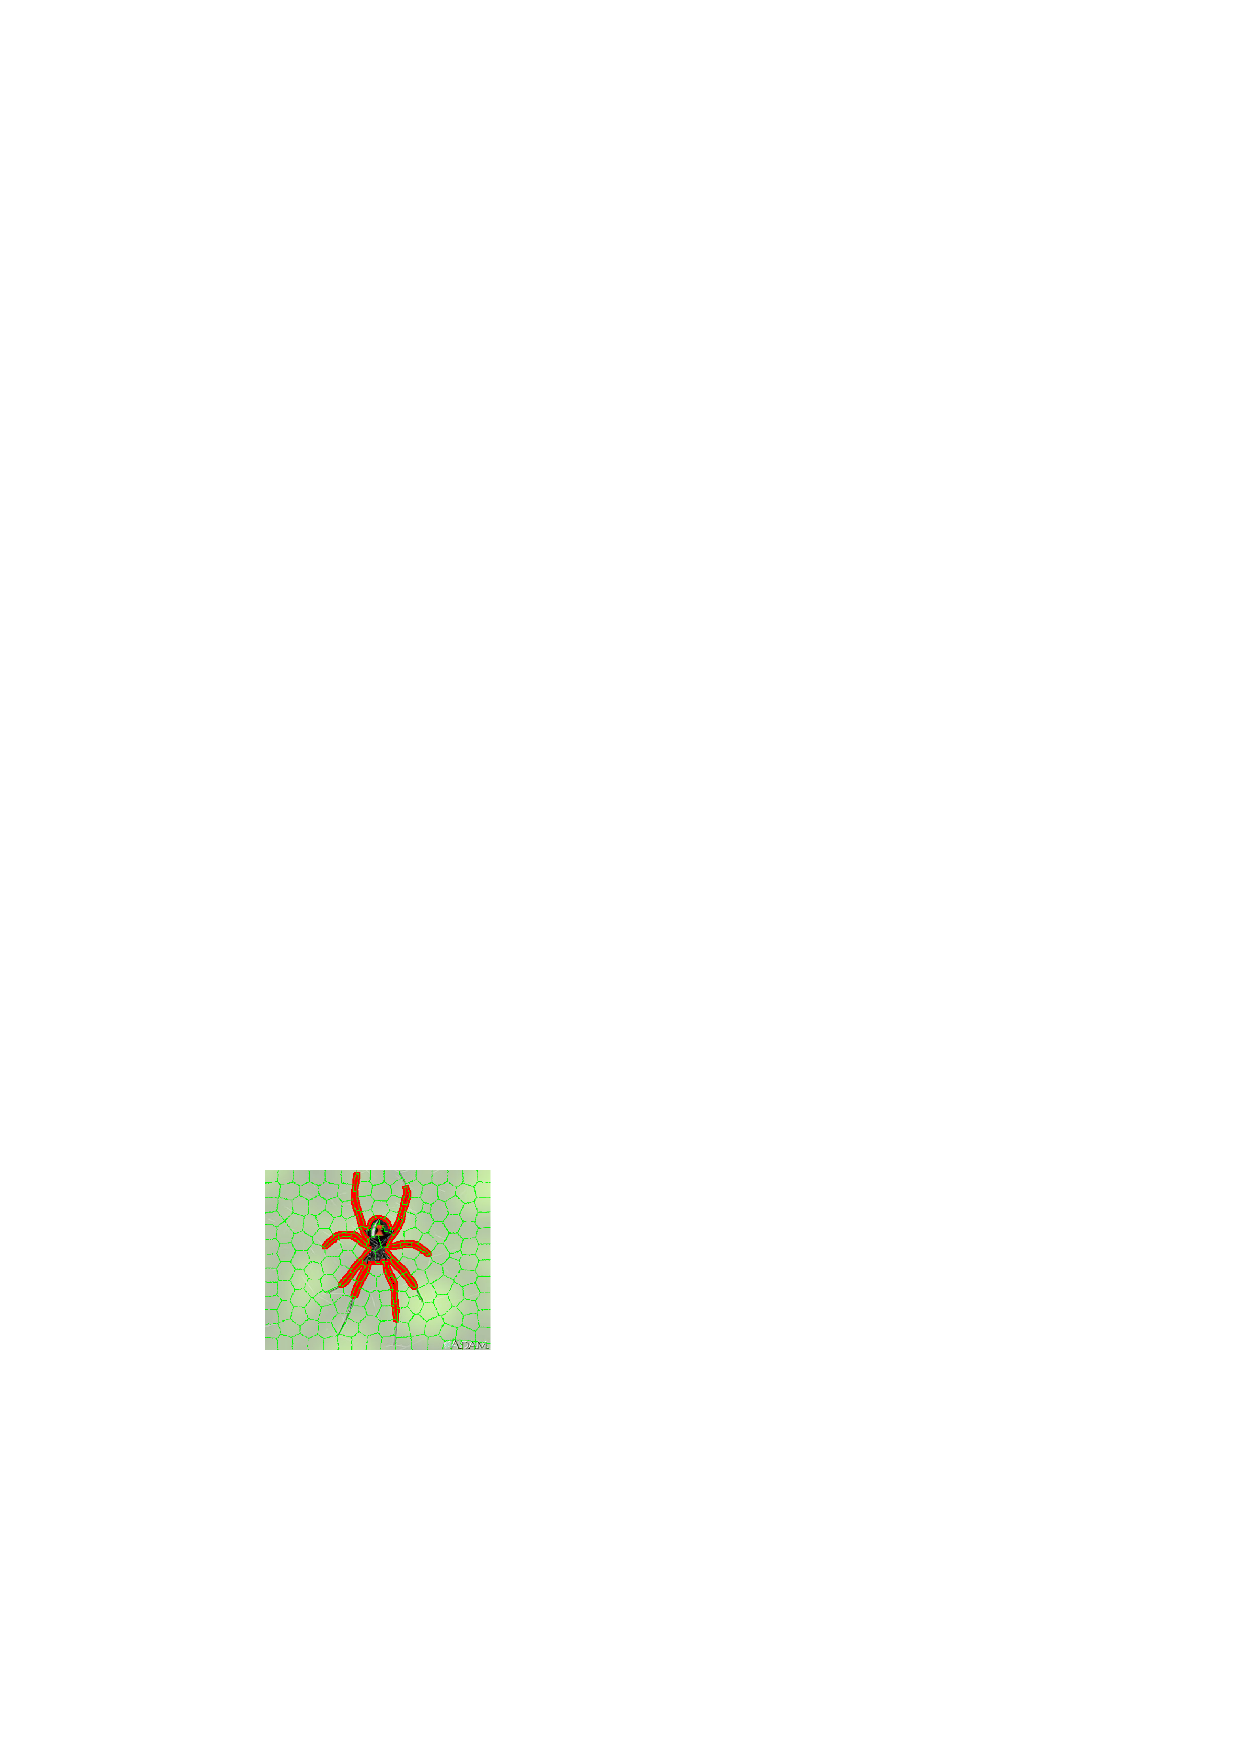
\includegraphics[width=0.22\textwidth]{figs/sp_prob2.pdf}
{\footnotesize\textit{g}}\includegraphics[width=0.22\textwidth]{figs/lizard_tail.pdf}
{\footnotesize\textit{h}}\includegraphics[width=0.22\textwidth]{figs/giraffe_cons.pdf}

\caption{(a) An image of a landscape and in (b) we observe open curves that define the various mountain ranges and tree-line. c) An image of a sculpture and in (d) the various internal open-ended contours that define the structure of the piece. (e) Ground-truth annotations of the car~\cite{Guo:Kimia:POCV12} show that humans perceive all types of contours. f) We show an example from the output of ~\cite{Levinshtein:etal:IJCV12} where all that can be recovered is closed curves. g) The tail (shown in dark pink) of the lizard interacting with the internal contours enclosing each spot create the formation of T-junctions. h) The two contours capturing the silhouette of the giraffe meet at a T-junction. }

%% f) We observe how curves of various configurations are recovered in a contour-based representation of the car.}

 \label{fig:sp_probs2}
%\vspace{-0.751cm}
\end{figure}

The second fundamental difficulty with superpixel contours is due to its construction as the boundary is of closed regions. As such, several types of contours are automatically excluded: \emph{(i)} open contours, as shown in Figure~\ref{fig:sp_probs2}\textcolor{red}{(a-e)} cannot be represented. This is in contrast to the innate capability of such contours to capture closed cues, as exemplified by the approach in~\cite{Levinshtein:etal:IJCV12} where the initial set of disconnected superpixel contour fragments, shown as green in Figure~\ref{fig:sp_probs2}\textcolor{red}{(f)}, merge into a single closed contour by maximizing the appearance difference between background and foreground over the space of all closed curves, Figure~\ref{fig:sp_probs2}\textcolor{red}{(f)}. \emph{(ii)} T-junction where the superpixel contours break the continuous top of ``T'' into two contours with no clear indication as how to recover the grouping of split contours, Figure~\ref{fig:sp_probs2}\textcolor{red}{(g-h)}.  Reasoning with all types of contours namely, closed, open, and junction-forming, requires an augmented representation.  





%% their inability to represent whether individually or grouped the vide variety of contour types. If we look at the human ground-truth markings on the car and tiger, Figure~\ref{fig:sp_probs2}\textcolor{red}{b-d}, we notice that besides the silhouette internal open-ended contours have been delineated along with junction-forming (T,X,Y) contours defined by the interaction of the silhouette with internal markings. If we revisit Figure~\ref{fig:sp_probs1}\textcolor{red}{a-b} we see that each individual superpixel contour is connected to other contours which limits open ended contours and furthermore while junctions bound each superpixel contour it is not clear how to recover contours that form T, Y, or X junctions.  To illustrate this problem we look at a recent paper~\cite{Levinshtein:etal:IJCV12} that advocates for reasoning with superpixel contours. Briefly, this paper groups an 


%% Another fundamental difficulty of superpixels is the inability to represent non-closed regions. To recover non-closed regions and their corresponding boundary requires that the superpixel boundaries need to have a start point and an endpoint \ie an open contour. To illustrate this problem we look at a recent paper~\cite{Levinshtein:etal:IJCV12} that advocates for reasoning with superpixel contours. Briefly, this paper groups a set of disconnected superpixel contour fragments into a single closed contour that maximizes the appearance difference between background and foreground, Figure~\ref{fig:sp_issues}. Observing Figure~\ref{fig:sp_issues} we can see that recovering closed contours amounts to merging 


%%  to organize them into larger closed contours, This brings us to our second drawback of utilizing superpixels is the inability to represent non-closed regions. To recover non-closed regions, such as one leg of the spider of the head of the horse, is even more complicated as it amounts to considering not cycles but all possible paths, blue curve in Figure~\ref{fig:sp_issues}\textcolor{red}{a}, within this graph. This is not only computationally intractable, but also the representation is not amenable to such outputs. 


%% Other strategies include using a coarser number of superpixels or adaptive sized superpixels [Add ref to Chellapa] that lead to less fragmentation. Regardless of approach there will always be some intermingling of veridical and non-sensical boundaries, as region grouping processes are forced to accumulate region information all across the image. The classic example of this is the sky problem where by a large homogeneous portion of the image is artificially broken into many pieces. Even if we adopt an adaptive approach it is unlikely that a superpixel would be of the appropriate size and shape to cover such a large territory. Furthermore, even if we assume these strategies lead to a perfect determination of which boundaries are veridical and which are not, we still would not know which pieces of object boundaries go together. Given that it is unlikely that a single superpixel will cover an object of interest the various delimiters have to be merged similar to an edge linking process or equivalently the consistent regions have to be grouped. In either approach, the output of this process is biased to producing a closed contour. 


 
%% \begin{figure}[ht]
%% \begin{center}
%% {\footnotesize\textit{a}}\includegraphics[width=0.22\textwidth]{figs/sp_prob1.pdf}
%% {\footnotesize\textit{b}}\includegraphics[width=0.22\textwidth]{figs/sp_prob2.pdf}
%% \end{center}
%% \caption{All images courtesy of~\cite{Levinshtein:etal:IJCV12}. a) A small set of superpixels with the red cycle indicating a possible closed contour to consider. The blue path represents the boundary of a non-closed region. b) Examples of a closed boundary recovered using the method of~\cite{Levinshtein:etal:IJCV12}. }
%% \label{fig:sp_issues}
%% \end{figure}

%% Determining the object boundary utilizing superpixels is a difficult task, irregardless of whether the goal is a closed region or not. The task of recovering the contour amounts to merging the various delimiters, which given a superpixel graph amounts to considering all possible cycles~\cite{Levinshtein:etal:IJCV12}, Figure~\ref{fig:sp_issues}. The red-dashed line in Figure~\ref{fig:sp_issues}\textcolor{red}{a} is one possible cycle out of the many combinations that could possibly exist. We can see successful recovery of the closed contour in Figure~\ref{fig:sp_issues}\textcolor{red}{b}, but the subsequent figure depicts an erroneous recovered boundary despite the superpixels perfectly following the silhouette of the horse. 

%% Representing non-closed regions can be not effectively done by a region based description alone. Superpixels and there consistent boundaries can only represent closed curves, 


%% Figures~\ref{fig:sp_probs1}\textcolor{red}{b,c} depict the superpixel boundaries colored in white. If all superpixel boundaries were veridical we would expect the ground-truth pixel map to agree with 



%% Superpixels are perceptually consistent units that adhere well to image boundaries. 

%% serve as the basic unit of reasoning for many region based \emph{object proposal} schemes.


%% They are a compact representation that adhere well to natural image boundaries. Given that each superpixel 


%% As discussed earlier, we would like to reason with types of object signatures: namely regios and contours. One the surface it would seem that superpixels 

%% Superpixels are a popular intermediate from as they capture both regional and contour aspects. 


%% fundamental drawback in using superpixels as an intermediate representation is that 


%% the outer perimeter of each region 

%% They are a compact representation that capture both regional and contour aspects. 

%% Object proposals algorithm generate a wide variety of candidate regions by merging superpixels based on some measure of regional 

%% As discussed earlier grouping methods generate object proposals by merging superpixels based on some notion of regional homenginity. 

%% Superpixels are the basic unit of reasoning about object proposals resulting from grouping pixels into region fragments based on appearance homogeneity. The other signature, though traditionally ignored, of superpixel is the closed boundary that serves as the perimeter of grouped pixels. 

%% enjoy many desirable properties which make them useful for applications even beyond generating object proposals. They are \emph{computational efficient}: the complexity of dealing with hundreds or thousands of pixels in an image is reduced to only a few hundred superpixels. Superpixel maps are \emph{representationally efficient} as pairwise constraints between units, while only for adjacent pixels on the pixel grid, can now model much longer-range interactions between superpixels.  And finally the representation is \emph{near-complete} as there is very little loss in moving from the pixel grid to the superpixel map. 



%% If we look at Figure~\ref{fig:sp_probs1} we see an image 



%% The problem of determining veridical and non-sensical boundaries within a superpixel map is a well known problem. Traditionally this has been dealt with by looking for the presence or absence of contour evidence, predominantly in the form of \emph{Pb} or \emph{gPb} probabilities, for each delimiter. The basis for merging two superpixels, among any other cues, then becomes a function of the contour strength of their separator \emph{i.e} the stronger the evidence the less likely they should be merged as it is indicative of an object boundary. However, while the merging process implicitly considers the type of boundary, this information is not made explicit in the final representation. This subtle distinction makes superpixels inappropriate for our purpose. To illustrate this point, in Figures~\ref{fig:mvf_justify}\textcolor{red}{(a-b)} we see a piece of a horse which is the output of some superpixel merging process and its associated closed boundary. This dual representation of region and boundary is only half correct. While the regional information is highly plausible, the closed contour indicates that this is a whole object rather than a part of something else. What we need is illustrated in Figure~\ref{fig:mvf_justify}\textcolor{red}{c}, where by the closed boundary is split up into a red veridical contour and a blue artificial contour. The superpixel representation is not amenable to such outputs. To recover non-closed regions or parts and their corresponding boundary requires that the delimiters between superpixels need to have a spatial ordering, a start point and endpoint. To call superpixel boundaries as contours is a gross misnomer as they amount to set of unorganized pixels which is sufficient for recovering closed boundaries, but not for non-closed boundaries. Given these drawbacks, the regional representation we desire is one where the true and artificial boundaries are clearly delineated, where each individual boundary is an ordered set of pixels or edges, and finally where each individual boundary's shape and length are maximized to support image evidence. The latter two are precisely what an unorganized set of contours gives us. 
   

%% \begin{figure}[ht]
%% \centering
%% {\footnotesize\textit{a}} \includegraphics[width=0.30\linewidth]{figs/horse_frag_bw.png} 
%% {\footnotesize\textit{b}} \includegraphics[width=0.30\linewidth]{figs/orig_closed.pdf} 
%% {\footnotesize\textit{c}} \includegraphics[width=0.30\linewidth]{figs/orig_actual.pdf}
%% \caption{a) The regional description of a piece of a horse. b) Its associated closed boundary. c) Representing the part by its artificial and real boundaries. }
%% \label{fig:mvf_justify}
%% \end{figure}



%% Other strategies include using a coarser number of superpixels or adaptive sized superpixels [Add ref to Chellapa] that lead to less fragmentation. Regardless of approach there will always be some intermingling of veridical and non-sensical boundaries, as region grouping processes are forced to accumulate region information all across the image. The classic example of this is the sky problem where by a large homogeneous portion of the image is artificially broken into many pieces. Even if we adopt an adaptive approach it is unlikely that a superpixel would be of the appropriate size and shape to cover such a large territory. Furthermore, even if we assume these strategies lead to a perfect determination of which boundaries are veridical and which are not, we still would not know which pieces of object boundaries go together. Given that it is unlikely that a single superpixel will cover an object of interest the various delimiters have to be merged similar to an edge linking process or equivalently the consistent regions have to be grouped. In either approach, the output of this process is biased to producing a closed contour. This brings us to our second drawback of utilizing superpixels is the inability to represent non-closed regions. To recover non-closed regions, such as one leg of the spider of the head of the horse, is even more complicated as it amounts to considering not cycles but all possible paths, blue curve in Figure~\ref{fig:sp_issues}\textcolor{red}{a}, within this graph. This is not only computationally intractable, but also the representation is not amenable to such outputs. 

 
%% \begin{figure}[ht]
%% \center
%% {\footnotesize\textit{a}}\includegraphics[width=0.15\textwidth]{figs/sp_prob1.pdf}
%% {\footnotesize\textit{b}}\includegraphics[width=0.15\textwidth]{figs/sp_prob2.pdf}
%% {\footnotesize\textit{c}}\includegraphics[width=0.15\textwidth]{figs/sp_prob3.pdf}
%% \caption{All images courtesy of~\cite{Levinshtein:etal:IJCV12}. a) A small set of superpixels with the red cycle indicating a possible closed contour to consider. The blue path represents the boundary of a non-closed region. b)c) Examples of successful and erroneous recovery of the object silhouette. }
%% \label{fig:sp_issues}
%% \end{figure}

%% Determining the object boundary utilizing superpixels is a difficult task, irregardless of whether the goal is a closed region or not. The task of recovering the contour amounts to merging the various delimiters, which given a superpixel graph amounts to considering all possible cycles~\cite{Levinshtein:etal:IJCV12}, Figure~\ref{fig:sp_issues}. The red-dashed line in Figure~\ref{fig:sp_issues}\textcolor{red}{a} is one possible cycle out of the many combinations that could possibly exist. We can see successful recovery of the closed contour in Figure~\ref{fig:sp_issues}\textcolor{red}{b}, but the subsequent figure depicts an erroneous recovered boundary despite the superpixels perfectly following the silhouette of the horse. 
%% Representing non-closed regions can be not effectively done by a region based description alone. Superpixels and there consistent boundaries can only represent closed curves, 



 
%% Superpixels are the basic unit of reasoning about object proposals resulting from grouping pixels into region fragments based on regional homogeneity~\cite{Ren:Malik:ICCV03,Ahuja:Todorovic:CVPR08,malisiewicz:bmvc07}.  

%% One main difficulty with the boundaries of  superpixels is that it is not clear which portions are meaningful boundaries and which are simply delimiters of the grouped pixels. These latter contours are more a product of the dynamics of the grouping process than an indicator of underlying structure, \eg, the pink-yellow boundary in Figure~\ref{figure:combinatorial:possibilities}b. The ambiguity created by the presence of these artifactual boundaries among meaningful boundaries limits the use of grouping based on contours.
% \begin{figure}[!h]
% \centerline{
% {\footnotesize\textit{a}}
% \includegraphics[height=0.22\linewidth]{figs/shaded-torus.png}
% {\footnotesize\textit{b}}
% \includegraphics[height=0.22\linewidth]{figs/shaded-torus-segmentation.png}
% {\footnotesize\textit{c}}
% \includegraphics[height=0.22\linewidth]{figs/koenderink-contour-end-1.png}
% {\footnotesize\textit{d}}
% \includegraphics[height=0.22\linewidth]{figs/picasso-hands.png}
% %\includegraphics[height=0.2\linewidth]{figs/Prometheus-Brennan.png}
% %\hspace{-0.1cm}\includegraphics[height=0.2\linewidth]{figs/Prometheus-Brennan-k_12.pdf}
% }
%   \caption{\FigureFont
%   \label{fig:region:issues}
%   (a,b) Region-based grouping produce ``superpixels'' with boundaries composed
%   of both meaningful contours as well as artifactual boundaries resulting
%   from the dynamics of the grouping process which delimits adjacent regions
%   but does not lay claim to boundary-hood. Superpixels cannot represent
% contours that end, (c) from \cite{Koenderink:VanDoorn:Perception82} and
% (d) a Picasso drawing.   }
% %\vspace{-0.35cm}
%\end{figure}

%% Another fundamental difficulty in region-based representation is the inability to represent contours that end, Figure~\ref{figure:combinatorial:possibilities}d, which among others,  significantly limits the detection of gaps, \eg, as present in the bottom and top portions of the inner and outer circles in the shaded torus of Figure~\ref{figure:combinatorial:possibilities}a; It is difficult to work with gaps in the superpixel representation, Figure~\ref{figure:combinatorial:possibilities}b, because end-points of contours are not represented. Despite their limitations, superpixels do have their strengths, namely they exhibit neighborhood structure. For any partitioning ( in the formal sense) of the image, a region adjacency graph defines neighborhood relations between partitions or superpixels. 
  
% \begin{figure}[!h]
% {\footnotesize\textit{a}}
% \includegraphics[height=0.076\linewidth]{figs/good-continuation-1.png}
% {\footnotesize\textit{b}}
% \includegraphics[height=0.076\linewidth]{figs/good-continuation-2.png}
% {\footnotesize\textit{c}}
% \includegraphics[height=0.076\linewidth]{figs/good-continuation-3.png}
% {\footnotesize\textit{d}}
% \includegraphics[height=0.076\linewidth]{figs/good-continuation-4.png}
% {\footnotesize\textit{e}}
% \includegraphics[height=0.076\linewidth]{figs/good-continuation-5.png}
% {\footnotesize\textit{f}}
% \includegraphics[height=0.076\linewidth]{figs/appearance-continuity-1.png}
% {\footnotesize\textit{g}}
% \includegraphics[height=0.076\linewidth]{figs/appearance-continuity-2.png}
%   \caption{\FigureFont
%   \label{fig:contour:continuity}
%   The Gestalt notion of good continuation disambiguates between  the two situations in (a,b), but cannot detect interaction from related contours
% (c-e), which require a notion of figural continuity. (f,g) Appearance continuity is another significant cue. 
%   }
% \end{figure}


%% \begin{figure}[!h]
%% %\vspace{-0.5cm}
%% \centering
%%  % {\footnotesize\textit{(a)}} \includegraphics[width=0.1225\linewidth]{figs/place_holder.pdf}
%% {\footnotesize\textit{a}}
%% \includegraphics[width=0.28\linewidth]{figs/shaded-torus.jpg}
%% {\footnotesize\textit{b}} \includegraphics[width=0.28\linewidth]{figs/shaded-torus-segmentation.jpg}
%% {\footnotesize\textit{c}} \includegraphics[width=0.28\linewidth]{figs/torus_contours_multi_color.pdf}
%% \\
%% %{\footnotesize\textit{(d)}}\includegraphics[width=0.1225\linewidth]{figs/contour-but-not-region.png}
%% %{\footnotesize\textit{(e)}} \includegraphics[width=0.1225\linewidth]{figs/competition-between-two-regions.png}
%% {\footnotesize\textit{d}} \includegraphics[height=0.15\textwidth]{figs/picasso-hands.jpg}
%% \vbox{
%% \hbox{
%% {\footnotesize\textit{e}}
%% \includegraphics[height=0.15\linewidth]{figs/contour-but-not-region.jpg}
%% %\includegraphics[height=0.08\linewidth]{figs/figural-continuity-1.png}
%% {\footnotesize\textit{f}}\includegraphics[height=0.15\linewidth]{figs/figural-continuity-2.jpg}
%% %{\footnotesize\textit{f}}\includegraphics[height=0.06\linewidth]{figs/good-continuation-1.png}
%% }
%% \hbox{
%% {\footnotesize\textit{g)}}\includegraphics[height=0.1\linewidth]{figs/good-continuation-3.jpg}
%% %{\footnotesize\textit{h\includegraphics[height=0.056\linewidth]{figs/good-continuation-2.png}}}
%% {\footnotesize\textit{h}}\includegraphics[height=0.1\linewidth]{figs/good-continuation-4.jpg}
%% }
%% }
%% % \hbox[2cm]{\includegraphics{figs/one-contour-between-two-others.png}
%% % \includegraphics{figs/one-contour-supports-another.png}
%% % \includegraphics{figs/one-gap-supports-another.png}}
%% {\footnotesize\textit{i}}\includegraphics[width=0.23\linewidth]{figs/torus_contours_shocks.pdf}
%% %\textit{k} \hspace{-0.0512cm}
%% %  \includegraphics[width=0.135\linewidth]{figs/place_holder.pdf}
%% %\vspace{-0.2cm}
%%   \caption{ (a,b) The use of superpixels is not appropriate in our
%% approach because (i) artifactual boundaries (say the contour between pink
%% and yellow regions) are not differentiated from actual boundaries,   and
%% (ii) the representation does not identify gap endpoints,  required to identify completion candidates. (c) contour fragment endpoints identify potential gaps. (d) many image contours are not closed (e-f)
%% appearance continuity is a powerful cue in grouping. The spatial interaction
%% among contours prevents some gaps from being considered (g), while supporting
%% others\ (h). (i) The shock graph pairs image contours. }
%%  \label{figure:combinatorial:possibilities}
%% %\vspace{-0.751cm}
%%  \end{figure}

\subsection{Unorganized Set of Curve Fragments}

Reasoning with curve fragments is the second of the classic complementary organization of visual processes into region-based and contour-based. However, the use of curve fragments as a basis for reasoning about images has been largely confined to the perceptual grouping community. Gestalt laws such as good continuation have been formulated in terms of curves. Perhaps this is because reasoning with appearance-similarity requires a notion of regions which is lacking in a contour-based representation, except in the special case of a closed contour. There is some work on using contour fragments for object recognition~\cite{Shotton:Blake:Cipolla:iccv05,Ferrari:Fevrier:Jurie:Schmid:PAMI08, Kumar:Torr:Zisserman:BMVC04}. These papers were unable to generalize to objects whose primary cue is appearance and furthermore were restricted to databases, ETHZ Shape Dataset~\cite{Ferrari:etal:IJCV10} where the objects were depicted exclusively from a side viewpoint, \ie side of a horse, side of a giraffe, where the silhouette contours are most discriminative. However, no object proposal methods use curve fragments as a basis for forming objects or object parts, as we propose here. A key shortcoming preventing this is the observation that, in contrast to superpixels which enjoy a spatial organization via the region-adjacency graph, contour fragments lack a neighborhood structure. The lack of spatial organization renders the practical formulation of Gestalt laws challenging as it is not a-priori clear which pair of curve fragments need to interact. We use the shock graph, which is traditionally a representation of closed curves, to represent the spatial organization of contour fragments, as described next. 

%% Curve fragments provide an alternative set of grouping options when compared to superpixels. One of the major strengths of utilizing curve fragments as compared to regional processes is the reduced set of false positives. In both superpixels and curve fragments we have a similar problem, where by we end up with some real boundaries interspersed with spurious boundaries. While in the case, of superpixels a large portion of the boundaries are due to the artificial dynamics of the region process, in the case of contours this is minimized due to the process being inherently based on image evidence, bottom row of Figure~\ref{fig:sp_probs1}. Along with the reduced set of false positive the contour formation process is generic and leads to a wide variety of curve configurations, Figure~\ref{fig:sp_probs2}\textcolor{red}{f}. 
 %% The classic example of this is the sky problem where by a large homogeneous portion of the image is artificially broken into many pieces as region grouping processes are forced to accumulate region information all across the image. In the case of contours, this situation is minimized as contours are adaptive in the sense as they only fire where image evidence presents itself. 

%% And finally unlike superpixels boundaries, curve fragments represent an ordered set of edgels. \textcolor{red}{To Ben: Why is that contours have less artificial or spurious boundaries compared to superpixels? }

%% Curve fragments provide an alternative set of grouping options when compared to superpixels. One of the major strengths of utilizing curve fragments as compared to regional processes is the reduced set of false positives. In both superpixels and curve fragments we have a similar problem, where by we end up with some real boundaries interspersed with spurious boundaries. While in the case, of superpixels a large portion of the boundaries are due to the artificial dynamics of the region process, in the case of contours this is minimized due to the process being inherently based on image evidence. The classic example of this is the sky problem where by a large homogeneous portion of the image is artificially broken into many pieces as region grouping processes are forced to accumulate region information all across the image. In the case of contours, this situation is minimized as contours are adaptive in the sense as they only fire where image evidence presents itself. And finally unlike superpixels boundaries, curve fragments represent an ordered set of edgels. \textcolor{red}{To Ben: Why is that contours have less artificial or spurious boundaries compared to superpixels? }

%% The use of curve fragments as a basis for further reasoning has been predominantly confined to the perceptual grouping community. As a consequence of this, the majority of gestalt laws such as proximity, good continuation, and symmetry have been formulated in terms of curves as compared to other intermediate-level representations. This represents a strong reason for using contours as these laws which lead to ``good form'' can be effectively be implemented in a computational framework. 

%% Despite the appealing characteristics of curve fragments, they do have their drawbacks. The major and most obvious drawback of contours is that they can not represent regions. Ignoring the special case of a closed contour, a general set of image contours renders reasoning with regional information and generating regional proposals impossible. The other major drawback of working with contours is that a set of contours lacks any organization, \emph{i.e.}, neighborhood structure. Unlike superpixels which have an inherent organization captured by a region-adjacency graph, it is not clear how to define neighbors or the idea of proximity with a set of contours. Even more the elegant formulation of gestalt laws in terms of curves is very difficult to implement in practice due to this lack of spatial organization. This requires a representation where contours and their neighborhood structure are explicitly captured. 

%% In summary, superpixels represent both a region and a boundary. However, as we have shown the vast majority of these superpixel boundaries are artificial. If we exclusively use contours the vast majority are veridical, but it limits our ability to recover and reason with regions. What is needed is a integrated representation that represents the veridical contours, coupled with the regions those contours bound. 



 %% Contours like superpixel's are complete representations when it comes to closed regions but are incomplete representations when it comes to explaining non-closed portions of the image. Revisiting Figure~\ref{fig:mvf_justify}\textcolor{red}{c} we see that the final representation we want is composed of a region bounded by two contours. While a contour representation can represent the red contour, it is unable to represent the blue curve which is a region delimiter and not the output of edge linking. 



%% Many ideas from the gestalt school of thought have been formulated in terms 


%% Curve fragments are often viewed as a precursor to figure-ground segregation and for formulating the Gestalt notion of good continuation,Figure~\ref{fig:mvf_justify}\textcolor{red}{c}, \eg, using elastica \cite{Mumford:Elastic:1994,Williams:Jacobs:NC95} or using the Euler Spiral \cite{Kimia:Euler:Spiral:IJCV03}.






%%  Good continuation is used to disambiguate grouping choices. However, a contour representation cannot take into account the interaction of nearby contours  which may invalidate a completion, Figure~\ref{figure:combinatorial:possibilities}g, or which continuations group the wrong sides of a figure, Figure~\ref{figure:combinatorial:possibilities}e. This representation also cannot strongly encourage the groupings in Figure~\ref{figure:combinatorial:possibilities}h, as it should because it cannot represent ``\textit{figural continuity}'', a very  powerful cue in disambiguating conflicting groupings. Figural continuity requires good continuation of \textit{a pair of contours} that are bound together and that continue together. Finally, another proposed powerful Gestalt cue is   \textit{appearance continuity}, which states that two fragments' grouping depends on the continuity of their appearance, Figure~\ref{figure:combinatorial:possibilities}f. 


\subsection{Shock Graph}
\label{sec:shock_graph}

We propose that the shock graph of contour fragments addresses major shortcomings of each of the two distinct but complementary representations: Superpixels do not explicitly distinguish image curves from region grouping delimiters, and an unorganized set of contours have no notion of regions or neighborhood relationship. First observe that the shock graph can associate a region to each shock graph segment. Given many contour fragments, how can we assign a pixel to a particular contour? The grassfire analogy claims a region for each contour by distance to contours, \ie, a pixel is assigned to the closest contour. In other words, a contour extends its influence as far as the medial axis, see Figure~\ref{fig:ma_motivate}. The Medial Axis therefore “binds” together a pair of contours and identifies the region between them.  In this view the medial axis segment is really just a joint representation of a pair of contours and their intervening region. The shock graph~\cite{Kimia:etal:ECCV:Book,Kimia:etal:Shape:Series:I,Giblin:Kimia:Reconstruction:PAMI03}, a refinement of the Medial Axis, which arises from viewing the medial axis as the locus of singularities (shocks) formed in the course of wave propagation (grass-fire) from a pair of contour elements, Figure~\ref{fig:ma_vs_sg}, and its corresponding computation capture this pairwise relationship between contour elements. Formally, 

\begin{figure}[ht]
\center
a)\raisebox{2.5\height}{\includegraphics[width=0.2\textwidth]{figs/ma_step_1.pdf}}
b)\raisebox{1.8\height}{\includegraphics[width=0.2\textwidth]{figs/ma_step_2.pdf}}
c)\fcolorbox{white}{white}{\includegraphics[width=0.2\textwidth]{figs/ma_step_3.pdf}}
d)\fcolorbox{white}{white}{\includegraphics[width=0.2\textwidth]{figs/ma_step_4.pdf}}
\caption{Motivating the use of the medial axis to capture the regional information of \emph{C1}, depicted in Figures (a) and (b) with another interacting contour \emph{C2} illustrated in (c). (d) The medial axis in the absence of any other information, is the bisector of two regions. } 
\label{fig:ma_motivate}
\end{figure}

\begin{figure}[ht]
\center
\includegraphics[width=0.6\textwidth]{figs/shocks-ma-new.pdf}
\caption{From~\cite{Giblin:Kimia:IJCV03}. The advantage of the shock graph over medial axis is its qualitative description of the boundary: given a medial axis segment any of the six shapes in the top row can occur, while a shock graph segment (a monotonically flowing subsegment of the medial axis) qualitatively represents one type of shape.}
\label{fig:ma_vs_sg}
\end{figure}

\begin{definition}
\label{def:sg}
The shock graph is a directed attributed relational graph, $G=(V,E,A)$, where $V$ is the vertex set of shock nodes, $E$ is the edge set of shock segments, and $A$ is the continuous intrinsic geometry and classification labels, specifically $A$ is the set of unary attributes $a_i$ attached to each vertex $v_i \in V$, namely normal, tangent, time of formation and discrete labels sink, source, or junction. The shock link binary attributes $a_{ij}$ attached to each $e_k=(v_i,v_j) \in E$ consist of length, curvature, and acceleration and discrete labels degenerate, semi-degenerate, or regular. 
\end{definition}





%% We answer this in two parts. First we solve the problem, of how to represent contours while recovering their neighborhood relationship? This relationship is precisely captured by the shock graph! 




There are many approaches to computing the medial axis/shock-graph ranging from topological thinning methods, distance transform methods, curve evolution schemes, and finally computational geometric algorithms.  We adopt the approach of~\cite{Tamrakar:Kimia:Shock}, which is  a hybrid between curve evolution and computational geometric techniques. The main advantage of this scheme over curve-evolution based schemes~\cite{Tek:Wave:Propagation:IJCV03} is that it is designed to work not only with a set of \emph{closed curves} but also with a set of \emph{open (non-closed) curves}. In what follows we highlight the main aspects of computing the shock graph to the extent that it is relevant to this thesis. 



%% \begin{figure*}[ht]
%% \center
%% a)\includegraphics[width=0.3\textwidth]{figs/sc_step1.pdf}
%% b)\includegraphics[width=0.3\textwidth]{figs/sc_step2.pdf}
%% c)\includegraphics[width=0.3\textwidth]{figs/sc_step3.pdf}
%% \caption{A pair of \textcolor{red}{contours} and their bisector. Sub figures b and c show how the introduction of  a new source, invalidates the bisector and determines the valid portion. Also notice the formation of shock nodes at the intersection of bisector curves. } 
%% \label{fig:sc1_steps}
%% \end{figure*}


Formally, the computation of shocks from an unorganized set of curve fragments relies on two key ideas. First, since the shocks arising from points and lines can be analytically computed, the curve fragments can be first approximated by a polyline, namely, a set of line segments that share end points; there are well-known algorithms to achieve this by specifying the expected error~\cite{vxl:webcite}. It is well-known that the bisector of two points is a line, the bisector of two lines is a line, and the bisector of a point and a line is a parabola, Figure~\ref{fig:bisect}. The dynamics of shocks moving on this bisector are less trivial but they can also be calculated analytically. The geometry and dynamics of shocks arising from any isolated pair from a collection of point and line sources is therefore readily available in analytic form and this saves in computation time and provides numerical stability robustness. 

\begin{figure}[ht]
\center
a)\includegraphics[width=0.221\textwidth]{figs/point-point-fixed.pdf}
b)\includegraphics[width=0.4\textwidth]{figs/line-line-fixed.pdf}
c)\includegraphics[width=0.221\textwidth]{figs/point-line-fixed.pdf}

\caption{Analytic computation of shocks from polylines requires shocks from (a) point-point (b) line-line and (c) point-line pairs. Boundary “sources” are shown in red, shocks are shown in green, and the rays connecting boundary sources to respective shocks are shown in dashed lines. These computations assume only a pair of sources with no interaction from other sources so all shocks go off to infinity.  } 
\label{fig:bisect}
\end{figure}

The second key idea is the use of a wave propagation and shock propagation to piece together shocks from multiple pairs of sources in a highly efficient way. Observe that the union of all shock-graph of isolated pairs of sources is a superset of the shock graph of the union of boundary sources, \eg, as in the bisectors shown in grey and green which is a superset of the shock graph shown in green in Figure~\ref{fig:sc2_steps}{(h)}. Consider first the shock points on a bisector of a pair of boundary sources: a shock point is valid if no other waves from sources other than its own sources reach there. In other words, a shock is valid if its time of formation (distance to its sources) is earlier than the time of propagation (distance) to any earlier other source. Since the shock path on any bisector has an initial shock point (shock source), the extent of the valid shock path can be determined by first examining the validity of the shock source itself, the first shock point to form in time. Since a valid shock path can only be potentially terminated at the intersection of two shock paths, these are the only points that need to be examined. This is a key distinction since it discretizes the continuous propagation into a discrete propagation. Thus, the algorithm first computes all shock sources, an $N^2$ computation for $N$ boundary sources, and considers shock paths for the sources in order of time. 

\begin{figure*}[ht]
\center
{\footnotesize\textit{a}}\includegraphics[width=0.235\textwidth]{figs/incremental-voro-02-01.pdf}
{\footnotesize\textit{b}}\includegraphics[width=0.235\textwidth]{figs/incremental-voro-02-02.pdf}
{\footnotesize\textit{c}}\includegraphics[width=0.235\textwidth]{figs/incremental-voro-03-01.pdf}
{\footnotesize\textit{d}}\includegraphics[width=0.235\textwidth]{figs/incremental-voro-03-02.pdf}
{\footnotesize\textit{e}}\includegraphics[width=0.235\textwidth]{figs/incremental-voro-04-01.pdf}
{\footnotesize\textit{f}}\includegraphics[width=0.235\textwidth]{figs/incremental-voro-04-02.pdf}
{\footnotesize\textit{g}}\includegraphics[width=0.235\textwidth]{figs/incremental-voro-05-01.pdf}
{\footnotesize\textit{h}}\includegraphics[width=0.235\textwidth]{figs/incremental-voro-05-02.pdf}

\caption{This figure illustrates the incremental steps of shock computation for a set of \textcolor{red}{red input curves}. At each step infinite length \textcolor{cyan}{cyan bisector curves} between a new boundary element and each of the previous boundary elements are computed. The finite true bisectors after the limiting process are shown in \textcolor{green}{green} with the removed shock branches shown in \textcolor{gray}{gray}. The \textcolor{green}{green shock links} represent the valid portion of bisector curves.} 
\label{fig:sc2_steps}
\end{figure*}


Figure~\ref{fig:sc2_steps} illustrates this process. Consider two fragments, $C_1$ and $C_2$ whose potential shock path is shown in cyan in (a).  For the purpose of illustrating the second key idea, namely using propagation to compute the shock graph, the contour fragments are not restricted to be polylines and can take any form. Also, these are sketches and not accurate in scale. Since there are no other interacting shock paths, the entire shock path is validated and shown in green. Next, suppose that a third contour fragment $C_3$ is added to the pool of curve fragments. The interaction of the new-comer $C_3$ with $C_1$ and $C_2$ generates two potential shock paths shown in cyan in (c). The intersection of these shock paths with existing shock paths create shock junctions, which are the only potential terminators of a shock path. In this particular case there is only one shock junction, with each of the three shock paths flowing into the shock junction. Since the continuation of each shock path has a time exceeding the time of the waves reaching there from another source, all three shock paths are terminated, as shown in (d). In other cases it can happen that two shock branches flow into a junction and one shock branch flows out. In this case the two branches flowing into the junction are terminated in which the shock branch flowing out only begins at the junction as its source. It can also happen that the entire shock path is invalid, say if the two sources on the opposite sides of an image with many sources in between. Consider now $N$ boundary sources. The process of shock computation can be implemented by first computing the shock path for a pair of boundary sources, and then considering a third, a fourth, \etc. , Figure~\ref{fig:sc2_steps}. While this can be done in any order, the most efficient order is one that considers the earliest forming shocks first. 



The practical implementation of these two ideas is realized through the construction and visitation of two time-ordered lists. The first list contains the \emph{candidate} sources that are initially pre-computed and has size $N^2$ and is a superset of all possible source nodes in the shock-graph. The second list is the \emph{active} shock list, the list of shocks under propagation, and is initially empty. The algorithm proceeds by visiting the first element in the \emph{candidate} source list and initializing a pair of child shocks (outgoing flow) where each child has a start time equivalent to the time of formation of the source node and an end time initially at infinity. This initial pair of shocks are inserted into the active elements list, and the source node is removed from the \emph{candidate} list. Each \emph{active} shock is then propagated to the nearest junction on it, thus forming a valid shock link of the shock graph, with a specific start and a specific end-time, and this active shock is now removed from the list. The process is iterated by visiting the next active shock in the list. As the algorithm alternates between visiting the two lists it prioritizes visiting \emph{active} shock elements first over candidate sources. If there are no more active shocks the algorithm will visit the next element in the candidate source list, initialize a new pair of child shocks, and subsequently propagate those active shocks to determine junctions with the existing shocks. This process will terminate when both lists are empty. As candidate sources are visited the algorithm determines which sources are valid or invalid given the current state of the simulation, before initializing a new pair of child shocks. It is formally shown in~\cite{Tamrakar:Kimia:Shock} that the number of discarded candidate sources in the second stage (propagation of shocks) leads to a logarithmic dependency on the number of contours, $N$, resulting in an overall run-time of $N^2log(N)$. Note that during this process, shocks, shock nodes, and shock links are augmented with continuous attributes such as its intrinsic geometry (time of formation, length, curvature, \etc) and also labeled with discrete attributes signifying the \emph{node type}, namely, source, sink, or junction and \emph{link type}, namely, degenerate, semi-degenerate, or degenerate~\cite{Giblin:Kimia:IJCV03}. 









%% and inserts these shocks 

%% each of the $N^2$ candidate sources sequentially, initializes a pair of outgoing (child) shocks from the source node, and subsequently inserts them into the \emph{active} shocks list.   If all active shocks are extinguished then the next 

%% If the wavefronts are quenched for that shock path, then the next candidate source is visited in the time-ordered list. If however, the interaction of the shock path with other sources causes a new shock path to arise then that new element is reinserted into the list with the appropriate time. This process terminates when the list is exhausted. The final result of this second stage is the formation of a set of shock links and shock nodes. The intersection of shock paths or bisector curves creates new shock nodes that are shock junctions.  The formation of shock nodes, limits each shock path to its valid portion of the bisector curve, which we refer to as shock links or shock segments. Shock links capture the relationship between nodes and are directed from newer to older, according to the time of formation of the nodes in the curve evolution process. The set of shock nodes and the connecting shock segments defines a shock graph.






%% \begin{figure*}[ht]
%% \center
%% a)\includegraphics[width=0.22\textwidth]{figs/sc2_step_1.pdf}
%% b)\includegraphics[width=0.22\textwidth]{figs/sc2_step_2.pdf}
%% c)\includegraphics[width=0.22\textwidth]{figs/sc2_step_3.pdf}
%% d)\includegraphics[width=0.22\textwidth]{figs/sc2_step_4.pdf}
%% \caption{A \textcolor{red}{contour} represented by a set of polylines. In a) we see how two adjacent polylines spawn a bisector (dashed \textcolor{green}{- -} line). Subsequent steps b)c) and d) determine the valid portion (solid \textcolor{green}{-} line ) of each bisector curve. Also notice the formation of shock nodes at the intersection of bisector curves. } 
%% \label{fig:sc2_steps}
%% \end{figure*}



%% Formally the shock computation algorithm consists of two stages. Given an input of an unorganized set of contours, approximated by discrete polylines, a set of continuous exact candidate shock paths are analytically computed between all pairs of contour elements (points or lines), Figure~\ref{fig:bisect}. The shock segment lies on the bisector curve of a pair of contour elements augmented with the dynamics of flow corresponding to when the wave-fronts from the two sources come together, the instantaneous velocity of shock points along the curve, and the direction of monotonic flow along the curve.  This refinement of a medial-axis segment to a shock path  The output of the first stage is a set of $N^2$, where $N$ is the number of polyline segments, candidate shock paths of infinite length that are pruned in subsequent stages. A list is maintained of these candidate shock paths that is ordered according to time of formation \ie minimum distance between two boundary elements. 
 
%%  Since the interaction of two sources can be fully invalidated or spatially limited by the presence of other sources, in a second stage, all combinations of shock paths are considered to explore this effect, Figure~\ref{fig:sc2_steps}. 



%% \begin{figure}[ht]
%% \center
%% \includegraphics[width=0.4\textwidth]{figs/shock_computation.pdf}
%% \caption{A set of curves in black and all pairs of bisectors shaded out in gray. The blue curves or shocks represent the valid portions of bisector curves.} 
%% \label{fig:shock_compute}
%% \end{figure}

 


Finally, there are two practical considerations in utilizing the shock computation algorithm of~\cite{Tamrakar:Kimia:Shock}. First, many shock paths extend infinitely beyond the image borders. The addition of a bounding box to the initial set of contour fragments contains the shock paths to a finite, well-defined area. In practice, this bounding box is twice the size of the image, Figure~\ref{fig:shocks_regular}. Second, the approximation of each contour fragment as a polyline generates numerous artifactual shocks at the points of convex discontinuity. The regularization algorithm in~\cite{Tamrakar:Kimia:Shock} recovers the ``true'' shock graph, Figure~\ref{fig:shocks_regular}, \ie, the shock graph of the contour before the polyline approximation, by scoring and removing shock links according to some user-defined threshold. The saliency computed for each shock link measures the amount of deformation of the boundary that is needed for the link to be removed. It is closely related to the ``splice cost'' in~\cite{Sebastian:etal:Shocks:PAMI2004}. In all subsequent figures, unless otherwise noted, the shock computation is depicted with a bounding box twice the size of the image and with $\lambda=1.0$ regularization.  

\begin{figure}[ht]
\centering
{\footnotesize\textit{a}}\includegraphics[width=0.23\textwidth]{figs/calf_nobbox_noreg.pdf}
{\footnotesize\textit{b}}\includegraphics[width=0.23\textwidth]{figs/calf_bbox_reg.pdf}
\caption{a) The set of \textcolor{red}{red contours} and its corresponding shock graph in \textcolor{green}{green}. b) If we augment the contour set with a \textcolor{magenta}{magenta} bounding box and apply regularization ($\lambda=1.0$) we recover the shock graph corresponding to the initial contour, before the polyline approximation. }
\label{fig:shocks_regular}
\end{figure}



%% Since we are possibly dealing with a set of images contours composed of a mix of closed curves and open curves many shock links will not be limited during the formation process as they will extend infinitely beyond the image borders. To deal with this we augment the initial contour set with a bounding box so that during the second stage of shock computation all shock links are limited to a finite length. The other consideration is the issue of regularization. The initial contour set is approximated with a set of discrete polylines, which introduces artificial shock links and nodes. We utilize the regularization process of~\cite{Tamrakar:Kimia:Shock} to recover the ``true'' shock graph, Figure~\ref{fig:shocks_regular}. The previous definition for the shock graph, Equation~\ref{def:sg}, is consistent whether a bounding box and/or regularization is applied. It is important to note, these issues are not particular to the algorithm we are using but are a common problem that all shock computation algorithms face. 


%% A contour map in a) and its corresponding neighborhood structure as captured by the graph proposed in . We can see links are only between endpoints. In the shock graph contours are paired with neighbors by looking at the interacting shock links.



\subsubsection{Shock Graph and spatial organization of Contours}


%% All prior applications of the shock graph~\cite{Sebastian:etal:Shocks:PAMI2004,Ozcanli:Kimia:BMVC07} in the vision community have exclusively focused on this limited view of the shock graph, namely, a discrete sampled version of the shock graph while discarding the input contour set. 

During the shock computation, each shock link is explicitly associated with the pair of contours that spawned that shock segment. This contour information, however, is not retained in the final output of the shock computation algorithm, since the original contours can be fully recovered from the shock graph using Equation. However, the explicit representation of contours and the coupling of shocks and contours is important because the contour neighborhood structure can be explicitly represented by the interacting shock links. The contour topology, knowing which contour neighbors a given contour, is important in contour-based transformations such as gap completion. The role of contour topology in grouping is recognized, \eg, in RatioContour~\cite{Wang:etal:PAMI05}, where the process of extracting salient contours from contour fragments relies on an intermediate representation where neighboring contour fragment are first related through proximity of endpoints, Figure~\ref{fig:curve_ng}. 


%% is not explicitly represented but implicitly captured by the interacting shock links. This stands in contrast to more traditional approaches where a graph defining spatial relationships between contours is computed. Figures~\ref{fig:curve_ng}\textcolor{red}{a,b)} show a random set of curves and the corresponding neighborhood structure as defined in RatioContour~\cite{Wang:etal:PAMI05}. In this graph structure, the nodes of the graph represent the endpoints of contours and the edges in the graph represent all possible valid interactions between pairs of endpoints. 

%% This graph structure and its corresponding computation are pretty common and occurs in a variety of papers related to edge-linking. 




%% We take a more general view where contours are explicitly retained and represented. By explicitly coupling contours with shocks it allows us to provide structure to the unorganized set of contours which is necessary if we are to reason with them. In our representation, 

\begin{figure}[ht]
\centering
{\footnotesize\textit{a)}}\includegraphics[width=0.3\textwidth]{figs/random_curves.pdf}
{\footnotesize\textit{b)}}\includegraphics[width=0.3\textwidth]{figs/random_curves_ng.pdf}
{\footnotesize\textit{c)}}\includegraphics[width=0.3\textwidth]{figs/shock_structure_random_curves.pdf}
\caption{a) A set of image contours taken from~\cite{Wang:etal:PAMI05} and (b) the corresponding graph structure as computed by~\cite{Wang:etal:PAMI05}. (c) The shock graph of the contours in (a) captures the neighborhood structure for this contour map: each shock link establishes a neighborhood relation between two contour fragments. In addition, the type of shock link define endpoint to endpoint neighboring relations. }
\label{fig:curve_ng}
\end{figure}

The shock graph defines a contour topology: each contour interrogates all the shock links it forms for the other contours that formed that shock. In addition, the shock captures both the interactions with interior of a contour or with its endpoints. For example, for the contour $C_7$ in Figure~\ref{fig:curve_ng}\textcolor{red}{(c)}, the shock links $S_1$ and $S_2$ associated with $C_7$ indicate that the endpoints of $C_7$ are the neighbors of $C_2$ and $C_5$. Shock link $S_3$ on the other hand indicates $C_4$ is a neighbor of the contour excluding its endpoints. %% In summary, the shock graph provides a very rich description of neighborhood relationships thats stands in contrast to a more traditional approach where all that can be recovered is the interaction between the endpoints of a set of contours.

%% Compared to existing approaches the spatial organization of contours captured by the shock graph is distinct in two ways: \emph{(i)} the relationship is implicitly captured by the shock links and \emph{(ii)} the shock links capture relationships beyond just endpoints of neighboring contours. Observe how the contour map in Figure~\ref{fig:curve_ng}\textcolor{red}{(a)} spatially organized by ~\cite{Wang:etal:PAMI05} in \textcolor{red}{(b)} is explicitly captured through graph links. In our approach, Figure~\ref{fig:curve_ng}\textcolor{red}{(c)}, the relationship between contours is implicitly captured, \ie, each contour element (point or line) must query its spawned shocks to determine its neighbors. The second difference is the various relationships captured. Consider 

%% we capture neighborhood relationships between the ``full'' contour and not just its endpoints. Observe that in Figure~\ref{fig:curve_ng}\textcolor{red}{c} we have a set of five unorganized contours, $C=\{C_0,...,C_4\}$, with its corresponding shock graph. If we traverse the shock graph counter-clockwise around contour $C_0$ we can observe how each shock link is capturing a neighbor. For example, $S_1$ informs us that $C_1$ is a neighbor on one side, while $S_3$ captures the neighbor $C_4$ on other side. Shock links $S_2$ and $S_4$ capture neighbors $C_2$ and $C_3$ respectively. Not only does the shock graph capture the relative spatial arrangement of $C_0$ neighbors but also it identifies the type of neighborhood relationship. The shock links $S_2$ and $S_4$ are the result of the interaction of the endpoints of $C_0$  with $C_2$ and $C_3$. $C_2$ and $C_3$ represent ``endpoint'' neighbors of $C_0$ while  $C_1$ and $C_4$ represent the ``full'' contour neighbors. The type of neighbor  (endpoint or contour) and spatial arrangement information could be made explicit in a new contour graph, but instead contours simply query their spawned shock links to determine their neighbors. 

%% augment each parametrized contour with a neighborhood table indexed by arc-length, $s$, where $s=0$ and $s=L$, correspond to the neighbors of each contour's endpoints.  


%% In practice, 




%% In our application the shock graph is coupled with the input contour map through way of pointers. In practice we augment each shock edge attribute with pointers to the pair of consistenuent contour elements that spawned it. This subtle technicality means our representation as this point, is not exactly a shock graph as defined by Definition~\ref{def:sg} but rather a new representation which essentially represents contour fragments endowed with neighborhood structure, if you will Contour Fragments++. From this point forward any mention of the shock graph pertains to including the contour structure. 




\subsubsection{Shock Graph Partitions an Image into Regions}
\label{sec:sg_to_regions}


%% The previous section illustrated how the shock graph can be utilized to represent contours and their spatial interaction. While this addresses half the problem, how can we augment the shock graph to recover regions? This represents a major contribution of our work, and to do that we revisit the shock formation process.



A shock point is the quench point of waves from the boundary~\cite{Blum67Transformation}. As such each shock segment is associated with an \emph{influence zone}, namely the propagating waves from the pair of boundaries that quenched at the shock segment, Figure~\ref{fig:influence_zone}. In the grassfire analogy of Blum, the burnt region corresponding to a shock segment is its influence zone. Observe that each non-boundary image pixel uniquely belongs to some influence zone, and the union of all influence zones partitions the image into a set of non-overlapping fragments, Figure~\ref{fig:pipeline}; each with its own coordinate system as described below. 


\begin{figure}[ht]
\centering
a)\includegraphics[width=0.09\textwidth]{figs/two-arc-rays-01.pdf}
\includegraphics[width=0.09\textwidth]{figs/two-arc-rays-03.pdf}
\includegraphics[width=0.09\textwidth]{figs/two-arc-rays-05.pdf}
\includegraphics[width=0.09\textwidth]{figs/two-arc-rays-07.pdf}
\includegraphics[width=0.09\textwidth]{figs/two-arc-rays-final.pdf}
b)\includegraphics[width=0.09\textwidth]{figs/parabola-rays-shocks-01.pdf}
\includegraphics[width=0.09\textwidth]{figs/parabola-rays-shocks-03.pdf}
\includegraphics[width=0.09\textwidth]{figs/parabola-rays-shocks-05.pdf}
\includegraphics[width=0.09\textwidth]{figs/parabola-rays-shocks-08.pdf}
\includegraphics[width=0.09\textwidth]{figs/parabola-rays-shocks-final.pdf}
\caption{The propagating waves in blue traveling from a pair of contours,a), and a single contour,b) quenching at a shock link. Observe how part of the \emph{influence zone} region perimeter is a real \textcolor{red}{contour} while the remaining portion is a \textcolor{blue}{delimiter} of the region only.}
\label{fig:influence_zone}
\end{figure}

\begin{figure*}[!ht]
\centering
{\footnotesize\textit{\textcolor{white}{a)}}}\includegraphics[width=0.228\linewidth]{figs/100075_00.png} 
{\footnotesize\textit{\textcolor{white}{a)}}}\includegraphics[width=0.228\linewidth]{figs/100075_00_cons.pdf} 
{\footnotesize\textit{\textcolor{white}{a)}}}\includegraphics[width=0.228\linewidth]{figs/100075_00_shocks.pdf} 
{\footnotesize\textit{\textcolor{white}{a)}}}\includegraphics[width=0.228\linewidth]{figs/100075_00_atomic_frags.png}
{\footnotesize\textit{\textcolor{white}{a)}}}\includegraphics[width=0.228\linewidth]{figs/134052_00.png}
{\footnotesize\textit{\textcolor{white}{a)}}}\includegraphics[width=0.228\linewidth]{figs/134052_00_cons.pdf}
{\footnotesize\textit{\textcolor{white}{a)}}}\includegraphics[width=0.228\linewidth]{figs/134052_00_shocks.pdf}
{\footnotesize\textit{\textcolor{white}{a)}}}\includegraphics[width=0.228\linewidth]{figs/134052_00_atomic_frags.png}
{\footnotesize\textit{\textcolor{white}{a)}}}\includegraphics[width=0.228\linewidth]{figs/118035_00.png}
{\footnotesize\textit{\textcolor{white}{a)}}}\includegraphics[width=0.228\linewidth]{figs/118035_00_cons.pdf}
{\footnotesize\textit{\textcolor{white}{a)}}}\includegraphics[width=0.228\linewidth]{figs/118035_00_shocks.pdf}
{\footnotesize\textit{\textcolor{white}{a)}}}\includegraphics[width=0.228\linewidth]{figs/118035_00_atomic_frags.png}

%% \includegraphics[width=0.245\linewidth]{figs/153077_00.png} &
%% \includegraphics[width=0.245\linewidth]{figs/153077_00_cons.pdf} &
%% \includegraphics[width=0.245\linewidth]{figs/153077_00_shocks.pdf} &
%% \includegraphics[width=0.245\linewidth]{figs/153077_00_atomic_frags.png}\\
%% \hline
{\footnotesize\textit{\textcolor{white}{a)}}}\includegraphics[width=0.228\linewidth]{figs/173036_00.png} 
{\footnotesize\textit{\textcolor{white}{a)}}}\includegraphics[width=0.228\linewidth]{figs/173036_00_cons.pdf} 
{\footnotesize\textit{\textcolor{white}{a)}}}\includegraphics[width=0.228\linewidth]{figs/173036_00_shocks.pdf} 
{\footnotesize\textit{\textcolor{white}{a)}}}\includegraphics[width=0.228\linewidth]{figs/173036_00_atomic_frags.png}
{\footnotesize\textit{\textcolor{black}{a)}}}\includegraphics[width=0.228\linewidth]{figs/370036_00.png} 
{\footnotesize\textit{\textcolor{black}{b)}}}\includegraphics[width=0.228\linewidth]{figs/370036_00_cons.pdf} 
{\footnotesize\textit{\textcolor{black}{c)}}}\includegraphics[width=0.228\linewidth]{figs/370036_00_shocks.pdf} 
{\footnotesize\textit{\textcolor{black}{d)}}}\includegraphics[width=0.228\linewidth]{figs/370036_00_atomic_frags.png}
%% \includegraphics[width=0.24\linewidth]{figs/000783_con_map.pdf} &
%% \includegraphics[width=0.24\linewidth]{figs/000783_shock_con_map.pdf} &
%% \includegraphics[width=0.24\linewidth]{figs/000783_atomic_fragments_trans.png} &
%% \includegraphics[width=0.24\linewidth]{figs/000783_mvf_fragments_trans.png} \\
%% \hline
%% \includegraphics[width=0.24\linewidth]{figs/001423_con_map.pdf} &
%% \includegraphics[width=0.24\linewidth]{figs/001423_shock_con_map.pdf} &
%% \includegraphics[width=0.24\linewidth]{figs/001423_atomic_fragments_trans.png} &
%% \includegraphics[width=0.24\linewidth]{figs/001423_mvf_fragments_trans.png} \\
%% \hline
%% \includegraphics[width=0.24\linewidth]{figs/001763_con_map.pdf} &
%% \includegraphics[width=0.24\linewidth]{figs/001763_shock_con_map.pdf} &
%% \includegraphics[width=0.24\linewidth]{figs/001763_atomic_fragments_trans.png} &
%% \includegraphics[width=0.24\linewidth]{figs/001763_mvf_fragments_trans.png} \\
%% \hline
%% \includegraphics[width=0.24\linewidth]{figs/002852_con_map.pdf} &
%% \includegraphics[width=0.24\linewidth]{figs/002852_shock_con_map.pdf} &
%% \includegraphics[width=0.24\linewidth]{figs/002852_atomic_fragments_trans.png} &
%% \includegraphics[width=0.24\linewidth]{figs/002852_mvf_fragments_trans.png} \\
%% \hline
%% \includegraphics[width=0.24\linewidth]{figs/001585_con_map.pdf} &
%% \includegraphics[width=0.24\linewidth]{figs/001585_shock_con_map.pdf} &
%% \includegraphics[width=0.24\linewidth]{figs/001585_atomic_fragments_trans.png} &
%% \includegraphics[width=0.24\linewidth]{figs/001585_mvf_fragments_trans.png} \\
%% \hline
%% \includegraphics[width=0.24\linewidth]{figs/001568_con_map.pdf} &
%% \includegraphics[width=0.24\linewidth]{figs/001568_shock_con_map.pdf} &
%% \includegraphics[width=0.24\linewidth]{figs/001568_atomic_fragments_trans.png} &
%% \includegraphics[width=0.24\linewidth]{figs/001568_mvf_fragments_trans.png} \\
%% \hline
%% \includegraphics[width=0.24\linewidth]{figs/003131_con_map.pdf} &
%% \includegraphics[width=0.24\linewidth]{figs/003131_shock_con_map.pdf} &
%% \includegraphics[width=0.24\linewidth]{figs/003131_atomic_fragments_trans.png} &
%% \includegraphics[width=0.24\linewidth]{figs/003131_mvf_fragments_trans.png} \\
%% \hline
\caption{a) The original image and b) its contour map on top of a grayscale version for clarity. c) The shock graph colored in \textcolor{green}{green} (the dynamics are not shown, but are very important) for the associated contour map in \textcolor{red}{red}. d) The \emph{influence zone} associated with each shock segment of the graph partitions the image into regions. We encourage readers to zoom in.}
\label{fig:pipeline}
\end{figure*}

Each shock segment allows for an intrinsic coordinate system to represent its influence zone, one dimension to represent a unique corresponding shock point, and a second dimension to represent distance from the contour~\cite{Giblin:Kimia:Reconstruction:PAMI03}. Specifically, let ${\G}_{k}(s)$ be the shock curve representing a shock segment, where the index $k$ indicates which shock segment, and where $s$ is a length parameter, $s \in [0, L_{k}]$ where $L_{k}$ is the length of the shock link. Let $(\T(s), \N(s))$ represent the tangent and the normal to the shock curve, respectively, where $\T(s)=(\cos(\psi(s),\sin(\psi(s)))$ and $\N(s)=-(\sin(\psi(s)),\cos(\psi(s)))$. Let $v(s)$ be the shock velocity along this curve, and $r(s)$ be the radius of the bi-tangent circle. Let $\varphi$ be the angle between the shock tangent and the ray from the shock to the boundary point; it is shown in~\cite{Giblin:Kimia:Reconstruction:PAMI03} that $v=\frac{1}{cos(\varphi)}$. Then, for each point $p(x,y)$ in the influence zone of the shock segment, there is a unique shock-based coordinate $(s, t), s \in [0, L_{k}], t \in [0,r(s)]$ such that 

\begin{equation}
%p(x,y) = \G_k(s)+t \left( - \frac{1}{v(s)}\T(s)\pm\frac{\sqrt{v(s)^2-1}}{|v(s)|}\N(s) \right).
p(x,y) = \G_k(s) + t(\cos(\varphi)\T(s),\sin(\varphi)\T(s))
\end{equation}

An advantage of this intrinsic coordinate system, is that it allows us to attach appearance descriptors that more closely adhere to the shape of the atomic fragment. The interior of each atomic fragment can be sampled in the natural coordinate frame, $(s,t)$, what in others is referred to as "body-centered coordinates". These two parameters along with the intrinsic fragment orientation, $(\T(s),\N(s))$  define a natural oriented coordinate frame to compute descriptors over. In Figure~\ref{fig:coord_sys_ops}\textcolor{red}{d} we show an example of the novel body centric SIFT descriptors computed in this natural coordinate frame. Notice how the descriptors are aligned with the shape, and thus minimize mixing of foreground and background statistics. Contrast this with Figure~\ref{fig:coord_sys_ops}\textcolor{red}{a} which illustrates the traditional approach of picking a predetermined scale and orientation to compute descriptors. This approach leads to descriptors that do not cover the object of interest (body descriptor) or fall outside the region of interest (descriptor over head),  Figure~\ref{fig:coord_sys_ops}\textcolor{red}{b}. From a practical point of view this allows for a "parameter-free" approach where the orientation and scale do not have to be picked arbitrarily but naturally fall out of the shock graph representation. 

\begin{figure}[ht]
  \centering
  a)\includegraphics[width=0.21\textwidth]{figs/bird_trad_scale.pdf}
  b)\includegraphics[width=0.21\textwidth]{figs/frag_trad_sift.pdf}
  c)\includegraphics[width=0.21\textwidth]{figs/frag_oellipse.pdf}
  d)\includegraphics[width=0.21\textwidth]{figs/frag_sift.pdf}
\caption{(a,b) The traditional computation of SIFT descriptors in object recognition for a fixed orientation and scale. In contrast, the orientation and scale (radius of $r(s)$ determined by the shock graph (c) leads to construction of Body-Centric SIFT~\cite{Lowe:IJCV04} descriptors (d). }
\label{fig:coord_sys_ops}
\end{figure}

\subsection{RECOIN: A New MultiFaceted representation}
\label{sec:representation}

A representation for organizing an image into meaningful candidate object parts must therefore feature: \emph{(i)} an explicit representation of contour fragments to make transforms such as gap completions possible; \emph{(ii)} an explicit representation of regions to allow for grouping of regions based on the appearance of that region; \emph{(iii)} an explicit representation of topology of contours and regions to allow for identifying neighbors with which interactions must take place. Such a representation: is necessarily redundant, and we represent it as three coupled layers, one to represent the set of contour fragments, one to represent the set of regions, and one to represent the shock graph, as described below. Note that our approach is to organize the image by applying a sequence of transforms to the representation, so that a representation at any point in the sequence is indicative of the “state” of the image at some stage of organization 


\noindent\\
{\bf The Contour Fragment Layer: } The contour fragment layer is a collection of contours $\{C_1,C_2,\cdots,C_N\}$. Each contour is represented in some way, for example, as an ordered set of points, or as an ordered set of oriented points (points and tangents). We choose a polyline representation for each contour. The particular form of the representation is not critical. The contour fragment layer must allow for \emph{(i)} addition of new contour fragments, \emph{(ii)} deletion of contour fragments, \emph{(iii)} joining two contour fragments into a single contour fragment, and \emph{(iv)} splitting an existing contour fragment into two contour fragments. A simple yet elegant approach to make this possible is to associate a binary label (``present'',''absent'') to each curve, so that a contour fragment can by deleted by simply changing the label to ``absent''. Second, a new contour fragment can be added by simply augmenting $C_{N+1}$ to the set (say after gap completion) . Third, a curve $C$ can be split, say due to the formation of a $T$ junction into two pieces, say $C_1$ and $C_2$. This is handled by leaving all the information about $C$ intact, but relabeling one portion as $C_1$ and another as $C_2$. This can be done iteratively, \eg, so $C_1$ can be split, \etc, thus creating a hierarchy. Currently, splitting can occur only at the joints in the polyline representation for simplicity. We have found this limiting so in the future a better approach is to allow splits at any point. Finally, two curves $C_1$ and $C_2$ can be joined into a new curve $C$ by simply constructing a hierarchal relationship of a new node $C$ pointing in sequence to $C_1$ and $C_2$. 

The contour fragment layer thus allows for proper modification of the set of curve fragments, represented initially as a set of binary labels, each pointing to a geometric representation, and later as a hierarchal set of labels. This portion of the state space can be compared to another simply by comparing the two sets of hierarchal labels, \eg, if we would like to know whether the result of a sequence of transforms is identical to that of another sequence of transforms. 

\noindent\\
{\bf The Region Layer: } The Region Fragment Layer is a partition of the image $\{R_1,R_2,\cdots,R_N\}$. Each region is a set of pixels represented in some way, \eg, as a common label for all pixels belonging to a region. The Region Fragment Layer must allow for \emph{(i)} grouping two regions into a unified region and \emph{(ii)} split a region into two regions. The representation of regions by labels, similarly to contours, allows for a hierarchal grouping and splitting regions fairly easily. 

\noindent\\
{\bf  The Shock-Graph Layer: } The shock-graph layer is a graph representation of shock nodes and shock links. Every shock link maintains a pointer to the contour fragments gave rise to it. Also, each shock link points to the region that intersects its influence zone. 

The key idea in coupling these three representation is to align the contour, region, and shock representation. Thus, a region should be made up of influence zones, shock links should arise from pairs of contour fragments, \etc The key to this integration is the Medial Visual Fragment.

\begin{definition}
A {\bf Medial Visual Fragment (MVF)} is any connected shock subgraph, together with the corresponding contours, corresponding influence zones, and the image intensities in that area. Since any subgraph of a shock graph is itself made up of smaller subgraphs, the smallest unit simply corresponds to a shock link and two shock nodes in which case the MVF is called an {\bf Atomic Medial Fragment (AMF)}~\footnote{Atomic refers to the fact that the MVF cannot be decomposed any further}. %{\bf Type 1 Medial Visual Fragment} is composed exclusively of {\bf Type 1 AMFs}. {\bf Type 2 Medial Visual Fragment} is composed exclusively of {\bf Type 2 AMFs}
\end{definition}

\begin{figure}[ht]
\center
a)\includegraphics[width=0.2\textwidth]{figs/torus.jpg}
b)\includegraphics[width=0.2\textwidth]{figs/shaded-torus-segmentation.jpg}
c)\includegraphics[width=0.2\textwidth]{figs/torus_contours_shocks.pdf}
d)\includegraphics[width=0.2\textwidth]{figs/torus_mvf.pdf}
\caption{a) A simple image example. b) From~\cite{Tamrakar:Kimia:POCV04} the output of the SWA algorithm~\cite{Sharon:etal:CVPR01}. Notice the regions are bounded by real contour and artificial boundaries. c) We see the shock graph and in (d) we see a collection of Medial Visual Fragments. Notice that each medial visual fragment is bounded by red (real ) contours and blue (virtual) delimiters.}
\label{fig:torus_prob}
\end{figure}

In this new representation, MVFs simultaneously represent contours, region, and image intensity within the fragment. Initially, after computation of the shock graph, the resulting MVFs are Atomic Medial Fragment, but later groupings yield larger medial visual fragments. At a first glance, the MVFs appear like an initial superpixel representation. While this is true and indicative that MVFs have all the capabilities of a region-based/superpixel-based representation, it belies a fundamental distinction. In a region-based representation, the boundaries of a region/superpixels may or may not be actual image contours. Figure~\ref{fig:torus_prob} and previous Figures~\ref{fig:sp_probs1}\textcolor{red}{(g,h)} illustrate that some superpixel boundaries are indeed image contours while others are artifactual in that they are simply a delimiter of a grouping process, with no actual image contour evidence. The ambiguity is resolved in the MVF representation, Figure~\ref{fig:torus_prob}\textcolor{red}{(d)}, because the two types of boundaries are distinguished clearly: \emph{(i)} actual image contours as determined by the initial set of contours resulting from grouping edges, or determined as a result of gap completion as indicated by the red contours in the final MVF region of Figure~\ref{fig:influence_zone}; and, (ii) artificial or virtual contours which are known by our approach to be simply a result of the grouping process which partitions the image into regions ( indicated by blue contours in Figure~\ref{fig:influence_zone}). The ability to distinguish between actual contours and artifactual contours is key to processes such as gap completion where superpixels are unable to explicitly represent end points, or contour clutter removal.


%% MVF regions with these two type of boundaries are indicated in Figure~\ref{fig:torus_prob}\textcolor{red}{(d)}.   




 This distinction leads to two types of MVFs: \emph{(i)} those that are the result of interacting actual contours, which may be silhouettes and thus likely to represent object parts, and \emph{(ii)} those that are the result of interacting contour end-points, and which are likely the spatial glue between object parts. We formally define these two types: 


\begin{definition}
A {\bf Type I Atomic Medial Fragment} is the result of interaction of two image contour fragments excluding their endpoints, i.e., either when an interior contour point from one contour fragment interacts with another contour fragment interior point (possibly including a corner point), Figure~\ref{fig:af_types}(a-b). A {\bf Type I Medial Visual Fragment} is composed exclusively of {\bf Type I AMFs}. 
\end{definition}

\begin{figure}[ht]
  \center
  %\includegraphics[width=0.13\textwidth]{figs/b1.pdf}
  a)\includegraphics[width=0.1\textwidth]{figs/b2.pdf}
  %\includegraphics[width=0.05\textwidth]{figs/b3.pdf}
  b)\includegraphics[width=0.1\textwidth]{figs/a1.pdf}
  c)\includegraphics[width=0.15\textwidth]{figs/af_t3.pdf}
  d)\includegraphics[width=0.15\textwidth]{figs/af_t4.pdf}
  %\includegraphics[width=0.13\textwidth]{figs/a3.pdf}
  \caption{Type 1 Atomic Fragments can be seen in a-b). Figure~\ref{fig:influence_zone} can be classified as Type 1 Atomic Fragments also. Type 2 Atomic Fragments can be seen in in c-d. Notice that since type 2 atomic fragments are composed of endpoints, which have zero arc-length, it leads to very little veridical contour (red) .}
  \label{fig:af_types}
\end{figure}

\begin{definition}
A {\bf Type II Atomic Medial Fragment} is the result of interaction of a contour endpoint with another contour fragment interior or another point (endpoint or corner point), Figure~\ref{fig:af_types}(c-d). A {\bf Type II Medial Visual Fragment} is composed exclusively of {\bf Type II AMFs}. 
\end{definition}

\begin{figure*}[!ht]
\centering
{\footnotesize\textit{\textcolor{white}{a)}}}\includegraphics[width=0.228\linewidth]{figs/3096_00_cons.pdf} 
{\footnotesize\textit{\textcolor{white}{a)}}}\includegraphics[width=0.228\linewidth]{figs/3096_00_labeled_shocks.pdf} 
{\footnotesize\textit{\textcolor{white}{a)}}}\includegraphics[width=0.228\linewidth]{figs/3096_00_type1_atomic_frags.pdf} 
{\footnotesize\textit{\textcolor{white}{a)}}}\includegraphics[width=0.228\linewidth]{figs/3096_00_type2_atomic_frags.pdf} 
{\footnotesize\textit{\textcolor{white}{a)}}}\includegraphics[width=0.228\linewidth]{figs/178054_00_cons.pdf} 
{\footnotesize\textit{\textcolor{white}{a)}}}\includegraphics[width=0.228\linewidth]{figs/178054_00_labeled_shocks.pdf} 
{\footnotesize\textit{\textcolor{white}{a)}}}\includegraphics[width=0.228\linewidth]{figs/178054_00_type1_atomic_frags.pdf} 
{\footnotesize\textit{\textcolor{white}{a)}}}\includegraphics[width=0.228\linewidth]{figs/178054_00_type2_atomic_frags.pdf} 
{\footnotesize\textit{\textcolor{black}{a)}}}\includegraphics[width=0.228\linewidth]{figs/41004_00_cons.pdf} 
{\footnotesize\textit{\textcolor{black}{b)}}}\includegraphics[width=0.228\linewidth]{figs/41004_00_labeled_shocks.pdf} 
{\footnotesize\textit{\textcolor{black}{c)}}}\includegraphics[width=0.228\linewidth]{figs/41004_00_type1_atomic_frags.pdf} 
{\footnotesize\textit{\textcolor{black}{d)}}}\includegraphics[width=0.228\linewidth]{figs/41004_00_type2_atomic_frags.pdf} 
\caption{(a) The image and (b) its shock graph. The links of the shock graph are colored \textcolor{cyan}{cyan} to represent shocks links that have an attached Type I atomic fragment and colored \textcolor{magenta}{magenta} to represent Type II atomic fragments. In subsequent figures we see the attached regions for every shock link.}
\label{fig:atomic_frag_types}
\end{figure*}

Observe that with these definitions, all AMFs are either type I or type II. While the reader may suspect that a third type of MVF is possible as a mix of Type I and Type II AMFs, our processes keep from mixing types, so such addition is not necessary. Figure~\ref{fig:atomic_frag_types} shows the division of AMFs into these two types for several images, with type I shown in the third column and type II in the fourth column. It is evident that the Type I Atomic Medial Fragments which represent the interaction of contours which themselves are purportedly the separators of object boundaries, are the beginning of reasoning about object parts. These Type 1 Atomic Medial Fragments play a critical role in a part-based representation of shape. Observe in Figure~\ref{fig:atomic_frag_zoomin}\textcolor{red}{(a)} how objects within the image are decomposed into semantic notions of parts, \ie, appendages of the star fish, upper and lower portions of legs, and ears of the bear. Our visual reasoning about object proposals begins with these. The type II AMFs, on the other hand, represent the spatial glue between Type I AMFs and represent the layout and interactions. If we examine Type 2 AMFs in the last two columns of Figure~\ref{fig:atomic_frag_zoomin}\textcolor{red}{(b)} we notice that these fragments in general do not correspond to semantic notions of objects or parts. 

\begin{figure*}[!ht]
\centering
%% \includegraphics[width=0.24\linewidth]{figs/113044_00_cropped_cons.pdf} &
%% \includegraphics[width=0.24\linewidth]{figs/113044_00_cropped_type1.pdf} &
%% \includegraphics[width=0.25\linewidth]{figs/42049_00_cropped_cons.pdf} &
%% \includegraphics[width=0.25\linewidth]{figs/42049_00_cropped_type1.pdf} \\
%% \hline
{\footnotesize\textit{\textcolor{white}{a)}}}\includegraphics[height=0.139\linewidth]{figs/12003_00_rc_cons.pdf}
\includegraphics[width=0.137\linewidth]{figs/153077_00_rc_cons.pdf}
\includegraphics[height=0.13\linewidth]{figs/100080_00_rc_cons.pdf}
\includegraphics[height=0.13\linewidth]{figs/157055_00_rc_cons.pdf} 
{\footnotesize\textit{\textcolor{white}{a)}}}\includegraphics[height=0.13\linewidth]{figs/231015_00_rc_cons.pdf} 
\includegraphics[width=0.13\linewidth]{figs/23025_00_rc_cons.pdf} 
{\footnotesize\textit{a)}}\includegraphics[height=0.139\linewidth]{figs/12003_00_rc_before_frags.pdf}
\includegraphics[width=0.139\linewidth]{figs/153077_00_rc_before_frags.pdf}
\includegraphics[height=0.13\linewidth]{figs/100080_00_rc_before_frags.pdf}
\includegraphics[height=0.13\linewidth]{figs/157055_00_rc_before_frags.pdf} 
{\footnotesize\textit{\textcolor{black}{b)}}}\includegraphics[height=0.1385\linewidth]{figs/231015_00_rc_before_frags.pdf} 
\includegraphics[width=0.13\linewidth]{figs/23025_00_rc_before_frags.pdf} 

   
%% \includegraphics[height=0.135\linewidth]{figs/12003_00_rc_before_frags.pdf} 
%% \includegraphics[width=0.145\linewidth]{figs/153077_00_rc_before_frags.pdf}
%% \includegraphics[height=0.14\linewidth]{figs/100080_00_rc_before_frags.pdf} 
%% \includegraphics[height=0.27\linewidth]{figs/157055_00_rc_cons.pdf} 
%% \includegraphics[height=0.27\linewidth]{figs/157055_00_rc_before_frags.pdf}
%% \includegraphics[height=0.21\linewidth]{figs/231015_00_rc_cons.pdf} 
%% \includegraphics[height=0.21\linewidth]{figs/231015_00_rc_before_frags.pdf} 
%% \includegraphics[width=0.21\linewidth]{figs/23025_00_rc_cons.pdf} 
%% \includegraphics[width=0.21\linewidth]{figs/23025_00_rc_before_frags.pdf}

%% \includegraphics[width=0.24\linewidth]{figs/ex3_af_to_mvf_s1.pdf} &
%% \includegraphics[width=0.24\linewidth]{figs/ex3_af_to_mvf_s2.pdf} &
%% \includegraphics[width=0.24\linewidth]{figs/ex3_af_to_mvf_s3.pdf} \\
%% \hline
%% \includegraphics[width=0.24\linewidth]{figs/ex2_af_to_mvf_s1.pdf} &
%% \includegraphics[width=0.24\linewidth]{figs/ex2_af_to_mvf_s2.pdf} &
%% \includegraphics[width=0.24\linewidth]{figs/ex2_af_to_mvf_s3.pdf} \\
%% \hline
%% \includegraphics[width=0.24\linewidth]{figs/ex4_af_to_mvf_s1.pdf} &
%% \includegraphics[width=0.24\linewidth]{figs/ex4_af_to_mvf_s2.pdf} &
%% \includegraphics[width=0.24\linewidth]{figs/ex4_af_to_mvf_s3.pdf} \\
%% \hline
%% \includegraphics[width=0.24\linewidth]{figs/ex1_af_to_mvf_s1.pdf} &
%% \includegraphics[width=0.24\linewidth]{figs/ex1_af_to_mvf_s2.pdf} &
%% \includegraphics[width=0.24\linewidth]{figs/ex1_af_to_mvf_s3.pdf} \\
%% \hline


\caption{(a) The top shows zoomed in portions of images and their contour map while in the bottom row Type I atomic fragments are highlighted. Notice for many of the examples these Type 1 MVFs correspond to semantic notions of parts. (b) The top row again shows zoomed in portions of images and their contour map. The bottom row shows Type II atomic fragments which do not offer a semantic interpretation. }
\label{fig:atomic_frag_zoomin}
\end{figure*}

%An image is partitioned into a set of influence zones by the shock graph. The result of grouping these produces a set of regions $\{R_1,R_2,\cdots,R_N\}$ These regions are defined as part of a more complex representation, which includes region, but also contours and their spatial organization. 




While the major difference between superpixels and MVFs is the ability to represent contours another important difference is the neighborhood structure between our Medial Visual Fragments compared to superpixels. Each shock link corresponds to a region and shock nodes capture lateral neighborhood relationships which contour fragments represent transversal neighborhood relations.  The mapping is reversed in a region adjacency graph where each \emph{node} corresponds to a region and each \emph{edge} captures the neighbors. If we take the dual of the shock graph we end up with a RAG representation, Figure~\ref{fig:ng}.  The shock graph neighborhood structure is a drastically reduced subset of the edges of the RAG of AMFs. One disadvantage of the shock graph neighborhood structure is that the graph can become disconnected if the initial contour map, is composed of closed curves. For example, the shock graph representing the wheels of a car tend to become disconnected from the shock graph capturing the body of a car.

\begin{figure}[ht]
\centering
a)\includegraphics[width=0.225\textwidth]{figs/24004_00.png}
b)\includegraphics[width=0.225\textwidth]{figs/24004_afs.pdf}
c)\includegraphics[width=0.225\textwidth]{figs/24004_sg.pdf}
d)\includegraphics[width=0.225\textwidth]{figs/24004_rag.pdf}
\caption{The original image in a) and the corresponding atomic fragments shown in b). Figure c) shows the neighborhood structure versus the neighborhood structure utilizing a region adjacency graph (8 neighborhood connectivity) in d). }
\label{fig:ng}
\end{figure}

%
%
%Image contour fragments, the shock graph that spatially relates and organizes these contour fragments, and the partitioning of the image into the influence zone of individual shock segments can be consolidated into an integrated representation, Figure~\ref{fig:layers}. 

We refer to this ``layered'' representation as RECOIN, Definition~\ref{def:recoin}, as it ties together \{RE\}gions, \{CO\}ntours, and image \{IN\}tensities associated with each region.

\begin{definition}
The {\bf RECOIN} representation is composed of a set of contours $C=\{C_1,C_2,...,C_N\}$, a shock graph , $G=(V,E,A)$, and a set of regions $R=\{R_1,R_2,...,R_M\}$ and their associated image intensities. 
\label{def:recoin}  
\end{definition}

The simultaneous and coupled nature of RECOIN is what makes our representation work. Even if superpixels and unorganized set of contours were perfect, there is no clear way to reason about them simultaneously. We would have to reason with each separately and somehow merge their conflicting evidence in an efficient manner. Because the RECOIN representation begins with atomic medial fragments where all three representations are consistent and synchronized and because in all transformations all three representations remain consistent, the coupled representation remains valid at all times. This powerful representation which allows for a range of transformation due to the explicit simultaneous representation of contours and regions, and their spatial layout, comes at the price of having to maintain a redundant representation. In our implementation we generate the region-based layer fresh in each transformation. In future implementations we plan to have a direct representation, Figure~\ref{fig:layers}.  


%\begin{definition}
%A {\bf Medial Visual Fragment (MVF)} is any connected shock subgraph, together with the corresponding contours, corresponding influence zones, and the image intensities in that area. Since any subgraph of a shock graph is itself made up of smaller subgraphs, the smallest unit simply corresponds to a shock link and two shock nodes in which case the MVF is called an {\bf Atomic Medial Fragment (AMF)}~\footnote{Atomic refers to the fact that the MVF cannot be decomposed any further}. {\bf Type 1 Medial Visual Fragment} is composed exclusively of {\bf Type 1 AMFs}. {\bf Type 2 Medial Visual Fragment} is composed exclusively of {\bf Type 2 AMFs}
%\end{definition}

\begin{figure}[ht]
\centering
\raisebox{-0.5\height}{{\footnotesize\textit{a)}}\includegraphics[width=0.35\textwidth]{figs/layers.png}}
\raisebox{-0.8\height}{{\footnotesize\textit{b)}}}
  \begin{tabular}{p{1.4cm}|p{1.1cm}|p{1.1cm}|p{0.9cm}|p{0.9cm}|}
    \cline{2-5}
    & Contour & Super Pixels & Shock Graph & Ours \\
    \hline
    \multicolumn{1}{|p{2cm}|}{Represent Regions } & Only if Closed & Yes & Yes (Implicit) & Yes\\
    \hline
    \multicolumn{1}{|p{2cm}|}{Represent Contours } & Yes & No & Yes & Yes\\
    \hline
    \multicolumn{1}{|p{2cm}|}{Represent Neighboring Contours } & No & No & Yes & Yes\\
    \hline
    \multicolumn{1}{|p{2cm}|}{Represent Neighboring Regions } & No & Yes (RAG)  & No & Yes\\
    \hline
  \end{tabular}
\caption{a) Our RECOIN representation can be viewed as a set of layers. (b) The strengths/weaknesses of the various representations. Notice how the RECOIN overcomes the deficiencies of all the other approaches, while retaining their strengths.}
\label{fig:layers}
\end{figure}
%In this new representation, MVFs simultaneously represent contours, region, and image intensity within the fragment. Initially, after computation of the shock graph, the resulting MVFs are Atomic Medial Fragment, but later groupings yield larger medial visual fragments. At a first glance, the AMF or MVFs appear like an initial superpixel representation or superpixel representation after some initial grouping, respectively. While this is true and indicative that MVFs have all the capabilities of a region-based/superpixel-based representation, it belies a fundamental distinction. In a region-based representation, the boundaries of a region/superpixels may or may not be actual image contours. Figure~\ref{fig:torus_prob} and previous Figures~\ref{fig:sp_probs1}\textcolor{red}{(g,h)} illustrate that some superpixel boundaries are indeed image contours while others are artifactual in that they are simply a delimiter of a grouping process, with no actual image contour evidence. In contrast, in the MVF representation, Figure~\ref{fig:torus_prob}\textcolor{red}{(d)}, regions have two types of boundaries: \emph{(i)} actual image contours as determined by the initial set of contours resulting from grouping edges, or determined as a result of gap completion as indicated by the red contours in the final MVF region of Figure~\ref{fig:influence_zone}; and, (ii) virtual contours which are known by our approach to be simply a result of the grouping process which partitions the image into regions ( indicated by blue contours in Figure~\ref{fig:influence_zone}). 
%
%
%%% MVF regions with these two type of boundaries are indicated in Figure~\ref{fig:torus_prob}\textcolor{red}{(d)}.   
%
%
%\begin{figure}[ht]
%\center
%a)\includegraphics[width=0.2\textwidth]{figs/torus.jpg}
%b)\includegraphics[width=0.2\textwidth]{figs/shaded-torus-segmentation.jpg}
%c)\includegraphics[width=0.2\textwidth]{figs/torus_contours_shocks.pdf}
%d)\includegraphics[width=0.2\textwidth]{figs/torus_mvf.pdf}
%\caption{a) A simple image example. b) From~\cite{Tamrakar:Kimia:POCV04} the output of the SWA algorithm []. Notice the regions are bounded by real contour and artificial boundaries. c) We see the shock graph and in (d) we see a collection of Medial Visual Fragments. Notice that each medial visual fragment is bounded by red (real ) contours and blue (virtual) delimiters.}
%\label{fig:torus_prob}
%\end{figure}



%% \noindent\\
%% {\bf Intrinsic Coordinate System: } 






%% The notion that shock links pair contour fragments and at the same time represent regions between contour fragments naturally lends to a new multi-faceted representation that effectively addresses the issues and drawbacks discussed earlier with superpixel-based and contour-based approaches. In this new representation, contours and regions are simultaneously represented though a coupled representation of two layers, a layer of contour fragments and a layer of superpixel-like image regions, mediated and coupled by the shock graph layer, Figure~\ref{fig:layers}(a).  This ``layered'' representation allows us to effectively reason about just contours, just regions, or both simultaneously.







%% %% \noindent


%% %% If we consider the portion of the image in the influence zone of a shock link we can associate all pixels with that shock link. Every pixel uniquely belongs to some influence zone, and the union of all influence zones associated with each shock link partitions the image into a set of non-overlapping fragments. If we consider not only the region of the image defined by the influence zone, but also the contours and shock link associated with that portion of the image, we arrive at an integrated representation, which we refer to as \emph{medial visual fragments}, Figure~\ref{fig:pipeline}.


%% %% The shock graph representation by itself does not explicitly hold any regional information, but rather each shock link is implicitly associated with an 




%% %% \begin{figure*}[!ht]
%% %% \centering
%% %% \setlength{\tabcolsep}{1pt}
%% %% \begin{tabular}{|c|c|c|c|}
%% %% \hline
%% %% Image/Contours & Type 1 Atomic Fragments & Image/Contours & Type 1 Atomic Fragments\\
%% %% \hline
%% %% %% \includegraphics[width=0.24\linewidth]{figs/113044_00_cropped_cons.pdf} &
%% %% %% \includegraphics[width=0.24\linewidth]{figs/113044_00_cropped_type1.pdf} &
%% %% %% \includegraphics[width=0.25\linewidth]{figs/42049_00_cropped_cons.pdf} &
%% %% %% \includegraphics[width=0.25\linewidth]{figs/42049_00_cropped_type1.pdf} \\
%% %% %% \hline
%% %% \includegraphics[height=0.22\linewidth]{figs/12003_00_rc_cons.pdf} &
%% %% \includegraphics[height=0.22\linewidth]{figs/12003_00_rc_before_frags.pdf} &
%% %% \includegraphics[width=0.23\linewidth]{figs/153077_00_rc_cons.pdf} &
%% %% \includegraphics[width=0.23\linewidth]{figs/153077_00_rc_before_frags.pdf} \\
%% %% \hline
%% %% \includegraphics[height=0.21\linewidth]{figs/100080_00_rc_cons.pdf} &
%% %% \includegraphics[height=0.21\linewidth]{figs/100080_00_rc_before_frags.pdf} &
%% %% \includegraphics[height=0.22\linewidth]{figs/157055_00_rc_cons.pdf} &
%% %% \includegraphics[height=0.22\linewidth]{figs/157055_00_rc_before_frags.pdf} \\
%% %% \hline
%% %% Image/Contours & Type 2 Atomic Fragments & Image/Contours & Type 2 Atomic Fragments\\
%% %% \hline
%% %% \includegraphics[height=0.21\linewidth]{figs/231015_00_rc_cons.pdf} &
%% %% \includegraphics[height=0.21\linewidth]{figs/231015_00_rc_before_frags.pdf} &
%% %% \includegraphics[width=0.21\linewidth]{figs/23025_00_rc_cons.pdf} &
%% %% \includegraphics[width=0.21\linewidth]{figs/23025_00_rc_before_frags.pdf} \\
%% %% \hline

%% %% %% \includegraphics[width=0.24\linewidth]{figs/ex3_af_to_mvf_s1.pdf} &
%% %% %% \includegraphics[width=0.24\linewidth]{figs/ex3_af_to_mvf_s2.pdf} &
%% %% %% \includegraphics[width=0.24\linewidth]{figs/ex3_af_to_mvf_s3.pdf} \\
%% %% %% \hline
%% %% %% \includegraphics[width=0.24\linewidth]{figs/ex2_af_to_mvf_s1.pdf} &
%% %% %% \includegraphics[width=0.24\linewidth]{figs/ex2_af_to_mvf_s2.pdf} &
%% %% %% \includegraphics[width=0.24\linewidth]{figs/ex2_af_to_mvf_s3.pdf} \\
%% %% %% \hline
%% %% %% \includegraphics[width=0.24\linewidth]{figs/ex4_af_to_mvf_s1.pdf} &
%% %% %% \includegraphics[width=0.24\linewidth]{figs/ex4_af_to_mvf_s2.pdf} &
%% %% %% \includegraphics[width=0.24\linewidth]{figs/ex4_af_to_mvf_s3.pdf} \\
%% %% %% \hline
%% %% %% \includegraphics[width=0.24\linewidth]{figs/ex1_af_to_mvf_s1.pdf} &
%% %% %% \includegraphics[width=0.24\linewidth]{figs/ex1_af_to_mvf_s2.pdf} &
%% %% %% \includegraphics[width=0.24\linewidth]{figs/ex1_af_to_mvf_s3.pdf} \\
%% %% %% \hline

%% %% \end{tabular}
%% %% \caption{Here we see a more zoomed in view of medial visual fragments. In these local pictures we can see that many Type 1 atomic fragments capture semantic notions of parts. In the bottom we see type 2 atomic fragments, that are indicated by the diamond structure, which represents endpoints of contours. } 
%% %% \label{fig:atomic_frag_zoomin}
%% %% \end{figure*}



%% %% \begin{proposition}
%% %% The shock graph, Definition~\ref{def:sg}, of an image $I$ with an associated contour map induces a full partition of $I$ into a set of non-overlapping regions where each edge of the shock graph is a one to one mapping with a region.   
%% %% \end{proposition}

%%  %% Each \emph{medial visual fragment} is analogous to superpixels and form the basic unit of perceptual reasoning. While they share common characteristics to superpixels, we outline major differences between our fragments and superpixels. 

%% We refer to each region of our representation, Figure~\ref{fig:pipeline}\textcolor{red}{(d)}, as a \emph{medial visual fragment}. 




%% %% \begin{figure}[ht]
%% %% \center
%% %% \includegraphics[width=0.3\textwidth]{figs/atomic_fragment.pdf}
%% %% \caption{An atomic fragments is the “influence zone” of each shock segment. Each point $P_i$ in this region has a closest contour point $P^+$ which in turn maps to a shock point $P$. Observe how part of the shock fragment perimeter is a real \textcolor{red}{contour} while the remaining portion is a \textcolor{blue}{delimiter} of the region only.} 
%% %% \label{fig:atomic_fragment}
%% %% \end{figure}


 
%% %% It should be noted that the shock graph induces a full partition of the image into a set of planar regions, where each edge of the graph corresponds to an atomic fragment. In this sense, the regional partition without the remaining shock geometry, flow, label and the associated contour representation is a superpixel representation of the image. 

%% %% We highlight some properties of atomic fragments that make them amenable to further reasoning

%% %It is quite straightforward, therefore, to associate an appearance descriptor with each AMF/MVF to be used for object recognition or further grouping.


%% %% Observe that Atomic Medial Fragments are a complete partition of the image, Figure~\ref{fig:pipeline}, and in that sense AMFs can act like superpixels. While our fragments share many common characteristics with superpixels there are many distinct differences which we outline.  
%% \\
%% %% Also, observe that in, Figure~\ref{fig:pipeline} Column 4, many of the atomic Medial Fragments correspond to semantic notions of parts, but this discussion is beyond the scope of this paper.


%% %% While our fragments share many common characteristics with superpixels there are many distinct differences.
%% %%\noindent
%% %% {\bf Representation of Contours: } The most important difference between medial visual fragments and superpixels is that each MVF is bounded by a set of contours. If we revisit, Figure~\ref{fig:influence_zone}, we notice that the shape of the \emph{influence zone} is determined by a set (one or more) of \textcolor{red}{real} contours and a pair of orthogonal rays emanating from the shock nodes. These \textcolor{blue}{\emph{virtual}} contours coupled with the set of \textcolor{red}{\emph{real}} contours defines a closed boundary for each MVF. \emph{Real} contours do not necessarily mean that they are veridical image contours but rather they are the result of contour formation rather than artificial boundaries between medial visual fragments. If we take an Euler tour of the subgraph defining each MVF we can recover this composite contour boundary composed of real and virtual pieces. By explicitly representing contours each MVF is able to reason with the endpoints associated with these \textcolor{red}{\emph{real}} contours while avoiding the \textcolor{blue}{\emph{virtual}} contours. The ability to represents contours and endpoints is in stark contrast to superpixels where all that can be recovered is the orderless closed perimeter of each region. 



%% %% If we revisit, Figure~\ref{fig:influence_zone} each influence zone is formed by a pair of contour boundaries or a single contour that propagated the waves, but also the shape of the region is bounded by the pair of the orthogonal rays emanating from the shock nodes.  
%% %% \noindent

%% %% \begin{figure}[ht]
%% %% \center
%% %% \includegraphics[width=0.2\textwidth]{figs/atomic_fragment.pdf}
%% %% \caption{An synthetic example of a medial visual fragment. The shaded green region represents the \emph{influence zone}. Observe how part of the shock fragment perimeter is a real \textcolor{red}{contour} while the remaining portion is a \textcolor{blue}{delimiter} of the region only.} 
%% %% \label{fig:atomic_fragment}
%% %% \end{figure}

%% %{\bf Virtual/Real Contours:} Given that each \emph{medial visual fragment}



%%  %% is associated with a single shock link it also inherits the pair of contour boundaries that spawned the shock segment. This pair of contour boundaries can either be two distinct contours, a single contour that interacts with itself, a pair of contour points, or a point and a contour, Figure~\ref{fig:af_types}. Another set of contours is the pair of orthogonal rays emanating from the two shock nodes. 



%% %% If we assume that all objects in an image are composed of some image boundaries, then the ability to represent contours allows us to determine which MVF's are precursor's to full objects or parts and those that are not. Intuitively we would like to reason only with those MVF's where the closed boundary of the subgraph is composed of more \emph{real} contour pieces, versus \emph{virtual}, Equation~\ref{eq:cr}

%% %% \begin{equation}
%% %% Contour_{Ratio}=\frac{\int_0^Lrealds}{\int_0^Lrealds+\int_0^Lvirtualds}
%% %% \label{eq:cr}
%% %% \end{equation}

%% %% \noindent
%% %% Medial Visual Fragments that maximize Equation~\ref{eq:cr} are likely to represent objects and as such we should reason exclusively with those fragments while avoiding MVF's where the \emph{$Contour_{ratio}$} is minimum. The ability to differentiate real and virtual contours allows us a precise way to determine those medial visual fragments likely to represent objects. The key to this distinction is that the interior portion of a contour is seen as separating two objects while the end point of a contour captures the region not yet explained by objects. We can catalog medial visual fragments into object and non-object types by looking at its constituent atomic medial fragments. 






%% %% Given that each shock link is the result of an interaction of a pair of contour elements, we can 

%% %% medial visual fragments according to how much of its boundary is composed of \emph{real} pieces. 


%% %% Intuitively we would like to reason only with those \emph{atomic medial fragments} that are composed of mostly \emph{real} boundary versus virtual. The shock link associated with atomic fragments gives us a practical way to identify those type of atomic fragments. As discussed earlier ...\textcolor{red}{to ben: needs to be fixed} each shock link is the result of the interaction of a pair of lines, or a pair of points, or a line and point. Any atomic fragment that...

%% %% By comparing the arc-length of real contours to the total arc-length of the closed boundary, Equation it gives us a sense of how meaningful each atomic fragment is. 


%% %% Intuitively atomic fragments with 

%% %% \begin{definition}
%% %% Type 1 Atomic Fragments ...
%% %% \end{definition}

%% %% \begin{definition}
%% %% Type 2 Atomic Fragments ...
%% %% \end{definition}



%% %% We shall see in the next section, that the perceptual grouping operations on the image can be cast as manipulation and grouping of MVFs with the goal that this should lead to more regularized MVFs, i.e., ones which increasingly resemble objects and their parts. Thus, MVFs are the basic representation for visual reasoning in our framework. 







%% We have articulated many characteristics of medial visual fragments that make appealing as a fundamental unit for visual reasoning. We show in the subsequent sections, that the perceptual grouping operations on the image can be cast as manipulation and grouping of MVFs with the goal that this should lead to more regularized MVFs, \ie, ones which increasingly resemble objects and their parts. 

%% %% \subsubsection{Grouping Atomic Fragments}
%% %% \label{sec:grouping}

%% %% \textcolor{red}{To Ben: In our outline we agreed to move how we go from atomic fragments to MVF as a transform, the insertion of region transforms. I am not sure where to draw the line, between what we say here and what we leave to the future section. Even more, I described this process, in a totally different but equivalent way in Section~\ref{sec:rg_transform}. Pleae help! }

%% %% We have shown how regional information is appended to the shock graph in the way of atomic fragments, however, this initial non-overlapping partitioning is too granular to effectively reason with. Similar to region grouping with super-pixels, we would like to merge a set of atomic fragments into larger and more diagnostic regions. Our approach to this, does not rely on appearance evidence, but rather contour continuity. Observe, that when a set of longer contours with some structure is considered, the area between the set of contours which is described by several atomic fragments can be effectively grouped, leading to the notion of a medial visual fragment (MVF),Figure~\ref{fig:af_to_mvf}. 





%% %% The grouping process is based on merging all atomic fragments that capture the spatial area defined by the interaction of a set of one or more contours. This spatial area is uniquely described by a set of shock graph edges or subgraph of the original shock graph. We can group atomic fragments into larger medial visual fragments by simply traversing the graph and merging neighboring atomic fragments associated with each shock edge of the graph. One question remains of how to stop the region grouping process? 

%% %% In traditional object proposals or segmentation approaches the underlying representation (pixels or superpixels) stops grouping when the region homogeneity is maximized or minimized depending on convention. In our framework we stop growing when the MVF reaches an endpoint of a contour. As noted earlier, given that each shock segment, is paired with a set of contour elements, it allows us to quickly determine those shock edges that are spawned from endpoints, and equivalently those atomic fragments arising from endpoints. As we traverse the shock graph, merging atomic fragments, we stop growing along those shock edges if we hit an atomic fragment arising from an endpoint. Figure~\ref{fig:endpoints} shows an example of the region grouping process for a random set of contours. Figure~\ref{fig:endpoints}\textcolor{red}{d} shows how the final medial visual fragments represents a disconnected set of subgraphs whose growth has been stopped by the presence of shock edges spawned by endpoints, Figure~\ref{fig:endpoints}\textcolor{red}{b}.  The shock nodes at which it stops growing, represent the location of the delimiters between virtual and real contours. We can see that the final regional layer, is a composition of medial visual fragments and atomic fragments, reflecting that some shock edges participate in formation of medial visual fragments, while others do not. The full recursive grouping algorithm for determining the polygonal region of a medial visual fragment is outlined in algorithm~\ref{algo:rg}. In practice, the outlined algorithm, is also used to keep track of the set of shock edges forming the subgraph of each medial visual fragment.  

%% %% \begin{figure}[ht]
%% %% \center
%% %% a)\includegraphics[width=0.22\textwidth]{figs/shock_graph_with_tek_labels_fig1.pdf}
%% %% b)\includegraphics[width=0.22\textwidth]{figs/shock_graph_with_maru_labels_fig2.pdf}
%% %% c)\includegraphics[width=0.22\textwidth]{figs/shock_graph_with_degen_frags_fig4.png}
%% %% d)\includegraphics[width=0.22\textwidth]{figs/shock_graph_with_mvf_frags_fig3.png}
%% %% \caption{a) \textcolor{green}{Shock graph} of a random set of \textcolor{red}{Contours}. b) Shock edges marked in \textcolor{cyan}{cyan} to indicate shock edges that emanate from endpoints. c) Atomic fragments associated with each one of these \textcolor{cyan}{edges} d) Medial visual fragments whose growth has been interrupted by the presence of these shock edges or equivalently atomic fragments associated with these shock edges.  }
%% %% \label{fig:endpoints}
%% %% \end{figure}

%% %% \algnewcommand\algorithmicforeach{\textbf{for each}}
%% %% \algdef{S}[FOR]{ForEach}[1]{\algorithmicforeach\ #1\ \algorithmicdo}

%% %% \begin{algorithm}
%% %% \caption{Region grouping using standard recursive depth first traversal of the shock graph. This algorithm returns a medial visual fragment represented as a polygon.}
%% %% \begin{algorithmic}[1]
%% %% \Function{regionGrow}{$e_i$} \Comment{Input Edge}
%% %% \If {$\textit{endpoint}(e_i)==true$}
%% %%     \State \Return $\emptyset$ \Comment{Return Empty Polygon}
%% %% \EndIf
%% %% \State $markVisit(e_i)$ \Comment{mark as visited}
%% %% \State $poly \gets $\textit{$atomicFragment(e_i)$} \Comment{Polygon to Merge}
%% %% \ForEach {$e_j \in  N(e_i) $} \Comment{Neighboring edges}
%% %% \If {$visit(e_j)==false$}
%% %% \State $poly \gets  poly$ $\cup$ \Call{regionGrow}{$e_j$} \Comment{Expand}
%% %% \EndIf
%% %% \EndFor
%% %% \State \Return $poly$
%% %% \EndFunction
%% %% \end{algorithmic}
%% %% \label{algo:rg}
%% %% \end{algorithm}

%% %% \begin{definition}
%% %% A Medial Visual Fragment is a subgraph of the shock graph with the property that it includes no shock edges labeled as coming from an endpoint. Equivalently, it can be seen as the union of a set of atomic fragments, such that no atomic fragments within the union represents the zone of influence of waves emanating from an endpoint. These serve as our object proposals, Figure~\ref{fig:mvf_real} and column 4 of Figure~\ref{fig:layers_trans1}. 
%% %% \end{definition}

%% %% If we compare our medial visual fragments, Figure~\ref{fig:mvf_real},to superpixels we notice many differences. For one, our representation is not only endowed with regional information, but two extra descriptors in the form of the shock graph and contours. The latter two we argue are important for further down-stream processing such as object recognition. Another important factor is that our medial visual fragments are endowed with a natural scale defined by the area between interacting contours. In many superpixels it is not clear how to pick the appropriate scale or size as it is a function of the number of regions the user selects and the image dimensions. Overall, one can think of medial visual fragments as superpixels++. 

%% %% \begin{figure}[ht]
%% %% \centering
%% %%   \begin{tabular}{|c|c|c|c|c|}
%% %%     \hline
%% %%     Image & Atomic Frags & MVF \\
%% %%     \hline
%% %%     \includegraphics[width=0.23\linewidth]{figs/easiest.png} &
%% %%     \includegraphics[height=0.18\linewidth]{figs/easiest_local_afrags.pdf} &
%% %%     \includegraphics[height=0.18\linewidth]{figs/easiest_local_mvf.pdf} \\
%% %%     \hline
%% %%     \includegraphics[width=0.23\linewidth]{figs/002852.png} &
%% %%     \includegraphics[width=0.23\linewidth]{figs/002852_local_afrags.pdf} &
%% %%     \includegraphics[width=0.23\linewidth]{figs/002852_local_mvf.pdf} \\
%% %%     \hline
%% %%     \includegraphics[width=0.23\linewidth]{figs/001763.png} &
%% %%     \includegraphics[width=0.23\linewidth]{figs/001763_local_afrags_dog_leg.pdf} &
%% %%     \includegraphics[width=0.23\linewidth]{figs/001763_local_mvf_dog_leg.pdf} \\
%% %%     \hline
%% %%     \includegraphics[width=0.23\linewidth]{figs/002119.png} &
%% %%     \includegraphics[height=0.18\linewidth]{figs/002119_local_afrags_jacket.pdf} &
%% %%     \includegraphics[height=0.18\linewidth]{figs/002119_local_mvf_jacket.pdf} \\
%% %%     \hline
%% %%     \includegraphics[width=0.23\linewidth]{figs/001423.png} &
%% %%     \includegraphics[height=0.18\linewidth]{figs/001423_local_afrags_tie.pdf} &
%% %%     \includegraphics[height=0.18\linewidth]{figs/001423_local_mvf_tie.pdf} \\
%% %%     \hline
%% %%     \includegraphics[height=0.18\linewidth]{figs/002619.png} &
%% %%     \includegraphics[height=0.18\linewidth]{figs/002619_local_afrags_wing.pdf} &
%% %%     \includegraphics[height=0.18\linewidth]{figs/002619_local_mvf_wing.pdf} \\
%% %%     \hline
%% %%     \includegraphics[height=0.18\linewidth]{figs/001585.png} &
%% %%     \includegraphics[height=0.18\linewidth]{figs/001585_local_afrags_leg.pdf} &
%% %%     \includegraphics[height=0.18\linewidth]{figs/001585_local_mvf_leg.pdf} \\
%% %%     \hline
%% %%     \includegraphics[height=0.18\linewidth]{figs/000783.png} &
%% %%     \includegraphics[height=0.18\linewidth]{figs/000783_local_afrags_1.pdf} &
%% %%     \includegraphics[height=0.18\linewidth]{figs/000783_local_mvf_1.pdf} \\
%% %%     \hline
%% %%   \end{tabular}
%% %%   \caption{Examples of medial visual fragments from Images.}
%% %%   \label{fig:mvf_real}
%% %% \end{figure}



%% %% \begin{table}[ht]
%% %%   \caption{}
%% %%   \begin{tabular}{p{1.5cm}|p{1.5cm}|p{1.5cm}|p{1.1cm}|p{0.5cm}|}
%% %%     \cline{2-5}
%% %%     & Contour Segments & Superpixels & Shock Graph & Ours \\
%% %%     \hline
%% %%     \multicolumn{1}{|p{2cm}|}{Represent Regions } & Only if Closed & Yes & No & Yes\\
%% %%     \hline
%% %%     \multicolumn{1}{|p{2cm}|}{Represent Contours } & Yes & No & Yes & Yes\\
%% %%     \hline
%% %%     \multicolumn{1}{|p{2cm}|}{Represent Neighboring Contours } & No & No & Yes & Yes\\
%% %%     \hline
%% %%     \multicolumn{1}{|p{2cm}|}{Represent Neighboring Regions } & No & Yes (RAG)  & No & Yes\\
%% %%     \hline
%% %%   \end{tabular}

%% %%   \centering
%% %%   \label{tbl:compare_represent}
%% %% \end{table}   




%% %%  Assume we want to remove a whole contour then our initial string would change from ``111-111-111'' to ``000-111-111'', on the other hand if we remove just a piece of a contour then ``111-101-111'' would be our state. If we where to add a new contour to our contour set , again approximated by 3 line segments, our string would expand to ``111-111-111-111''


%% %% Again, given this implicit encoding of our representation we can recover the shock graph and regions by recomputing the shock graph utilizing this binary signature. 



%% %% A change to the state would mean simply flipping a bit from zero to one. This naive approach is problematic due to the shock graph. The shock layer is a graph so simply collapsing it to a set does not accurately capture its arrangement. We notice however, that given a binary string of just the contours ore regions we can recover the rest of layers. 


%% %% Given the duality of regions and contours in our representation it is redundant to represent both in our binary string. We elect to represent our state as a binary string exclusively of the contour elements. 


%% %% The state of our representation at any time can be determined by individual querying each layer (contours, shocks, regions) of our system to determine the existence of individual elements. Observe, however, that rather than explicitly interrogate each individual element we can simply capture the state of the system by one layer. For example, 




%% %% perceptual organize the image by transforming our RECOIN representation we outline an efficient way to compactly encode our 

%% %% Our approach to recover object proposals is based on continuously transforming our RECOIN representation with the hope it leads to object proposals. The efficient implementation of this approach requires a way to keep track of changes to the state, RECOIN, and detect equivalency. 


%% %% Each node of the containment graph is augmented with a compact signature, namely a variable length binary string encoding the presence or removal of individual contours of our representation. By comparing these compact signature redundant transform sequences can be detected. The intuition behind this approach is that two transformed representations are equivalent if just \emph{one} of the individual layers (contours, shocks, and regions) are identical. Identical shock graph layers, would require an expensive consideration of graph isomorphism to detect equivalency. However, comparing contour sets by this signature is quick, and more importantly changes to this signature amount to simply flipping a character or appending an extra character. For example a binary string of “01” corresponds to a state of 2 contours, $C_1$ and $C_2$, where $C_1$(``0'') has been removed by a transformation while $C_2$ (``1'') still exists. If a gap transform is executed then an extra character is appended to the string corresponding to the addition of a new contour.  All initial seed fragments are represented utilizing an equal length string of size N with all contours encoded to one where N is the number of contours. Returning to our example, we see our local picture is composed of four contours, so Node $N_1$ is represented by a string of four ones.  

%% %% \begin{figure*}[ht]
%% %%   \begin{tabular}{|c|c|c|c|c|}
%% %%     \hline
%% %%     Image Contours & Shocks & Atomic Frags & MVF Frags \\
%% %%     \hline
%% %%     \includegraphics[width=0.24\linewidth]{figs/000783_con_map.pdf} &
%% %%     \includegraphics[width=0.24\linewidth]{figs/000783_shock_con_map.pdf} &
%% %%     \includegraphics[width=0.24\linewidth]{figs/000783_atomic_fragments_no_trans.pdf} &
%% %%     \includegraphics[width=0.24\linewidth]{figs/000783_mvf_fragments_no_trans.pdf} \\
%% %%     \hline
%% %%     \includegraphics[width=0.24\linewidth]{figs/001423_con_map.pdf} &
%% %%     \includegraphics[width=0.24\linewidth]{figs/001423_shock_con_map.pdf} &
%% %%     \includegraphics[width=0.24\linewidth]{figs/001423_atomic_fragments_no_trans.pdf} &
%% %%     \includegraphics[width=0.24\linewidth]{figs/001423_mvf_fragments_no_trans.pdf} \\
%% %%     \hline
%% %%     \includegraphics[width=0.24\linewidth]{figs/001763_con_map.pdf} &
%% %%     \includegraphics[width=0.24\linewidth]{figs/001763_shock_con_map.pdf} &
%% %%     \includegraphics[width=0.24\linewidth]{figs/001763_atomic_fragments_no_trans.pdf} &
%% %%     \includegraphics[width=0.24\linewidth]{figs/001763_mvf_fragments_no_trans.pdf} \\
%% %%     \hline
%% %%     \includegraphics[width=0.24\linewidth]{figs/002852_con_map.pdf} &
%% %%     \includegraphics[width=0.24\linewidth]{figs/002852_shock_con_map.pdf} &
%% %%     \includegraphics[width=0.24\linewidth]{figs/002852_atomic_fragments_no_trans.pdf} &
%% %%     \includegraphics[width=0.24\linewidth]{figs/002852_mvf_fragments_no_trans.pdf} \\
%% %%     \hline
%% %%     \includegraphics[width=0.24\linewidth]{figs/001585_con_map.pdf} &
%% %%     \includegraphics[width=0.24\linewidth]{figs/001585_shock_con_map.pdf} &
%% %%     \includegraphics[width=0.24\linewidth]{figs/001585_atomic_fragments_no_trans.pdf} &
%% %%     \includegraphics[width=0.24\linewidth]{figs/001585_mvf_fragments_no_trans.pdf} \\
%% %%     \hline
%% %%     \includegraphics[width=0.24\linewidth]{figs/001568_con_map.pdf} &
%% %%     \includegraphics[width=0.24\linewidth]{figs/001568_shock_con_map.pdf} &
%% %%     \includegraphics[width=0.24\linewidth]{figs/001568_atomic_fragments_no_trans.pdf} &
%% %%     \includegraphics[width=0.24\linewidth]{figs/001568_mvf_fragments_no_trans.pdf} \\
%% %%     \hline
%% %%     \includegraphics[width=0.24\linewidth]{figs/003131_con_map.pdf} &
%% %%     \includegraphics[width=0.24\linewidth]{figs/003131_shock_con_map.pdf} &
%% %%     \includegraphics[width=0.24\linewidth]{figs/003131_atomic_fragments_no_trans.pdf} &
%% %%     \includegraphics[width=0.24\linewidth]{figs/003131_mvf_fragments_no_trans.pdf} \\
%% %%     \hline

%% %%   \end{tabular}
%% %%   \caption{Image layers with NO transparent region}
%% %%   \label{fig:layers_no_trans1}
%% %% \end{figure*}



%% %% \begin{figure*}[ht]

%% %%   \begin{tabular}{|c|c|c|c|c|}
%% %%     \hline
%% %%     Image Contours & Shocks & Atomic Frags & MVF Frags \\
%% %%     \hline

%% %%     \includegraphics[width=0.24\linewidth]{figs/002619_con_map.pdf} &
%% %%     \includegraphics[width=0.24\linewidth]{figs/002619_shock_con_map.pdf} &
%% %%     \includegraphics[width=0.24\linewidth]{figs/002619_atomic_fragments_trans.png} &
%% %%     \includegraphics[width=0.24\linewidth]{figs/002619_mvf_fragments_trans.png} \\
%% %%     \hline
%% %%     \includegraphics[width=0.24\linewidth]{figs/002227_con_map.pdf} &
%% %%     \includegraphics[width=0.24\linewidth]{figs/002227_shock_con_map.pdf} &
%% %%     \includegraphics[width=0.24\linewidth]{figs/002227_atomic_fragments_trans.png} &
%% %%     \includegraphics[width=0.24\linewidth]{figs/002227_mvf_fragments_trans.png} \\
%% %%     \hline
%% %%     \includegraphics[width=0.24\linewidth]{figs/003020_con_map.pdf} &
%% %%     \includegraphics[width=0.24\linewidth]{figs/003020_shock_con_map.pdf} &
%% %%     \includegraphics[width=0.24\linewidth]{figs/003020_atomic_fragments_trans.png} &
%% %%     \includegraphics[width=0.24\linewidth]{figs/003020_mvf_fragments_trans.png} \\
%% %%     \hline
%% %%     \includegraphics[width=0.24\linewidth]{figs/002119_con_map.pdf} &
%% %%     \includegraphics[width=0.24\linewidth]{figs/002119_shock_con_map.pdf} &
%% %%     \includegraphics[width=0.24\linewidth]{figs/002119_atomic_fragments_trans.png} &
%% %%     \includegraphics[width=0.24\linewidth]{figs/002119_mvf_fragments_trans.png} \\
%% %%     \hline
%% %%   \end{tabular}

%% %%   \caption{More Fragments with Transparency}
%% %%   \label{fig:layers_trans2}
%% %% \end{figure*}


%% %% \begin{figure*}[ht]

%% %% \begin{tabular}{|c|c|c|c|c|}
%% %% \hline
%% %% Image Contours & Shocks & Atomic Frags & MVF Frags \\
%% %% \hline

%% %% \includegraphics[width=0.24\linewidth]{figs/002619_con_map.pdf} &
%% %% \includegraphics[width=0.24\linewidth]{figs/002619_shock_con_map.pdf} &
%% %% \includegraphics[width=0.24\linewidth]{figs/002619_atomic_fragments_no_trans.pdf} &
%% %% \includegraphics[width=0.24\linewidth]{figs/002619_mvf_fragments_no_trans.pdf} \\
%% %% \hline
%% %% \includegraphics[width=0.24\linewidth]{figs/002227_con_map.pdf} &
%% %% \includegraphics[width=0.24\linewidth]{figs/002227_shock_con_map.pdf} &
%% %% \includegraphics[width=0.24\linewidth]{figs/002227_atomic_fragments_no_trans.pdf} &
%% %% \includegraphics[width=0.24\linewidth]{figs/002227_mvf_fragments_no_trans.pdf} \\
%% %% \hline
%% %% \includegraphics[width=0.24\linewidth]{figs/003020_con_map.pdf} &
%% %% \includegraphics[width=0.24\linewidth]{figs/003020_shock_con_map.pdf} &
%% %% \includegraphics[width=0.24\linewidth]{figs/003020_atomic_fragments_no_trans.pdf} &
%% %% \includegraphics[width=0.24\linewidth]{figs/003020_mvf_fragments_no_trans.pdf} \\
%% %% \hline
%% %% \includegraphics[width=0.24\linewidth]{figs/002119_con_map.pdf} &
%% %% \includegraphics[width=0.24\linewidth]{figs/002119_shock_con_map.pdf} &
%% %% \includegraphics[width=0.24\linewidth]{figs/002119_atomic_fragments_no_trans.pdf} &
%% %% \includegraphics[width=0.24\linewidth]{figs/002119_mvf_fragments_no_trans.pdf} \\
%% %% \hline
%% %% \end{tabular}

%% %% \caption{No fragments with Transparent Region}
%% %% \label{fig:layers_no_trans2}
%% %% \end{figure*}




  
%% %% % 
%% %% % \begin{figure}[!h]
%% %% %   \centerline{
%% %% %     \textit{(a)}  \hspace{-0.2cm}
%% %% %     \includegraphics[height=0.253\linewidth]{figs/atomic-fragment.png}
%% %% %     % \includegraphics[height=0.253\linewidth]{figs/giraffe-frag-waves.png}
%% %% %     \textit{(b)}\includegraphics[height=0.253\linewidth]{figs/giraffe-fragment.png}
%% %% %     \textit{(c)}\includegraphics[height=0.253\linewidth]{figs/frag_image_overlay.png}
%% %% %   }
%% %% %    
%% %% % \centerline{\textit{(d)} \includegraphics[height=0.153\linewidth]{figs/tiger-fragments.png}}
%% %% % %\includegraphics[height=0.153\linewidth]{figs/tiger_ds.pdf}   
%% %% % \caption{\FigureFont (a,b)\ An atomic fragment in the region between two paired boundaries
%% %% % and is represented by a shock graph segment. Real contours are in red,
%% %% % virtual contours (shock rays) are in blue and shocks are in green. (c)\ Some examples. (d)\   Image, contour
%% %% % fragments, the shock graph, and atomic fragments filled in, respectively. }
%% %% %    \label{fig:atomic:fragment}
%% %% %    %\vspace{-0.5cm}
%% %% % \end{figure}
%% %% % 
%% %% % 
%% %% % 
%% %% % 




%% %% \begin{figure*}[ht]

%% %% \begin{tabular}{|c|c|c|c|c|}
%% %% \hline
%% %% Image Contours & Shocks & Atomic Frags & MVF Frags \\
%% %% \hline
%% %% \includegraphics[width=0.24\linewidth]{figs/000783_con_map.pdf} &
%% %% \includegraphics[width=0.24\linewidth]{figs/000783_shock_con_map.pdf} &
%% %% \includegraphics[width=0.24\linewidth]{figs/000783_atomic_fragments_trans.png} &
%% %% \includegraphics[width=0.24\linewidth]{figs/000783_mvf_fragments_trans.png} \\
%% %% \hline
%% %% \includegraphics[width=0.24\linewidth]{figs/001423_con_map.pdf} &
%% %% \includegraphics[width=0.24\linewidth]{figs/001423_shock_con_map.pdf} &
%% %% \includegraphics[width=0.24\linewidth]{figs/001423_atomic_fragments_trans.png} &
%% %% \includegraphics[width=0.24\linewidth]{figs/001423_mvf_fragments_trans.png} \\
%% %% \hline
%% %% \includegraphics[width=0.24\linewidth]{figs/001763_con_map.pdf} &
%% %% \includegraphics[width=0.24\linewidth]{figs/001763_shock_con_map.pdf} &
%% %% \includegraphics[width=0.24\linewidth]{figs/001763_atomic_fragments_trans.png} &
%% %% \includegraphics[width=0.24\linewidth]{figs/001763_mvf_fragments_trans.png} \\
%% %% \hline
%% %% \includegraphics[width=0.24\linewidth]{figs/002852_con_map.pdf} &
%% %% \includegraphics[width=0.24\linewidth]{figs/002852_shock_con_map.pdf} &
%% %% \includegraphics[width=0.24\linewidth]{figs/002852_atomic_fragments_trans.png} &
%% %% \includegraphics[width=0.24\linewidth]{figs/002852_mvf_fragments_trans.png} \\
%% %% \hline
%% %% \includegraphics[width=0.24\linewidth]{figs/001585_con_map.pdf} &
%% %% \includegraphics[width=0.24\linewidth]{figs/001585_shock_con_map.pdf} &
%% %% \includegraphics[width=0.24\linewidth]{figs/001585_atomic_fragments_trans.png} &
%% %% \includegraphics[width=0.24\linewidth]{figs/001585_mvf_fragments_trans.png} \\
%% %% \hline
%% %% \includegraphics[width=0.24\linewidth]{figs/001568_con_map.pdf} &
%% %% \includegraphics[width=0.24\linewidth]{figs/001568_shock_con_map.pdf} &
%% %% \includegraphics[width=0.24\linewidth]{figs/001568_atomic_fragments_trans.png} &
%% %% \includegraphics[width=0.24\linewidth]{figs/001568_mvf_fragments_trans.png} \\
%% %% \hline
%% %% \includegraphics[width=0.24\linewidth]{figs/003131_con_map.pdf} &
%% %% \includegraphics[width=0.24\linewidth]{figs/003131_shock_con_map.pdf} &
%% %% \includegraphics[width=0.24\linewidth]{figs/003131_atomic_fragments_trans.png} &
%% %% \includegraphics[width=0.24\linewidth]{figs/003131_mvf_fragments_trans.png} \\
%% %% \hline

%% %% \end{tabular}

%% %% \caption{Images with transparent Regions}
%% %% \label{fig:layers}
%% %% \end{figure*}

%% %% \begin{figure*}[ht]
%% %%   \begin{tabular}{|c|c|c|c|c|}
%% %%     \hline
%% %%     Image Contours & Shocks & Atomic Frags & MVF Frags \\
%% %%     \hline
%% %%     \includegraphics[width=0.24\linewidth]{figs/000783_con_map.pdf} &
%% %%     \includegraphics[width=0.24\linewidth]{figs/000783_shock_con_map.pdf} &
%% %%     \includegraphics[width=0.24\linewidth]{figs/000783_atomic_fragments_no_trans.pdf} &
%% %%     \includegraphics[width=0.24\linewidth]{figs/000783_mvf_fragments_no_trans.pdf} \\
%% %%     \hline
%% %%     \includegraphics[width=0.24\linewidth]{figs/001423_con_map.pdf} &
%% %%     \includegraphics[width=0.24\linewidth]{figs/001423_shock_con_map.pdf} &
%% %%     \includegraphics[width=0.24\linewidth]{figs/001423_atomic_fragments_no_trans.pdf} &
%% %%     \includegraphics[width=0.24\linewidth]{figs/001423_mvf_fragments_no_trans.pdf} \\
%% %%     \hline
%% %%     \includegraphics[width=0.24\linewidth]{figs/001763_con_map.pdf} &
%% %%     \includegraphics[width=0.24\linewidth]{figs/001763_shock_con_map.pdf} &
%% %%     \includegraphics[width=0.24\linewidth]{figs/001763_atomic_fragments_no_trans.pdf} &
%% %%     \includegraphics[width=0.24\linewidth]{figs/001763_mvf_fragments_no_trans.pdf} \\
%% %%     \hline
%% %%     \includegraphics[width=0.24\linewidth]{figs/002852_con_map.pdf} &
%% %%     \includegraphics[width=0.24\linewidth]{figs/002852_shock_con_map.pdf} &
%% %%     \includegraphics[width=0.24\linewidth]{figs/002852_atomic_fragments_no_trans.pdf} &
%% %%     \includegraphics[width=0.24\linewidth]{figs/002852_mvf_fragments_no_trans.pdf} \\
%% %%     \hline
%% %%     \includegraphics[width=0.24\linewidth]{figs/001585_con_map.pdf} &
%% %%     \includegraphics[width=0.24\linewidth]{figs/001585_shock_con_map.pdf} &
%% %%     \includegraphics[width=0.24\linewidth]{figs/001585_atomic_fragments_no_trans.pdf} &
%% %%     \includegraphics[width=0.24\linewidth]{figs/001585_mvf_fragments_no_trans.pdf} \\
%% %%     \hline
%% %%     \includegraphics[width=0.24\linewidth]{figs/001568_con_map.pdf} &
%% %%     \includegraphics[width=0.24\linewidth]{figs/001568_shock_con_map.pdf} &
%% %%     \includegraphics[width=0.24\linewidth]{figs/001568_atomic_fragments_no_trans.pdf} &
%% %%     \includegraphics[width=0.24\linewidth]{figs/001568_mvf_fragments_no_trans.pdf} \\
%% %%     \hline
%% %%     \includegraphics[width=0.24\linewidth]{figs/003131_con_map.pdf} &
%% %%     \includegraphics[width=0.24\linewidth]{figs/003131_shock_con_map.pdf} &
%% %%     \includegraphics[width=0.24\linewidth]{figs/003131_atomic_fragments_no_trans.pdf} &
%% %%     \includegraphics[width=0.24\linewidth]{figs/003131_mvf_fragments_no_trans.pdf} \\
%% %%     \hline

%% %%   \end{tabular}
%% %%   \caption{Image layers with NO transparent region}
%% %%   \label{fig:layers}
%% %% \end{figure*}



%% %% \begin{figure*}[ht]

%% %%   \begin{tabular}{|c|c|c|c|c|}
%% %%     \hline
%% %%     Image Contours & Shocks & Atomic Frags & MVF Frags \\
%% %%     \hline

%% %%     \includegraphics[width=0.24\linewidth]{figs/002619_con_map.pdf} &
%% %%     \includegraphics[width=0.24\linewidth]{figs/002619_shock_con_map.pdf} &
%% %%     \includegraphics[width=0.24\linewidth]{figs/002619_atomic_fragments_trans.png} &
%% %%     \includegraphics[width=0.24\linewidth]{figs/002619_mvf_fragments_trans.png} \\
%% %%     \hline
%% %%     \includegraphics[width=0.24\linewidth]{figs/002227_con_map.pdf} &
%% %%     \includegraphics[width=0.24\linewidth]{figs/002227_shock_con_map.pdf} &
%% %%     \includegraphics[width=0.24\linewidth]{figs/002227_atomic_fragments_trans.png} &
%% %%     \includegraphics[width=0.24\linewidth]{figs/002227_mvf_fragments_trans.png} \\
%% %%     \hline
%% %%     \includegraphics[width=0.24\linewidth]{figs/003020_con_map.pdf} &
%% %%     \includegraphics[width=0.24\linewidth]{figs/003020_shock_con_map.pdf} &
%% %%     \includegraphics[width=0.24\linewidth]{figs/003020_atomic_fragments_trans.png} &
%% %%     \includegraphics[width=0.24\linewidth]{figs/003020_mvf_fragments_trans.png} \\
%% %%     \hline
%% %%     \includegraphics[width=0.24\linewidth]{figs/002119_con_map.pdf} &
%% %%     \includegraphics[width=0.24\linewidth]{figs/002119_shock_con_map.pdf} &
%% %%     \includegraphics[width=0.24\linewidth]{figs/002119_atomic_fragments_trans.png} &
%% %%     \includegraphics[width=0.24\linewidth]{figs/002119_mvf_fragments_trans.png} \\
%% %%     \hline
%% %%   \end{tabular}

%% %%   \caption{More Fragments with Transparency}
%% %%   \label{fig:layers2}
%% %% \end{figure*}


%% %% \begin{figure*}[ht]

%% %% \begin{tabular}{|c|c|c|c|c|}
%% %% \hline
%% %% Image Contours & Shocks & Atomic Frags & MVF Frags \\
%% %% \hline

%% %% \includegraphics[width=0.24\linewidth]{figs/002619_con_map.pdf} &
%% %% \includegraphics[width=0.24\linewidth]{figs/002619_shock_con_map.pdf} &
%% %% \includegraphics[width=0.24\linewidth]{figs/002619_atomic_fragments_no_trans.pdf} &
%% %% \includegraphics[width=0.24\linewidth]{figs/002619_mvf_fragments_no_trans.pdf} \\
%% %% \hline
%% %% \includegraphics[width=0.24\linewidth]{figs/002227_con_map.pdf} &
%% %% \includegraphics[width=0.24\linewidth]{figs/002227_shock_con_map.pdf} &
%% %% \includegraphics[width=0.24\linewidth]{figs/002227_atomic_fragments_no_trans.pdf} &
%% %% \includegraphics[width=0.24\linewidth]{figs/002227_mvf_fragments_no_trans.pdf} \\
%% %% \hline
%% %% \includegraphics[width=0.24\linewidth]{figs/003020_con_map.pdf} &
%% %% \includegraphics[width=0.24\linewidth]{figs/003020_shock_con_map.pdf} &
%% %% \includegraphics[width=0.24\linewidth]{figs/003020_atomic_fragments_no_trans.pdf} &
%% %% \includegraphics[width=0.24\linewidth]{figs/003020_mvf_fragments_no_trans.pdf} \\
%% %% \hline
%% %% \includegraphics[width=0.24\linewidth]{figs/002119_con_map.pdf} &
%% %% \includegraphics[width=0.24\linewidth]{figs/002119_shock_con_map.pdf} &
%% %% \includegraphics[width=0.24\linewidth]{figs/002119_atomic_fragments_no_trans.pdf} &
%% %% \includegraphics[width=0.24\linewidth]{figs/002119_mvf_fragments_no_trans.pdf} \\
%% %% \hline
%% %% \end{tabular}

%% %% \caption{No fragments with Transparent Region}
%% %% \label{fig:layers2}
%% %% \end{figure*}




%% %% \begin{figure*}[ht]
%% %% \centering
%% %%   \begin{tabular}{|c|c|c|c|c|}
%% %%     \hline
%% %%     Image & Atomic Frags & MVF \\
%% %%     \hline
%% %%     \includegraphics[width=0.25\linewidth]{figs/easiest.png} &
%% %%     \includegraphics[height=0.20\linewidth]{figs/easiest_local_afrags.pdf} &
%% %%     \includegraphics[height=0.20\linewidth]{figs/easiest_local_mvf.pdf} \\
%% %%     \hline
%% %%     \includegraphics[width=0.25\linewidth]{figs/002852.png} &
%% %%     \includegraphics[width=0.25\linewidth]{figs/002852_local_afrags.pdf} &
%% %%     \includegraphics[width=0.25\linewidth]{figs/002852_local_mvf.pdf} \\
%% %%     \hline
%% %%     \includegraphics[width=0.25\linewidth]{figs/001763.png} &
%% %%     \includegraphics[width=0.25\linewidth]{figs/001763_local_afrags_dog_leg.pdf} &
%% %%     \includegraphics[width=0.25\linewidth]{figs/001763_local_mvf_dog_leg.pdf} \\
%% %%     \hline
%% %%     \includegraphics[width=0.25\linewidth]{figs/002119.png} &
%% %%     \includegraphics[height=0.20\linewidth]{figs/002119_local_afrags_jacket.pdf} &
%% %%     \includegraphics[height=0.20\linewidth]{figs/002119_local_mvf_jacket.pdf} \\
%% %%     \hline
%% %%     \includegraphics[height=0.20\linewidth]{figs/002619.png} &
%% %%     \includegraphics[height=0.20\linewidth]{figs/002619_local_afrags_wing.pdf} &
%% %%     \includegraphics[height=0.20\linewidth]{figs/002619_local_mvf_wing.pdf} \\
%% %%     \hline
%% %%     \includegraphics[height=0.20\linewidth]{figs/001585.png} &
%% %%     \includegraphics[height=0.20\linewidth]{figs/001585_local_afrags_leg.pdf} &
%% %%     \includegraphics[height=0.20\linewidth]{figs/001585_local_mvf_leg.pdf} \\
%% %%     \hline
%% %%     \includegraphics[height=0.20\linewidth]{figs/000783.png} &
%% %%     \includegraphics[height=0.20\linewidth]{figs/000783_local_afrags_1.pdf} &
%% %%     \includegraphics[height=0.20\linewidth]{figs/000783_local_mvf_1.pdf} \\
%% %%     \hline
%% %%   \end{tabular}
%% %%   \caption{Image layers with NO transparent region}
%% %%   \label{fig:layers}
%% %% \end{figure*}

%% \noindent



%% Before discussing our approach to organize the image with our RECOIN representation we outline an efficient way to compactly encode its state, \ie, the presence or absence of all elements (contours, shocks, regions). If we individually consider every element (contours, shocks, regions) as being present or absent we can encode our representation as a string of ones (present) and zeros (absence). For example, assume we had three contours, three shock links, and three regions, we could encode the state as a 9 length string of all ones to indicate all elements our present. As individual elements change in our RECOIN representation we could simply flip a bit to reflect that. This approach though is redundant as all layers are coupled so the knowledge of the absence or presence of any individual element allows us to determine the state of any other element. We elect to represent our state exclusively as set of contours. As discussed earlier each contour is represented by a polyline, so if we have 3 contours, $(C_1,C_2,C_3)$ where each contour is approximated by 3 line segments then our representation would be a binary string of length 9 (3x3), $(111)_{C_1}(111)_{C_2}(111)_{C_3}$, with each entry corresponding to a unique line segment. Removing $C_1$ would change the string to $(000)_{C_1}(111)_{C_2}(111)_{C_3}$ while removing just a piece (line segment) of $C_1$ would change it to $(101)_{C_1}(111)_{C_2}(111)_{C_3}$. Adding a new contour, $C_4$, approximated identically to existing contours our state would transform to $(111)_{C_1}(111)_{C_2}(111)_{C_3}(111)_{C_4}$. The disadvantage of this implicit encoding is that to recover our RECOIN representation we would have to explicitly recompute the shock graph and regions with this transformed contour set. The huge advantage gained is that detecting equivalent states is simply a matter of comparing two binary strings which is extremely fast. This simple encoding enables efficient searching as we will discuss in subsequent sections. 

%\vspace{-0.28cm}
\section{Fragment Transforms}
\label{sec:transforms}
%\vspace{-0.38cm}

In ideal images, objects are well delineated and the resulting fragments are meaningful parts of the underlying objects. However, in practice, contours get interrupted with gaps, clutter contours are present, object regions become split into pieces, and clutter regions are present. Thus, these variations from ideal need to be countered by manipulating the underlying representation, so that semantically meaningful fragments can form. Specifically, as we discussed earlier, these variations remove contours (gaps) from the object silhouette, introduce contours that are not part of the object silhouette (contour-clutter), break an entire object region due to lack of homogeneity (broken regions), and introduce regions that merely annotate the actual object surface but break up the continuity of the object region (region-clutter). These four variations thus require four counter-actions to recover the object as a whole:


\begin{enumerate}


%\item {\bf Contour Clutter Removal:} Figure~\ref{fig:loop_transforms}%% (labeling them as non-silhouette). 
\item {\bf Contour Clutter Removal} %Figure~\ref{fig:loop_transforms}%% Just as we desire to explain an image with a minimum number of smooth long contours, we want to remove short contours that interfere with this process, \ie clutter. Contours that may arise from internal folds, texture, and reflectance boundaries that can be considered from removal, Figure~\ref{fig:loop_transforms}. To exploit this regularity we must \emph{delete} contours. 

\item {\bf Region Clutter Removal} %% Given that regions can also be defined by their contour, this transform is similar to removing contours. The distinction is that the regional appearance is very different from its surroundings \ie a black zebra stripe, Figure~\ref{fig:loop_transforms}, a tattoo on an arm, and its is bounded by more than contour, \ie letters on a billboard or truck. The impetus for this transform is similar to contours, they impede with the formation of objects.   

\item {\bf Contour Gap Completion} %% Rather than a set of short interrupted contours we desire to explain our image by a set of smooth long contours. Contour segments which cover part of the object silhouette but not all are interrupted which arise from scant evidence not picked up by the edge detector (below threshold or not matching edge detection model) or simply not there. To exploit this regularity we must \emph{insert} ``grow'' contours by inserting smooth new curves. This concept is justified by the gestalt law of closure.

\item {\bf Region Completion} %% Partially organized regions can increase in size by including additional pixels. 


\end{enumerate}




%% The goal of this paper is to organize an image into a set of object and object part proposals. The representation discussed in the previous section explicitly represents regions and contours in a coupled fashion serving as a basis for further reasoning. However, the representation by itself does not specify the mechanism or strategy for further reasoning. What serves as the basis of our approach to re-organize the image? The key to understanding our approach , is to consider what happens to an object as it projects to an image. 

%% To understand what happens to an object, we must consider what happens to its representation: namely object surface boundaries project to \emph{silhouette curves} bounding a cohesive \emph{region}. The ideal mapping from an object in the real world to an image, would leave behind a closed curve bounding a grouped set of pixels. However, the projection of objects onto images undergo an onslaught of visual transformations, as illumination, object pose, viewing distance or direction, etc. vary. The result of these transformations, is that our idealistic picture is transformed into a partially closed silhouette and a partially organized region. How can we recover objects if given a representation that is only partially valid? We argue that this process interferes with edge extraction and contour formation resulting in missing contours and the insertion of non-veridical contours or clutter. We argue that these same processes result in homogenous regions being split across the image or merged with other objects. To overcome these difficulties, we exploit certain regularities, as advocated by the gestalt school of thought, that all objects enjoy. We outline them below ...

%% \begin{enumerate}

%% \item {\bf Growing Contours or Insertion of Contours:} Rather than a set of short interrupted contours we desire to explain our image by a set of smooth long contours. Contour segments which cover part of the object silhouette but not all are interrupted which arise from scant evidence not picked up by the edge detector (below threshold or not matching edge detection model) or simply not there. To exploit this regularity we must \emph{insert} ``grow'' contours by inserting smooth new curves. This concept is justified by the gestalt law of closure. \textcolor{red}{todo: insert figure}

%% \item {\bf Removing Contours:} (labeling them as non-silhouette). Just as we desire to explain an image with a minimum number of smooth long contours, we want to remove short contours that interfere with this process, \ie clutter. Contours that may arise from internal folds, texture, and reflectance boundaries that can be considered from removal, Figure~\ref{fig:loop_transforms}. To exploit this regularity we must \emph{delete} contours. 


%% \item {\bf Region Completion:} Partially organized regions can increase in size by including additional pixels. \textcolor{red}{I am opposed to this, as there is no clear way to add this}

%% \item {\bf Removing Regions:} Given that regions can also be defined by their contour, this transform is similar to removing contours. The distinction is that the regional appearance is very different from its surroundings \ie a black zebra stripe, Figure~\ref{fig:loop_transforms}, a tattoo on an arm, and its is bounded by more than contour, \ie letters on a billboard or truck. The impetus for this transform is similar to contours, they impede with the formation of objects.   

%% \end{enumerate}

%% In what follows we show how these four high-level operations are formulated and implemented into our representation. 
%% In many cases contours extracted from images do not map to a complete object silhouette: non-closed curves and clutter edges abound or internal contours due to 3D folds and self-occlusion, and contours due to partial occlusions.  

%% This reasoning is defined in terms of a sequence of operations that hopefully lead to the formation of object parts and object proposals. This perceptual organization (PO) approach can be decomposed into two canonical operations: introducing new contours and removing contours. We refer to these operations as transformations of our layered representation , Figure~\ref{fig:ma_transforms}.

%% \begin{figure}[ht]
%% \center
%% \includegraphics[width=0.4\textwidth]{figs/ma_transforms.pdf}
%% \caption{A high level abstraction of our approach. In this view, our representation serves as a state, and transforms affect this state. This feedback loop hopefully leads to a more organized representation leading to the formation of object parts and proposals. } 
%% \label{fig:ma_transforms}
%% \end{figure}


The multi-layer representation power of our unified representation allows operations on both contours (1 and 2) and regions (3 and 4). Each one of these operations, takes a representation of an image and \emph{transforms} it to another representation of the image by operating in a manner that operations on contours, regions, and appearances are consistent and coupled so that the resulting representation remains the representation of an image:

\begin{definition}
A RECOIN \emph{Transform} is an operation that transforms a RECOIN representation to another RECOIN representation, namely, one that arises from an image.
\label{def:transform}
\end{definition}


%% Since the RECOIN is a complete representation of the image, each RECOIN transform in effect manipulates the image through manipulating the aspects that have been made explicit, \ie, contours, regions, and appearances. Observe that generally a sequence of transforms is needed to delineate an object or an object part. Before discussing the idea of sequences of transforms we outline three essential aspects of an individual transform:

Each transform must deal with defining and implementing three aspects: \emph{(i)} {\bf Detection:} when is a particular transform applicable to a RECOIN representation. For example, if there are no contour gaps because all contours are closed then a gap completion transform is not applicable. On the other hand, if there are multiple gaps, a number of gap completion transforms are applicable; \emph{(ii)} {\bf Transformation:}  This specifies which portions of the representation are removed or modified and what needs to be added to the representation, as concerns contours, regions, and appearances; \emph{(iii)} {\bf Likelihood:} Each transform is a manipulation of proximal data in favor of certain expected regularities. Thus, the extent such a ``hallucination'' takes the representation away from the image data and the extent that it fulfills an expected regularity  (\eg, good continuation) both play a role in determining how likely such a transform moves us toward making sense of the image. Each transform, therefore, requires a measure of likelihood. With these three required aspects, we now formulate each of the four types of transforms in turn. 

%% Each of these four high level actions can be mapped to an individual transformation of our representation. Our process of organizing the image and subsequently forming object proposals is then based on applying a sequence of these individual transformations. Perceptual organization of the image by way of transform sequences requires understanding \emph{when} an individual transform is applicable? and secondly \emph{how} it affects the representation? 

%% As we manipulate the underlying image by continuously applying one transform after another to our representation the first question that arises is which transforms are applicable next? For example, if we take a hypothetical case, where our transformed representation is only composed of a set of closed contours, then the ``Contour Gap Completion'' transform cannot be applied as no gaps exist. This requires that each individual transformation has to define a specific way to {\bf detect} its existence given any individual representation. Assuming we can detect an individual transformation the second question that must be answered is how does its {\bf application} affect the representation? Given that our integrated representation is composed of a shock graph, a set of contours, and a set of regions , what is the exact process for changing these elements? Do all these elements have to change and if so by how much? The answers to these questions depend on the specific transformation under consideration. Finally, while we hope the application of a sequence of transforms leads to meaningful groupings of the image, it is expected that some sequences will lead to erroneous groupings. To minimize the exploration of these non-veridical sequences we assign a {\bf likelihood} to each individual transform. If we look at each step in a sequence as a partial re-organization of the image, this likelihood characterizes the quality of this organization as measured by bottom up image cues (appearance, texture, \etc). The three issues of \emph{(i)} detection: when can a transform be applied, \emph{(ii)} transform process definition: what exact process needs to be applied to the representation, and \emph{(iii)} likelihood/cost: the degree by which the transform makes sense, are therefore central to all four operations. We now address each operation in turn for each of the four types of transformations.

%% , but before we proceed we need to define the local context facing each transform.


%% In what follows we describe these four individual transforms. While each of these tra 

%% each of these individual transforms are performed on 


%% While the affect of a single contour or region based transformation can be quite powerful, in general these partial re-organizations by themselves do not lead to meaningful groupings. More over, the application of a single individual transformation can lead to an erroneous grouping.  Therefore, our process of organizing the image and subsequently forming object proposals is not based on any individual type but rather on the intelligent application of multiple transformations and their combinations to the underlying representation. 


%% In what follows we d


%% each of these four actions as individual transformations and then in the next section discuss how 

%% Before we can discuss the process of applying a transform sequence to our representation, we outline the technical aspects common to all operations that are relevant 


%% affect each individual transform has on our representation. The previous definition of a transformation is rather generic. 


%%  and then in the next Section discuss the idea of sequences of fragment transforms to explore the space of all possible perceptual grouping operations. The first question in finding the sequence of all fragment transforms is to find out which transforms are applicable at any given instance of the representation. This stage is the detection of applicable transforms. The second issue is how perceptually meaningful concepts, such as gap completions, can be effected by transforming the underlying representation. A key point to observe is that since all four types operations are local to the context of the regions/contours under consideration, the transformation likewise needs to remain local in the representation domain. The third issue that is critical when considering a vast set of sequences of transforms is how likely each sequence is, which in turn requires an examination of how likely each individual transform is: the completion of a larger gap requires a greater leap of faith than the completion of a small one. 

%% \begin{definition}
%% The \emph{Local Context} of a Transform is the subset of contours, regions, and shock links/nodes of the RECOIN representation that is affected by the transform. This affect can either be insertion/deletion of any of these elements.
%% \end{definition}

%% \subsection{What is a transformation?}

%% Our reasoning is based on four basic operations: \emph{(1)} introducing new contours, \emph{(2)} removing contours, \emph{(3)} introducing new regions, and \emph{(4)} removing regions. On the surface, these four operations or transformations look very distinct and separate. Contour-based transformations, 1 and 2, seem to suggest we should edit the contour layer , where as region-based transformations, 3 and 4, suggest we should edit the regional layer. How can we express these two seemingly different types of transformation in a common framework? The key is all these transformations, whether regional or contour based, can be mediated by the shock graph. 

%% Transformations of our layered representation amount to editing one of the layers (shock, contours, or regions), mapping those operations through other layers and repeating the process with this new organization. Prior work has looked at the transformations or transitions~\cite{Giblin:Kimia:Reconstruction:PAMI03} of two layers namely the shock graph and its associated closed boundary. Those works showed how a one-parameter family of deformations of the closed boundary change the shock graph layer and vice-versa how editing the shock graph (remove edges,merging nodes) maps to changes of the boundary. Our approach is similar in spirt but we extend those earlier works to look at how changes to a non-closed contour map and its associated shock graph affect each other. Novel to this work, we also show how regional information changes with modifications to the contour map. Given that our goal is to produce object proposals endowed with not only appearance but also shape through way of explicit contours, our operations are defined to transformations initiated by the contour or regional layer only. However, both of these operations can be precisely mediated as changes to the shock graph. 
%% \begin{definition}
%% A transformation reorganizes the image through an operation upon our representation. The operations are defined upon two data-structures or layers of our representation: the shock graph and the set of contours. A transformation of the shock graph is realized through a set of editing operations that delete a subset of shock edges/vertices and insert a new set of shock edges/vertices. A transformation of the contour set is realized through the addition or deletion of a contour. The result of these operations is the formation of a new layered representation. 
%% \label{def:mat}
%% \end{definition}

%% The definition,~\ref{def:mat}, of a transformation is defined in terms of two layers, namely the shock graph and contour layer. It is not necessary to define the transformation in terms of the regional layer or atomic fragments as they are in one to one to correspondence with the shock graph. For example, an equivalent definition would be to say that a transformation of the shock graph is composed of set of editing operations that delete a subset of atomic fragments and insert a new set of atomic fragments. Given this generic definition of a transformation, further questions arise such as how do we \emph{detect} these transformations? What is the cardinality of the set of graph operations and set operations needed to perform a \emph{transformation}? And finally, what is the \emph{likelihood} that this operation leads to a better organization? The answer to these questions depends on the type of transformation under consideration. 

%% \begin{figure*}[ht]
%% \centering
%% \setlength\tabcolsep{0.5pt}
%% \begin{tabular}{cccc}
%% Image & Atomic Fragments & Atomic Fragments with Splicing & Region Growing \\
%% \includegraphics[width=0.25\linewidth]{figs/hulu1.pdf} &
%% \includegraphics[width=0.25\linewidth]{figs/hulu2.pdf} &
%% \includegraphics[width=0.25\linewidth]{figs/hulu3.pdf} &
%% \includegraphics[width=0.25\linewidth]{figs/hulu4.pdf} \\
%% \includegraphics[width=0.25\linewidth]{figs/star1.pdf} &
%% \includegraphics[width=0.25\linewidth]{figs/star3.pdf} &
%% \includegraphics[width=0.25\linewidth]{figs/star4.pdf} &
%% \includegraphics[width=0.25\linewidth]{figs/star5.pdf} \\
%% \includegraphics[width=0.25\linewidth]{figs/cheetah1.pdf} &
%% \includegraphics[width=0.25\linewidth]{figs/cheetah2.pdf} &
%% \includegraphics[width=0.25\linewidth]{figs/cheetah3.pdf} &
%% \includegraphics[width=0.25\linewidth]{figs/cheetah4.pdf} \\
%% \includegraphics[width=0.25\linewidth]{figs/tree1.pdf} &
%% \includegraphics[width=0.25\linewidth]{figs/tree2.pdf} &
%% \includegraphics[width=0.25\linewidth]{figs/tree3.pdf} &
%% \includegraphics[width=0.25\linewidth]{figs/tree4.pdf} \\
%% \end{tabular}
%% \caption{XXX}
%% \label{fig:splice_example}
%% \end{figure*}


\subsection{Contour-Clutter Removal Transform}

%% \begin{figure*}[!ht]
%% \centering
%% \setlength{\tabcolsep}{2pt}
%% \begin{tabular}{|c|c|c|c|}
%% \hline
%% Local Picture & \textcolor{magenta}{Regions/Shocks} Affected & Remove Elements & Local Shock Computation\\
%% \hline 
%% \includegraphics[width=0.24\textwidth]{figs/lsc_l1.pdf} & 
%% \includegraphics[width=0.24\textwidth]{figs/lsc_l2.pdf} & 
%% \includegraphics[width=0.24\textwidth]{figs/lsc_l3.pdf} &
%% \includegraphics[width=0.24\textwidth]{figs/lsc_l4.pdf} \\
%% \includegraphics[width=0.24\textwidth]{figs/lsc_l5.pdf}&
%% \includegraphics[width=0.24\textwidth]{figs/lsc_l6.pdf}&
%% \includegraphics[width=0.24\textwidth]{figs/lsc_l7.pdf}&
%% \includegraphics[width=0.24\textwidth]{figs/lsc_l8.pdf}\\
%% \hline
%% \end{tabular}
%% \caption{A local area of our representation where we consider the application of a contour clutter removal transform to contour $C_3$. The removal of $C_3$ highlighted in \textcolor{cyan}{cyan} requires determining the shocks and regions that would be affected. We highlight in \textcolor{magenta}{magenta} the shock links and equivalently the regions that need to be removed. We proceed to remove these elements. Finally, we recompute the new shock links and nodes, highlighted in black, confined to this local area. In the final picture, we can see that the result of this transform has caused regions $R_1$ and $R_2$ to merge into a much larger region.}
%% \label{fig:lc_steps_l1}
%% \end{figure*}

%% \begin{figure*}[!ht]
%% \centering
%%     %% \raisebox{0.10\height}{\includegraphics[width=0.20\linewidth]{figs/n02121620_4315_l1.pdf}}&
%%     %% \includegraphics[width=0.15\linewidth]{figs/n02121620_4315_l1_before_shocks.pdf} &
%%     %% \includegraphics[width=0.15\linewidth]{figs/n02121620_4315_l1_after_shocks.pdf} &
%%     %% \includegraphics[width=0.15\linewidth]{figs/n02121620_4315_l1_before_frags.pdf} &
%%     %% \includegraphics[width=0.15\linewidth]{figs/n02121620_4315_l1_after_frags.pdf} \\
%%     %% \hline
%%     \includegraphics[width=0.10\linewidth]{figs/n02484322_9968_l1.pdf}
%%     \includegraphics[width=0.10\linewidth]{figs/n02484322_9968_l1_before_shocks.pdf}
%%     \includegraphics[width=0.10\linewidth]{figs/n02484322_9968_l1_after_shocks.pdf} 
%%     \includegraphics[width=0.10\linewidth]{figs/n02484322_9968_l1_before_frags.pdf} 
%%     \includegraphics[width=0.10\linewidth]{figs/n02484322_9968_l1_after_frags.pdf} 

%%     \includegraphics[width=0.18\linewidth]{figs/002227_loop_l1.pdf} 
%%     \includegraphics[width=0.18\linewidth]{figs/002227_l1_before_shocks.pdf}
%%     \includegraphics[width=0.18\linewidth]{figs/002227_l1_after_shocks.pdf} 
%%     \includegraphics[width=0.18\linewidth]{figs/002227_l1_before_frags.pdf}
%%     \includegraphics[width=0.18\linewidth]{figs/002227_l1_after_frags.pdf}
%%     \includegraphics[width=0.20\linewidth]{figs/n02121620_11528_l1.pdf} 
%%     \includegraphics[width=0.23\linewidth]{figs/n02121620_11528_l1_before_shocks.pdf}
%%     \includegraphics[width=0.23\linewidth]{figs/n02121620_11528_l1_after_shocks.pdf} 
%%     \includegraphics[width=0.23\linewidth]{figs/n02121620_11528_l1_before_frags.pdf} 
%%     \includegraphics[width=0.23\linewidth]{figs/n02121620_11528_l1_after_frags.pdf}
%%   \caption{Different examples of the clutter-removal transform being applied to local areas of various images. }
%%   \label{fig:real_loop}
%% \end{figure*}


Fragments that correspond to objects have boundaries that are silhouettes. Since image contours include not only silhouettes, but also reflection boundaries, surface definition contours, \etc, a process must discard these distracting contours \ie, ``clutter contours'' so that the resulting fragments can reflect the underlying objects, Figure~\ref{fig:loop_transforms}. In absence of an explicit labeling (silhouette/non-silhouette), those contour segments which are likely non-silhouette should be removed to observe the outcome. 


\begin{figure*}[!ht]

\footnotesize{\textit{a}} \includegraphics[height=0.06\linewidth]{figs/all-loop-cases.jpg}
\footnotesize{\textit{b}}\includegraphics[height=0.06\linewidth]{figs/refined-all-loop-cases-1.jpg}
\includegraphics[height=0.06\linewidth]{figs/refined-all-loop-cases-2.jpg}
\centerline{
%\includegraphics[width=0.10\linewidth]{figs/fragment-no-contamination.jpg}
 \includegraphics[height=0.110\linewidth]{figs/leopard.jpg}
 \includegraphics[height=0.110\linewidth]{figs/horse61.jpg} 
 \includegraphics[height=0.110\linewidth]{figs/shamu-1.jpg}
 \includegraphics[height=0.110\linewidth]{figs/tiger-1.jpg}  
\includegraphics[height=0.110\linewidth]{figs/zebra-1.jpg}
\includegraphics[height=0.110\linewidth]{figs/horse6.jpg}  
\includegraphics[height=0.110\linewidth]{figs/horse49.jpg}  
}
%\vspace{-0.6cm}
\caption{(a)We use a sketch of a normative object part, the horizontal cyan
strip, to systematically derive all possible ways a spurious contour can
 interfere with its formation, leading to  seven
principal cases, as in(b). These can be easily recognized in natural images (c), \eg, leopard spots, markings off a whale, tiger stripes,
\etc  The removal of these effects is key to the formation of object part hypotheses.}
   \label{fig:loop_transforms}
   %\vspace{-0.75cm}
\end{figure*}


%% The reason why this operation is needed is that not all contour fragments belong to the silhouette of an object of interest, \eg , internal contours. These contours need to be removed before the object can properly be organized/discovered. These internal or spurious contours which often explain the 3D local form, object texture, reflectance, \etc, are only spurious in the sense that they interfere with the formation of an object or object part silhouette.  illustrates the wide variety of potential curves that the algorithm considers for removal.





\noindent\\
{\bf Detection:} The removal of contours interfering with object formation, as shown in Figure~\ref{fig:loop_transforms}, can be classified into two distinct groups: \emph{(i) single contours} such as cases (2, 3, 4, 5, 6, 7) and \emph{ (ii) double contours that enclose a region} such as cases (1, 8, 9, 10, 11, 12). The former case of single contours are the subject of the \emph{contour clutter removal transform}, while the latter cases are the subject of the \emph{region clutter removal transform}, Section~\ref{sec:region_clutter}. Single contours can be open or closed or possibly intersecting another boundary forming a junction (T, X, Y, \etc). Single contours prevent the formation of a fragment between silhouette curves by interfering with waves propagating from the boundaries causing extraneous shock branches to form, Figure~\ref{fig:loops}. Instead the single contour interacts with silhouettes ( or other clutter contours) to form a \emph{loop} in the shock graph. Thus, if the shock graph is the sole underlying representation, as was the case in~\cite{Johannes:POCV2001}, the transform requires a detection of simple cycles in the shock graph. However, our RECOIN representation has simultaneous access to contours, regions, and shocks. It is far simpler then to consider removing a single contour than it is to search for cycles in the shock graph, thus making detection of when this transform is applicable trivial.


\begin{figure}[!ht]
\centering
\includegraphics[width=0.31\textwidth]{figs/loop-waves.pdf}
\caption{ Waves $W_1$ and $W_2$ are quenched by waves from the spurious boundary, $W_s$, resulting in a loop in the shock structure. } 
\label{fig:loops}
\end{figure}

%% to form in the shock graph. Therefore, transformations of this type can be detected by looking for cycles in the shock graph, and this is what was done in an earlier phase of research when only the shock graph was present. However, our RECOIN representation has simultaneous access to contours, regions, and shocks, and therefore it is much simpler and straightforward to simply look at contours themselves as candidates for removal. Thus, the detection step becomes very simple: each contour fragment is a candidate to be considered as a clutter contour. 



%% \begin{figure*}[!ht]
%% \centering
%% \setlength{\tabcolsep}{2pt}
%% \begin{tabular}{cc}
%% {\footnotesize\textit{\textcolor{black}{a)}}}\includegraphics[width=0.11\textwidth]{figs/bear_l1.pdf}&\multirow{3}{*}[0.45in]{{\footnotesize\textit{\textcolor{black}{d)}}}\includegraphics[width=0.3\textwidth]{figs/bear_l4.pdf}}\\
%% {\footnotesize\textit{\textcolor{black}{b)}}}\includegraphics[width=0.11\textwidth]{figs/bear_l2.pdf}\\
%% {\footnotesize\textit{\textcolor{black}{c)}}}\includegraphics[width=0.11\textwidth]{figs/bear_l3.pdf}\\
%% \end{tabular}
%% \begin{tabular}{cc}
%% {\footnotesize\textit{\textcolor{black}{e)}}}\includegraphics[height=0.09\textwidth]{figs/cat1.pdf}&\multirow{3}{*}[0.45in]{{\footnotesize\textit{\textcolor{black}{h)}}}\includegraphics[width=0.3\textwidth]{figs/cat4.pdf}}\\
%% {\footnotesize\textit{\textcolor{black}{f)}}}\includegraphics[height=0.09\textwidth]{figs/cat2.pdf}\\
%% {\footnotesize\textit{\textcolor{black}{g)}}}\includegraphics[height=0.09\textwidth]{figs/cat3.pdf}\\
%% \end{tabular}
%% \caption{a,e) We show two examples where we are considering the removal of the \textcolor{cyan}{cyan} curve surrounded by the \textcolor{red}{red} silhouette curve. For clarity we have removed the shock graph. b,f) If we look at the initial set of fragmented medial visual fragments we see that the effect of removing this contour causes all regions to merge in both cases. d,h) The merging of $N$ regions to 1 can be expressed as a region hierarchy.}
%% \label{fig:loop_cost}
%% \end{figure*}



%% \begin{figure*}[!ht]
%% \centering
%% \setlength{\tabcolsep}{2pt}
%% \begin{tabular}{|ccc|ccc|}
%% \hline
%% \raisebox{0.1\height}{\includegraphics[width=0.17\textwidth]{figs/bear_l1.pdf}}&
%% \raisebox{0.1\height}{\includegraphics[width=0.17\textwidth]{figs/bear_l2.pdf}}&
%% \raisebox{0.1\height}{\includegraphics[width=0.17\textwidth]{figs/bear_l3.pdf}}&
%% \includegraphics[width=0.15\textwidth]{figs/cat1.pdf}&
%% \includegraphics[width=0.15\textwidth]{figs/cat2.pdf}&
%% \includegraphics[width=0.15\textwidth]{figs/cat3.pdf}\\
%% \multicolumn{3}{|c|}{\includegraphics[width=0.45\textwidth]{figs/bear_l4.pdf}}&
%% \multicolumn{3}{|c|}{\includegraphics[width=0.45\textwidth]{figs/cat4.pdf}}\\
%% \hline
%% \end{tabular}
%% \caption{We show two examples where we are considering the removal of the \textcolor{cyan}{cyan} curve surrounded by the \textcolor{red}{red} silhouette curve. For clarity we have removed the shock graph. If we look at the initial set of fragmented medial visual fragments we see that the effect of removing this contour causes all regions to merge in both cases. The merging of $N$ regions to 1 can be expressed as a region hierarchy.}
%% \label{fig:loop_cost}
%% \end{figure*}





\noindent\\
{\bf Transformation:} It might appear that the transformation process of contour clutter removal is trivial: simply remove the contour fragment from the set of all contour fragments. However, the advantage of having multiple explicit representations comes with a price: the redundancy requires synchronization of the transformation process along all the coupled layers, namely, changes to the contour map require simultaneous and constant changes to the shock graph and to the regional representation. Figure~\ref{fig:lc_steps_l1} highlights the steps in this process from left to right. In this example, the interaction of silhouette contours $C_1$ and $C_2$ is ``interrupted'' by the ``clutter contour'' $C_3$, creating a loop in the shock graph as shown in Figure~\ref{fig:lc_steps_l1}\textcolor{red}{a}. Similarly, the regional representation is fragmented into many disjoint regions due to $C_3$ restricting the formation of a singular region between $C_1$ and $C_2$. 



%% In terms of the regional representation, the presence of the clutter contour, $C_3$, between $C_1$ and $C_2$ has resulted in a set of fragmented regions. 


%% We seek all shock links/nodes that arise from $C_3$ since they need to be modified after its removal. Similarly, we seek all regions flanked by any part of $C_3$. In this case, the shock loop is exactly the set of all shock elements (nodes/links) that are affected, shown in \textcolor{magenta}{magenta} in Figure~\ref{fig:lc_steps_l1}\textcolor{red}{b}. Similarly, these shock elements identify all regions where $C_3$ participates in, also colored in \textcolor{magenta}{magenta} in Figure~\ref{fig:lc_steps_l1}\textcolor{red}{b}. The shock nodes/links and regions should be recomputed without these affected elements. 

\begin{figure*}[!ht]
\centering
{\footnotesize\textit{\textcolor{white}{a)}}}\includegraphics[width=0.22\textwidth]{figs/lsc_l1.pdf}  
{\footnotesize\textit{\textcolor{white}{a)}}}\includegraphics[width=0.22\textwidth]{figs/lsc_l2.pdf}  
{\footnotesize\textit{\textcolor{white}{a)}}}\includegraphics[width=0.22\textwidth]{figs/lsc_l3.pdf} 
{\footnotesize\textit{\textcolor{white}{a)}}}\includegraphics[width=0.22\textwidth]{figs/lsc_l4.pdf} 
{\footnotesize\textit{\textcolor{black}{a)}}}\includegraphics[width=0.22\textwidth]{figs/lsc_l5.pdf}
{\footnotesize\textit{\textcolor{black}{b)}}}\includegraphics[width=0.22\textwidth]{figs/lsc_l6.pdf}
{\footnotesize\textit{\textcolor{black}{c)}}}\includegraphics[width=0.22\textwidth]{figs/lsc_l7.pdf}
{\footnotesize\textit{\textcolor{black}{d)}}}\includegraphics[width=0.22\textwidth]{figs/lsc_l8.pdf}
\caption{a) A schematic illustration of the contour clutter removal transform, in application to contour $C_3$. b) The removal of $C_3$ highlighted in \textcolor{cyan}{cyan} requires determining the shocks and regions that would be affected. We highlight in \textcolor{magenta}{magenta} the shock links and equivalently the regions that need to be removed. c) These elements are removed and (d) the new shock links and nodes, highlighted in black, are recomputed confined to this local area. In effect, this transform has merged regions $R_1$ and $R_2$ into a much larger region.}
\label{fig:lc_steps_l1}
\end{figure*}


The brute force approach to achieve this transform then is to simply recompute the entire representation after $C_3$ is removed. However, this is a great waste of computational resources since the effect of $C_3$ on the representation is severely limited to a small local area. Observe that in Figure~\ref{fig:lc_steps_l1}\textcolor{red}{b} the set of all shock/links that arise from $C_3$ are confined to exactly the shock elements composing the loop highlighted in \textcolor{magenta}{magenta}. Similarly, these shock elements identify all regions where $C_3$ participates in, also colored in \textcolor{magenta}{magenta} in Figure~\ref{fig:lc_steps_l1}\textcolor{red}{b}. Given that the affect of $C_3$ is limited to a small portion of the shock graph and a limited subset of the full set of regions a much more efficient approach then is to recompute the representation without the affected elements, Figure~\ref{fig:lc_steps_l1}\textcolor{red}{c}, while leaving the rest of the representation unchanged. Fortunately, the way shocks and regions are coupled makes this possible. Each shock link and node has an associated time of propagation, which reflects when during the simulation the subsequent shock elements were formed. By ordering the removed shock links/nodes according to their time of propagation the simulation can be ``rewinded'' in time to the earliest point before any of these elements were created, Figure~\ref{fig:lc_steps_l1}\textcolor{red}{c}. The original shock computation algorithm then starts the simulation at a new time without the contour fragment $C_3$ present. Wavefronts propagating from $C_1$ and $C_2$ quench at the new shock links highlighted in black in the last column, Figure~\ref{fig:lc_steps_l1}\textcolor{red}{d}. Comparing the initial representation to the final one, observe that this transform has essentially merged $R_1$, $R_2$, and the initial regions surrounding contour $C_3$ into a new region $R_3$. We can see further examples of this transform for realistic images in Figure~\ref{fig:real_loop}.

\begin{figure*}[!ht]
\centering
  \begin{tabular}{ccccc}
    %%\hline
    %%\multicolumn{5}{|c|}{Contours to Remove}\\
    %% \hline
    %% Image/Contour Map & Contour Remove & Shock+Contour After & MVF Before & MVF After \\ 
    %% \hline
    %% \raisebox{0.10\height}{\includegraphics[width=0.20\linewidth]{figs/n02121620_4315_l1.pdf}}&
    %% \includegraphics[width=0.15\linewidth]{figs/n02121620_4315_l1_before_shocks.pdf} &
    %% \includegraphics[width=0.15\linewidth]{figs/n02121620_4315_l1_after_shocks.pdf} &
    %% \includegraphics[width=0.15\linewidth]{figs/n02121620_4315_l1_before_frags.pdf} &
    %% \includegraphics[width=0.15\linewidth]{figs/n02121620_4315_l1_after_frags.pdf} \\
    %% \hline
    \includegraphics[height=0.15\linewidth]{figs/n02484322_9968_l1.pdf} & 
    \includegraphics[height=0.15\linewidth]{figs/n02484322_9968_l1_before_shocks.pdf} &
    \includegraphics[height=0.15\linewidth]{figs/n02484322_9968_l1_after_shocks.pdf} &
    \includegraphics[height=0.15\linewidth]{figs/n02484322_9968_l1_before_frags.pdf} &
    \includegraphics[height=0.15\linewidth]{figs/n02484322_9968_l1_after_frags.pdf} \\
   % \hline
    \includegraphics[width=0.15\linewidth]{figs/002227_loop_l1.pdf} &
    \includegraphics[width=0.15\linewidth]{figs/002227_l1_before_shocks.pdf} &
    \includegraphics[width=0.15\linewidth]{figs/002227_l1_after_shocks.pdf} &
    \includegraphics[width=0.15\linewidth]{figs/002227_l1_before_frags.pdf} &
    \includegraphics[width=0.15\linewidth]{figs/002227_l1_after_frags.pdf} \\
    %\hline
    {\footnotesize\textit{\textcolor{black}{a)}}}    \includegraphics[width=0.15\linewidth]{figs/n02121620_11528_l1.pdf} &
    {\footnotesize\textit{\textcolor{black}{b)}}}\includegraphics[height=0.20\linewidth]{figs/n02121620_11528_l1_before_shocks.pdf} &
    {\footnotesize\textit{\textcolor{black}{c)}}}\includegraphics[height=0.20\linewidth]{figs/n02121620_11528_l1_after_shocks.pdf} &
    {\footnotesize\textit{\textcolor{black}{d)}}}\includegraphics[height=0.20\linewidth]{figs/n02121620_11528_l1_before_frags.pdf} &
    {\footnotesize\textit{\textcolor{black}{e)}}}\includegraphics[height=0.20\linewidth]{figs/n02121620_11528_l1_after_frags.pdf} \\
    %\hline
  \end{tabular}
  
  \caption{ a) Examples of the “contour-clutter” removal transform highlighted in blue boxes. b) Clutter contour to remove highlighted in cyan. c) The new shock links highlighted in \textcolor{magenta}{magenta} after application of the transform. We observe how the initial regional representation (d) changes as a result of the application of this transform (e). }
  \label{fig:real_loop}
\end{figure*}



\noindent\\
{\bf Likelihood:} It might appear that the probability that a candidate clutter contour fragment is veridical should be based on a measure of contrast across the contour fragment. However, it is critical to observe that most internal contours, such as those defining 3D structure, such as muscle tone lines on a horse, or texture boundaries, such as spots, stripes, \etc , do have excellent contour contrast by definition! This transform is not arguing that the contour fragment was detected inappropriately. Rather, the argument is that the contour fragment gets in the way of forming an object. Therefore, the factor that is most important is to measure the sensibility of whether the adjacent fragments that are separated before the transform, and which merge after the transform, are compatible. For example, revisiting Figure~\ref{fig:lc_steps_l1}, the six smaller fragments arising from $C_3$ are distinct from the two larger flanking fragments ($R_1$ and $R_2$), while after the transform they are all merged into one fragment. The likelihood of this transform is based on a comparison of the consistency of the eight distinct regions, three contours, and their appearances, on the one hand, and the resulting single region, its two flanking contours, and its appearance. The comparison of the eight regions versus one single region can be handled by an appearance-based region merge likelihood as shown in Appendix~\ref{sec:app_cost}. Figure~\ref{fig:real_loop} shows several examples with appearance. 

One issue that arises when directly using the likelihood as described in Appendix~\ref{sec:app_cost} is an issue of normalization. Ideally, we would like the computed likelihood to be invariant to the number of initial starting regions $N$. This may or may not be true as the likelihood is based on continuously multiplying the pairwise region compatibilities till one region is reached. To account for this we observe that the key determining factor are the region statistics on either side of the contour to be removed. For example, in Figure~\ref{fig:lc_steps_l1}\textcolor{red}{(a)} the union of the three fragments on either side of the contour to be removed are most important when determining the validity of this transform. We approximate the likelihood as $\mu(merged_{side}^+,merged_{side}^-)$ there by assuming $\mu(A,B)=1$, Equation~\ref{eq:sim} in Appendix~\ref{sec:app_cost}, for regions on each side. 

%% Also, consider that the existence of the eight fragments effectively declares each of the contours $C_1$ and $C_2$ as a concatenation of multiple smaller contours where in reality this split is not supported by contour evidence.

%% The transform likelihood is therefore the probability of merging multiple regions into one. The process of merging $N$ regions into one region can be thought of as iteratively merging smaller regions pairwise into larger regions according to some pairwise similarity, $\mu(A_i,A_j)$, which reflects the similarity of merging regions $A_i$ and $A_j$ into $A_i \cup A_j$. Examples of such measures can be found in~\cite{Uijlings:etal:IJCV13,Xiao:Lu:etal:CVPR15,Bonev:Yuille:ECCV14} which are typically based on compatibility of intensity, color, texture, and size of regions. We adopt a similar measure as in {\bf Selective Search}~\cite{Uijlings:etal:IJCV13} which is based on texture and color histograms. Specifically, for each region we compute a $LAB$ histogram, $C_i$, which is a combination of three 1D histograms based on the $L$, $A$, and $B$ channels of the LAB color space. We also compute a histogram of textons, $T_i$, to capture texture. The pairwise similarity of these descriptors is measured using histogram intersection. The final similarity of two regions, $\mu(A_i,A_j)$, is then measured as a weighted linear combination of the similarity of the color and texture descriptors respectively, Equation~\ref{eq:sim}.

%% \begin{equation}
%% \begin{split}
%% \mu(A_i,A_j) &= \lambda\mu_{color}(A_i,A_j)+(1-\lambda)\mu_{texture}(A_i,A_j) \\
%%              &= \lambda\sum_k^M\min(C_i^k,C_j^k)+ (1-\lambda)\sum_k^M\min(T_i^k,T_j^k)
%% \end{split}
%% \label{eq:sim}.
%% \end{equation}

%% Equipped with a likelihood measure the process of merging $N$ regions proceeds by iteratively merging neighboring pairs and repeating this process. While one can explore all combinations, this is costly, and we adopt a greedy approach where by at each iteration we merge the two most similar adjacent regions that maximize Equation~\ref{eq:sim}. Figure~\ref{fig:loop_cost} shows two example of this process for different number of starting initial regions. Each iteration of the process is depicted as a single layer in the exploded view, Figures~\ref{fig:loop_cost}\textcolor{red}{d,h}. The likelihood of the entire process is then the product of the likelihoods of merging pairs, Equation~\ref{eq:loop_prob}.  

%% \begin{equation}
%% p(Contour_{Clutter})=\frac{1}{N}\prod_{i=0}^{N-1}\mu(A_i,B_i)
%% \label{eq:loop_prob}
%% \end{equation}

%% {\textcolor{red}{To ben: I am not sure what the formula should be, but you are not considering all the details. Should the likelihood be invariant to the number of initial starting regions $N$? What is happening is if the ``contour'' to remove is surrounded by like 10 disjoint fragments , then the likelihood of merging to 1 is really low. However if that same contour now only has like 4 fragments surrounding then the likelihood is very high? This should be obvious as we are just multiplying probabilities. This is why I suggested normalizing}

%% This likelihood is based on the similarities of its constituent regions. 
%% Figure~\ref{fig:loop_cost} shows that the merging on $N$ initial fragments to one fragment can be viewed as constructing a region hierarchy. Our likelihood then is simply a measure of the cost of computing this region hierarchy. As we discussed earlier many object proposal schemes are based on computing a region hierarchy. Here we reuse the scheme from {\bf Selective Search}~\cite{Uijlings:etal:IJCV13} but any object proposal scheme could have been used. Briefly, {\bf Selective Search} generates a hierarchal segmentation by greedily merging neighboring pairs of regions according to a similarity measure, $\mu(A,B)$, based on size and texture features. The process terminates when the image becomes a single region. At each level of the hierarchy the algorithm greedily merges the pair of regions that are most similar according to $\mu(A,B)$. We repeat the exact same process, but where as {\bf Selective Search} explicitly computes a region hierarchy we simulate the process to derive a probability. Revisiting
%% Figure~\ref{fig:loop_cost} we see that as we move up the hierarchy the transition from level to level is based on the cost of $\mu(A,B)$ for the most similar pair of regions. We simply multiply this cost, as we move up the hierarchy. Finally, as these two examples, show the initial set of regions can differ causing different number of levels in the hierarchy. To account for this we normalize by the initial number of medial visual fragments in our final cost, Equation~\ref{eq:loop_prob}. The higher the probability the more likely the contour under consideration should be removed. 


\subsection{Region-Clutter Removal Transform}
\label{sec:region_clutter}


This transform is similar to the contour clutter removal transform but applied to remove clutter regions instead of clutter contours. Observe in Figure~\ref{fig:loop_transforms} that spots on the leopard, stripes on the tiger, and white patches on the black whale prevent the formation of a single unified region representing the object, and in this sense, they are \emph{clutter regions}. These spots, stripes, and markings need to be removed so that a full object or object part region can form. Observe that cases (1,8,9,10,11,12) in Figure~\ref{fig:loop_transforms} which generate such regions involve more than one contour and while these contours can be removed one at a time through the contour clutter removal transform, there is a fundamental distinction between removing multiple contours one at a time, and removing them all at once: in the contour clutter transform, the contour is entirely interfering with object or object part formation and once removed \emph{all} the remaining regions are merged.  In contrast, in the region-clutter removal transform, the region is itself the entity that is interfering with object or object part formation. Removing the clutter region, allows the remaining regions to merge including the gaping hole left behind by the removed region. The pixels in this hole can be filled in for visualization (through in-painting, for example) but they should be flagged so that they do not participate in the appearance descriptors for the merged region. For example, in Figure~\ref{fig:real_region_remove}, once the white patch or white stripe are removed from the whale or fish, respectively, the appearance of the unified region in the last column should only include black and orange, respectively: the clutter region appearance is a distractor which has been removed, \ie, only the pixel locations are confiscated not their appearance. Instead, a new layer can retain all the regions that are discarded, or ``lifted up'' in such a manner, and this layer itself becomes important as an annotator of the object that is therefore formed. We have not implemented this last step. 


%% Recall in discussing the contour clutter removal transform we classified contours into two groups: \emph{single contours} and \emph{double contours that enclose a region}. The latter is the subject of the \emph{contour clutter transform}. Examples of this type include cases one,eight,nine,ten,eleven,and twelve in Figure~\ref{fig:loop_transforms}.

\noindent\\
{\bf Detection:} The impetus for this transformation is the presence of an object or object part that interrupts the formation of the surrounding object. Given the duality between regions and contours we seek those MVF which are entirely or mostly composed of real contours as they correspond to uniform distinct regions. Type 1 MVF satisfy this criteria as Type 2 are associated with endpoints which represent glue regions rather that clutter regions. 

%% \textcolor{red}{To Ben: could be reworded, but it cant be type 2, as I have never observed such a ``clutter region'' involving endpoints}



%% To detect these type of transforms we can either look for a single region fully enclosed by one or more contours. Equivalently we can look for a set of closed contours that enclose a single region. We elect for the later. The first case of a single closed contour surrounding a region is easy to detect: it is a closed contour fragment. This special case is equivalent to the single contour case for clutter removal. For the remaining cases, we have a region enclosed by a pair of contours ending in a T-junction. We detect these cases in a two step process. First we identify all contours that end in a pair of T-junctions. Given this we look for pairs of T-junction contours with no intervening contours in between. To determine the latter we utilize the shock graph as an indicator. If the pair of contours do not have an intervening contour in between then traversal of the shock graph will lead to another contour bounded by a pair of T-junctions. If the traversal of the shock graph leads to shock links spawned by open contours then the process terminates. \textcolor{red}{To Ben: This was the only thing I didn't understand from your ``deeper thoughts''. How exactly are you proposing to detect this? I wrote what I thought you were saying}



%% \begin{figure*}[!ht]
%% \centering
%% \setlength{\tabcolsep}{2pt}
%% \begin{tabular}{|c|c|c|c|}
%% \hline
%% Local Picture & \textcolor{magenta}{Regions/Shocks} Affected & Remove Elements & Local Shock Computation\\
%% \hline 
%% \includegraphics[width=0.24\textwidth]{figs/rr_l1.pdf} & 
%% \includegraphics[width=0.24\textwidth]{figs/rr_l2.pdf} & 
%% \includegraphics[width=0.24\textwidth]{figs/rr_l3.pdf} &
%% \includegraphics[width=0.24\textwidth]{figs/rr_l4.pdf} \\
%% \includegraphics[width=0.24\textwidth]{figs/rr_l5.pdf}&
%% \includegraphics[width=0.24\textwidth]{figs/rr_l6.pdf}&
%% \includegraphics[width=0.24\textwidth]{figs/rr_l7.pdf}&
%% \includegraphics[width=0.24\textwidth]{figs/rr_l8.pdf}\\
%% \hline
%% \end{tabular}
%% \caption{A local area of our representation where we consider the application of a contour clutter removal transform to contour $C_3$. The removal of $C_3$ highlighted in \textcolor{cyan}{cyan} requires determining the shocks and regions that would be affected. We highlight in \textcolor{magenta}{magenta} the shock links and equivalently the regions that need to be removed. We proceed to remove these elements. Finally, we recompute the new shock links and nodes, highlighted in black, confined to this local area. In the final picture, we can see that the result of this transform has caused regions $R_1$ and $R_2$ to merge into a much larger region.}
%% \label{fig:rc_steps}
%% \end{figure*}


%% \begin{figure*}[!ht]
%% \centering
%%   \begin{tabular}{|c|c|c|c|c|}
%%     \hline
%%     \multicolumn{5}{|c|}{Contours to Remove}\\
%%     \hline
%%     Image/Contour Map & Contour Remove & Shock+Contour After & MVF Before & MVF After \\ 
%%     \hline
%%     \includegraphics[width=0.177\linewidth]{figs/n02062744_1104_l1.pdf}&
%%     \includegraphics[width=0.177\linewidth]{figs/n02062744_1104_l1_before_shocks.pdf} &
%%     \includegraphics[width=0.177\linewidth]{figs/n02062744_1104_l1_after_shocks.pdf} &
%%     \includegraphics[width=0.177\linewidth]{figs/n02062744_1104_l1_before_frags.pdf} &
%%     \includegraphics[width=0.177\linewidth]{figs/n02062744_1104_l1_after_frags.pdf} \\
%%     \includegraphics[width=0.177\linewidth]{figs/clownfish_post_start.pdf}&
%%     \includegraphics[width=0.177\linewidth]{figs/clownfish_post_before_shocks.pdf}&
%%     \includegraphics[width=0.177\linewidth]{figs/clownfish_post_after_shocks.pdf}&
%%     \includegraphics[width=0.177\linewidth]{figs/clownfish_post_before_frags.pdf}&
%%     \includegraphics[width=0.177\linewidth]{figs/clownfish_post_after_frags.pdf}\\

%%     \hline
   
%%   \end{tabular}
  
%%   \caption{Here we see examples of the ``region-clutter'' removal transform. The first row depicts a single closed contour, while the second rows removes the white stripe bounded by a pair of junction curves. In both cases we can see that the removal of these transforms leads to the head of the aquatic animals being captured. }
%%   \label{fig:real_region_remove}
%% \end{figure*}


\noindent\\
{\bf Transformation:} Since the RECOIN representation is a three pronged coupled representation of contours, shocks, and regions the transformation must simultaneously affect each in a consistent manner. All contours that are wholly on the boundary of the region or that are wholly embedded in the unified region are removed from the contour set. On the other hand, those contours that only partially participate in the regions are retained to maintain their role in the remaining regions. These typically involve T-junctions or Y-junctions, \eg, as shown in Figure~\ref{fig:rc_steps}. Similar to the contour clutter removal transform, the affected elements are identified, Figure~\ref{fig:rc_steps}\textcolor{red}{b}, and subsequently removed, Figure~\ref{fig:rc_steps}\textcolor{red}{c}. While it is trivial to remove or add multiple contours to the contour representation, the local recomputation of the shock graph given these collective changes does not require new machinery as we can easily remove the pair of contours one at a time. Clearly, the intermediate step of removing one contour, before removing the second contour of the pair, is not meaningful and is not shown. Rather this is done for technical expedience. The final shock graph is shown in Figure~\ref{fig:rc_steps}\textcolor{red}{d}. Note that the likelihood of this process is not the product of removing two distinct clutter contours, but is computed by considering removing the pair of contours simultaneously. 
%% In the future, we plan to add a more stable shock graph computation, which has the ability to handle multiple changes to the contour set in one step. While the transformation process of this transform is approximated by multiple contour clutter removal transforms the likelihood discussed below is {\bf not} the product of the individual probabilities. 

\begin{figure*}[!ht]
\centering
{\footnotesize\textit{\textcolor{white}{a)}}}\includegraphics[width=0.22\textwidth]{figs/rr_l1.pdf} 
{\footnotesize\textit{\textcolor{white}{a)}}}\includegraphics[width=0.22\textwidth]{figs/rr_l2.pdf}  
{\footnotesize\textit{\textcolor{white}{a)}}}\includegraphics[width=0.22\textwidth]{figs/rr_l3.pdf} 
{\footnotesize\textit{\textcolor{white}{a)}}}\includegraphics[width=0.22\textwidth]{figs/rr_l4.pdf} 
{\footnotesize\textit{\textcolor{black}{a)}}}\includegraphics[width=0.22\textwidth]{figs/rr_l5.pdf}
{\footnotesize\textit{\textcolor{black}{b)}}}\includegraphics[width=0.22\textwidth]{figs/rr_l6.pdf}
{\footnotesize\textit{\textcolor{black}{c)}}}\includegraphics[width=0.22\textwidth]{figs/rr_l7.pdf}
{\footnotesize\textit{\textcolor{black}{d)}}}\includegraphics[width=0.22\textwidth]{figs/rr_l8.pdf}
\caption{a) A local area of our representation where we consider the removal of the clutter region defined by $C_3,C_2$ and flanked by $C_1,C_2$. b) We highlight in \textcolor{magenta}{magenta} the shock links and equivalently the regions that are affected by the removal of this clutter region. c) We proceed to remove these elements. d) Finally, we recompute the new shock links and nodes, highlighted in black, confined to this local area. In the final picture, we can see that the result of this transform has caused regions $R_1$ and $R_2$ to merge into a much larger region.}
\label{fig:rc_steps}
\end{figure*}

\begin{figure*}[!ht]
\centering
{\footnotesize\textit{\textcolor{white}{a)}}}\includegraphics[width=0.19\linewidth]{figs/n02062744_1104_post_start.pdf}
{\footnotesize\textit{\textcolor{white}{a)}}}\includegraphics[width=0.17\linewidth]{figs/n02062744_1104_post_before_shocks.pdf}
{\footnotesize\textit{\textcolor{white}{a)}}}\includegraphics[width=0.17\linewidth]{figs/n02062744_1104_post_after_shocks.pdf} 
{\footnotesize\textit{\textcolor{white}{a)}}}\includegraphics[width=0.17\linewidth]{figs/n02062744_1104_post_before_frags.pdf} 
{\footnotesize\textit{\textcolor{white}{a)}}}\includegraphics[width=0.17\linewidth]{figs/n02062744_1104_post_after_frags.pdf}
{\footnotesize\textit{\textcolor{black}{a)}}}\raisebox{0.1\height}{\includegraphics[width=0.19\linewidth]{figs/clownfish_post_start.pdf}}
{\footnotesize\textit{\textcolor{black}{b)}}}\includegraphics[width=0.17\linewidth]{figs/clownfish_post_before_shocks.pdf}
{\footnotesize\textit{\textcolor{black}{c)}}}\includegraphics[width=0.17\linewidth]{figs/clownfish_post_after_shocks.pdf}
{\footnotesize\textit{\textcolor{black}{d)}}}\includegraphics[width=0.17\linewidth]{figs/clownfish_post_before_frags.pdf}
{\footnotesize\textit{\textcolor{black}{e)}}}\includegraphics[width=0.17\linewidth]{figs/clownfish_post_after_frags.pdf}
  
  \caption{a) Examples of the region-clutter removal transform highlighted in blue boxes. b) Clutter region to remove highlighted in \textcolor{cyan}{cyan}. c) The new shock links highlighted in \textcolor{magenta}{magenta} after application of the transform. We observe how the initial regional representation (d) changes as a result of the application of this transform (e).}
\label{fig:real_region_remove}
\end{figure*}


%% \textcolor{red}{To Ben: To me this next paragraph should go in the likelihood section. Its not the transform that can be applied it is the approach to the likelihood that should be applied} This transform can also be applied to single contours that generate a distinctive region. 




The case of a single possibly closed contour can be common to both the contour clutter removal transform, if the contour is considered as a contour without considering its interior, and the region clutter removal transform, where the focus is on the interior. The distinction can be illustrated through an example. A circle drawn on a homogenous orange background is treated by the former case while a black solid disc on an orange background is treated by the latter case. For example, consider Figure~\ref{fig:bear_example}, where the contour defining the bear’s nose is being removed by a contour-clutter removal transform. From a transformation point of view the process is identical irrespective of transform applied. However, since the contour defines a distinctive region through an MVF (shown as red) which in fact has quite a differentiated appearance compared to the rest of the face the clutter-region removal transform can achieve the merging of regions as shown in Figure~\ref{fig:bear_example}\textcolor{red}{c} with the difference that the nose region appearance is not included in the unified region. Since both transforms are applicable in this case, their likelihood drives their use.

\begin{figure}[ht]
\centering
{\footnotesize\textit{a)}}\includegraphics[width=0.14\textwidth]{figs/bear_l1.pdf}
{\footnotesize\textit{b)}}\includegraphics[width=0.14\textwidth]{figs/bear_l2.pdf}
{\footnotesize\textit{c)}}\includegraphics[width=0.14\textwidth]{figs/bear_l3.pdf}
\caption{a) Image and contour map, with contour to be removed highlighted in \textcolor{cyan}{cyan}} 
\label{fig:bear_example}
\end{figure}

%% The steps to perform a region-clutter removal transform are identically to the single case. Figure~\ref{fig:rc_steps} shows from left to right the steps needed to remove the region bounded by contours $C_1,C_2,C_3,$ and $C_4$. Compared to the single clutter removal case the only major difference is that we are removing more shocks links and nodes. Exactly, like the single contour removal case the application of this transform results in a fragmented set of initial regions merging to one. Finally, we observe the effect of this transform on more realistic images, Figure~\ref{fig:real_region_remove}. This example shows how the removal of a single closed contour and a stripe lead to the formation of a more regularized region. 


\begin{figure}[ht]
\centering
{\footnotesize\textit{a)}}\includegraphics[width=0.22\textwidth]{figs/plane_crop.png}
{\footnotesize\textit{b)}}\includegraphics[width=0.22\textwidth]{figs/plane_cost_base.pdf}
{\footnotesize\textit{c)}}\includegraphics[width=0.22\textwidth]{figs/plane_cost_without_region.pdf}
{\footnotesize\textit{d)}}\includegraphics[width=0.22\textwidth]{figs/plane_final.pdf}
{\footnotesize\textit{e)}}\includegraphics[width=0.35\textwidth]{figs/lab_hist.pdf}
\caption{a) The airplane tail is interrupted by the red leaf clutter region, highlighted in b). c) The formed region surrounding the clutter region is used to determine the likelihood of this transform. d) The regions which are used to differentiate the clutter region from its surroundings. e) We observe very little overlap in the histograms between the clutters to be removed and its neighboring region histogram.  }
\label{fig:rc_cost}
\end{figure}

\noindent\\
{\bf Likelihood:} This transform brings together several regions, which are distinct before the transform, exactly as in the contour clutter removal transform. Thus, the likelihood of the transform is, in part, a function of how well these regions go together. On the other hand, the region that claims to be a clutter {\bf must} show evidence of a differentiated region as compared to the unified region it interrupts. For example, in Figure~\ref{fig:rc_cost}\textcolor{red}{a}, we observe a highly distinctive red maple leaf on a silver plane interrupting the recovery of the tail part. The likelihood of this transform can be computed with the clutter region statistics (highlighted in yellow), Figure~\ref{fig:rc_cost}\textcolor{red}{b}, OR {\bf without} as indicated by the whited out region in Figure~\ref{fig:rc_cost}\textcolor{red}{c}. To determine whether the clutter region participates in the computation of the likelihood we measure how ``distinct'' it is from its surroundings. We compute distinctness by measuring the similarity of the clutter region versus the union of its surrounding regions (randomly colored in Figure~\ref{fig:rc_cost}\textcolor{red}{b}) according to Equation~\ref{eq:sim} in Appendix~\ref{sec:app_cost}. If we compare the LAB color histograms between the two regions, Figure~\ref{fig:rc_cost}\textcolor{red}{e}, we see very little overlap which confirms the obvious visual distinction. For this particular example the likelihood of the transform, Figure~\ref{fig:rc_cost}\textcolor{red}{d}, excludes the region statistics of the clutter region. In practice, if the similarity between the clutter region and the union of its surrounding regions is less than a user defined threshold we declare the region as distinct otherwise not. 


%% consists of two components, one exactly as defined in the clutter-contour removal transform applied to the merging of regions aside from the clutter region, Figure~\ref{fig:rc_cost}\textcolor{red}{c}, and one related to the how all the clutter regions differentiate from the unified region. To determine the latter 


%%  If we compare the LAB color histogram discussed earlier between the clutter region, Figure~\ref{fig:rc_cost}\textcolor{red}{b}, and the surrounding regions, Figure~\ref{fig:rc_cost}\textcolor{red}{c}, we 



%% It might appear that the single ``clutter removal transform'' cost could be reused. Given that both transformations lead to an initial set of fragmented regions merging to one this would be a valid approach. However, the two cases are fundamentally different. In the region-clutter removal case, a region is already formed while in the single contour clutter case object formation is impeded by the presence of a contour. We shouldn't penalize to remove an already formed region. For example, the spots of a leopard, stripes of a fish are independent regions that are just as valid object proposals as the whole silhouette. For this reason the probability of this transform is 1.0 \ie we pay nothing. 

\subsection{Contour Completion Transform}

Bottom up grouping of edges into contours invariably leads to errors. A key factor is when edge detectors do not respond to underlying contours, namely because: \emph{(i)} the local intensity patch does not match the expected profile; \emph{(ii)} the patch is not at the expected scale of the detector; \emph{(iii)} edge contrast falls below detection threshold. The contour linking process may introduce errors as well, \eg, fail to close the silhouette of an object despite strong edge evidence. Scene and imaging effects such as surface folds, surface text, and markings lead to open curves which may appear to group with others. Regardless of the source of error, edge detection or contour formation, these errors can leave behind \emph{gaps} in the contour map. Thus, this operation seeks to restore the missing contour by conjecturing a completion contour. Two cases arise with missing portions of a contour fragment. First, the missing portion interrupts the continuation of a contour fragment, resulting in a gap that splits a contour into two distinct contour fragments. The completion of gaps in such cases, which we refer to as \emph{tangential gap completion}, has been the subject of numerous studies in the Gestalt literature, Figure~\ref{fig:example_gaps}\textcolor{red}{a}. Second, the missing portion in a contour fragment may interrupt the formation of a T-junction at its stem. We refer to the completion of such gaps as \emph{transversal gap completion}, Figure~\ref{fig:example_gaps}\textcolor{red}{b}. We refer to the contour completion transform as \emph{gap transform}. 

%% This is known as gap completion in the Gestalt literature for tangential completion, Figure~\ref{fig:example_gaps}, and junction formation for transversal completion. Throughout the document, irregardless of the type, we will sometimes refer to the insertion of contours as \emph{gap transforms} as a shorthand convenience. 

\begin{figure}[ht]
\centering
{\footnotesize\textit{\textcolor{white}{a)}}}\includegraphics[width=0.25\linewidth]{figs/1_1.pdf}
   \includegraphics[width=0.25\linewidth]{figs/1_2.pdf}
   \includegraphics[width=0.25\linewidth]{figs/1_3.pdf}
{\footnotesize\textit{\textcolor{black}{a)}}}\includegraphics[width=0.25\linewidth]{figs/2_2.pdf}
    \includegraphics[width=0.25\linewidth]{figs/2_1.pdf}
    \includegraphics[width=0.25\linewidth]{figs/2_3.pdf}

{\footnotesize\textit{\textcolor{white}{a)}}}\includegraphics[width=0.25\linewidth]{figs/gap4_ex1.pdf}
    \includegraphics[width=0.25\linewidth]{figs/gap4_ex2.pdf}
    \includegraphics[width=0.25\linewidth]{figs/gap4_ex3.pdf}
{\footnotesize\textit{\textcolor{black}{b)}}}\includegraphics[width=0.25\linewidth]{figs/gap4_ex4.pdf}
    \includegraphics[width=0.25\linewidth]{figs/gap4_ex5.pdf}
    \includegraphics[width=0.25\linewidth]{figs/gap4_ex6.pdf}
\caption{Example a) Tangential and b) Transversal Gaps. Tangential gaps are indicated with a pair of \textcolor{blue}{endpoints} defining the gap under completion. Transversal completions are indicated by a \textcolor{blue}{endpoint} and a dashed (- -) \textcolor{cyan}{line} indicates where the junction would form. The line is just an indicator to help the reader understand where one possible junction could form. }
\label{fig:example_gaps}
\end{figure}

%% \begin{figure}[ht]
%% \centering
%%   \begin{tabular}{|c|c|c|}
%%     \hline 
%%     \multicolumn{3}{|c|}{Tangential Completion}\\
%%     \hline
%%     \includegraphics[width=0.28\linewidth]{figs/1_1.pdf}&
%%     \includegraphics[width=0.28\linewidth]{figs/1_2.pdf}&
%%     \includegraphics[width=0.28\linewidth]{figs/1_3.pdf}\\
%%     \hline
%%     \includegraphics[width=0.28\linewidth]{figs/2_2.pdf}&
%%     \includegraphics[width=0.28\linewidth]{figs/2_1.pdf}&
%%     \includegraphics[width=0.28\linewidth]{figs/2_3.pdf}\\
%%     \hline
%%     \multicolumn{3}{|c|}{Transversal Completion}\\
%%     \hline
%%     \includegraphics[width=0.28\linewidth]{figs/gap4_ex1.pdf}&
%%     \includegraphics[width=0.28\linewidth]{figs/gap4_ex2.pdf}&
%%     \includegraphics[width=0.28\linewidth]{figs/gap4_ex3.pdf}\\
%%     \hline
%%     \includegraphics[width=0.28\linewidth]{figs/gap4_ex4.pdf}&
%%     \includegraphics[width=0.28\linewidth]{figs/gap4_ex5.pdf}&
%%     \includegraphics[width=0.28\linewidth]{figs/gap4_ex6.pdf}\\
%%     \hline
%%   \end{tabular}
%% \caption{Example Tangential and Transversal Gaps. Tangential gaps are indicated with a pair of \textcolor{blue}{endpoints} defining the gap under completion. Transversal completions are indicated by a \textcolor{blue}{endpoint} and a dashed (- -) \textcolor{cyan}{line} indicates where the junction would form. The line is just an indicator to help the reader understand where one possible junction could form. }
%% \label{fig:example_gaps}

%% \end{figure}

\noindent\\
{\bf Detection:} The key to identifying gaps is that the interruption of a contour (gap) leaves behind at least one endpoint: \emph{tangential completion} is between two end points while \emph{transversal completion} is between an endpoint and a contour. As such the detection of where the transform is applicable centers on locating endpoints and probing their interactions with other endpoints and other contours. A na\"{\i}ve implementation would require pairing endpoints with endpoints or with contour fragments, quadratic in the number of endpoints or contours, which is computationally expensive. 

%% \begin{figure}[ht]
%% \center
%% a)\includegraphics[width=0.20\textwidth]{figs/degenerate-edges.jpg}
%% b)\includegraphics[width=0.20\textwidth]{figs/hidden-edges-closed-gaps.jpg}
%% \caption{\textcolor{green}{Image curves} shown in green
%% and \textcolor{red}{shock graph} in red, D, E and A are degenerate edges,
%% suggesting the closure of (i-j), (j-i) and (i-k) respectively. B and
%% C are semi-degenerate edges suggesting to form a T-junction from k
%% to the contour j. (b) Completion curves in blue after the gap (i-j) is
%% closed and a T-junction (j-k) is formed based on the closure criteria.}
%% \label{fig:gap-edges}
%% \end{figure}


Observe, however, that the computation of a shock graph implicitly contains such pairings. Information regarding the type and nature of the interaction of waves emanating from contours is used to differentiate shock branches. There is a distinction between waves emanating from an endpoint or corner, namely, a \emph{rarefaction} wave, and waves emanating from contour fragments, namely, a \emph{regular} wave. We refer to shock links arising from two \emph{rarefaction}  waves as \emph{degenerate} shocks while shock links arising from one \emph{rarefaction} wave and a \emph{regular} wave are referred to as \emph{semi-degenerate} shocks, Figure~\ref{fig:gap_detect}. The remaining shock links are called \emph{regular} shocks.

\begin{figure}[ht]
\centering
{\footnotesize\textit{a)}}\includegraphics[width=0.22\textwidth]{figs/176019_00_shocks.pdf}
{\footnotesize\textit{b)}}\includegraphics[width=0.22\textwidth]{figs/176019_00_labeled_shocks.pdf}
{\footnotesize\textit{c)}}\includegraphics[width=0.22\textwidth]{figs/176019_00_gap1s.pdf}
{\footnotesize\textit{d)}}\includegraphics[width=0.22\textwidth]{figs/176019_00_gap4s.pdf}
\caption{a \textcolor{green}{Shock graph} of a set of image \textcolor{red}{contours} shown in green and red respectively. b) \textcolor{magenta}{Degenerate Shock Links} and \textcolor{cyan}{Semi-Degenerate Shock Links}, shown in magenta and cyan respectively, represent a small portion of the overall number of shock links. c) Tangential gap closures randomly colored. d) Transversal gap closures randomly colored. The shock graph and image have been removed for clarity in sub-figure (c) and (d).}
\label{fig:gap_detect}
\end{figure}

The annotation of shock links with one of these three labels enables an annotation of completions since the vast majority of gaps involve \emph{semi-degenerate} or \emph{degenerate} shock branches. This avoids a costly quadratic search by replacing it with a simple linear scan. The majority of tangential completions map to a single \emph{degenerate} shock link, shown in \textcolor{magenta}{magenta} in  Figure~\ref{fig:gap_detect}\textcolor{red}{b}. A small percentage of these gaps map to a pair of semi-degenerate branches instead of a single degenerate branch. We have not implemented the capability to flag these completions but plan to do so in the future. Similarly transversal completions map to a shock source emanating a pair of semi-degenerate shock links with outward flow, shown in \textcolor{cyan}{cyan} in  Figure~\ref{fig:gap_detect}\textcolor{red}{b}. Example completion curves at the locations indicated by the labeled shock branches can be seen in Figures~\ref{fig:gap_detect}\textcolor{red}{c,d}.

%% the tangential and transversal types, inserts a new contour fragment into the contour set. Two issues must be addressed: \emph{(i)} what is the shape of the completion contour?, and 

\noindent\\
{\bf Transformation:} The contour completion transform, both of the tangential and transversal types, inserts a new contour fragment into the contour set. Two issues must be addressed: \emph{(i)} what is the shape of the completion contour, and \emph{(ii)} how to integrate the effect of inserting a new contour by a necessary simultaneous modification of the shock graph and the region description in the RECOIN representation.

First, the shape of the completion contour for the tangential completion has been the subject of numerous studies which effectively implement a notion of \emph{good continuation} such as Elastica~\cite{Mumford:Elastic:1994}, Stochastic Completion fields~\cite{Williams:Jacobs:NC95}, and the Euler Spiral~\cite{Kimia:Euler:Spiral:IJCV03}. We adopt the Euler Spiral approach which determines the optimal geometric continuation curve between a pair of oriented endpoints that minimizes the total curvature variation. Examples of Euler Spiral completion curves can be seen in Figure~\ref{fig:gap_detect}\textcolor{red}{c}. The shape of the completion contour for transversal completion has not been well studied in the literature to the best of our knowledge. Since the endpoint tangent is our last best guess as how the contour continues, we can extend this tangent to form a completion curve. Alternatively, the contour completion can rely on proximity instead of good continuation with a closest point completion contour. Figure~\ref{fig:gap_detect}\textcolor{red}{d} illustrates both types of completions by randomly choosing one type at each detected instance of this transform. 

\begin{figure*}[!ht]
\centering
{\footnotesize\textit{\textcolor{black}{a)}}}\includegraphics[width=0.31\textwidth]{figs/tiger_lg_fig1.pdf}
{\footnotesize\textit{\textcolor{black}{b)}}}\includegraphics[width=0.31\textwidth]{figs/tiger_lg_fig2.pdf}
{\footnotesize\textit{\textcolor{black}{c)}}}\includegraphics[width=0.31\textwidth]{figs/tiger_lg_fig3.pdf}
\caption{A naive implementation of inserting contours consists of taking the initial representation, a), and augmenting the contour set, sub-figure b), with new gap completions highlighted in \textcolor{cyan}{cyan} surrounded by black or \textcolor{blue}{blue} boxes indicating transversal or tangential completion respectively. If we recompute the shock graph based on this new augmented set, we notice that the number of new {\bf edges/nodes} compared to sub-figure a) is confined to a very small neighborhood of the overall graph. } 
\label{fig:global_to_local}
\end{figure*}

\begin{figure*}[!ht]
\centering
{\footnotesize\textit{\textcolor{white}{a)}}}\includegraphics[width=0.22\textwidth]{figs/lsc_zero_step.pdf} 
{\footnotesize\textit{\textcolor{white}{a)}}}\includegraphics[width=0.22\textwidth]{figs/lsc_first_step.pdf} 
{\footnotesize\textit{\textcolor{white}{a)}}}\includegraphics[width=0.22\textwidth]{figs/lsc_second_step.pdf}
{\footnotesize\textit{\textcolor{white}{a)}}}\includegraphics[width=0.22\textwidth]{figs/lsc_fourth_step.pdf}
\vspace{0.5cm}
{\footnotesize\textit{a)}}\includegraphics[width=0.22\textwidth]{figs/lsc_fifth_step.pdf}
{\footnotesize\textit{b)}}\includegraphics[width=0.22\textwidth]{figs/lsc_fifth_step_a.pdf}
{\footnotesize\textit{c)}}\includegraphics[width=0.22\textwidth]{figs/lsc_sixth_step.pdf}
{\footnotesize\textit{d)}}\includegraphics[width=0.22\textwidth]{figs/lsc_eight_step_a.pdf}
{\footnotesize\textit{\textcolor{white}{a)}}}\includegraphics[width=0.22\textwidth]{figs/lsc_gap4_l1.pdf} 
{\footnotesize\textit{\textcolor{white}{a)}}}\includegraphics[width=0.22\textwidth]{figs/lsc_gap4_l2.pdf} 
{\footnotesize\textit{\textcolor{white}{a)}}}\includegraphics[width=0.22\textwidth]{figs/lsc_gap4_l3.pdf}
{\footnotesize\textit{\textcolor{white}{a)}}}\includegraphics[width=0.22\textwidth]{figs/lsc_gap4_l4.pdf}
{\footnotesize\textit{e)}}\includegraphics[width=0.22\textwidth]{figs/lsc_gap4_l5.pdf}
{\footnotesize\textit{f)}}\includegraphics[width=0.22\textwidth]{figs/lsc_gap4_l6.pdf}
{\footnotesize\textit{g)}}\includegraphics[width=0.22\textwidth]{figs/lsc_gap4_l7.pdf}
{\footnotesize\textit{h)}}\includegraphics[width=0.22\textwidth]{figs/lsc_gap4_l8.pdf}

\caption{a) A local area of our representation where we consider the contour completion between $C_2$ and $C_3$. b) Merging contours $C_2,C_3$ requires determining the shocks and regions that would be affected. We highlight in \textcolor{magenta}{magenta} the shock links and equivalently the regions that need to be removed. We proceed to remove these elements. Finally, we recompute the new shock links and nodes, highlighted in black, confined to this local area. In the final picture, we can see that the result of this transform has caused the initial regions on either side of the completion curve to merge into two independent much larger regions.}
\label{fig:lc_steps}
\end{figure*}



Second, the insertion of a completion contour has simultaneous implications for the shock graph and regional descriptions. The brute force strategy would recompute the latter two components of the RECOIN representation for the newly augmented contour set. However, it is clear that the effect of augmenting the contour set with a new contour is local as Figure~\ref{fig:global_to_local} suggests. Clearly, all the shock elements (links/nodes) and regions that arise from endpoints are subject to change. Figure~\ref{fig:lc_steps} illustrates this process where the contours, shocks, and regions for a tangential gap are shown in column \textcolor{red}{(a)}, with the shock links and regions corresponding to the endpoints which are no longer present identified in \textcolor{magenta}{magenta} in column \textcolor{red}{(b)}. These can be removed, Figure~\ref{fig:lc_steps}\textcolor{red}{(c)}, since endpoints will no longer be present due to the insertion of a completion contour, Figure~\ref{fig:lc_steps}\textcolor{red}{(d)}. Now it is quite possible that the new contour interacts with contours beyond the affected shock links/regions removed. What is significant is that the shock graph computation is based on a simulation of propagation time and has the ability to detect if the resulting shock graph is valid. When interactions are beyond the shocks/regions identified, the propagation clock must be reset to the time identified by these shock graph nodes and links that are invalid. The propagation clock is then started at that point and a new shock graph is obtained which prompts another iteration of setting the clock back, if invalid, or signals convergence otherwise. In practice, one to three iterations are sufficient to get a valid shock graph. Figure~\ref{fig:lc_steps}\textcolor{red}{(e-h)} illustrate the identical process for transversal completions. Figure~\ref{fig:lc_steps}\textcolor{red}{g)} illustrates the two possibilities for completion curves highlighted in \textcolor{blue}{blue} and \textcolor{cyan}{cyan} respectively. In this synthetic example the closest point completion contour is selected and illustrated. In practice, we choose the completion curve that maximizes the likelihood of this transform. Finally, realistic examples of tangential completions, Figure~\ref{fig:tangent_gaps}, and transversal completions, Figures~\ref{fig:trans_gaps} are shown. 

\begin{figure*}[ht]
\centering
    {\footnotesize\textit{\textcolor{white}{a)}}}\includegraphics[width=0.17\linewidth]{figs/000364_post_start.pdf} 
    {\footnotesize\textit{\textcolor{white}{a)}}}\includegraphics[width=0.17\linewidth]{figs/000364_post_before_shocks.pdf} 
{\footnotesize\textit{\textcolor{white}{a)}}}\includegraphics[width=0.17\linewidth]{figs/000364_post_after_shocks.pdf} 
    {\footnotesize\textit{\textcolor{white}{a)}}}\includegraphics[width=0.17\linewidth]{figs/000364_post_before_frags.pdf} 
    {\footnotesize\textit{\textcolor{white}{a)}}}\includegraphics[width=0.17\linewidth]{figs/000364_post_after_frags.pdf}

    {\footnotesize\textit{\textcolor{white}{a)}}}\includegraphics[width=0.17\linewidth]{figs/002412_post_start.pdf} 
    {\footnotesize\textit{\textcolor{white}{a)}}}\raisebox{0.24\height}{\includegraphics[width=0.17\linewidth]{figs/002412_post_before_shocks.pdf}} 
    {\footnotesize\textit{\textcolor{white}{a)}}}\raisebox{0.24\height}{\includegraphics[width=0.17\linewidth]{figs/002412_post_after_shocks.pdf}} 
    {\footnotesize\textit{\textcolor{white}{a)}}}\raisebox{0.24\height}{\includegraphics[width=0.17\linewidth]{figs/002412_post_before_frags.pdf}} 
    {\footnotesize\textit{\textcolor{white}{a)}}}\raisebox{0.24\height}{\includegraphics[width=0.17\linewidth]{figs/002412_post_after_frags.pdf}}

    {\footnotesize\textit{\textcolor{black}{a)}}}\raisebox{0.1\height}{\includegraphics[width=0.17\linewidth]{figs/002852_post_start.pdf}} 
    {\footnotesize\textit{\textcolor{black}{b)}}}\includegraphics[width=0.17\linewidth]{figs/002852_post_before_shocks.pdf} 
    {\footnotesize\textit{\textcolor{black}{c)}}}\includegraphics[width=0.17\linewidth]{figs/002852_post_after_shocks.pdf} 
    {\footnotesize\textit{\textcolor{black}{d)}}}\includegraphics[width=0.17\linewidth]{figs/002852_post_before_frags.pdf} 
    {\footnotesize\textit{\textcolor{black}{e)}}}\includegraphics[width=0.17\linewidth]{figs/002852_post_after_frags.pdf}   
  \caption{a) Examples of the \emph{tangential} “contour-completion” transform highlighted in blue boxes. b) The shock links/nodes affected are highlighted in \textcolor{magenta}{magenta}. c) The resulting picture after insertion of the completion curve, highlighted in \textcolor{cyan}{cyan}. We observe how the initial regional representation (d) changes as a result of the application of this transform (e).}
  \label{fig:tangent_gaps}
\end{figure*}

\begin{figure*}[!ht]
\centering
    \includegraphics[width=0.14\linewidth]{figs/002119_post_start.pdf}
    {\footnotesize\textit{\textcolor{white}{a)}}}\includegraphics[height=0.14\linewidth]{figs/002119_post_before_shocks.pdf}
    {\footnotesize\textit{\textcolor{white}{a)}}}\includegraphics[height=0.14\linewidth]{figs/002119_post_after_shocks.pdf} 
    {\footnotesize\textit{\textcolor{white}{a)}}}\includegraphics[height=0.14\linewidth]{figs/002119_post_before_frags.pdf} 
    {\footnotesize\textit{\textcolor{white}{a)}}}\includegraphics[height=0.14\linewidth]{figs/002119_post_after_frags.pdf}

    %\includegraphics[width=0.13\linewidth]{figs/003022_post_start.pdf}
    %% \includegraphics[height=0.17\linewidth]{figs/003022_post_before_shocks.pdf}
    %% \includegraphics[height=0.17\linewidth]{figs/003022_post_after_shocks.pdf} 
    %% \includegraphics[height=0.17\linewidth]{figs/003022_post_before_frags.pdf}
    %% \includegraphics[height=0.17\linewidth]{figs/003022_post_after_frags.pdf}

      \includegraphics[height=0.17\linewidth]{figs/003541_post_start.pdf} 
         {\footnotesize\textit{\textcolor{white}{aa)}}}\includegraphics[height=0.175\linewidth]{figs/003541_post_before_shocks.pdf} 
      \includegraphics[height=0.175\linewidth]{figs/003541_post_after_shocks.pdf} 
      \includegraphics[height=0.175\linewidth]{figs/003541_post_before_frags.pdf}
      \includegraphics[height=0.175\linewidth]{figs/003541_post_after_frags.pdf}
   
    {\footnotesize\textit{\textcolor{black}{a)}}}\includegraphics[height=0.17\linewidth]{figs/005428_post_start.pdf} 
    {\footnotesize\textit{\textcolor{black}{b)}}}\includegraphics[height=0.13\linewidth]{figs/005428_post_before_shocks.pdf} 
    {\footnotesize\textit{\textcolor{black}{c)}}}\includegraphics[height=0.13\linewidth]{figs/005428_post_after_shocks.pdf} 
    {\footnotesize\textit{\textcolor{black}{d)}}}\includegraphics[height=0.13\linewidth]{figs/005428_post_before_frags.pdf} 
    {\footnotesize\textit{\textcolor{black}{e)}}}\includegraphics[height=0.13\linewidth]{figs/005428_post_after_frags.pdf}

  \caption{a) Examples of the \emph{transversal} “contour-completion” transform highlighted in blue boxes. b) The shock links/nodes affected are highlighted in \textcolor{magenta}{magenta}. c) The resulting picture after insertion of the completion curve, highlighted in \textcolor{cyan}{cyan}. We observe how the initial regional representation (d) changes as a result of the application of this transform (e).}
  \label{fig:trans_gaps}
\end{figure*}


%% \begin{figure*}[ht]
%% \centering
%%   \begin{tabular}{|c|c|c|c|c|}
%%     \hline
%%     Image/Contour Map & Gap To Complete & Shock+Contour After & MVF Before & MVF After \\ 
%%     \hline
%%     \includegraphics[width=0.12\linewidth]{figs/000364_gap1_start.pdf} &
%%     \includegraphics[width=0.12\linewidth]{figs/000364_gap1_before_shocks.pdf} &
%%     \includegraphics[width=0.12\linewidth]{figs/000364_gap1_after_shocks.pdf} &
%%     \includegraphics[width=0.12\linewidth]{figs/000364_gap1_before_frags.pdf} &
%%     \includegraphics[width=0.12\linewidth]{figs/000364_gap1_after_frags.pdf}\\
%%     \hline
%%     \includegraphics[width=0.12\linewidth]{figs/002412_gap1_start.pdf} & 
%%     \includegraphics[width=0.12\linewidth]{figs/002412_gap1_before_shocks.pdf} &
%%     \includegraphics[width=0.12\linewidth]{figs/002412_gap1_after_shocks.pdf} &
%%     \includegraphics[width=0.12\linewidth]{figs/002412_gap1_before_frags.pdf} &
%%     \includegraphics[width=0.12\linewidth]{figs/002412_gap1_after_frags.pdf}\\
%%     \hline
%%     \includegraphics[width=0.12\linewidth]{figs/002852_gap1_start.pdf} &
%%     \includegraphics[width=0.12\linewidth]{figs/002852_gap1_before_shocks.pdf} &
%%     \includegraphics[width=0.12\linewidth]{figs/002852_gap1_after_shocks.pdf} &
%%     \includegraphics[width=0.12\linewidth]{figs/002852_gap1_before_frags.pdf} &
%%     \includegraphics[width=0.12\linewidth]{figs/002852_gap1_after_frags.pdf} \\
%%     \hline
%%     \includegraphics[width=0.12\linewidth]{figs/004065_gap1_start.pdf} &
%%     \includegraphics[width=0.12\linewidth]{figs/004065_gap1_before_shocks.pdf} &
%%     \includegraphics[width=0.12\linewidth]{figs/004065_gap1_after_shocks.pdf} &
%%     \includegraphics[width=0.12\linewidth]{figs/004065_gap1_before_frags.pdf} &
%%     \includegraphics[width=0.12\linewidth]{figs/004065_gap1_after_frags.pdf}\\
%%     \hline
%%     \raisebox{0.2\height}{\includegraphics[width=0.12\linewidth]{figs/002119_gap4_start.pdf}} &
%%     \includegraphics[height=0.12\linewidth]{figs/002119_gap4_before_shocks.pdf} &
%%     \includegraphics[height=0.12\linewidth]{figs/002119_gap4_after_shocks.pdf} &
%%     \includegraphics[height=0.12\linewidth]{figs/002119_gap4_before_frags.pdf} &
%%     \includegraphics[height=0.12\linewidth]{figs/002119_gap4_after_frags.pdf} \\
%%     \hline
%%     \raisebox{0.25\height}{\includegraphics[width=0.12\linewidth]{figs/003022_gap4_start.pdf}} &
%%     \includegraphics[width=0.12\linewidth]{figs/003022_gap4_before_shocks.pdf} &
%%     \includegraphics[width=0.12\linewidth]{figs/003022_gap4_after_shocks.pdf} &
%%     \includegraphics[width=0.12\linewidth]{figs/003022_gap4_before_frags.pdf} &
%%     \includegraphics[width=0.12\linewidth]{figs/003022_gap4_after_frags.pdf}\\
%%     \hline
%%     \includegraphics[height=0.12\linewidth]{figs/003541_gap4_start.pdf} &
%%     \includegraphics[height=0.12\linewidth]{figs/003541_gap4_before_shocks.pdf} &
%%     \includegraphics[height=0.12\linewidth]{figs/003541_gap4_after_shocks.pdf} &
%%     \includegraphics[height=0.12\linewidth]{figs/003541_gap4_before_frags.pdf} &
%%     \includegraphics[height=0.12\linewidth]{figs/003541_gap4_after_frags.pdf}\\
%%     \hline
%%     \includegraphics[height=0.12\linewidth]{figs/005428_gap4_start.pdf} &
%%     \includegraphics[height=0.12\linewidth]{figs/005428_gap4_before_shocks.pdf} &
%%     \includegraphics[height=0.12\linewidth]{figs/005428_gap4_after_shocks.pdf} &
%%     \includegraphics[height=0.12\linewidth]{figs/005428_gap4_before_frags.pdf} &
%%     \includegraphics[height=0.12\linewidth]{figs/005428_gap4_after_frags.pdf}\\
%%     \hline
%%   \end{tabular}
  
%%   \caption{Different examples of traversal completion gaps. Each figures shows how a local area changes with the insertion of a completion curve. The final output is the result of performing the transformation and applying the region grouping procedure described in Section~\ref{sec:grouping}.}
%%   \label{fig:real_gap1}
%% \end{figure*}



%% The application of this transform to our RECOIN representation requires simply inserting a new contour into the contour set. However, any changes to the contour layer also require modifications to the shock graph and regional layer to keep our RECOIN representation consistent. Figure~\ref{fig:lc_steps} highlights the steps, from left to right, needed to apply this transformation to a local area of our representation where a transform has been detected.  We specifically outline the steps for the tangential completion, but the process is identical for a transversal completion. The first step of this process identifies all potential shock links and nodes that would be affected by the insertion of a new contour between the endpoints $C_2$ and $C_3$. All shock links and nodes that are the result of the interaction of these endpoints with other contours are identified.  These shock links and their attached regions, highlighted in \textcolor{magenta}{magenta} in column two, are subsequently removed. So far the process is identical to the ``contour-clutter removal'' transform case in that we determine the portion of the shock graph affected and subsequently remove it. However at this point we have to close the gap by inserting a new completion curve. Specifically, the completion contour can be a straight line when continuity is not an issue, or it can be curved using energy minimizing methodologies which have been extensively studied such as

%% To determine the new shocks links we rerun the shock computation algorithm discussed earlier. However, as we discussed in the contour clutter removal case, we don't have to rerun the whole algorithm, but rather we can rewind the simulation to the time, $\tau$, just before the affected shock links, highlighted in \textcolor{magenta}{magenta}, were formed and rerun with this new augmented contour set. Unlike the ``contour clutter'' removal case, however, here we have a dilemma in the sense that we are inserting a new contour and it is not clear what the effect of this new contour is on the existing shock graph? Will we have to remove more shock links and nodes than we originally determined? More specifically, how far should we rewind the simulation from our initial estimate of $\tau$? 

%% To answer these questions we empirically observe how the shock graph changes before and after the insertion of a random set of curves, Figure~\ref{fig:global_to_local}. Observe that if we compare the new set of shock edges/nodes formed, Figure~\ref{fig:global_to_local}\textcolor{red}{c}, after recomputing the graph we notice that it is a very small percentage of the overall total number of edges/nodes. Therefore the insertion of a contour does not globally alter the shock graph but rather changes the graph locally in a small neighborhood. While this presents a huge potential computational savings, we still do not know the size of this local area. To account for this uncertainty we adopt an iterative approach where by we recompute the graph initially based on our estimate of the earliest time of propagation, $\tau$. Subsequent iterations of the algorithm, determine whether our initial estimate of $\tau$ leads to a valid shock graph. If it does not $\tau$ is adjusted to an earlier time of propagation based on the invalid shock links/nodes. This process keeps rewinding $\tau$ to an earlier time, until the shock graph is valid. In practice, one to three iterations is sufficient to get a valid shock graph. If we look at the final picture, we can see that after this iterative shock computation, it has resulted in contours merging, but more importantly it has resulted in the regions on the either side of the gap to merge. Again, like the ``contour-clutter removal'' transform this has resulted in a type of region-growing. 


%% \begin{figure*}[!hb]
%% \centering
%% \setlength{\tabcolsep}{0pt}
%% \begin{tabular}{|c|ccc|c|}
%% \hline
%% Local Picture & \multicolumn{3}{|c|}{Merging Shocks/Regions} & Final Picture \\
%% \hline
%% \includegraphics[width=0.20\textwidth]{figs/fish_s1.pdf}&
%% \includegraphics[width=0.20\textwidth]{figs/fish_s2.pdf}&
%% \includegraphics[width=0.20\textwidth]{figs/fish_s3.pdf}&
%% \includegraphics[width=0.20\textwidth]{figs/fish_s4.pdf}&
%% \includegraphics[width=0.20\textwidth]{figs/fish_s5.pdf}\\
%% \includegraphics[width=0.20\textwidth]{figs/fish_s6.pdf}&
%% \includegraphics[width=0.20\textwidth]{figs/fish_s7.pdf}&
%% \includegraphics[width=0.20\textwidth]{figs/fish_s8.pdf}&
%% \includegraphics[width=0.20\textwidth]{figs/fish_s9.pdf}&
%% \includegraphics[width=0.20\textwidth]{figs/fish_s10.pdf}\\
%% \hline
%% \end{tabular}
%% \caption{The region growing process starting from a Type I seed MVF.  } 
%% \label{fig:lc_steps_region}
%% \end{figure*}




%% in this case we don't have to rerun the algorithm over the full contour set but rather the local area vacated by the removal of the shock links. Each shock link and node has an associated time of propagation, which reflects when during the simulation the subsequent shock elements were formed. Ordering the removed shock licks according to their time of propagation we can rewind the simulation to the earliest point before any of these links were created. We alter the original shock computation algorithm to start the simulation at a new time of propagation, $\tau$, without the contour fragment $C_3$ present. Wavefronts propagating from $C_1$ and $C_2$ quench at the new shock links highlighted in black in the last column. If we compare the initial representation to the final picture, we can see that the effect of this transform has essentially resulted in a new region $R_3$ which merges $R_1$ and $R_2$. In a way this transform is a region growing process with the candidate regions specifically identified by the contour to be removed. We can see the affect of this transform for realistic images in Figure~\ref{fig:real_loop}.


%% A transformation is described, Definition~\ref{def:mat}, in terms of the operations on the shock graph and contour set. The introduction of a contour fragment to complete a gap simply requires augmenting the existing set of unorganized contours. The effect on the shock graph is more complicated as the determination of which shock edges/nodes to delete and new ones to insert requires consideration of the interaction of the new contour with the existing contour elements, exactly what shock computation captures. A brute force solution then is to delete the whole shock graph (and its corresponding atomic fragments) and then simply recompute a new shock graph with the augmented contour set utilizing the algorithm described in Section~\ref{sec:shock_graph}. 

%% Observe that if we compare the new set of shock edges/nodes formed, Figure~\ref{fig:global_to_local}, by recomputing the graph we notice that it is a very small percentage of the overall total number of edges/nodes in the graph. This implies that the effect of inserting a contour is confined to a local neighborhood and that we do not need to consider the computationally expensive global interaction with all contours. More generally, the idea of a local neighborhood is shared across transforms, so we define it in a general way before returning to the specific operation under discussion.

%% \begin{definition}
%% The \emph{local context} of a transformation is the spatial area needed to apply the transform. The size of this spatial area is defined as the union of all atomic fragments. Any shock edges or contours within this polygon reflect all elements of the representation that need to be modified (inserted or deleted).
%% \end{definition}


%% The first step of computing any transformation requires determining this local context. In the case of inserting a new contour, we look for all shock edges that are the result of contour elements interacting with the endpoint or pair of endpoints under consideration. Figures~\ref{fig:lc_steps}\textcolor{red}{a} thru~\ref{fig:lc_steps}\textcolor{red}{c} show the steps taken to determine the local context highlighted as the blue polygon in Figure~\ref{fig:lc_steps}\textcolor{red}{c} for a typical tangential completion. Given that each contour element of the data-structure, holds pointers to all shock edges spawned and vice-versa, determining this spatial area amounts to a linear scan of the edges formed by the endpoint under consideration. Taking the union of all atomic fragments attached to these shock edges, Figure~\ref{fig:lc_steps}\textcolor{red}{c}, defines the spatial area or local context of this transform. Having determined the local context, the algorithm proceeds to delete shock edges and insert a completion curve based on the two endpoints, Figure~\ref{fig:lc_steps}\textcolor{red}{d}. A completion curve can be anything from as simple to a straight line or a more complicated curve such as a circular arc. For our application we utilize the Euler Spiral~\cite{Kimia:Euler:Spiral:IJCV03}, but there are many methods out there such as Elastica~\cite{Mumford:Elastic:1994}, Stochastic Completion fields~\cite{Williams:Jacobs:NC95}, etc. A full discussion of these methods is beyond the scope of the paper, but more details can be found in~\cite{Narayanan:Kimia:POCV12}. The next step is given this modified representation, Figure~\ref{fig:lc_steps}\textcolor{red}{d}, we need to recompute the shock graph confined to this local area. This step, going from Figure~\ref{fig:lc_steps}\textcolor{red}{d} to Figure~\ref{fig:lc_steps}\textcolor{red}{e} we refer to as \emph{Local Shock Computation}. 

%% The algorithm for computing the shock locally is very similar to the scheme described in Section~\ref{sec:shock_graph}, however in our application the input is not just an unorganized set of contours, but rather a contour map, augmented with a partial graph of shock edges/nodes. Local shock computation can be thought of as a stitching operation where by a new local shock graph is computed, and is stetted back with the original graph. The time-savings for computing the shock graph locally versus globally (considering all contours) depends on the size of the local context. Intuitively the smaller the local context, the greater the time savings. More details about the local shock computation algorithm and its complexity can be found in the appendix. 

%% \begin{figure}[ht]
%% \center
%% a)\includegraphics[width=0.22\textwidth]{figs/lsc_gap4_l1.pdf}
%% b)\includegraphics[width=0.22\textwidth]{figs/lsc_gap4_l2.pdf}
%% c)\includegraphics[width=0.22\textwidth]{figs/lsc_gap4_l3.pdf}
%% d)\includegraphics[width=0.22\textwidth]{figs/lsc_gap4_l4.pdf}
%% \caption{An example of a traversal completion. Sub-figures a) and b) show how the contour map/shock graph changes with the insertion of a completion contour. The bottom row figures show how the regional information changes.  } 
%% \label{fig:gap4_lsc}
%% \end{figure}


%% In regards to the transversal completion, the steps are identical to the tangential case. The major difference is related to the determination of the appropriate completion curve to fill the gap. A transversal completion leads to the formation of a T-junction as a gap is completed between a contour endpoint and an opposing contour. If we look at column 3 of Figure~\ref{fig:lc_steps} we are considering extending contour $C_1$ until we reach the opposing contour,$C_2$. We can bridge the gap with either a straight line that minimizes the distance, highlighted in \textcolor{cyan}{cyan}, or a straight line that maximizes the geometric continuation from the oriented endpoint, , highlighted in \textcolor{magenta}{magenta}. We pick the completion curve that maximizes the probability of this transform. In this synthetic case we show the final picture after applying the completion curve that minimizes distance. Again, we can see a type of region-growing happening where the regions on either side of the completion curve have merged.  Finally, we show various realistic examples of tangential completions and transversal completions, Figure~\ref{fig:real_gap1}. 








%% \begin{figure*}[ht]
%% \centering
%%   \begin{tabular}{|c|c|c|c|}
%%     \hline
%%     \multicolumn{4}{|c|}{Image and Contour Map} \\
%%     \hline
%%     \multicolumn{2}{|c|}{\includegraphics[width=0.25\linewidth]{figs/000364_gap1_start.pdf}} &
%%     \multicolumn{2}{|c|}{\includegraphics[width=0.25\linewidth]{figs/002412_gap1_start.pdf}} \\
%%     \hline
%%     Gap To Complete & Shock+Contour After & Gap To Complete & Shock+Contour \\
%%     \hline
%%     \includegraphics[width=0.20\linewidth]{figs/000364_gap1_before_shocks.pdf} &
%%     \includegraphics[width=0.20\linewidth]{figs/000364_gap1_after_shocks.pdf} &
%%     \includegraphics[height=0.14\linewidth]{figs/002412_gap1_before_shocks.pdf} &
%%     \includegraphics[height=0.14\linewidth]{figs/002412_gap1_after_shocks.pdf} \\
%%     \hline
%%     Fragments Before & Fragments After & Fragments Before & Fragments After \\
%%     \hline
%%     \includegraphics[width=0.20\linewidth]{figs/000364_gap1_before_frags.pdf} &
%%     \includegraphics[width=0.20\linewidth]{figs/000364_gap1_after_frags.pdf}&
%%     \includegraphics[height=0.14\linewidth]{figs/002412_gap1_before_frags.pdf} &
%%     \includegraphics[height=0.14\linewidth]{figs/002412_gap1_after_frags.pdf}\\
%%     \hline
%%     \multicolumn{2}{|c|}{\includegraphics[width=0.25\linewidth]{figs/002852_gap1_start.pdf}} &
%%     \multicolumn{2}{|c|}{\includegraphics[width=0.25\linewidth]{figs/004065_gap1_start.pdf}} \\
%%     \hline
%%     \includegraphics[width=0.23\linewidth]{figs/002852_gap1_before_shocks.pdf} &
%%     \includegraphics[width=0.23\linewidth]{figs/002852_gap1_after_shocks.pdf} &
%%     \includegraphics[width=0.20\linewidth]{figs/004065_gap1_before_shocks.pdf} &
%%     \includegraphics[width=0.20\linewidth]{figs/004065_gap1_after_shocks.pdf} \\
%%     \hline
%%     \includegraphics[width=0.23\linewidth]{figs/002852_gap1_before_frags.pdf} &
%%     \includegraphics[width=0.23\linewidth]{figs/002852_gap1_after_frags.pdf}&
%%     \includegraphics[width=0.20\linewidth]{figs/004065_gap1_before_frags.pdf} &
%%     \includegraphics[width=0.20\linewidth]{figs/004065_gap1_after_frags.pdf}\\
%%     \hline

%%   \end{tabular}
  
%%   \caption{Different examples of tangential completion gaps. Each figures shows how a local area changes with the insertion of a completion curve. The final output is the result of performing the transformation and applying the region grouping procedure described in Section~\ref{sec:grouping}.}
%%   \label{fig:real_gap1}
%% \end{figure*}




%% \begin{figure*}[ht]
%% \centering
%%   \begin{tabular}{|c|c|c|c|}
%%     \hline
%%     \multicolumn{4}{|c|}{Image and Contour Map} \\
%%     \hline
%%     \multicolumn{2}{|c|}{\includegraphics[width=0.25\linewidth]{figs/002119_gap4_start.pdf}} &
%%     \multicolumn{2}{|c|}{\includegraphics[width=0.25\linewidth]{figs/003022_gap4_start.pdf}} \\
%%     \hline
%%     Gap To Complete & Shock+Contour After & Gap To Complete & Shock+Contour \\
%%     \hline
%%     \includegraphics[height=0.20\linewidth]{figs/002119_gap4_before_shocks.pdf} &
%%     \includegraphics[height=0.20\linewidth]{figs/002119_gap4_after_shocks.pdf} &
%%     \includegraphics[width=0.20\linewidth]{figs/003022_gap4_before_shocks.pdf} &
%%     \includegraphics[width=0.20\linewidth]{figs/003022_gap4_after_shocks.pdf} \\
%%     \hline
%%     Fragments Before & Fragments After & Fragments Before & Fragments After \\
%%     \hline
%%     \includegraphics[height=0.20\linewidth]{figs/002119_gap4_before_frags.pdf} &
%%     \includegraphics[height=0.20\linewidth]{figs/002119_gap4_after_frags.pdf}&
%%     \includegraphics[width=0.20\linewidth]{figs/003022_gap4_before_frags.pdf} &
%%     \includegraphics[width=0.20\linewidth]{figs/003022_gap4_after_frags.pdf}\\
%%     \hline
%%     \multicolumn{2}{|c|}{\includegraphics[height=0.25\linewidth]{figs/003541_gap4_start.pdf}} &
%%     \multicolumn{2}{|c|}{\includegraphics[height=0.25\linewidth]{figs/005428_gap4_start.pdf}} \\
%%     \hline
%%     \includegraphics[height=0.20\linewidth]{figs/003541_gap4_before_shocks.pdf} &
%%     \includegraphics[height=0.20\linewidth]{figs/003541_gap4_after_shocks.pdf} &
%%     \includegraphics[height=0.20\linewidth]{figs/005428_gap4_before_shocks.pdf} &
%%     \includegraphics[height=0.20\linewidth]{figs/005428_gap4_after_shocks.pdf} \\
%%     \hline
%%     \includegraphics[height=0.20\linewidth]{figs/003541_gap4_before_frags.pdf} &
%%     \includegraphics[height=0.20\linewidth]{figs/003541_gap4_after_frags.pdf}&
%%     \includegraphics[height=0.20\linewidth]{figs/005428_gap4_before_frags.pdf} &
%%     \includegraphics[height=0.20\linewidth]{figs/005428_gap4_after_frags.pdf}\\
%%     \hline
%%   \end{tabular}
  
%%   \caption{Different examples of traversal completion gaps. Each figures shows how a local area changes with the insertion of a completion curve. The final output is the result of performing the transformation and applying the region grouping procedure described in Section~\ref{sec:grouping}.}
%%   \label{fig:real_gap4}
%% \end{figure*}

\noindent\\
{\bf Likelihood:} The insertion of a new contour as a silhouette boundary is a commitment to hallucinating an event that is not directly supported by image data in the detection phase. However, the injection of such a hypothesis can be supported indirectly by the data through evidence for the completion contour in the form of: \emph{(i)} \emph{shape continuity} for tangential completions, this shape cue depends on the relative arrangement of the two end points and the curve tangents. \emph{(ii)} Global \emph{Shape regularity} is a more global concept, \eg, the gap on one corner of a square needs to be filled out with a corner based on shape regularity. \emph{(iii}) Appearance, subtle \emph{appearance differences} across a proposed completion curve, whether based on contrast or texture differences; that could be quite faint since they did not pass the edge detection threshold, but they are nevertheless an important source of information. \emph{(iv)} We can also measure the appropriateness of this completion contour by looking at how regular the image becomes, \ie, the \emph{regularity of merged regions} flanking the completion contour. We have implemented \emph{(i)} \emph{shape continuity} and \emph{(iv)} \emph{region regularity}, leaving the remaining cues for future development. 


%% {\bf Shape Cue I: } Shape continuity for tangential completion curves can be completely described by two end points and their respective tangents leading to a six-dimensional space, \ie, $(x_1,y_1,\theta_1)$, and $(x_2,y_2,\theta_2)$. Assuming that completions are independent of location and orientation, we can fix the first point to be at the origin with horizontal orientation, leaving three free parameters. Assuming scale invariance of completion, this further reduces to two parameters. Similarly, for transversal completions, the shape cue can be simplified to the free endpoint being at origin and having horizontal orientation and with the opposing curve being a constant distance away (due to scale-invariance) but having variable orientation, leading to one free parameters. We are currently not using appearance, although we plan to use an edge detector adapted to the shape of the completion curve to supply this cue. 

%% The likelihood of each completion is then learned through supervised learning using the positive and negative exemplars of contour completion compiled in the ``Gap Completion Dataset''~\cite{Narayanan:Kimia:POCV12}. This dataset was constructed by identifying gaps and attaching a local window around each gap along with the proposed Euler Spiral Completion. Subjects were then asked whether they would close the gap with the proposed completion, Figure~\ref{fig:gc_training}\textcolor{red}{a}. The full training set consists of a user defined label (\textcolor{blue}{yes=1}, \textcolor{red}{no=0}), and each possible gap completion is represented by its Euler Spiral parameters. Each completion geometry is a point in parameterized space: a point in two-dimensional space for tangential completion and a point in a one-dimensional space for transversal completion. A decision boundary, Figure~\ref{fig:gc_training}\textcolor{red}{b}, in the feature space was learned using Support Vector Machines (SVM). To derive the conditional probability, $C_{shape}=p(gap|parameters)$, the SVM scores were converted into probabilities using the method by Platt~\cite{Platt:99}.

%% \begin{figure}[ht]
%% \centering
%%     \begin{tabular}[!ht]{|c|c|c}
%%     \multicolumn{2}{c}{a) Gap Completion Dataset} & b) Feature Space \\
%%     \cline{1-2}
%%     \textcolor{red}{Label=No} & \textcolor{blue}{Label=Yes} & \\
%%     \cline{1-2}
%%     \includegraphics[width=0.22\linewidth]{figs/bad_gap1.pdf} &
%%     \includegraphics[width=0.22\linewidth]{figs/good_gap1.pdf} &
%%     \multirow{2}{*}{\includegraphics[width=0.35\linewidth]{figs/solution_space.pdf}}
%%     \\
%%     \cline{1-2}
%%     \includegraphics[width=0.22\linewidth]{figs/bad_gap2.pdf} &
%%     \includegraphics[width=0.22\linewidth]{figs/good_gap2.pdf} &
%%     \\
%%     \cline{1-2}
%%   \end{tabular}
%%    % 
%%   \caption{a) Pictures of Dataset examples. b) Set of \textcolor{blue}{positive} and \textcolor{red}{negative} examples in the three parameter feature space. Notice the ellipsoid like separation between positive/negative exemplars. }
%%   \label{fig:gc_training}
%% \end{figure}

%% \textcolor{red}{To Ben: there are many problems with Shape Cue I. I have no data to support this parametrization as we didn't study it. Look at figure~\ref{fig:gc_training} the feature space is three dimensional. If you want to reuse this shape cue , then we have to use parameterizations we studied in our POCV paper, either  $\{\gamma d^2,\kappa_0 d,l\}$ or $\{d,\theta_1,\theta_2\}$. Please refer to that paper to remind yourself. But the biggest problem is we did not study transversal completions!! I have no data at all for any parametrization! I think we should abandon this shape cue for this reason alone}
%% The estimation of a gap completion likelihood is treated as a supervised learning problem given a set of positive/negative Euler spiral completions parametrized by  $\{\gamma, \kappa_0,l\}$.  We utilize the ``Gap Completion Dataset''~\cite{Narayanan:Kimia:POCV12} for this learning problem. This dataset was constructed by identifying gaps and attaching a local window around each gap along with the proposed Euler Spiral Completion. Subjects, Figure~\ref{fig:gc_training}\textcolor{red}{a} were then asked whether they would close the gap with the proposed completion.  The full training set consists of a user defined label (\textcolor{blue}{yes=1}, \textcolor{red}{no=0}), and each possible gap completion is represented by its Euler Spiral parameters. To properly account for scale, parameters  $\gamma$ and $\kappa_0$ where scale-normalized  by factors $d^2$ and $d,$ respective, where $d$ represent the distance between the two contour endpoints. A decision boundary, Figure~\ref{fig:gc_training}\textcolor{red}{b}, in the feature space $\{\gamma d^2,\kappa_0 d,l\}$ was learned using Support Vector Machines (SVM). To derive the conditional probability, $p(gap|\gamma,\kappa_0,l)$, the SVM scores were converted into probabilities using the method by Platt~\cite{Platt:99}.

%% through appearance and shape cues. To capture appearance we reuse the framework to derive the ``contour clutter removal'' transform likelihood. If we revisit Figure~\ref{fig:lc_steps} we can see that the effect of this transform has effectively merged the initial regions on either side of the gap into one respectively. Examples from realistic images, Figure~\ref{fig:real_gap1}, show the same thing where the initial fragmented objects on either side of the gap are grouped into larger more coherent regions after the transform. However, compared to the ``clutter contour removal'' where the likelihood was a function of the initial set of regions merging to one, here we have two sets of regions separated by the completion curve merging independently of one another. To account for this we simply reuse the same cost as before, but run the cost on both sides of the gap and multiple their probabilities,  $C_{app}=p(side_1)*p(side_2)$. This probability, $C_{app}$, captures the appearance compatibility of our completion curve. 

The shape cue is based on a measure of \emph{good continuation} as defined by the Euler spiral~\cite{Kimia:Euler:Spiral:IJCV03} interpolation of a pair of point-tangents. Specifically, a pair of edges specify an Euler Spiral where curvature is given by $\kappa(s) = \kappa(0) + \gamma s$~\cite{Kimia:Euler:Spiral:IJCV03}. We utilize the scale invariant energy proposed by~\cite{Johannes:POCV2001}
%\begin{equation}
$E_{e} = \left [ {1 \over 5\gamma } (\kappa(L)^{5}-\kappa(0)^{5}) +
L\gamma^{2} \right] L^{3}$,
%\end{equation} 
where $L$ is the total length of the completion curve. We multiply this by a length measure
which favors shorter gap distances,
%\begin{equation}
$E_{L} = c + \left ( {L \over L_{0}} \right ) ^{p}$.
%\end{equation}.
The contour shape cost, $C_{shape}$ is then a combination of the form
%\begin{equation}
$C_{shape} = 1 - e^{-\left ( {E_{e} \over \gamma_{e}}*E_{L} \right ) }$.
%\end{equation}.
In our experiments, we found its best to set $c = 0.1$, $p = 2$,
$L_{0} = 4$ pixels and $\gamma_{e} = 40$, in this way gaps up to 4
pixels are closed with moderately curved completion spirals. If the transform is a transversal completion where the completion curve is a straight line then shape cost is only uses $E_{L}$ to find the cost 
%\begin{equation}
$C_{shape} = 1 - e^{-E_{L}}$.
%\end{equation}

The likelihood of a completion contour depends on the regularity of merged regions. Figure~\ref{fig:lc_steps} shows how multiple smaller regions are merged into two regions each flanking the contour containing the completion contour. In analogy to the ``contour clutter removal'' transform, the likelihood of merging $N$ regions is defined as the multiplicative probability of merging pairs of regions according to the similarity function, Equation~\ref{eq:sim}, until a single region is reached. This iterative process is run independently on each side of the gap leading to a likelihood of $C_{app}=p(R_1^- \cup R_2^-)p(R_1^+ \cup R_2^+)$. The final likelihood of a contour completion transform is the product of likelihoods arising from shape continuity and the likelihood of merging regions dictated by the completion contour, Equation~\ref{eq:gap_like}.

\begin{equation}
p(Contour_{completion})=C_{app}C_{shape}
\label{eq:gap_like}
\end{equation}

%% {\bf App II Cue} The appearance cost for the “contour completion” transform is derived from the contour clutter removal transform. Given that a “contour completion” transform bridges two contours or possibly extends a single contour, the appropriateness of this completion is a function of how veridical each of the individual curves are. This is exactly measured by the likelihood of the contour clutter removal transform. For example, consider the case where we are completing a gap between two clutter contours. Each of these contours will have a high likelihood (the higher the number indicates removal) signaling that these contours are not veridical. Therefore they should not be merged. Again the situation is reversed for silhouette contours as there is a low likelihood of removal so it indicates these gaps are veridical so we bridge the contours. For transversals, we can directly use the likelihood from the contour clutter removal transform.  The probability then for a completion is $p(tangent)=1-\min(p(C_1),p(C_2))$ and $p(transversal)=1-p(C_1)$. If the likelihood of the “contour clutter removal” transform for two contours $C_1$, $C_2$ is 1.0, then the previous equations will evaluate to 1.0 \ie we should always merge them. The huge advantage of this is the efficiency it leads to. Given that we have already computed the likelihoods for the contours, we can reuse that probability for determining gap completions.
\subsection{Region Completion}
\label{sec:rg_transform}

%% as captured by the publicly available code of the Euler Spiral completion~\footnote{{\tiny \url{http://vision.lems.brown.edu/content/available-software-and-databases}}}~\cite{Kimia:Euler:Spiral:IJCV03}



%% Two types of cues can generally help make a determination of completion: shape and appearance. The current algorithm only takes advantage of the shape cue; appearance will be used in future to discriminate completion better. The shape cue relies on the Gestalt cue of {\em good contour continuation}, as captured by the publicly available code of the Euler Spiral completion~\footnote{{\tiny \url{http://vision.lems.brown.edu/content/available-software-and-databases}}}~\cite{Kimia:Euler:Spiral:IJCV03}, which is used to join a pair of curve endpoints. Specifically, contour continuity is formulated by the amount of energy needed to complete an Euler spiral, which can be can be parametrized by $\{\gamma, \kappa_0,l\}$, where $\gamma$, $\kappa_0$, and $l$ represent derivative of curvature, initial curvature, and arc-length, respectively.


%% The estimation of a gap completion likelihood is treated as a supervised learning problem given a set of positive/negative Euler spiral completions parametrized by  $\{\gamma, \kappa_0,l\}$.  We utilize the ``Gap Completion Dataset''~\cite{Narayanan:Kimia:POCV12} for this learning problem. This dataset was constructed by identifying gaps and attaching a local window around each gap along with the proposed Euler Spiral Completion. Subjects, Figure~\ref{fig:gc_training}\textcolor{red}{a} were then asked whether they would close the gap with the proposed completion.  The full training set consists of a user defined label (\textcolor{blue}{yes=1}, \textcolor{red}{no=0}), and each possible gap completion is represented by its Euler Spiral parameters. To properly account for scale, parameters  $\gamma$ and $\kappa_0$ where scale-normalized  by factors $d^2$ and $d,$ respective, where $d$ represent the distance between the two contour endpoints. A decision boundary, Figure~\ref{fig:gc_training}\textcolor{red}{b}, in the feature space $\{\gamma d^2,\kappa_0 d,l\}$ was learned using Support Vector Machines (SVM). To derive the conditional probability, $p(gap|\gamma,\kappa_0,l)$, the SVM scores were converted into probabilities using the method by Platt~\cite{Platt:99}.


%% \section{Comparison to other approaches}

%% \textcolor{red}{Not sure if needed this section, maybe can be sprinkled throughout paper} Regardless of the transformation (insertion or removal), there are certain things that are shared among all types. These common traits, stand in contrast, with more traditional object proposal methods, based on superpixels or graph cuts. Here we outline them ...

%% \begin{itemize}

%% \item \emph{Unknown Combinatorics:} The result of a transformation, is a set of regions, as can be seen by the many example figures. Generally, a transformation results in M regions being mapped to N regions. This mapping means some regions get mapped to nothing (deleted) or some to map to a part of something (merging). This is very different from superpixels where a grouping operation results in the formation of a known pair, triplet, or quad depending on the combinatorial settings of the algorithm and nothing gets deleted. In the case of graph cuts, each foreground and background seed combination results in the formation of exactly two object proposals. In our approach, it is unknown the number of resulting medial visual fragments a priori before the transform. This is evident in the many before/after figures that show a different set of regions before/after. 

%% \item \emph{Scope of result: } Though the \emph{application} of a transformation is well-defined to a spatial area, the \emph{affected zone} is the spatial area that is changed as result of applying the transformation and the grouping step, Section~\ref{sec:grouping}. Figure~\ref{fig:lc_steps}\textcolor{red}{i} and Figure~\ref{fig:lc_steps_l1}\textcolor{red}{i} shows that the final set of medial visual fragments are beyond the defined local neighborhood of the local context. This final affected zone is unknown \emph{ a priori} before a transform. This stands in contrast to superpixel methods where the effect of merging them is well defined before the operation takes place. 

%% \item \emph{Deletion/Merging vs Growing:} In the case of superpixel methods, the output of every operation is the enlargement of one or more superpixels. In our case, this is not always true. Despite the many figures, illustrating the formation of much larger medial visual fragments, every transformation does not result in  medial visual fragments getting larger. In fact, depending on the transformation it may just lead to deletion of some existing fragments. The formation of our object proposals in our scheme is not based on applying just one transformation or one particular type of transformation, but rather the collective power of exploring a sequence of various different type of transformations.     
%% \end{itemize}

%% The last point, of exploring a sequence of transformations, captures how we perceptually organize our representation. The idea of exploring a sequence of transformations rather than just one, introduces its own problems. How to pick a certain sequence? How many transformations should we explore in a path? And finally, how to deal with exploring this large space of all possible transformations? In what follows we address these issues. 



%% do not hold such a property but are rather a function of the interaction of contours. As such it make sense to merge regions not by shared appearance similarity, but rather by shared contour continuity. 


%% Merging atomic fragments based on the interaction of contours, however, presents its own unique challenges.  As noted earlier the shock computation algorithm we utilize is an approximation of the precise analytic computation. This approximation results in a contours being unnecessarily split into many pieces, and hence the formation of many extraneous shock edges.  The atomic fragments associated with these extraneous shock edges, results in a very fragmented regional description of the image. This is analogous to very fine superpixel oversgementation of the image. This problem is well known in the medial axis/shock graph community [Quote who] and is usually dealt with by pruning or splicing [Quote who? ] these edges from the shock graph. The result of this step is that the shock graph and its corresponding edges better match the true continuous contour inputs. From the regional perspective each shock edge is now longer in length, and hence the atomic fragments are bigger, than if the input was left fragmented. In this sense region growing can be seen as equivalent to a splice transformation of the shock graph. This observation has not been previously discussed in the medial axis community. However, while it is elegant to think of growing region's as equivalent to splicing shock branches is not enough as splicing alone does not solve all problems. 

%% If we look at Figure~\ref{fig:splice_example} we can see that the effect of splicing results in our representation being more regular and less fragmented. Despite this more regular solution we still end up with a fragmented picture that is more a deficiency in our representation than the actual veridical picture. For example, row 1 of Figure~\ref{fig:splice_example} depicts a closed region, where by the result of splicing does not need lead to one homogenous region. The clearest example of this is the starfish example, where we want to recover the whole object, but the effect of splicing only leads to capturing pieces or parts. As an aside, the latter observation was utilized in a recent fine grained categorization paper. The need for the region growing process, is that each shock edge and by construction is corresponding atomic fragment can only capture pieces of the whole, and not the full picture. Finally, the last row of the previous figure, illustrates a more complicated picture where we have a tree branch that is bounded by many non-closed curves, but yet we are still able to recover the full branch. 


%% \textcolor{red}{To Ben: Yeah I am not sure how to explain this region growing transform. I explained it one way in Section~\ref{sec:grouping} which is identical how I did in the code, and here I explained it another way. As we agree before you left , this is hard to explain. The problem with posing it as a transform, is we need to say how region growing maps to the contour and shock graph layer. The splice transform only partially explains, but this is just a way of exposing the material as in practice I jump straight from column 2 to 4. The problem is that region growing is confounded into two operations, one is to deal with this artificial breaking of the contour, and the other is to deal with the actual region growing. I love the starfish the example. I don't know, what is the best way to explain, this. From a historical perspective NO work you have ever produced used the intrinsic shock graph, all work only proceeded after pruning. Both ozge and Amir proposed working at the column 3 level. } 




In a traditional region-growing methodology regions often grow from distinct seeds. When two regions become adjacent their merge is considered based on the similarity of their respective region appearances (color, brightness, texture, etc.). This is also the standard methodology to generate object proposal from a superpixel substrate where adjacent superpixels are merged based on some measure of similarity. Our RECOIN representation allows for region-based processing where MVFs play the role of superpixels: when two MVFs are adjacent, a Region Completion Transform considers combining them into one region, see Figure~\ref{fig:lc_steps_region} . Of course since our RECOIN representation is a coupling of contour, region, and shock representations, a change in any one aspect of the representation needs to be reflected in others to keep a consistent transformation.

\begin{figure*}[!ht]
\centering
{\footnotesize\textit{\textcolor{white}{a)}}}\includegraphics[width=0.17\textwidth]{figs/fish_s1.pdf}
{\footnotesize\textit{\textcolor{white}{a)}}}\includegraphics[width=0.17\textwidth]{figs/fish_s2.pdf}
{\footnotesize\textit{\textcolor{white}{a)}}}\includegraphics[width=0.17\textwidth]{figs/fish_s3.pdf}
{\footnotesize\textit{\textcolor{white}{a)}}}\includegraphics[width=0.17\textwidth]{figs/fish_s4.pdf}
{\footnotesize\textit{\textcolor{white}{a)}}}\includegraphics[width=0.17\textwidth]{figs/fish_s5.pdf}

{\footnotesize\textit{\textcolor{black}{a)}}}\includegraphics[width=0.17\textwidth]{figs/fish_s6.pdf}
{\footnotesize\textit{\textcolor{black}{b)}}}\includegraphics[width=0.17\textwidth]{figs/fish_s7.pdf}
{\footnotesize\textit{\textcolor{black}{c)}}}\includegraphics[width=0.17\textwidth]{figs/fish_s8.pdf}
{\footnotesize\textit{\textcolor{black}{d)}}}\includegraphics[width=0.17\textwidth]{figs/fish_s9.pdf}
{\footnotesize\textit{\textcolor{black}{e)}}}\includegraphics[width=0.17\textwidth]{figs/fish_s10.pdf}
\caption{The region growing process starting from a Type I seed MVF.  } 
\label{fig:lc_steps_region}
\end{figure*}

\begin{figure}[!ht]
\begin{center}
\includegraphics[width=0.2\linewidth]{figs/42049_00_rc_before_frags.pdf}
\end{center}
\caption{Neighborhood Structure of Medial Visual Fragments.}
\label{fig:tree_example}
\end{figure}

%% \textcolor{red}{To Ben: A short intro here}

%% The impetus for this transformation is that objects and their corresponding regional projection end up being fragmented during the image formation process. To recover the whole we must merge pieces. Traditionally, this is done by merging regions or superpixels whose union maximizes some measure of regional homogeneity. This approach makes sense as each superpixel is a perceptually consistent unit \emph{i.e.} all pixels in a superpixel are most likely uniform in say color, brightness, or texture. In our case atomic fragments represent both the region and contours, so the merging of two atomic fragments must properly group the corresponding regions and contours. 
\noindent\\
{\bf Detection:} The task of identifying adjacent MVFs can easily be accomplished by looking at the shock graph. Since each MVF is defined as the influence zone of a connected subgraph of the shock graph, two MVFs are neighbors if and only if their corresponding shock subgraphs coincide at a node. For example, in Figure~\ref{fig:tree_example}, the maroon colored region is adjacent to both the beige and blue regions. The detection of adjacent MVF regions is accomplished by checking the end-nodes of the shock subgraph for one MVF and interrogating that node for other MVFs which share it.



%% Each Type I atomic fragment represents a candidate hypothesis for further grouping. The neighborhood structure defines the type and location of atomic fragments to merge with. In our representation, there are two neighborhood structures to consider: shock graph neighbors and contour neighbors.  In the shock graph structure, the graph explicitly defines adjacent neighbors that can be reached by simply traversing the graph. The latter structure of neighborhood structure represent by contours, is not explicitly captured in our representation. It can be reasoned with by querying each contour piece for its atomic fragments that it is associated with . It is interesting to note, that contour neighbors could be explicitly represented by taking the dual of the shock graph . In practice we do not consider this neighborhood structure as it is redundant with contour based removal. [TODO: ADD a fig]


%% \textcolor{red}{To Ben: All this section has to is explain Figure~\ref{fig:lc_steps_region}, honestly the picture tells the whole story. I think the other issue here is explicit vs implicit. In this transform, everything is implicit, but that is why it is soooooo fast. In contour based transformations I have to explicitly change the shock graph/contour set. It is clear to me why contour transforms are so slow. }

%\subsubsection{Transformation}

%% \textcolor{red}{To Ben: This process has always been sequential, what you are proposing is very inefficient, detect, merge a pair, detect, merge a pair, etc. The process is modeled after traditional region growing (which i see nothing wrong with) and will keep greedily keep merging. Its fine we can write it how you have it , as I dont want to argue about this, but this is another inconsistency with the code/machinery.  }

\noindent\\
{\bf Transformation:} The transformation of the RECOIN representation under this transform requires: \emph{(i)} merging two adjacent MVFs of Type 1 into a single MVF also of Type 1; \emph{(ii)} merging these two shock subgraphs into a single larger subgraph; \emph{(iii)} and finally merging the contours that make up the pair of Type 1 Medial Visual Fragments. Figure~\ref{fig:lc_steps_region} illustrates a synthetic example where the region merge transform has detected five possible adjacent region pairs to merge,  $(R_1,R_2),(R_1,R_3), (R_2,R_3), (R_3,R_4),(R_3,R_5), (R_4,R_5)$. In this particular example, we have elected to consider the merge of $(R_1,R_2)$ at first, but any other pair is also a valid start point. We observe in Figure~\ref{fig:lc_steps_region} from left to right how repeated application of this transform changes a local area of our representation. As we continue to merge shock links or equivalently their regions, the contour bounding the shock links also merge. The closed contour defining each step can easily be recovered by taking an Euler tour of the shock subgraph at that instance. Any MVF which does not have any Type one MVF neighbors cannot participate in a region completion transform. It is important to note, that compared to ALL other transforms which require explicitly changing the representation, \ie, deleting/adding contours or deleting/adding shock links/nodes, this transform does not alter the underlying representation, but rather merely groups the underlying elements. For this reason this transform is order of magnitudes faster than the other transforms. In the following Figures~\ref{fig:real_rc} and ~\ref{fig:real_pre_process}, we show how the repeated application of this transform affects a local area of the picture and also the affect of applying all detected transforms over the entire image. 


%% \textcolor{red}{To ben: This transform can apply all transforms within an image in milliseconds} 

%% The grouping process is identical to standard region growing methods. We initially start from a seed Type 1 Medial Visual Fragment and keep merging pairs of Type 1 Medial Visual fragments according to some measure of similarity. The process terminates if no pair can be merged as measured by our similarity function or if the only neighboring medial visual fragments are of Type 2. Figure~\ref{fig:lc_steps_region} illustrates from left to right a synthetic case of how this transform changes a local area of our representation. We initially begin with a disjoint set of shock links $S_1$ to $S_5$ or equivalently a disjoint set of regions $R_1$ to $R_5$. Starting from a seed shock link $S_1$ we merge with the neighboring shock link $S_2$ based on the similarity of regions $R_1$ and $R_2$ respectively.  As we continue to merge shock links or equivalently their regions the contour bounding the shock links also merges. The closed contour defining each step can easily be recovered by taking an Euler tour of the shock subgraph at that instance. The process terminates as the final subgraph is surrounded on all sides by Type 2 atomic Fragments (not depicted) existing at endpoints of the contour sets. In the following Figures~\ref{fig:real_rc}~\ref{fig:real_pre_process}, we show how this transform affects a local area of the picture and also the affect of applying all detected transforms over the entire image. The overall algorithm for this procedure can be seen below. 

%% We show what locally what happens to 

%%  we show some realistic example of merging atomic fragments into medial visual fragments, Figure~\ref{fig:real_rc}.  



%\textcolor{red}{To Ben: I don't explicitly change anything with the contours}. 

% \textcolor{red}{Should we change this}

%% \begin{definition}
%% A Medial Visual Fragment is a subgraph of the shock graph with the property that it is composed on only Type 1 Atomic Fragments. 
%% \end{definition}



%% \algnewcommand\algorithmicforeach{\textbf{for each}}
%% \algdef{S}[FOR]{ForEach}[1]{\algorithmicforeach\ #1\ \algorithmicdo}

%% \begin{algorithm}
%% \caption{Region grouping using standard recursive depth first traversal of the shock graph. This algorithm returns a medial visual fragment represented as a polygon.}
%% \begin{algorithmic}[1]
%% \Function{regionGrow}{$e_i$} \Comment{Input Edge}
%% \If {$\textit{endpoint}(e_i)==true$}
%%     \State \Return $\emptyset$ \Comment{Return Empty Polygon}
%% \EndIf
%% \State $markVisit(e_i)$ \Comment{mark as visited}
%% \State $poly \gets $\textit{$atomicFragment(e_i)$} \Comment{Polygon to Merge}
%% \ForEach {$e_j \in  N(e_i) $} \Comment{Neighboring edges}
%% \If {$visit(e_j)==false$}
%% \State $poly \gets  poly$ $\cup$ \Call{regionGrow}{$e_j$} \Comment{Expand}
%% \EndIf
%% \EndFor
%% \State \Return $poly$
%% \EndFunction
%% \end{algorithmic}
%% \label{algo:rg}
%% \end{algorithm}


%% If we compare our medial visual fragments, Figure~\ref{fig:real_rc},to superpixels we notice many differences. For one, our representation is not only endowed with regional information, but two extra descriptors in the form of the shock graph and contours. The latter two we argue are important for further down-stream processing such as object recognition. Another important factor is that our medial visual fragments are endowed with a natural scale defined by the area between interacting contours. In many superpixels it is not clear how to pick the appropriate scale or size as it is a function of the number of regions the user selects and the image dimensions. Overall, one can think of medial visual fragments as superpixels++. 



\begin{figure*}[pht]
\centering
\setlength{\tabcolsep}{2pt}
\begin{tabular}{|c|c|c|c|c|}
\hline        
\multicolumn{5}{|c|}{Region Completion}\\
\hline
Image/Contour Map  & Shock+Contour Before & Shock+Contour After & Atomic Fragments & MVF \\ 
\hline
\includegraphics[width=0.16\linewidth]{figs/94079_00_rc_cons.pdf} &
\includegraphics[width=0.16\linewidth]{figs/94079_00_rc_before_shocks.pdf} &
\includegraphics[width=0.16\linewidth]{figs/94079_00_rc_after_shocks.pdf} &
\includegraphics[width=0.16\linewidth]{figs/94079_00_rc_before_frags.pdf} &
\includegraphics[width=0.16\linewidth]{figs/94079_00_rc_after_frags.pdf}\\
\hline
\includegraphics[width=0.16\linewidth]{figs/42049_00_rc_cons.pdf} &
\includegraphics[width=0.16\linewidth]{figs/42049_00_rc_before_shocks.pdf} &
\includegraphics[width=0.16\linewidth]{figs/42049_00_rc_after_shocks.pdf} &
\includegraphics[width=0.16\linewidth]{figs/42049_00_rc_before_frags.pdf} &
\includegraphics[width=0.16\linewidth]{figs/42049_00_rc_after_frags.pdf}\\
\hline

\includegraphics[width=0.16\linewidth]{figs/118035_00_rc_cons.pdf} &
\includegraphics[width=0.16\linewidth]{figs/118035_00_rc_before_shocks.pdf} &
\includegraphics[width=0.16\linewidth]{figs/118035_00_rc_after_shocks.pdf} &
\includegraphics[width=0.16\linewidth]{figs/118035_00_rc_before_frags.pdf} &
\includegraphics[width=0.16\linewidth]{figs/118035_00_rc_after_frags.pdf}\\
\hline
\includegraphics[width=0.16\linewidth]{figs/113044_00_rc_cons.pdf} &
\includegraphics[width=0.16\linewidth]{figs/113044_00_rc_before_shocks.pdf} &
\includegraphics[width=0.16\linewidth]{figs/113044_00_rc_after_shocks.pdf} &
\includegraphics[width=0.16\linewidth]{figs/113044_00_rc_before_frags.pdf} &
\includegraphics[width=0.16\linewidth]{figs/113044_00_rc_after_frags.pdf}\\
\hline
%% \includegraphics[width=0.16\linewidth]{figs/12003_00_rc_cons.pdf} &
%% \includegraphics[width=0.16\linewidth]{figs/12003_00_rc_before_shocks.pdf} &
%% \includegraphics[width=0.16\linewidth]{figs/12003_00_rc_after_shocks.pdf} &
%% \includegraphics[width=0.16\linewidth]{figs/12003_00_rc_before_frags.pdf} &
%% \includegraphics[width=0.16\linewidth]{figs/12003_00_rc_after_frags.pdf}\\
%% \hline
\includegraphics[width=0.16\linewidth]{figs/173036_00_rc_cons.pdf} &
\includegraphics[width=0.16\linewidth]{figs/173036_00_rc_before_shocks.pdf} &
\includegraphics[width=0.16\linewidth]{figs/173036_00_rc_after_shocks.pdf} &
\includegraphics[width=0.16\linewidth]{figs/173036_00_rc_before_frags.pdf} &
\includegraphics[width=0.16\linewidth]{figs/173036_00_rc_after_frags.pdf}\\
\hline
%% \includegraphics[width=0.16\linewidth]{figs/176035_00_rc_cons.pdf} &
%% \includegraphics[width=0.16\linewidth]{figs/176035_00_rc_before_shocks.pdf} &
%% \includegraphics[width=0.16\linewidth]{figs/176035_00_rc_after_shocks.pdf} &
%% \includegraphics[width=0.16\linewidth]{figs/176035_00_rc_before_frags.pdf} &
%% \includegraphics[width=0.16\linewidth]{figs/176035_00_rc_after_frags.pdf}\\
%% \hline
\includegraphics[width=0.16\linewidth]{figs/101087_00_rc_cons.pdf} &
\includegraphics[width=0.16\linewidth]{figs/101087_00_rc_before_shocks.pdf} &
\includegraphics[width=0.16\linewidth]{figs/101087_00_rc_after_shocks.pdf} &
\includegraphics[width=0.16\linewidth]{figs/101087_00_rc_before_frags.pdf} &
\includegraphics[width=0.16\linewidth]{figs/101087_00_rc_after_frags.pdf}\\
\hline

\end{tabular}

\caption{Different examples of the region growing transform applied to local areas of various images.}
\label{fig:real_rc}
\end{figure*}



%% \begin{figure*}[pht]
%% \centering
%% \setlength{\tabcolsep}{2pt}
%% \begin{tabular}{|c|c|c|c|c|}
%% \hline        
%% \multicolumn{5}{|c|}{Region Completion}\\
%% \hline
%% Image/Contour Map  & Shock+Contour Before & Shock+Contour After & Atomic Fragments & MVF \\ 
%% \hline
%% \includegraphics[width=0.20\linewidth]{figs/197017_00_rc_cons.pdf} &
%% \includegraphics[width=0.20\linewidth]{figs/197017_00_rc_before_shocks.pdf} &
%% \includegraphics[width=0.20\linewidth]{figs/197017_00_rc_after_shocks.pdf} &
%% \includegraphics[width=0.20\linewidth]{figs/197017_00_rc_before_frags.pdf} &
%% \includegraphics[width=0.20\linewidth]{figs/197017_00_rc_after_frags.pdf}\\
%% \hline
%% \includegraphics[width=0.20\linewidth]{figs/197017_00_rc2_cons.pdf} &
%% \includegraphics[width=0.20\linewidth]{figs/197017_00_rc2_before_shocks.pdf} &
%% \includegraphics[width=0.20\linewidth]{figs/197017_00_rc2_after_shocks.pdf} &
%% \includegraphics[width=0.20\linewidth]{figs/197017_00_rc2_before_frags.pdf} &
%% \includegraphics[width=0.20\linewidth]{figs/197017_00_rc2_after_frags.pdf}\\
%% \hline
%% \includegraphics[width=0.20\linewidth]{figs/23080_00_rc_cons.pdf} &
%% \includegraphics[width=0.20\linewidth]{figs/23080_00_rc_before_shocks.pdf} &
%% \includegraphics[width=0.20\linewidth]{figs/23080_00_rc_after_shocks.pdf} &
%% \includegraphics[width=0.20\linewidth]{figs/23080_00_rc_before_frags.pdf} &
%% \includegraphics[width=0.20\linewidth]{figs/23080_00_rc_after_frags.pdf}\\
%% \hline

%% \end{tabular}

%% \caption{XXX}
%% \label{fig:real_bd_rc}
%% \end{figure*}


\begin{figure*}[!ht]
\centering
\setlength{\tabcolsep}{2pt}
\begin{tabular}{|c|c|c|}
\hline        
\multicolumn{3}{|c|}{Region Completion}\\
\hline
Image/Contour Map  & Initial MVF & After MVF \\
\hline
\includegraphics[width=0.33\linewidth]{figs/3_1_s_00_cons.pdf} &
\includegraphics[width=0.33\linewidth]{figs/3_1_s_00_type1_atomic_frags.pdf} &
\includegraphics[width=0.33\linewidth]{figs/3_1_s_00_mvf_frags.pdf}\\
\hline
\includegraphics[width=0.33\linewidth]{figs/55067_00_cons.pdf} &
\includegraphics[width=0.33\linewidth]{figs/55067_00_type1_atomic_frags.pdf} &
\includegraphics[width=0.33\linewidth]{figs/55067_00_mvf_frags.pdf}\\
\hline
\includegraphics[width=0.33\linewidth]{figs/117054_00_cons.pdf} &
\includegraphics[width=0.33\linewidth]{figs/117054_00_type1_atomic_frags.pdf} &
\includegraphics[width=0.33\linewidth]{figs/117054_00_mvf_frags.pdf}\\
\hline
\includegraphics[width=0.33\linewidth]{figs/317080_00_cons.pdf} &
\includegraphics[width=0.33\linewidth]{figs/317080_00_type1_atomic_frags.pdf} &
\includegraphics[width=0.33\linewidth]{figs/317080_00_mvf_frags.pdf}\\
\hline
\includegraphics[width=0.33\linewidth]{figs/113044_00_cons.pdf} &
\includegraphics[width=0.33\linewidth]{figs/113044_00_type1_atomic_frags.pdf} &
\includegraphics[width=0.33\linewidth]{figs/113044_00_mvf_frags.pdf}\\
\hline

\end{tabular}

\caption{The affect of detecting and applying all region-completion transforms spread across the image.}
\label{fig:real_pre_process}
\end{figure*}



\noindent\\
{\bf Likelihood:} The merging of two regions uses the same similarity measure, Equation~\ref{eq:sim} in Appendix~\ref{sec:app_cost}, as defined for the ``contour clutter'' removal transform. The function indicates the probability of merging two regions, with one indicating a definite merge and zero indicating the impossibility of a merge.  %% In practice, two regions are merged if Equation~\ref{eq:sim} is greater than or equal to a user defined threshold.  


%\vspace{-0.28cm}
%% \section{Perceptual Organization of the Image}

%% Our approach to organize the image is based on exploring various groupings of the image in a bottom up fashion. The output of this process is a set of possibly overlapping regions or object proposals. Traditionally the exploration or generation of diverse groupings has been treated as a combinatorial search problem in a discretized finite search space. For example, given a superpixel representation we can generate different object proposals by varying the levels of the region hierarchy or dendrogram, the number of superpixels at each level, and finally the cardinality of our merging step i.e. pairs, triplets, or quads. Each object proposal is then parameterized by one combination of these parameters and we can generate a set of object proposals by sweeping this parameter space. The same can be said for graph cut methods where the seed shape, seed location, seed size, and bias between energy terms are sufficiently discretized and swept to generate object proposals. In our work we deviate drastically from this ``regions by parameter sweeping'' approach by adopting a more structured and exhaustive methodology where by we look at the formation of a single object proposal not as merely a particular permutation of input parameters but rather as the result of a reorganization of an image, which is precisely captured by applying multiple transforms to our representation, or namely a transform sequence.  To generate multiple object proposals we explore many transform sequences spatially distributed across the image. In the following sections we illustrate the effects of a transform sequence, Section~\ref{sec:transform_seq}, on our representation and subsequently show how we can explore many such groupings efficiently, Section~\ref{sec:cgraph}. 

\section{Transform Sequences}
\label{sec:transform_seq}
%\vspace{-0.38cm}

A long-standing paradigm of computer vision and perceptual organization in understanding a scene with a number of objects is to assign an image region to each object, while the remaining information is organized as an attribute of these objects or the background. It is not surprising then that computer vision ground-truth databases often label regions corresponding to objects. Low-level vision cues of grouped regions and grouped edges in the form of curve fragments, however, differ from this ideal outcome precisely due to the four classes of degradations described earlier, namely, contour clutter, region clutter, contour gaps, and split regions, for each of which a corrective transform was designed. The path to reach this ideal outcome, therefore, is the judicious application of a set of transforms, Figure~\ref{fig:ma_transforms}, which are performed in sequence. In other words, an applicable transform is applied to the RECOIN representation and the process is repeated, leading to a \emph{fragment transform sequence}:  

\begin{definition}
A \emph{Fragment Transform Sequence (FTS)} is the application of a set of transforms, $\{T_1,T_2,...,T_N\}$, in sequence to the RECOIN representation of an image.
\label{def:fts}
\end{definition}


%% How can transforms organize the image into perceptually meaningful constructs? Borrowing cues from Gestalt psychologists, a complete object silhouette or region can be identified if the gaps in the silhouettes are completed and the clutter contours are removed, or alternatively, object sub-regions can be merged and clutter regions are removed. As was shown earlier, each of these operations individually are a fragment transform and a collection of them together is therefore a sequence of fragments transforms. Given our RECOIN representation the process of applying a sequence of transforms amounts to first detecting possible transformations, and then applying them, and finally repeating the process, Figure~\ref{fig:ma_transforms}. This repetitive procedure of detection and application of transforms we refer to as a \emph{fragment transform sequence}, Definition~\ref{def:fts}. 



%% \textcolor{red}{To Ben: Maybe this subsequence paragraph should be moved somewhere else} The idea of perceptual organization being expressed in the language of applying a sequence of symmetry (shock graph) transforms was proposed by~\cite{Johannes:POCV2001}. This theoretical work showed how, Figure~\ref{fig:ma_transforms}, a manual selected set of operations, completing a gap and removing a contour, could be utilized to organize a contour map. However, that work did not show how these sequences affect the image, and secondly did not propose a computational framework for detection or efficient ways for recomputing the shock graph at each step of the process. The work of Tamrakar \etal~\cite{Tamrakar:Kimia:POCV04} extended this prior work to show how contour based transforms could affect the image, but did not propose a computational framework for how to do it. 

\begin{figure}[ht]
\center
\includegraphics[width=0.8\textwidth]{figs/flowchart.pdf}
\includegraphics[width=0.8\textwidth]{figs/pocv_sequence.pdf}
\caption{A high level abstraction of our approach. In this view, our representation serves as a state of the image as it is, and transforms affect this state. This transform loop hopefully aims to lead to a more organized representation forming object parts and proposals. The bottom row shows how a set of contours becomes more regular through one particular transform sequence.} 
\label{fig:ma_transforms}
\end{figure}

%% \begin{figure*}[ht]
%% \centering
%% \setlength{\tabcolsep}{1pt}
%% \begin{tabular}{cccc}
%% a) Initial State & $Seq_1$: Apply $G_1$ & $Seq_1$: Apply $G_1,L_1$  & $Seq_1$: Apply $G_1,L_1,G_2$\\
 
%% \includegraphics[width=0.24\textwidth]{figs/cropped_snake.png}&
%% \includegraphics[width=0.24\textwidth]{figs/cropped_snake.png}&
%% \multicolumn{2}{c}{\includegraphics[width=0.24\textwidth]{figs/zoomin_gaps.pdf}}\\

%% \includegraphics[width=0.24\textwidth]{figs/snake_start.pdf}&
%% \includegraphics[width=0.24\textwidth]{figs/snake_t2.pdf}&
%% \includegraphics[width=0.24\textwidth]{figs/snake_t3.pdf}&
%% \includegraphics[width=0.24\textwidth]{figs/snake_t4.pdf}\\
%% %% \includegraphics[width=0.24\textwidth]{figs/snake_t5.pdf}&
%% %% \includegraphics[width=0.24\textwidth]{figs/snake_t6.pdf}&
%% %% \includegraphics[width=0.24\textwidth]{figs/snake_t4.pdf}\\
%% \end{tabular}
%% \includegraphics[width=0.12\textwidth]{figs/snake_t1.png}
%% \includegraphics[width=0.12\textwidth]{figs/snake_t2.png}
%% \includegraphics[width=0.12\textwidth]{figs/snake_t3.png}
%% \includegraphics[width=0.12\textwidth]{figs/snake_t3.png}
%% \includegraphics[width=0.12\textwidth]{figs/bg_t1.png}
%% \includegraphics[width=0.12\textwidth]{figs/bg_t2.png}
%% \includegraphics[width=0.12\textwidth]{figs/bg_t2.png}
%% \includegraphics[width=0.12\textwidth]{figs/bg_t4.png}
%% \caption{A local area of our representation augmented with the location of transforms found during the detection process. $G_1$ and $G_2$ represent insertion of contour transforms, and $L_1$ represents a removal of a contour under consideration. For clarity sake, not all applicable transforms are shown and only two medial visual fragments are highlighted. We can organize this ``initial state'' by two sequences, represented as the first two rows of this figure. The top row represents the application of $G_1$ (completion curve in \textcolor{cyan}{cyan}) followed by $L_1$ and finally the transversal completion $G_2$ (completion curve in \textcolor{cyan}{cyan}) finishing the sequence $G_1 \rightarrow L_1 \rightarrow G_2$. The second row depicts the sequence $G_2 \rightarrow G_1 \rightarrow L_1$. The set of all object proposals from both sequences can be seen in the bottom row of the figure, color coded to match the representative fragments as seen above. }
%% \label{fig:snake_seq}
%% \end{figure*}

\begin{figure*}[p]
\centering
\setlength{\tabcolsep}{1pt}
\begin{tabular}{cccc}
%% a) Image/Initial State & $Seq_1$: Apply $G_1$ & $Seq_1$: Apply $G_1,L_1$  & $Seq_1$: Apply $G_1,L_1,G_2$\\
\multirow{3}{*}[1.63in]{\includegraphics[height=0.60\textwidth]{figs/snake_cs_start3.pdf}}&
{\footnotesize\textit{\textcolor{black}{d)}}}\includegraphics[width=0.2465\textwidth]{figs/snake_t2.pdf}&
\includegraphics[width=0.2465\textwidth]{figs/snake_t3.pdf}&
\includegraphics[width=0.2465\textwidth]{figs/snake_t4.pdf}\\
%% & $Seq_2$: Apply $G_2$ & $Seq_2$: Apply $G_2,G_1$  & $Seq_2$: Apply $G_2,G_1,L_1$\\
&
{\footnotesize\textit{\textcolor{black}{e)}}}\includegraphics[width=0.2465\textwidth]{figs/snake_t5.pdf}&
\includegraphics[width=0.2465\textwidth]{figs/snake_t6.pdf}&
\includegraphics[width=0.2465\textwidth]{figs/snake_t4.pdf}\\
\end{tabular}
{\footnotesize\textit{\textcolor{black}{f)}}}\includegraphics[width=0.118\textwidth]{figs/snake_t1.png}
\includegraphics[width=0.118\textwidth]{figs/snake_t2.png}
\includegraphics[width=0.118\textwidth]{figs/snake_t3.png}
\includegraphics[width=0.118\textwidth]{figs/snake_t3.png}
\includegraphics[width=0.118\textwidth]{figs/bg_t1.png}
\includegraphics[width=0.118\textwidth]{figs/bg_t2.png}
\includegraphics[width=0.118\textwidth]{figs/bg_t2.png}
\includegraphics[width=0.118\textwidth]{figs/bg_t4.png}

%% \includegraphics[width=0.16\textwidth]{figs/snake_t1.png}
%% \includegraphics[width=0.16\textwidth]{figs/snake_t2.png}
%% \includegraphics[width=0.16\textwidth]{figs/snake_t3.png}
%% \includegraphics[width=0.16\textwidth]{figs/bg_t1.png}
%% \includegraphics[width=0.16\textwidth]{figs/bg_t2.png}
%% \includegraphics[width=0.16\textwidth]{figs/bg_t4.png}
\caption{An illustration of the effect of two transform sequences. (a) Original image of a green snake on a gray background. (b) Contours are shown in red and shocks in green. Observe how the formation of the snake region is interrupted by a missing contour, marked by $G_1$ and clutter contour marked by $L_1$. The gap $G_2$ is unrelated to the snake. For clarity, not all applicable transforms and medial visual fragments are highlighted. (c) Each gap can be completed by a transform, $G_1$ and $G_2$, and the clutter contour can be removed by the appropriate transformation. (d) The result of applying the sequence $(G_1,L_1,G_2)$ as compared to the transform sequence $(G_2,G_1,L_1)$ shown in (e). (f) The set of all object proposals generated from these two sequences. }
%% \caption{A local area of our representation augmented with the location of transforms found during the detection process. $G_1$ and $G_2$ represent insertion of contour transforms, and $L_1$ represents a removal of a contour under consideration. For clarity sake, not all applicable transforms are shown and only two medial visual fragments are highlighted. We can organize this ``initial state'' by two sequences, represented as the first two rows of this figure. The top row represents the application of $G_1$ (completion curve in \textcolor{cyan}{cyan}) followed by $L_1$ and finally the transversal completion $G_2$ (completion curve in \textcolor{cyan}{cyan}) finishing the sequence $G_1 \rightarrow L_1 \rightarrow G_2$. The second row depicts the sequence $G_2 \rightarrow G_1 \rightarrow L_1$. The set of all object proposals from both sequences can be seen in the bottom row of the figure, color coded to match the representative fragments as seen above. }
\label{fig:snake_seq}
\end{figure*}

The immediate and key question is how to form a FTS from among the many applicable transforms. A simple example in Figure~\ref{fig:snake_seq} illustrates this process: the silhouette of the green snake on gray rocks is interrupted by a contour gap marked as ``$G_1$'', and a clutter contour, marked as ``$L_1$'', interferes with the formation of the snake region as a single fragment, Figure~\ref{fig:snake_seq}\textcolor{red}{(b,c)}. A fragment transform sequence that includes $G_1$ and $L_1$, in either order, leads to the desirable outcome of the snake region as a fragment. However, there are numerous other applicable transforms, most of which do not interfere with the formation of the snake fragment and are irrelevant to it, \eg, the gap in a background contour marked as ``$G_2$'' (other transforms are not shown for clarity). The application of two transform sequences $(G_1,L_1,G_2)$ and $(G_2,G_1,L_1)$ is shown in Figure~\ref{fig:snake_seq}\textcolor{red}{(d,e)} respectively. Note that while the final outcome of the two FTS are the same, the intermediate organizations are not. Since apriori it is not clear where an object forms in the application of a transform sequence, all intervening formed fragments are retained as potential object fragments, or object proposals, as shown in Figure~\ref{fig:snake_seq}\textcolor{red}{(f)}. 



%% The top row shows that, in this case, the FTS $(G_1 \rightarrow L_1 \rightarrow G_2)$ leads to the same outcome as $(G_2 \rightarrow G_1 \rightarrow L_1)$ both containing the snake fragment. 

%% We illustrate some simple examples of how \emph{fragment transform sequences} perceptually organize our RECOIN representation, and explore properties of them. Figure~\ref{fig:snake_seq} illustrates how our representation changes by way of a manually selected transformation sequence. The initial picture depicts the state of our representation after detecting a set of possible transforms. $Seq_1$, top row of Figure~\ref{fig:snake_seq}, illustrates the process of applying each of these detected transforms in a particular order. Each subsequent subfigure in $Seq_1$ is identical to earlier figures depicting the output of a single transformation. When viewed as a sequence, rather than individual snapshots, we see that the effect of this set of transforms has resulted in the formation of larger regions \ie  region grouping. The final set of object proposals that would be output as a byproduct of this exploration can be seen in the bottom row of Figure~\ref{fig:snake_seq}. 

Transform sequences with identical outcomes arise when the individual transforms are independent in that each transform does not affect the applicability and outcome of another transform. Then, any permutation of transforms leads to the same result. In other cases, however, the application of a transform can affect the applicability or the outcome of another transform. Consider another simple example of a white mushroom on a background of moss and green leaves, Figure~\ref{fig:mushroom_seq}, to illustrate this point. There are two gaps, marked as ``$G_2$'' and ``$G_3$'', Figure~\ref{fig:mushroom_seq}\textcolor{red}{(b,c)}, which disconnect the mushroom from its stem. The application of a sequence of $G_2$ and $G_3$ contour completion transforms, in either order, completes these gaps. However, the stem and the head of the mushroom remain disconnected because the contour ``$L_1$'', freshly identified after the application of $G_2$ and $G_3$ transforms, separates them. The application of a contour clutter removal transform completes the mushroom fragment, Figure~\ref{fig:mushroom_seq}\textcolor{red}{(d)}. A different sequence, starting with $G_1$, Figure~\ref{fig:mushroom_seq}\textcolor{red}{(e)}, completes the stem, but also removes $G_2$ and $G_3$ as applicable transforms. This sequence of one transform ($G_1$) completes the mushroom stem with object proposals shown from both sequences in Figure~\ref{fig:mushroom_seq}\textcolor{red}{(f)}. 

%% The second row of Figure~\ref{fig:mushroom_seq} explores a different sequence: here a third gap identified as ``$G_1$'' is completed through the application of a contour completion transform. Observe that executing this one-length FTS removes the applicability of completing $G_2$ and $G_3$.

Figure~\ref{fig:mushroom_seq} illustrates how the application of a transform sequence can \emph{(i)} can introduce a new applicable transform and \emph{(ii)} remove applicable transforms. Thus, the formation of transform sequences is dynamic.  Finally, a much more challenging image in Figure~\ref{fig:tiger_seq} illustrates the power of our transformations to organize a recognizable object proposal. This particular example does not show all the steps, but in general a ten to fifteen length transform sequence is needed to recover an object in a complex scene.
 
These examples illustrate how \emph{fragment transform sequences} can lead to meaningful groupings, however, what is not clear is whether and how these appropriate transform sequences can be selected from an undoubtedly large search space of transform sequences. Issues of transform independence, redundancy of sequences, and transform dynamics as illustrated in Figure~\ref{fig:snake_seq} and Figure~\ref{fig:mushroom_seq} play a significant role in understanding whether it is practical to search this space, as discussed next. 
  

%% Another possibility for organizing this local area of the image, could be as shown in $Seq_2$, where we have applied $G_2$ first, $G_1$ second, and finally $L_1$. If we compare individual steps between the two sequences we can see that the transformed representations differ, but the final representations are identical. Even more the set of object proposals produced by each are equivalent just generated at different steps during their respective sequences. In fact, any other permutation of these three transforms, $L_1 \rightarrow G_1 \rightarrow G_2$ for example, would lead to the same final transformed state. This does {\bf not} imply that subsequences produce equivalent representations or object proposals, but only that the final representation after applying same length sequences, in this case three, are equivalent. Another way to state this, is that there are many redundant length three sequences within our representation. More generally, the application of any permutation of a $N$ length transformation sequence, will lead to identical representations. This property, however, assumes that all transforms are independent, \ie the application of one transform does not nullify the application of any other transform. We show in subsequent examples where this assumption does not hold. 


 

%% \begin{figure}[ht]
%% \centering
%% \setlength{\tabcolsep}{1pt}
%% \begin{tabular}{cc}
%% a) Initial State & b) Apply $G_1$\\
%% \includegraphics[width=0.24\textwidth]{figs/snake_start.pdf}&
%% \includegraphics[width=0.24\textwidth]{figs/snake_t2.pdf}\\
%% c) Apply $G_1,L_1$ & d) Apply $G_1,L_1,G_2$\\
%% \includegraphics[width=0.24\textwidth]{figs/snake_t3.pdf}&
%% \includegraphics[width=0.24\textwidth]{figs/snake_t4.pdf}\\
%% \end{tabular}
%% \caption{a) A local area of our representation augmented with the location of transforms found during the detection process. $G_1$ and $G_2$ represent insertion of contour transforms, and $L_1$ represents a removal of a contour under considerations. For clarity sake, not all applicable transforms are shown and only two medial visual fragments are highlighted. b) The application of $G_1$ (completion curve in \textcolor{cyan}{cyan}) and the next transformation under consideration $L_1$. c) Application of removal of contour, $L_2$ and the next transformation under consideration, $G_2$. d) The final picture after transversal completion $G_2$ (completion curve in \textcolor{cyan}{cyan}) has been applied finishing the sequence $G_1 \rightarrow L_1 \rightarrow G_2$. }
%% \label{fig:snake_seq}
%% \end{figure}

%% \begin{figure}[ht]
%% \centering
%% \includegraphics[width=0.15\textwidth]{figs/snake_t1.png}
%% \includegraphics[width=0.15\textwidth]{figs/snake_t2.png}
%% \includegraphics[width=0.15\textwidth]{figs/snake_t3.png}
%% \includegraphics[width=0.15\textwidth]{figs/bg_t1.png}
%% \includegraphics[width=0.15\textwidth]{figs/bg_t2.png}
%% \includegraphics[width=0.15\textwidth]{figs/bg_t4.png}
%% \caption{The output object proposals after exploring the sequence outlined in Figure~\ref{fig:snake_seq}. Notice the formation of pieces or parts of the green snake formed as a result of the transformations. }
%% \label{fig:snake_ops}
%% \end{figure}

\begin{figure*}[ht]
\centering
\setlength{\tabcolsep}{1pt}
\begin{tabular}{cccc}
%% a) Initial State & $Seq_1$: Apply $G_2$ & $Seq_1$: Apply $G_2,G_3$  & $Seq_1$: Apply $G_2,G_3,L_1$\\
 \multirow{3}{*}[1.7in]{\includegraphics[width=0.24\textwidth]{figs/mushroom_cs_start2.pdf}}&
{\footnotesize\textit{\textcolor{black}{d)}}}\includegraphics[width=0.242\textwidth]{figs/mushroom_t2.pdf}&
\includegraphics[width=0.242\textwidth]{figs/mushroom_t3.pdf}&
\includegraphics[width=0.242\textwidth]{figs/mushroom_t4.pdf}\\
%%& $Seq_2$: Apply $G_1$ &  &\\
&
{\footnotesize\textit{\textcolor{black}{e)}}}\includegraphics[width=0.242\textwidth]{figs/mushroom_t1.pdf}&
{\footnotesize\textit{\textcolor{black}{f)}}}\includegraphics[width=0.242\textwidth]{figs/mushroom_full_t4.png}&
\includegraphics[width=0.242\textwidth]{figs/mushroom_combine.png} \\
\end{tabular}
\caption{A transform can become inapplicable after the application of another transform. (a) Original image of a mushroom. (b) Three contour gaps are highlighted which can be completed by contour completion transforms, $G_1$,$G_2$, and $G_3$ as shown in (c). For clarity, not all applicable transforms and medial visual fragments are highlighted. (d) The transform sequence $(G_2,G_3,L_1)$ forms a full mushroom. However, the application of $G_1$, (e), renders transforms $G_2$ and $G_3$ inapplicable leading to a mushroom head and mushroom stem, separately. (f) The three object proposals which result.} 
%% \caption{A local area of our representation augmented with the location of transforms found during the detection process. $G_1$, $G_2$, and $G_3$ represent insertion of contour transforms under consideration. For clarity sake, not all applicable transforms are shown and only two medial visual fragments are highlighted.  We can organize this ``initial state'' by two sequences, represented as the first two rows of this figure. The top row represents the application of $G_2$ (completion curve in \textcolor{cyan}{cyan}) followed by $G_3$ (completion curve in \textcolor{cyan}{cyan}) and finally removing a piece of contour represented by $L_1$ thus finishing the sequence $G_2 \rightarrow G_3 \rightarrow L_1$. The second row depicts the sequence $G_1$. The set of all object proposals from both sequences can be seen in the bottom row of the figure.}
\label{fig:mushroom_seq}
\end{figure*}
 


%% \begin{figure}[ht]
%% \centering
%% \setlength{\tabcolsep}{1pt}
%% \begin{tabular}{cc}
%% a) Initial State & b) Apply $G_1$\\
%% \includegraphics[width=0.24\textwidth]{figs/mushroom_start.pdf}&
%% \includegraphics[width=0.24\textwidth]{figs/mushroom_t1.pdf}\\
%% \end{tabular}
%% \caption{a) A local area of our representation augmented with the location of transforms found during the detection process. $G_1$, represents insertion of contour transforms. For clarity sake, not all applicable transforms are shown and only two medial visual fragments are highlighted. b) The application of $G_1$ (completion curve in \textcolor{cyan}{cyan}). This sequence of length 1 invalidates all other transforms under consideration.  }
%% \label{fig:mushroom_seq_a}
%% \end{figure}

%% \begin{figure}[ht]
%% \centering
%% \setlength{\tabcolsep}{1pt}
%% \begin{tabular}{cc}
%% a) Initial State & b) Apply $G_2$\\
%% \includegraphics[width=0.24\textwidth]{figs/mushroom_start.pdf}&
%% \includegraphics[width=0.24\textwidth]{figs/mushroom_t2.pdf}\\
%% c) Apply $G_2,G_3$ & d) Apply $G_2,G_3,L_1$\\
%% \includegraphics[width=0.24\textwidth]{figs/mushroom_t3.pdf}&
%% \includegraphics[width=0.24\textwidth]{figs/mushroom_t4.pdf}\\
%% \end{tabular}
%% \caption{a) A local area of our representation augmented with the location of transforms found during the detection process. $G_1$, $G_2$, and $G_3$ represent insertion of contour transforms. For clarity sake, not all applicable transforms are shown and only two medial visual fragments are highlighted. b) The application of $G_2$ (completion curve in \textcolor{cyan}{cyan}) and the next transformation under consideration $L_3$. c) Application of the traversal completion $G_3$ (completion curve in \textcolor{cyan}{cyan}), and the next transformation under consideration, $L_2$. $L_2$ only occurs due to two junctions forming as a result of the prior transforms in the sequence. d) The final picture after removal of contour, $L_1$ has been applied finishing the sequence $G_2 \rightarrow G_3 \rightarrow L_1$. }
%% \label{fig:mushroom_seq_b}
%% \end{figure}

%% \begin{figure}[ht]
%% \centering
%% \includegraphics[width=0.11\textwidth]{figs/mushroom_cap.png}
%% \includegraphics[width=0.11\textwidth]{figs/mushroom_stem_t1.png}
%% \includegraphics[width=0.11\textwidth]{figs/mushroom_stem_t3.png}
%% \includegraphics[width=0.11\textwidth]{figs/mushroom_full_t4.png}
%% \caption{The output object proposals after exploring the sequences outlined in Figure~\ref{fig:mushroom_seq} and Figure~\ref{fig:mushroom_seq_b}.}
%% \label{fig:mushroom_ops}
%% \end{figure}

%% When considering the application of a set of transformations, it is important to realize that the cardinality of this set changes as a function of the transforms applied. For example, removing a contour might introduce a pair of endpoints whose interaction requires us to consider a new gap completion. Another situation that often arises is the completion of a gap nullifies the application of other gap transforms all trying to insert contours at the now occupied endpoint. Figure~\ref{fig:mushroom_seq} depicts a local area under going a set of transformations where these situations arise. Similar to the previous figure, we begin organizing our representation by first detecting a set of transforms, in this case we see one tangential completion, $G_1$, and two transversal completions, $G_2$ and $G_3$. Following $Seq_1$, top row of Figure~\ref{fig:mushroom_seq}, we see how this sequence has lead to the stem and head of the mushroom to merge thus completing the shape. Stepping through the sequence, we notice that after the application of $G_2$ the mushroom stem (\textcolor{blue}{blue} colored) does not expand, but rather is waiting for the insertion of a completion curve to allow it to grow. This is indicative of many transforms, is that they do not by themselves lead to expansion. Traversing this path further we observe that the application of $G_3$ after $G_2$ has lead to the formation of a new transform to consider namely the removal of a piece of a contour, $L_1$. One implication of this is that development of a new transform, requires continuously reapplying the detection step after any transformation as it is not know a priori when a new transform will emerge during a sequence. Finally, applying this transform, leads to the formation of a full mushroom. We could have also achieved the same result by exploring the redundant sequence $G_3 \rightarrow G_2 \rightarrow L_1$ as both sequences lead to identical final representations. 


%% Another possibility for organizing Figure~\ref{fig:mushroom_seq} is to apply $G_1$. This path, though non-sensical, leads to a dead-end as no other transforms are applicable. The application of $G_1$ invalidates the completion curves of $G_2$ and $G_3$ as now both endpoints are occupied. Even more the application of $G_2$ or $G_3$ will in turn invalidate $G_1$ rendering sequences such as $G_1 \rightarrow G_2 \rightarrow G_3$ or $G_2 \rightarrow G_1 \rightarrow G_3$ impossible. Unlike the previous example, Figure~\ref{fig:snake_seq}, where are all the transforms could be applied independently of each other that is not the case here. This example illustrates the combinatorial interaction of transforms sequences. Figure~\ref{fig:mushroom_seq} could have been organized by pursuing a path of just $G_1$ \emph{or} ($G_2$ \emph{and} $G_3$ \emph{and} $L_1$), both leading to very different representations and object proposals. In general, given a collection of $N$ transforms to consider, not all combinations are possible, and furthermore exploring certain combinations leads to the formation of new transforms to consider. Finally, we look at a much more complicated sequence, that illustrates the power of our transformations to organize a very challenging image of a tiger, Figure~\ref{fig:tiger_seq}. This examples does not show all the steps, but in practice a ten to fifteen length transform sequence is in general needed to recover a full object.      

\begin{figure*}[ht]
  {\footnotesize\textit{\textcolor{black}{a)}}} \includegraphics[height=0.145\linewidth]{figs/tiger-fragments.jpg}
{\footnotesize\textit{\textcolor{black}{e)}}} \centerline{
  \includegraphics[width=.025\textwidth]{figs/tiger1_f.jpg}
  \includegraphics[width=.05\textwidth]{figs/tiger2_f.jpg}
  \includegraphics[width=.075\textwidth]{figs/tiger3_f.jpg}
  \includegraphics[width=.1\textwidth]{figs/tiger4_f.jpg}
  \includegraphics[width=.1\textwidth]{figs/tiger5_f.jpg}
  \includegraphics[width=.1\textwidth]{figs/tiger6_f.jpg}
  \includegraphics[width=.08\textwidth]{figs/tiger7_f.jpg}
  \includegraphics[width=.1\textwidth]{figs/tiger8_f.jpg}
  \includegraphics[width=.12\textwidth]{figs/tiger10_f.jpg}
  }
\caption{A very challenging example: (a) a tiger, its contour fragments in red, the shock graph shown in green and virtual rays in blue, medial visual fragments shown from left to right. (b) A possible sequence of transforms that forms a recognizable object proposal.}
   \label{fig:tiger_seq}
\end{figure*}

%% We have shown how fragment-centric transform sequences can lead to meaningful groupings. However, it is not know if these sequences are redundant, Figure~\ref{fig:snake_seq}, or if these sequences lead to new transforms or invalidate others, Figure~\ref{fig:mushroom_seq}. How can we explore the space of all transform sequences while avoiding redundant sequences but not missing new transforms? To answer that we first need to understand the size of the space of all transforms sequences, and secondly devise an efficient way to explore this space. These are addressed in the following section. 


%% The previous examples illustrated how applying a manually selected set of transforms to our representation leads to meaningful groupings. How can we automatically generate sequences that are likely to lead to meaningful groupings? The key intuition is that by spatially focusing detection and application on a local piece of the image, rather than the haphazard random application of transforms all across the image, we are more likely to generate meaningful groupings. How should this focus be defined? There are different ways to define this, but in our approach we elect the simplest and most intuitive, medial visual fragments. Observe that in previous figures, Figure~\ref{fig:snake_seq} and ~\ref{fig:mushroom_seq}, the application of transforms resulted in localized changes to the image, precisely captured by changes to the underlying medial fragments. The application of $G_1$ and $L_1$ in Figure~\ref{fig:snake_seq} only affected the snake fragment, where as $G_2$ only affected the medial visual fragment in the background. Figure~\ref{fig:mushroom_seq} shows that the mushroom cap is not affected by any of the insertion contour transforms. Given that each transform only affects certain medial fragments while not affecting others, we can then use medial visual fragments as a way to index the global set of transforms and guide the transformation process. Figure~\ref{fig:fish_index} illustrate's the set of all transforms for an image and the reduced set of transforms indexed by two fragments. Computationally, this indexing is simple as only contours that bound a medial visual fragment should be considered for removal, and only endpoints of the fragment represent potential gap completions. If however, the medial visual fragment was represented by a closed contour, like the mushroom cap, then we would consider no gap completions as no endpoints are present. Again, this is why it is important, to represent regions also by their contours, as it allows us to easily determine which contour-based transforms are applicable. If we explore sequences from each of these fragments in parallel, Figure~\ref{fig:fish_seq}, we observe that each sequence only manipulates an area defined by the fragment under consideration. Furthermore, if we look at the initial set of transforms, $L_1$,$L_2$, and $G_1$, each fragment restricts the combinations that are possible. Fragment $F_1$ can explore $L_1$ and $G_1$, while $F_2$ only explores $L_2$ which leads to a new transform to consider $G_2$, Figure~\ref{fig:fish_seq}\textcolor{red}{b}, only affecting that particular fragment. By utilizing medial visual fragments it solves two problems, how to select applicable transforms and two, how to pick combinations of this applicable set.  

%% \begin{figure}[ht]
%% \centering
%% a)\includegraphics[width=0.22\textwidth]{figs/fish_start.pdf}
%% b)\includegraphics[width=0.22\textwidth]{figs/fish_index.png}
%% \caption{a) In this image we see all possible transformations under consideration, where the red captures all contours for removal, the cyan represents the completion of transversal gap completions, while the magenta represents tangential gap transforms. If we select two medial visual fragments, b), we see how they index a much smaller subset of the total number of transforms. The shock graph has been removed for clarity. } 
%% \label{fig:fish_index}
%% \end{figure}
 

%% \begin{figure}[ht]
%% \centering
%% \setlength{\tabcolsep}{1pt}
%% \begin{tabular}{cc}
%% a) Initial State & b) $F_1 -> L_1$,$F_2 -> L_2$ \\
%% \includegraphics[width=0.24\textwidth]{figs/fish_t0.pdf}&
%% \includegraphics[width=0.24\textwidth]{figs/fish_t1.pdf}\\
%% c) $F_1->L_1G_1$,$F_2->L_2,G_2$ & d) Object Proposals \\
%% \includegraphics[width=0.24\textwidth]{figs/fish_t2.pdf}&
%% \includegraphics[width=0.24\textwidth]{figs/fish_ops.png}\\
%% \end{tabular}
%% \caption{a) A local area of our representation augmented with the location of transforms found during the detection process. $G_1$ represents insertion of contour transforms, and $L_1$,$L_2$ represent removal of contours under considerations. For clarity sake, not all applicable transforms are shown and only two medial visual fragments are highlighted, \textcolor{cyan}{$F_1,F_2$}. b) Applying $L_1$ and $L_2$ independently , results in the respective fragments expanding. c) The final picture after tangential completion $G_2$ (completion curve in \textcolor{cyan}{cyan}) and $G_1$ (completion curve in \textcolor{cyan}{cyan}) has been applied. This simple example shows how utilizing fragments guides the selection of transforms to consider. }
%% \label{fig:fish_seq}
%% \end{figure}

%% \begin{figure}[ht]
%% %\renewcommand{\arraystretch}{0.1}
%% \center

%% a)\includegraphics[width=0.29\linewidth]{figs/five_local_patch_contours_shocks.pdf} 
%% b)\includegraphics[width=0.29\linewidth]{figs/five_pre_frags_with_contours_shocks.pdf} 
%% c)\includegraphics[width=0.29\linewidth]{figs/five_local_patch_highlight_frag2.png} 
%% d)\includegraphics[width=0.29\linewidth]{figs/five_post_frags_with_contours_shocks.pdf} 
%% e)\includegraphics[width=0.29\linewidth]{figs/five_post_contours.pdf} 
%% f)\includegraphics[width=0.29\linewidth]{figs/five_local_patch_gap_hypos.pdf}

%%       \caption{\FigureFont (a) Local area of the image and its layered representation b). A  highlighted medial visual fragment c) and the application of the indicated transform, $G_1$ (d). The resulting contours, e), and the next of transforms to consider f). }
%%    \label{fig:giraffe_seq}

%% \end{figure}












%% \begin{figure}[!h]
%%   \centering
%%   \includegraphics[width=.13\textwidth]{figs/tiger-figs/transform/start_tiger.jpg}
%%   \includegraphics[width=.13\textwidth]{figs/tiger-figs/transform/tiger1.pdf}
%%   \includegraphics[width=.13\textwidth]{figs/tiger-figs/transform/tiger2.pdf}
%%   \includegraphics[width=.13\textwidth]{figs/tiger-figs/transform/tiger3.pdf}
%%   \includegraphics[width=.13\textwidth]{figs/tiger-figs/transform/tiger4.pdf}
%%   \includegraphics[width=.13\textwidth]{figs/tiger-figs/transform/tiger5.pdf}
%%   \includegraphics[width=.13\textwidth]{figs/tiger-figs/transform/end_tiger.jpg}
%% \includegraphics[width=.51\textwidth]{figs/tiger-transform-areas.jpg}
%%   \includegraphics[width=.51\textwidth]{figs/tiger-transform-examples.jpg}
%%   \caption{\small Three examples of the Transforms applied.}
%%   \label{fig:tiger_transforms}
%%   %\vspace{-0.5cm}
%% \end{figure}

%% \begin{figure*}[t]
%%   \centering
%%    \includegraphics[width=.8\textwidth]{figs/tiger_seq.pdf}
%%   \caption{\small A sequence of transforms on the tiger image.}
%%   \label{fig:tiger:sequence}
%%   %\vspace{-0.15cm}
%% \end{figure*}


\clearpage
%\vspace{-0.28cm}
\section{Exploration of Transform Sequences}
\label{sec:cgraph}

 

 

%% $\{T_9,\overline{T}_6,T_3,T_2,\overline{T}_2,\overline{T}_4,T_5,\overline{T}_7\}$ can be thought of as $\{T_9,T_3,T_2,T_5\}$ and $\{\overline{T}_6,\overline{T}_2,\overline{T}_4,\overline{T}_7\}$





%% 

%% 


Reorganizations of an image, by way of transform sequences is very powerful but efficient exploration of the space of transform sequences which grows exponentially with the number of transforms is quite challenging. Exponential growing search spaces also show up in other methods which form object proposals and previous methods adopt certain heuristics or engineering of parameters to reduce the search space to a manageable size. In the case of superpixels or region based schemes it is more likely that meaningful object proposals occur at higher levels of the search space dendrogram~\cite{Bonev:Yuille:ECCV14,Arbelaez:etal:CVPR14}. In the case of seeded segmentation schemes assuming the object of interest is in the center of the image drastically reduces possible foreground/background seed locations~\cite{Carreira:Sminchisescu:PAMI12}. The problem with such assumptions is that there is no guarantee that the object of interest will be exactly parameterized by some combination of input parameters, even with finer sampling of the search space. If the object of interest does exist in the more restricted search space by adopting these heuristics the object might be missed. These issues have spawned a recent trend in the object proposal literature toward a more learned approach~\cite{Krahenbuhl:Koltun:CVPR15} where rather than guessing the range for a parameter it is learned in a supervised setting. 

Our strategy for reducing the search space is not based on heuristics or learning, but rather on exploiting key observations of the space of all transform sequences. We observe that: \emph{(i)} there is significant duplication in that two or more distinct transform sequences can lead to the same transformed representation; \emph{(ii)} We observe that the global exploration of all transform sequences across the image can be equivalently constructed as a linear combination of local searches; \emph{(iii)} We observe that the due to transform dynamics many sequences and their combinations are not possible; \emph{(iv)} Finally, we observe  that not all transform sequences are plausible. In what follows we show how these ideas come together to formulate a practical and efficient approach to searching the space of transform sequences. 


The demonstration of the existence of a transform sequence capable of organizing image pixels into objects and object parts leaves out the complexities of selecting this particular transform from among the numerous many other transforms, analogous to finding the proverbial needle in the haystack. Consider an image where initially $N$ transforms are possible. For example, for $N=3$, there are fifteen transform sequences possible, assuming no transforms are invalidated and no new transforms are introduced: $\{(T_1),(T_2),(T_3),(T_1T_2),(T_2T_1),(T_1T_3),(T_3T_1),(T_2T_3),(T_3T_2),\newline(T_1T_2T_3),(T_1T_3T_2),(T_2T_1T_3),(T_2T_3T_1),(T_3T_2T_1),(T_3T_1T_2)\}$ In general, the number of transform sequences assuming no transforms are invalidated and no new transforms are introduced is

\begin{equation}
T(N)=\sum_{k=1}^{N}\binom{N}{k}k!=\sum_{k=1}^{N}\frac{N!}{(N-k)!}
\label{eq:complexity}
\end{equation}

\noindent
which is astronomical for realistic cases, \eg, reaching $2.5^{158}$ for 100 transforms, Figure~\ref{fig:ss_growth}. 

\begin{figure}[ht]
\centering
\includegraphics[width=0.35\textwidth]{figs/ss_growth.pdf}
\caption{The number of transform sequences as a function of the number of transforms, assuming no transforms are invalidated and no new transforms are introduced.}
\label{fig:ss_growth}
\end{figure}

In what follows we show how redundancy, transform dynamics, independence, and likelihood can be exploited to enable the practical exploration of the space of transform sequences. We adopt a graph-based representation of the search space where nodes represents the image after a transform sequence, where each transform is a directed link within the graph, and where a transform sequence is a path from the root node (initial image) to a node in the graph, \eg, see Figure~\ref{fig:seq_cgraphs}\textcolor{red}{a}.


%% The construction and traversal of this graph capture the exploration of our search space, namely the space of all transform sequences.  

%% To understand the steps we take to reduce our search space to a manageable size, we first need to define the original size of this space. It is difficult to model the exact size of the space as our search space is dynamic. Some transform sequences will invalidate others shrinking the size of our space, while others introduce new transforms thus expanding our search space. If however, we assume that all transforms are independent, no new transforms are introduced and no old transforms are disqualified, then we can exactly model the size of the space. Given an image with $N$ independent transformations, the size of the search space is defined by all possible permutations of subsets (excluding empty set) of $N$, Equation~\ref{eq:complexity}. We observe the growth of Equation~\ref{eq:complexity} on a log scale, as a function of the number of transforms, $N$, in Figure~\ref{fig:ss_growth}. For example, if $N$ was three, our search space would be defined by fifteen possible transform sequences, $\{(T_1),(T_2),(T_3),(T_1,T_2),(T_2,T_1),(T_1,T_3),(T_3,T_1),(T_2,T_3),\newline(T_3,T_2),(T_1,T_2,T_3),(T_1,T_3,T_2),(T_2,T_1,T_3),(T_2,T_3,T_1),\newline(T_3,T_2,T_1),(T_3,T_1,T_2)\}$. If however we detected a hundred transforms the number of transform sequences to consider would be on the order of $2.5^{158}$! Fortunately, the realistic case does not reach these astronomical estimates for the reasons discussed below. 



%% In what follows, we discuss our efforts for computational reduction for this special case.   

 %% our efforts for computational reduction are not focused on exactly reducing the search space, but on coming up with a tighter and tighter upper bound to Equation~\ref{eq:complexity}. 



%% This represents a very conservative upper bound as we know that at least some subsets of the original set will be dependent and hence some transform sequences will fail to exist in our search space. In regards to the appearance of new transforms, we assume that this number does not exceed the original size $N$. Empirically we have observed this to be true. Furthermore the appearance of new transforms, is usually along paths that invalidate some other transform sequences, so the net effect is our search does not increase in size. 


%% In what follows, our efforts for computational reduction are not focused on exactly reducing the search space, but on coming up with a tighter and tighter upper bound to Equation~\ref{eq:complexity}. 


\noindent\\
{\bf I. Transform Order Redundancy: } Observe that two or more transform sequences may lead to the same result. This was illustrated in Figure~\ref{fig:snake_seq} where applying the two transform sequences $(G_1,L_1,G_2)$ and $(G_2,G_1,L_1)$, illustrated as the red and cyan paths in the search tree of Figure~\ref{fig:seq_cgraphs}\textcolor{red}{a}, lead to the identical result. The recognition that the resulting states, $N_{12}$ and $N_{15}$, are identical implies that any further processing on each of these can be consolidated, thereby reducing the search space. In fact in this example there are additional equivalent states, \eg, resulting from $(G_1,L_1)$ and $(L_1,G_1)$ where $N_6 \equiv N_7$, thereby reducing the number of independent states from 16 to 8, as shown in Figure~\ref{fig:seq_cgraphs}\textcolor{red}{b}.     


%% $N_1 \xrightarrow[]{G_1} N_2 \xrightarrow[]{L_1} N_6$ and $N_1 \xrightarrow[]{L_1} N_3 \xrightarrow[]{G_1} N_7$,

\begin{figure}[ht]
  \centering
  {\footnotesize\textit{\textcolor{black}{a)}}}\includegraphics[height=0.22\textwidth]{figs/full_snake_cgraph_no_red.pdf} 
  {\footnotesize\textit{\textcolor{black}{b)}}}\includegraphics[height=0.22\textwidth]{figs/full_snake_cgraph.pdf} 
 % b)\includegraphics[height=0.25\textwidth]{figs/full_mushroom_cgraph.pdf}
  \caption{a) The search space represented as a tree for Figure~\ref{fig:snake_seq}. The \textcolor{cyan}{cyan} and \textcolor{red}{red} paths in the tree, represent the two redundant paths explored in Figure~\ref{fig:snake_seq}. b) The structure of the search space changes from a tree to a graph as we capture all the inherent redundancies. The same paths are highlighted in the graph structure. }
  \label{fig:seq_cgraphs}
\end{figure}

Many such redundancies arise when the order of application of transforms in a sequence does not affect the final outcome. When all transforms are order independent, the search space is significantly reduced, \ie, 

\begin{equation}
T(N)=\sum_{k=1}^{N}\binom{N}{k}=2^N-1,
\label{eq:complexity2}
\end{equation}

\noindent
which has been plotted in Figure~\ref{fig:ss_growth_redun}. In general, when two transforms do not affect each other, say two gap candidates that do not share the same endpoints, these transforms can be applied in either order leading to the same results. 


\begin{figure}[ht]
\centering
%% \begin{equation}
%% T(N)=\sum_{k=1}^{N}\binom{N}{k}=2^N-1
%% \label{eq:complexity2}
%% \end{equation}
\includegraphics[width=0.35\textwidth]{figs/ss_growth_redun.pdf}
\caption{When transform sequences are invariant to the order of the transforms the search space is significantly reduced.}
\label{fig:ss_growth_redun} 
\end{figure}


\noindent
{\bf II. Transform Independence and Clustering: } Define a pair of transforms as independent when the application of one transform does not invalidate the applicability of the other transform nor affect its outcome, and vice-versa  {\footnotesize\footnote{In general, independence is a symmetric relationship: if $T_1$ does not invalidate nor affect the outcome of $T_2$, then $T_2$ also does not invalidate nor affect the outcome of $T_1$. [Add proof statement] }}. Define two sets of transforms ${\cal T}=\{T_1,T_2,...,T_N\}$ and $\overline{\cal T}=\{\overline{T}_1,\overline{T}_2,...,\overline{T}_N\}$ as independent when any pair of transforms $T_i$ and $\overline{T}_j$ where $i=1,2,...,N,j=1,2,...,M$, is independent, Figure~\ref{fig:cluster_sets}\textcolor{red}{a}. This typically happens often when the transforms in the set ${\cal T}$ are spatially distinct from the transforms in the set $\overline{\cal T}$. Figure~\ref{fig:indep} shows two examples, the flower and the horse image in (a) and (b) respectively, where the location of each transform is indicated by a blue dot, in Figure~\ref{fig:indep}\textcolor{red}{(c,d)}. All pairs of transforms where one transform invalidates another are connected by a red line, Figure~\ref{fig:indep}\textcolor{red}{(e,f)}. Observe that each transform is typically independent with all other transforms, except for a few in its own neighborhood. 

\begin{figure}[!ht]
\centering
{\footnotesize\textit{a)}}\includegraphics[width=0.25\linewidth]{figs/clusters.pdf}
{\footnotesize\textit{b)}}\includegraphics[width=0.25\linewidth]{figs/clusters_depend.pdf}
\caption{a) The search space of two independent sets of transforms, say ${\cal T}=\{T_1,T_2,T_3,T_4,T_5,T_6\}$ and $\overline{\cal T}=\{\overline{T}_1,\overline{T}_2,\overline{T}_3,\overline{T}_4,\overline{T}_5\}$ can be independently explored and then combined. (b) Introducing a limited degree of dependency implies reduction in the number of transform sequences, \ie, any transform containing $T_3$ cannot be followed by $\overline{T}_2$, or it can be followed by with an outcome dependent on the presence of $T_3$.}
\label{fig:cluster_sets}
%\vspace{-0.751cm}
\end{figure}


\begin{figure}[!ht]
\centering
%\setlength{\tabcolsep}{1pt}
{\footnotesize\textit{a}}\includegraphics[width=0.35\linewidth]{figs/35008_00.png}
{\footnotesize\textit{b}}\includegraphics[width=0.35\linewidth]{figs/291000_00.png}
{\footnotesize\textit{c}}\includegraphics[width=0.35\linewidth]{figs/35008_transforms.pdf}
{\footnotesize\textit{d}}\includegraphics[width=0.35\linewidth]{figs/291000_transforms.pdf}
{\footnotesize\textit{e}}\includegraphics[width=0.35\linewidth]{figs/35008_depend_graph.pdf}
{\footnotesize\textit{f}}\includegraphics[width=0.35\linewidth]{figs/291000_depend_graph.pdf}
\caption{Example images, a-b), and a set of detected transforms shown respectively in c-d). Each blue dot represents a transform and we can observe the symmetric pairwise relationship between transforms in e-f). Each red-line indicates that the application of either transform invalidates the other. }
\label{fig:indep}
%\vspace{-0.751cm}
\end{figure}



Consider now a set of transforms that can be divided into two independent sets of transforms ${\cal T}$ and $\overline{\cal T}$ as described above. Any transform sequence can then be seen as two interleaved transform subsequences, one subsequence made from transforms in ${\cal T}$ and one subsequence from transforms in $\overline{\cal T}$. This implies that the space of the two subsequences can be explored independently and then joined \eg, the transform sequence $(T_3,\overline{T}_2,T_1,\overline{T}_4,\overline{T}_5,T_4,T_6)$ can be thought of as the two transform sequences $(T_3,T_1,T_4,T_6)$ and $(\overline{T}_2,\overline{T}_4,\overline{T}_5)$ when applied independently in sequence. This implies a tremendous reduction in the search space: if a set of $N$ transforms can thus be divided into two equal independent sets of $\floor*{\frac{N}{2}}$ transforms each, then the search space reduces from $(2^N-1)$ to $2(2^{\floor*{\frac{N}{2}}}-1)$. The reduction corresponding to an organization into 10 independent sets of transforms is even more pronounced, from $2^N-1$ to $10(10^{\floor*{\frac{N}{10}}}-1)$: for $N \equiv 100$ this amounts to a reduction from $10^{30}$ nodes to $10^5$ nodes! Formally, if the set of transforms can be divided into $M$ independent sets of transforms, the search space size can by captured by 

\begin{equation}
T(N)=M\sum_{i=k}^{\floor*{\frac{N}{M}}}\binom{\floor*{\frac{N}{M}}}{k}=M(2^{\floor*{\frac{N}{M}}}-1),
\label{eq:complexity3}
\end{equation}

\noindent
as illustrated in Figure~\ref{fig:frag_growth_redun}.

\begin{figure}[ht]
\centering
\includegraphics[width=0.35\textwidth]{figs/frag_growth.pdf}
\caption{Dividing the set of transforms into $M$ independent sets reduces the search space significantly as shown for $M=20,40,50$.}
\label{fig:frag_growth_redun} 
\end{figure}

%% \begin{figure*}[!ht]
%% \centering
%% %\setlength{\tabcolsep}{1pt}
%% {\footnotesize\textit{a)}}\includegraphics[width=0.30\linewidth]{figs/38092_00.png}
%% {\footnotesize\textit{b)}}\includegraphics[width=0.30\linewidth]{figs/38092_depend_graph.pdf}
%% {\footnotesize\textit{c)}}\includegraphics[width=0.30\linewidth]{figs/insert.png}
%% {\footnotesize\textit{d}}\includegraphics[width=0.30\linewidth]{figs/38092_dt.pdf}
%% {\footnotesize\textit{e}}\includegraphics[width=0.30\linewidth]{figs/38092_00_mvf_frags.pdf}
%% {\footnotesize\textit{f}}\includegraphics[width=0.30\linewidth]{figs/insert.png}
%% \caption{a) Image and the pairwise relationship (b) between a set of detected transforms. Each blue dot represents a transform and each red-line indicates the application of either transform invalidates the other. c) Clustering by partitioning the image into quadrants and d) clustering by approximating the location of transforms by a delaunary triangulation. e-f) Seed MVF's and their transforms they indexed. The transforms indexed are color-coded.   }
%% \label{fig:cluster_schemes}
%% %\vspace{-0.751cm}
%% \end{figure*}

The more realistic case, are more like the examples shown in Figure~\ref{fig:indep}\textcolor{red}{(e,f)}; these transforms include some independent sets, but predominantly any spatial grouping of transforms into two adjacent sets requires a limited dependency between the two. The effect of this dependency can be illustrated by introducing a dependent relationship between nodes $T_3$ and $\overline{T}_2$ in Figure~\ref{fig:cluster_sets}\textcolor{red}{a}, as shown in Figure~\ref{fig:cluster_sets}\textcolor{red}{b}. For the majority of transform sequences, specifically those which do not contain both $T_3$ and $\overline{T}_2$, the situation is handled exactly as the situation before, \ie, by exploring subsequences from ${\cal T}$ and $\overline{\cal T}$ and combining them. For those transform sequences that contain both $T_3$ and $\overline{T}_2$, the presence of one of these transforms affects the outcome of the other: if the application of $T_3$ invalidates $\overline{T}_2$, the search space is in fact reduced because in combining the two the independently formed subsequences from ${\cal T}$ and $\overline{\cal T}$, those where $\overline{T}_2$ follows $T_3$, are simply discarded. A similar situation holds when the application of $\overline{T}_2$ invalidates the application of $T_3$. On the other hand, if the application of $T_3$ simply affects the outcome of $T_2$ then the two independently formed subsequences cannot simply be combined. For example the sequence $(T_9,\overline{T}_6,T_3,T_2,\overline{T}_2,\overline{T}_4,T_5,\overline{T}_7)$ can no longer be a combination of $(T_9,T_3,T_2,T_5)$ and $(\overline{T}_6,\overline{T}_2,\overline{T}_4,\overline{T}_7)$ applied independently, since the application of $\overline{T}_2$ requires knowledge of the application of $T_3$ if $T_3$ has preceded it. Rather, the sequence  $(T_9,T_3,T_2,T_5)$ needs to be augmented by additional transforms to explore $(T_9,\overline{T}_6,T_3,T_2,\overline{T}_2,\overline{T}_4,T_5,\overline{T}_7)$. This is a slight addition to the overall cost as compared to considering two sets of completely independent transforms, but the cost is a at least partially offset by discarding some impossible transform sequences. Thus two set of transforms which are generally independent except for a limited form of dependence can roughly be treated as two independent sets of transforms for the purpose of search space analysis, and we can safely rely on the tremendous advantage of considering clusters of transform independently at first and then combining the results. 

\begin{figure*}[!ht]
  \centering
\setlength{\tabcolsep}{1pt}
{\footnotesize\textit{a}}\includegraphics[width=0.32\linewidth]{figs/zebra_transforms.pdf}
{\footnotesize\textit{b}}\includegraphics[width=0.32\linewidth]{figs/zebra_grid.pdf}
{\footnotesize\textit{c}} \includegraphics[width=0.31\linewidth]{figs/zebra_voronoi.pdf}
{\footnotesize\textit{d}} \includegraphics[width=0.31\linewidth]{figs/253027_00_start_mvf_frags.pdf}
%{\footnotesize\textit{d}}\includegraphics[width=0.31\linewidth]{figs/zebra_k_clustering.pdf}
{\footnotesize\textit{e}} \includegraphics[width=0.31\linewidth]{figs/zebra_frag_clusters.pdf}
{\footnotesize\textit{f}} \includegraphics[width=0.31\linewidth]{figs/zebra_frag_start.pdf}
\begin{tabular}{ccc}
{\footnotesize\textit{g}}\raisebox{0.25\height}{\includegraphics[width=0.32\linewidth]{figs/zebra_frag_index.pdf}} &
{\footnotesize\textit{h}} \includegraphics[width=0.32\linewidth]{figs/zebra_t1.pdf} &
{\footnotesize\textit{i}} \includegraphics[width=0.32\linewidth]{figs/zebra_t2.pdf}
\end{tabular}
{\footnotesize\textit{j}} \includegraphics[width=0.645\linewidth]{figs/zebra_full_cgraph.pdf}
{\footnotesize\textit{k}} \includegraphics[width=0.32\linewidth]{figs/cgraph_zebra_frags.pdf}
\caption{Reduction of search space through clustering transforms. a) The spatial distribution of transforms each indicated by a blue dot. b) Clustering based on dividing up the image and considering sets of transforms in each square. c) Another approach to clustering based on sampling a set of transforms and using the Voronoi Diagram to divide up the image region into clusters of transforms. d) The initial set of seed MVFs and the (e) fragment centric assignment of transforms to seeds; each transform's color corresponds to a seed fragment. (transforms are typically applicable to multiple fragments so one color was randomly selected for each transform). (f) A selection of three seed MVFs $F_1$,$F_2$, and $F_3$ for the purpose of illustration and the transforms applicable to each fragment are shown in (g). (h) Application of transforms $(L_1)$,$(G_1)$, and $(G_2)$ to $F_1$,$F_2$, and $F_3$, respectively. (i) The application of transforms $(L_1,L_2)$, $(G_1,L_3)$, and $(G_2,L_4)$ to $F_1$,$F_2$, and $F_3$ respectively. Observe how the two-length transform sequence search space reduces from (j) to (k) by adopting a fragment-centric approach. The savings are much more dramatic when a large number of transforms appear in a sequence. There are typically 50-100 seed MVFs chosen for each image.}
 \label{fig:cluster}
%\vspace{-0.751cm}
 \end{figure*}


An explicit clustering of transforms requires a computation of pairwise dependency between transforms, \ie, capturing the graph of red links connecting blue nodes in Figure~\ref{fig:indep}\textcolor{red}{e,f} which is computationally expensive. However, observe that spatially segregated transforms are typically independent. Thus, the space of transforms can be {\em implicitly clustered} spatially by partitioning the image into areas where transforms in each area are identified as belonging together. Each set of transforms would thus have some limited interaction with the neighboring sets, see Figure~\ref{fig:cluster}\textcolor{red}{b}. Alternatively we could use a subsampling of the locations of the transforms and divide up the image using a Voronoi diagram to partition the transforms into sets, Figure~\ref{fig:cluster}\textcolor{red}{c}, belonging to each Voronoi cell. 


The clustering of transforms reduces the search space significantly, but it is unfortunately still too large for a practical search. The main reason is that the indiscriminate exploration of transform sequences with each cluster is unguided by a sense of object part formation. Additional savings can be earned when the sequence of transforms is encouraged to form objects by grouping and modifying a select seed MVF fragment. The seed fragments, Figure~\ref{fig:cluster}\textcolor{red}{(d)}, are chosen to have a high likelihood of being part of an object, \ie, be of Type I, have a veridical contour ( at least 40\% ), be fairly homogenous inside, \etc. The seed is then transformed by any of the transforms applicable to it, and the process is repeated. This restricts the transform sequences to be concerned with the formation of an object part by modifying select seeds, thus discarding those not concerned with it. For example, if a set of transform sequences contains $\{T_1,T_2,T_3,T_4\}$ and the seed MVF is connected with $T_3$, then the transforms that are considered are $\{(T_3),(T_3T_1),(T_3T_2),(T_3T_4),(T_3T_1T_2),(T_3T_1T_4),(T_3T_2T_1),(T_3T_2T_4),(T_3T_4T_1),(T_3T_4T_2),\newline(T_3T_1T_2T_4)(T_3T_1T_4T_2),(T_3T_2T_1T_4),(T_3T_2T_4T_1),(T_3T_4T_1T_2), and (T_3T_4T_2T_1)\}$, 16 in total, \ie, ($\frac{3!}{3!}+\frac{3!}{2!}+\frac{3!}{1!}+\frac{3!}{0!}=1+3+6+6=16)$, but all sequences starting with $T_1,T_2,T_4$ are not explicitly considered, namely the 48 (3x16) sequences starting with $T_1$, $T_2$, or $T_4$. Due to a significant level of order independence, however, those transforms which begin with $T_1$, $T_2$, or $T_4$ but also contain $T_3$ are already covered, that is 33 (3x11) of 48 transforms so that only 15 (48-33) transforms are completely discarded, namely, $\{(T_1),(T_2),(T_4),(T_1T_2),(T_1,T_4),(T_2,T_1),(T_2,T_4),(T_4T_1),(T_4T_2),\newline(T_1T_2T_4),(T_1T_4T_2),(T_2T_1T_4),(T_2T_4T_1),(T_4T_1T_2),(T_4T_2T_1)\}$, which counts as $\frac{3!}{2!}+\frac{3!}{1!}+\frac{3!}{0!}=3+6+6=15$ transforms. Some of these 15 discarded transform sequences are equivalent due to order independence so the effective number of discarded transforms reduces to $\frac{3!}{2!1!}+\frac{3!}{1!2!}+\frac{3!}{0!3!}=3+3+1=7$. In general with a set involving $N!$, insisting on sequences that begin with one particular transform and assuming order independence discards only $\sum_{i=k}^{N-1}\binom{N-1}{k!}=(2^{N-1}-1)$ transforms, Figure~\ref{fig:trans_missed}. Figure~\ref{fig:cluster}\textcolor{red}{(e)} identifies the cluster of transforms formed by each seed, Figure~\ref{fig:cluster}\textcolor{red}{(d)}, by assigning a random color. In general, our seeding generates clusters about four to five transforms so that the number of discarded transforms is on the order of five to six per image. 

%% Considering that \emph{(i)} most organization of pixels into objects involve multiple transform sequences and that \emph{(ii)} these sequences are often order independent, we can make a further simplification by considering only the set of transform sequences that begin with the transforms at sample seed locations. This is effectively a focused effort to begin with some MVFs and modify it toward objects or object parts. In this fragment centric approach, transforms that operate on other MVF neighboring fragments can only be considered when they appear as apart of another transform sequence that involves the seed transform so essentially single or pairs of transforms not close to the seeds are discarded. We compensate for this by selecting seed transforms judiciously. Seed MVFs, Figure~\ref{fig:cluster}\textcolor{red}{(d)}, are those which are Type 1, and that further have a sufficient level of real contour versus virtual contour (at least 40\% percent) so that the seed MVFs are likely to be part of the objects in the scene. The number of seed fragments are typically on the order of 50 to 100. Figure~\ref{fig:cluster}\textcolor{red}{(e)} identifies the clusters of transforms created by each respective seed fragment by uniquely coloring them. 



%% \caption{a) An image with various transforms initially detected indicated as blue dots. b) Clustering based on dividing up the image and considering sets of transforms in each box. c) Another approach to clustering based on sampling a set of transforms and using the Voronoi Triangulation. d) The initial set of seed MVFs and the (e) clustering of transforms given these seeds. Each set of transforms is uniquely colored to represent the transforms indexed by that individual seed.  f) Three seed fragments $F_1,F_2,$ and $F_3$ and (g) their zoomed in location with an initial set of detected transforms. h) We observe one length sequences $F_1 \rightarrow L_1,F_2 \rightarrow G_1,F_3 \rightarrow G_2$ and two length sequences (i) $F_1 \rightarrow L_1L_2,F_2 \rightarrow G_1L_3,F_3 \rightarrow G_2L_4$ from each of these seed fragments. j) The search space if we assume no clustering based on MVF. The various sequences are highlighted as the red, cyan, and magenta paths in the graph. j) The search space if we do take advantage of seed MVFs. Various two-length sequences can be formed by collating the results from these three independent sets. }

%% Restricting transforms to initiate at seed MVFs discards certain transform sequences. 



\begin{figure}[ht]
\centering
  {\footnotesize\textit{\textcolor{black}{a)}}}\includegraphics[width=0.3\textwidth]{figs/spacing_small.pdf} 
  {\footnotesize\textit{\textcolor{black}{b)}}}\includegraphics[width=0.3\textwidth]{figs/spacing_large.pdf} 
\caption{a) An illustration of transform sequences that are discarded as a result of considering transform sequences from select MVF seeds. All transform sequences in black are discarded. b) If samples are not uniformly distributed, there is an exponential increase in the number of unexplored/discarded transform sequences. }
\label{fig:trans_missed} 
\end{figure}


 %% \textcolor{red}{To Ben: there is no fancy seed strategy , I essentially expand from ONLY type-1 MVS , i only have one requirement that the seeds have enough real contour versus virtual ... a better way of asking this is do we have some seed strategy ? ...my strategy (cant even call it that)  is very dumb, there is so much overlap in terms of transforms indexed}  



%% Consider now a single dependency is introduced between these two independent sets $T$ and $\overline{T}$, Figure~\ref{fig:cluster_sets}\textcolor{red}{b}. Any transform sequence that does not contain both $T_3$ and $T_2$ can essentially be considered as two independent subsequences, as before. Transform sequences that contain both $T_3$ and $T_2$ are either invalid, thus leading to a slight modification in the overall search space, or if the presence of the $T_3$ affects $T_2$ results, then the sequence containing both cannot be considered independently.  

%% The significant reduction of the search space as a result of grouping transforms into roughly independent set of transforms can be done though a clustering of transforms. However, the determination of pairwise dependency, \ie,




Figure~\ref{fig:cluster} illustrates the idea of exploring the search space by expanding from a set of seed medial visual fragments, namely seeds $F_1$,$F_2$, and $F_3$, Figure~\ref{fig:cluster}\textcolor{red}{(f)}. Each seed initially detects, Figure~\ref{fig:cluster}\textcolor{red}{(g)}, two possible transforms. Figures~\ref{fig:cluster}\textcolor{red}{(h,i)} show how each seed fragment evolves by applying one and two length transform sequences respectively: Fragment $F_1$ explores the sequence $(L_1)$ then $(L_1,L_2)$ and $F_3$ explores transform $(G_2)$ followed by sequence $(G_2,L_4)$. The search space representing these particular sequences among all possible one and two length sequences is represented in Figure~\ref{fig:cluster}\textcolor{red}{(j)}. Observe however that $F_1$,$F_2$, and $F_3$ form independent sets of length two transforms implying that the search space in Figure~\ref{fig:cluster}\textcolor{red}{(k)} can be used to interleave transforms to achieve Figure~\ref{fig:cluster}\textcolor{red}{(j)} implicitly. While not depicted, the savings is even greater if we consider all possible sequences since the full search space consists of 63 ($2^6-1$) nodes, while all $K$ length sequences could be equivalently recovered by just exploring directed paths in Figure~\ref{fig:cluster}\textcolor{red}{(k)} and interleaving them. 

The computational savings in this particular case and in general can be quantified by Equation~\ref{eq:complexity3} if the seeding strategy leads to $M$ independent sets. The savings will continue to increase as the number of seed MVFs increases, Figure~\ref{fig:frag_growth_redun}. Realistically, though, as we continue to increase the number of seeds the reduction in the size of the search space saturates. For example, in Figure~\ref{fig:cluster}\textcolor{red}{(d)} we observe seed MVFs directly adjacent to each other due to the zebra stripe pattern. Exploration from any one of these seeds will cover all transform sequences within that area. Visiting the rest of the zebra stripe seeds does not reduce the search space any further, but rather wastes computational resources revisiting previously searched transformed sequences. This wasted effort is severely mitigated by the fact that seeds attempting to explore previously visited sequences will be terminated as the system tracks all previously explored states (nodes in the graph).   

%% \begin{figure}[ht]
%% \centering
%% \includegraphics[width=0.25\textwidth]{figs/savings_seeds.png}
%% \caption{The reduction in the number of transform sequences grows till a point as we increase the number of seeds. After some point we achieve no further benefits of increasing the number of seeds, but instead incur a small computational hit. }
%% \label{fig:seed_savings}
%% \end{figure}

 %% If all seeds for a given image lead to independent sets of transforms then our savings would be exactly captured by Equation~\ref{eq:complexity3}. In general, however, 


%% for  which would lead to to a much larger tree, Fig



%% In this particular example, given that all three sets are independent 



%% consider we look at how the underlying structure of the space changes. In the previous examples, Figures~\ref{fig:seq_cgraphs}\textcolor{red}{(a,b)} the search space was explored without any partitioning \ie exploring all transforms globally. If we apply the same global scheme to Figure~\ref{fig:cluster}\textcolor{red}{a} we would end up the graph shown in Figure~\ref{fig:cluster}\textcolor{red}{i}. We don't show the full graph as for six transforms we would have to consider sixty three transform sequences. If however, we explore the space of all transform sequences restricted to to the case of selecting only three seed fragments, $F_1$, $F_2$, and $F_3$, shown in yellow, purple and green respectively, and each zoomed in Figure~\ref{fig:cluster}\textcolor{red}{f}. Figure~\ref{fig:cluster}\textcolor{red}{g} and Figure~\ref{fig:cluster}\textcolor{red}{h} show transform sequences of length one and two respectively applied to each fragment. Figure~\ref{fig:cluster}\textcolor{red}{i} shows those transforms as part of the overall transform possibilities applied to the image and Figure~\ref{fig:cluster}\textcolor{red}{j} shows possible transforms restricted to fragments $F_1$,$F_2$, and $F_3$. In general, if $M$ seed transforms from $N$ transforms are chosen and assuming that transforms are equally distributed to as set of $\floor*{\frac{N}{M}}$ transforms each, and if these sets are {\bf independent} thus the total number of nodes is 


 %% our representation changes to Figure~\ref{fig:cluster}\textcolor{red}{j}. Comparing Figure~\ref{fig:cluster}\textcolor{red}{m} and Figure~\ref{fig:cluster}\textcolor{red}{n} we see that in a global expansion we explore the cross product combination of all these transforms leading to length three, four, five, and six sequences which are discarded in the local version. We have drastically reduced the number of transforms we need to consider from sixty three to nine! These savings can be quantified by changing our equations to reflect a local search algorithm versus a global one. If we start from $M$ medial visual fragment and assume each fragment indexes the same number of transforms, $N$, then our new complexity is Equation~\ref{eq:complexity3}, where $\floor*{\frac{N}{M}}$ represents the number of transforms explored by each of the $M$ medial visual fragments.

%% It is important to note that this assumption of {\bf independent} and {\bf equal} sets of transforms is not realistic. Observe that in Figure~\ref{fig:cluster}\textcolor{red}{d} we see a sampling of various Type 1 Medial Visual Fragments that could possibly serve as seed fragments. The transforms indexed by each Type 1 MVF is indicated as a polygon with blue dots lying within the polygon representing reachable transforms. More over many polygons overlap which indicates Type 1 Medial Visual Fragments are indexing the same sets of transforms. It is difficult to model dependent/non-equal/overlapping sets of transforms so we model each set as independent, analogous to the synthetic example in Figure~\ref{fig:indep}\textcolor{red}{a}, to arrive at Equation~\ref{eq:complexity3}. 



%% We begin our analysis by understanding the search space of the previous examples in Section~\ref{sec:transform_seq}. Revisiting Figure~\ref{fig:snake_seq}, three transforms exist, and if we utilize Equation~\ref{eq:complexity} it states that our search space is composed of fifteen transform sequences. How can we model all these possibilities? We can capture all these transform sequences as a search tree, Figure~\ref{fig:seq_cgraphs}\textcolor{red}{a}. In this view, nodes of the tree capture, our RECOIN representation, and edge each of the tree represents an applicable transform ( insertion of contour, removal of contour, etc). Each directed path within the tree maps to one of the fifteen possible transform sequences. The two sequences explored in Figure~\ref{fig:snake_seq}, marked as cyan and red paths in Figure~\ref{fig:seq_cgraphs}\textcolor{red}{a}, represent a small exploration of the total number of paths to consider. Again, it is important to realize that Equation~\ref{eq:complexity} does \emph{not} specify which paths or how many to explore, but only bounds the \emph{number} of paths to consider. Finally, the structure of this search tree, is conceptually similar to the AND/OR tree representation utilized in computer science. At each node of the tree we can either explore this \emph{or} that transform, and paths in the tree represent applying this transform \emph{and} that transform. However, compared to its original goal, which was recently utilized in~\cite{Si:Zhu:PAMI13}, to model precedence relationships \ie this state can only occur if this \emph{and} this happen \emph{or} that occurs, our tree-structure is not defined by such relationships. 




  

%% We see the sequence outlined in Figure~\ref{fig:snake_seq} represented as the \textcolor{red}{red path} in the containment graph. Nodes $N_1$,$N_2$,and $N_4$ correspond to Figures~\ref{fig:snake_seq}\textcolor{red}{a,b,c} and \textcolor{red}{d} respectively.  

%% The two alternative sequences outlined in Figure~\ref{fig:mushroom_seq_a} and Figure~\ref{fig:mushroom_seq_b} can be effectively captured by one graph. Node $N_2$ corresponds to taking the path captured in Figure~\ref{fig:mushroom_seq_a} and the alternative path $N_1\rightarrow N_3\rightarrow N_5 \rightarrow N_6$ is captured by subfigures Figure~\ref{fig:mushroom_seq_b}\textcolor{red}{a,b,c} and \textcolor{red}{d} respectively.

%% The tree structure for this simple example highlights that even with a minimal number of transforms (3) there are a wide array of possible transform sequences or paths to consider. However, much of the search space is composed of duplicate sequences. As we analyzed earlier in Figure~\ref{fig:snake_seq} the transform sequence $G_1 \rightarrow L_1 \rightarrow G_2$ duplicates the work of $G_2 \rightarrow G_1 \rightarrow L_1$ as both lead to the same final transformed state. Rather than explore both of these sequences, highlighted as \textcolor{red}{red} and \textcolor{cyan}{cyan} respectively in Figure~\ref{fig:seq_cgraphs}\textcolor{red}{a}, we can arrive at the same state by just exploring one. Another example of this duplication is the path $N_1 \xrightarrow[]{G_1} N_2 \xrightarrow[]{L_1} N_6$ which leads to a final representation identical to the one if we had taken the path $N_1 \xrightarrow[]{L_1} N_3 \xrightarrow[]{G_1} N_7$ instead. Any ordering of these transforms, or edges of the tree, lead to the same final state, i.e. $N_6 == N_7$. This duplication or redundancy in transform sequences can effectively be pruned from our search space without losing anything. How can we capture these redundancies in the search space? Rather than let each path in our tree grow independent of others we ask does the path I am considering lead to the same representation as any other path, and if so merge the equivalent paths to a single node. The dramatic effect of this can be seen in Figure~\ref{fig:seq_cgraphs}\textcolor{red}{b}. We observe a huge reduction in the total number of nodes to explore, from sixteen to eight, but even more importantly our representation has shifted from a tree to a graph due to the presence of these directed cycles capturing equivalent transform sequences. The effect on the complexity of our space is just as dramatic as now the growth of Equation~\ref{eq:complexity} has been severely curtailed, Equation~\ref{eq:complexity2}. 


%% If we compare the growth of our space, Figure~\ref{fig:ss_growth_redun}, with this reduction we notice that we have reduced the growth rate by a factorial. Utilizing Equation~\ref{eq:complexity2} for this current example, the space of transform sequences shrinks to just seven sequences, $\{(G_1),(G_2),(L_1)(G_1,G_2),(G_1,L_1),(G_2,L_1)(G_1,G_2,L_1)\}$, from the original fifteen. Again, this does not mean that our new graph structure has only seven paths mapping to each of the seven transform sequences, but rather the total number of distinct paths is bounded by this number. If we look at Figure~\ref{fig:seq_cgraphs}\textcolor{red}{b} the graph structure has twelve different paths, which on the surface does not seem that big of a reduction compared to the fifteen paths in the original tree structure. However, the key insight is that by capturing redundancies the computational savings is \emph{not} the reduced set of transform sequences we explore but rather the huge set of transform sequences that we \emph{do not} explore. Assume we take the paths $N_1 \xrightarrow[]{G_1} N_2 \xrightarrow[]{G_2} N_5$ and  $N_1 \xrightarrow[]{G_2} N_4 \xrightarrow[]{G_1} N_9$ in Figure~\ref{fig:seq_cgraphs}\textcolor{red}{a}. Both of these paths lead to the same transformed state, $N_5$ and $N_9$, and even more they lead to identical children nodes and subtrees. By treating them as independent paths, we end up doing twice as much exploration. However, in the graph formulation, these two paths, merge into Node $N_5$ so even if we were to mistakenly explore these two redundant sequences or any pair of redundant sequences for that matter, we ensure that any future exploration of transform sequences, out edges of the node, only happen once.

%% 

\noindent\\
{\bf III Reduction through Transform Dynamics: } The set of applicable transforms is not static: the application of a transform can nullify the application of another transform or it can introduce a new one. In a previous example, Figure~\ref{fig:snake_seq}, all transforms were applied to our representation without affecting the detection/application of the other transforms and in addition no new transforms were introduced. In contrast, Figure~\ref{fig:mushroom_seq} depicts the more realistic situation of a set of transforms which are inter-dependent, \ie, the application of a transform renders some transforms inapplicable and also introduces new transforms. In practice, the number of candidate transforms that are disqualified as a result of a recently applied transform is overwhelmingly more than the number of newly introduced transforms: examining over hundreds of images we computed that on average the application of a transform is connected to $2.30\pm1.64$ dependent neighbors, Figure~\ref{fig:indep}\textcolor{red}{(e,f)}. 

\begin{figure}[ht]
  \centering
%% {\footnotesize\textit{\textcolor{black}{a)}}}\includegraphics[width=0.15\textwidth]{figs/snake_depend.pdf} 
%% {\footnotesize\textit{\textcolor{black}{b)}}}\includegraphics[width=0.15\textwidth]{figs/mushroom_depend.pdf} 
  {\footnotesize\textit{\textcolor{black}{a)}}}\includegraphics[height=0.22\textwidth]{figs/full_snake_cgraph_no_red.pdf} 
  {\footnotesize\textit{\textcolor{black}{b)}}}\includegraphics[height=0.22\textwidth]{figs/full_mushroom_cgraph_no_red.pdf} 
  {\footnotesize\textit{\textcolor{black}{c)}}}\includegraphics[height=0.22\textwidth]{figs/full_snake_cgraph.pdf} 
  {\footnotesize\textit{\textcolor{black}{d)}}}\includegraphics[height=0.22\textwidth]{figs/full_mushroom_cgraph.pdf} 

 % b)\includegraphics[height=0.25\textwidth]{figs/full_mushroom_cgraph.pdf}
\caption{Transform dynamics reduces the search space by comparing two three transform sequence examples of Figure~\ref{fig:snake_seq} having zero dependency factor and Figure~\ref{fig:mushroom_seq} having dependency factor of one. Observe how the search tree for Figure~\ref{fig:snake_seq} requires 16 nodes, shown in (a) while the search tree for Figure~\ref{fig:mushroom_seq} requires only 8 nodes, shown in (b). When redundancy due to transform order independence is taken into account the savings are from 8 nodes in (c) collapsed from the 16 nodes of (a) to 6 nodes in (d) collapsed from the 8 nodes of (b), respectively. }
  %% \caption{a) Three independent transforms represented as disconnected blue nodes. b) Three transforms that have pairwise dependencies for Figure~\ref{fig:mushroom_seq}. c) The search space represented as a tree for (a). d) The search space represented as a tree for (b). Observe the differences in nodes between (a) and (b). The \textcolor{red}{red} path in the tree, represents $Seq_1$ explored in Figure~\ref{fig:mushroom_seq}. e) The graph structure after capturing redundancy from (c). f) The graph structure after capturing redundancy for (d). The same path is highlighted \textcolor{red}{red} in the graph structure. }
  \label{fig:seq_cgraphs2}
\end{figure}
 
This \emph{dependency factor}, typically one to four, has a dramatic effect on both the complexity and representation of our search space. Figure~\ref{fig:seq_cgraphs2} illustrates how transform dynamics reduces the expected search space, by comparing the full search spaces corresponding to the three-transform sequences of Figure~\ref{fig:snake_seq}, which has a dependency factor of zero, \ie, no transform dynamics effects as shown in Figure~\ref{fig:seq_cgraphs2}\textcolor{red}{(a)}, and of Figure~\ref{fig:mushroom_seq}, which has a dependency factor of one as shown in Figure~\ref{fig:seq_cgraphs2}\textcolor{red}{(b)}. Observe how the search spaces reduce from 16 nodes to 8 nodes. When transform order independence is taken into account as well, the search tree in Figure~\ref{fig:seq_cgraphs2}\textcolor{red}{(a)} collapses to an 8 node graph, Figure~\ref{fig:seq_cgraphs2}\textcolor{red}{(c)}, in contrast to Figure~\ref{fig:seq_cgraphs2}\textcolor{red}{(b)} which collapses to a 6-node graph, Figure~\ref{fig:seq_cgraphs2}\textcolor{red}{(d)}. Quantifying the computational savings due to transform dynamics is difficult to formulate in closed form. 


%% Except for trivial computational savings is difficult to quantify in closed form, but empirically we have observed a huge reduction in our search space.% See the Appendix for further details. 


%% being rendered impossible, and also the formation of new sequences outside of the original set. In practice, the number of candidate transforms that are disqualified as a result of a recently applied transform is overwhelmingly more than the number of newly introduced transforms.  

%% To understand the effect of transform dynamics on our search space more formally we can define the notion of a \emph{dependency graph}. Given $N$ detected transforms this graph captures how the application of a single transform affects the other $N-1$ transforms.  If we revisit Figure~\ref{fig:mushroom_seq}, the dependency graph for this simple example as represented by adjacency matrix is 

%% \begin{equation}
%% Depend_{graph}=\bordermatrix{~ & G_1 & G_2 & G_3 \cr
%%   G_1 & 0 & 1 & 1 \cr
%%   G_2 & 1 & 0 & 0 \cr
%%   G_3 & 1 & 0 & 0 \cr}
%% \label{eq:depend_graph}
%% \end{equation}

%% Each row or column represents one particular transform and entries within the matrix capture independent (zero) neighbors or dependent (one) neighborhood relationships. Observe how with this simple example the application of any single transform is connected to at most two other dependent transforms \ie the application of one transform disqualifies the application of another one to two transforms. By computing the dependency graph over many images, Figure~\ref{fig:cluster}\textcolor{red}{c,f}, we observe that on average the application of any transform (\textcolor{blue}{blue} nodes)


%% To understand the effect of transform dynamics on our search space we observe how it changes for different \emph{dependency factors}. In the previous examples, Figure~\ref{fig:snake_seq} and Figure~\ref{fig:mushroom_seq}, a set of three transforms were initially detected where each set has a different pairwise relationship. Figure~\ref{fig:seq_cgraphs2}\textcolor{red}{(a)} captures the relationship of the three transforms in Figure~\ref{fig:snake_seq} as three disconnected nodes, \ie, a \emph{dependency factor} of zero. In contrast, Figure~\ref{fig:mushroom_seq} leads to a relationship, Figure~\ref{fig:seq_cgraphs2}\textcolor{red}{(b)}, where one transform is connected to two other transforms while the other transforms have a \emph{dependency factor} of one. Figures~\ref{fig:seq_cgraphs2}\textcolor{red}{(c)} and \ref{fig:seq_cgraphs2}\textcolor{red}{(d)} show the search space for the pairwise relationships captured in \textcolor{red}{(a)} and \textcolor{red}{(b)} respectively. Notice that due to transform dynamics the search space is significantly smaller, 8 nodes, as compared to the search space when the \emph{dependency factor} is zero, 16 nodes. If we couple this with capturing redundant transform sequences we reduce our search space from 16 to 8, \textcolor{red}{(c)} to \textcolor{red}{(e)}, and 8 to 6, \textcolor{red}{(d)} to \textcolor{red}{(e)}. In this case, the majority of computational savings was due to transform dynamics (16 to 8 nodes) rather than capturing redundancy (8 to 6 nodes). We note that both these reductions are independent of each other and the effect of both whether applied together or individually is greater the larger the number of transforms. Quantifying the computational savings due to transform dynamics is difficult to formulate in closed form. 

%% As we explore transform sequences the \emph{dependency factor} can vary after application of each individual transform. 


%% Observe also that is difficult to formulate the reduction effect of dynamic transforms through a formula. 



%% Comparing Figure~\ref{fig:seq_cgraphs2}\textcolor{red}{(b)} which models three independent transforms to Figure~\ref{fig:seq_cgraphs2}\textcolor{red}{(c)} we observe the dramatic reduction in the search space from 15 to 8 transforms due to 



%% We observe how these different \emph{dependency factors} leads to very different search spaces, Figure~\ref{fig:

%% We observe in Figure~\ref{fig:seq_cgraphs2} how the structure of the search space changes when we have a set of transforms whose relationship is defined by Equation~\ref{eq:depend_graph}.  If all three transforms were independent (not conflicting) then we would end up with an identical search space to Figure~\ref{fig:seq_cgraphs}\textcolor{red}{a}. However, given that $G_1$,$G_2$, and $G_3$ nullify the application of another one to two transforms leads to the representation, Figure~\ref{fig:seq_cgraphs}\textcolor{red}{a}, where the original fifteen node tree tree has been reduced to eight nodes.


%% The majority of computational savings in this case is not from catching redundancies, but rather in the original search space itself as the size of Figure~\ref{fig:seq_cgraphs2}\textcolor{red}{a} is half the size of Figure~\ref{fig:seq_cgraphs}\textcolor{red}{a}! 


%% The implication of this is that our new upper bound of the search space, Equation~\ref{eq:complexity2} is overly conservative as it assumes that all combinations of $N$ transforms are possible. Looking at Figure~\ref{fig:seq_cgraphs2}\textcolor{red}{b} we see that not all combinations of the original set of three transforms,$G_1$,$G_2$, and $G_3$, are possible, leading to only five transform sequences to consider. 

%% However, Equation~\ref{eq:complexity2} predicts that for three transforms there are seven transform sequences to consider.


%%  Even more the path of  $N_1 \xrightarrow[]{G_2} N_3 \xrightarrow[]{G_3} N_5$ leads to the introduction of a new transform, $L_1$, which is impossible to predict with Equation~\ref{eq:complexity2}. Given that is very difficult to model the interdependencies between transforms and hence the exact size of our search space, we continue to look for ways to tighten our upper bound as we have done moving from Equation~\ref{eq:complexity} to Equation~\ref{eq:complexity2}. 


 %% In practice, we {\bf DO NOT} compute this graph, as it requires the pairwise comparison of all N transforms which is quadratic in the number of transforms.  

%% Our analysis of the search space so far has been purely a function of the number of transforms. This analysis ignores the latent variable of configuration: how does the spatial layout of transforms affect the search space? In the previous example, Figure~\ref{fig:seq_cgraphs}, all transforms were spatially distributed such that they were all independent, \emph{i.e.} the application of one transform doesn't exclude the execution of another transform. In contrast, Figure~\ref{fig:mushroom_seq} depicts the situation of a set of transforms where the application of a transform results in some sequences never happening, and also the formation of new sequences outside of the original set. Intuitively the closer transforms are to each other the more likely they will be dependent.
%% Figure~\ref{fig:seq_cgraphs2} shows how the structure of the search space changes when we have a conflicting set of transforms.  If all three transforms were independent (not conflicting) then we would end up with an identical search space to Figure~\ref{fig:seq_cgraphs}\textcolor{red}{a}, and by consequence the same computational savings and graph structure depicted in Figure~\ref{fig:seq_cgraphs}\textcolor{red}{b}. The majority of computational savings in this case is not from catching redundancies, but rather in the original search space itself as the size of Figure~\ref{fig:seq_cgraphs2}\textcolor{red}{a} is half the size of Figure~\ref{fig:seq_cgraphs}\textcolor{red}{a}! The implication of this is that our new upper bound of the search space, Equation~\ref{eq:complexity2} is overly conservative as it assumes that all combinations of $N$ transforms are possible. Looking at Figure~\ref{fig:seq_cgraphs2}\textcolor{red}{b} we see that not all combinations of the original set of three transforms,$G_1$,$G_2$, and $G_3$, are possible, leading to only five transform sequences to consider. However, Equation~\ref{eq:complexity2} predicts that for three transforms there are seven transform sequences to consider. Even more the path of  $N_1 \xrightarrow[]{G_2} N_3 \xrightarrow[]{G_3} N_5$ leads to the introduction of a new transform, $L_1$, which is impossible to predict with Equation~\ref{eq:complexity2}. Given that is very difficult to model the interdependencies between transforms and hence the exact size of our search space, we continue to look for ways to tighten our upper bound as we have done moving from Equation~\ref{eq:complexity} to Equation~\ref{eq:complexity2}. 



%% The effect of a dynamic search space is not confined to just an adjustment in our complexity analysis, but it also necessitates exploring many alternative paths.  Since we don't know a priori which transform sequences will lead to dead-ends and which will lead to new transforms, we have to explore a large portion of our search space. It is this dynamic nature of our search space, that leads to an exhaustive exploration of all transform sequences. For example, revisiting Figure~\ref{fig:seq_cgraphs2}\textcolor{red}{f}, Node $N_1$ presents us with three possibilities, either explore the path to $N_2$ or $N_3$ or $N_4$. Not all these path leads to the full object (mushroom in Figure~\ref{fig:mushroom_seq}) but there is no way to know that at the start of our algorithm. However, if we assumed all transforms were independent and no new transforms developed then theoretically we would have to explore just one path as all lead to the same final representation. A side-effect of this is we produce a wide variety of object proposals, both nonsensical and veridical. By exploring many mutually exclusive alternative sequences, and not greedily committing to just one or a few paths we increase our likelihood of finding meaningful object proposals in our search space.

%% \noindent\\
%% {\bf Reduction through Transform Independence and Clustering} As previously discussed the high dependency of transforms automatically prunes our search space by discarding impossible sequences. The effect of transform dynamics is not limited to pruning out dependent transform sequences, but it also allows for us to discard combinations of transforms that do not affect each other. Observe that in the previous figure, Figure~\ref{fig:cluster}\textcolor{red}{c,f}, that many nodes of the graph are {\bf NOT} connected to other transforms. Furthermore, whole subgraphs are disconnected, as shown by the graph structure on the upper flower, Figure~\ref{fig:cluster}\textcolor{red}{c} and background zebra, Figure~\ref{fig:cluster}\textcolor{red}{f}. If all transforms were dependent then every node of the graph would be connected to every other node. From the adjacency matrix perspective this is reflected in the sparseness of the matrix, Equation~\ref{eq:depend_graph}. This implicit partitioning of transforms across the image can be exploited by dividing the space of transforms into subsets of dependents transforms that can be exclusively explored without considering the expensive cross product of all combinations of transforms. 

%% Two issues arise in practically implementing the idea of clustering by mutually independent transforms. First, to optimally determine sets of independent transforms we need to compute a dependency graph which as we discussed earlier poses a significant computational burden due its quadratic complexity, defeating the purpose of reducing the search space. Observe, however, that nodes (transform) of the graph that are spatially close tend to be dependent while transforms that are spatially distant are independent.  The implication of this is that the effect of a transform is spatially limited and only affects transforms within a small neighborhood. We can exploit this property by running a standard clustering algorithm that generates clusters by maximizing spatial proximity, Figure~\ref{fig:cluster}\textcolor{red}{g}. These clusters roughly correspond to highly connected subgraphs of the dependency graph. While we could run this cycle every time of detecting transforms and running a clustering algorithm it poses another computational burden as clustering algorithms are computational expensive and sensitive to initialization.  To overcome this second issue we need to effectively spatially partition the space of transform sequences by some other means.

%% There are many ways to achieve this partitioning. For example, we could divide the image into squares, and treat all transforms within the squares as independent sets. Another way, is to cluster all transforms within some neighborhood of a contour as independent sets. We could also equivalently cluster transforms by grouping all those affecting an MVF, Figure~\ref{fig:cluster}\textcolor{red}{h}. Observe that each fragment is associated with a variable number of transforms that tend to overlap the closer in proximity the fragments are. This fragment-centric approach is attractive because what we seek is not a sequence of transforms but the result of what a sequence of transforms can do. By spatially focusing attention on a fragment and then maintaining that focus we are more likely to generate meaningful groupings. Specifically, in this paradigm, the image contains some number of spatially distributed seed fragments, say $M$. In practice, these seeds are determined by simple heuristics, which we discuss in the Experiments section. Figure~\ref{fig:cluster}\textcolor{red}{e} shows the set of all transforms for the image and the reduced set of transforms, Figure~\ref{fig:cluster}\textcolor{red}{j}, indexed by the three seed fragments, $F_1$,$F_2$,and $F_3$. Computationally, this indexing is simple as the contours that bound a medial visual fragment participate in contour-based transforms and the region participates in region-based transforms. Given these initial set of transforms associated with each of the seed fragments we observe three length two sequences, Figure~\ref{fig:cluster}\textcolor{red}{k,l}. Notice that the effect of these sequences is limited to the area defined by the seed fragment. By expanding from seed medial visual fragments we have effectively partitioned the search space to exclusively focus on exploring these independent sets of fragment specific transforms. 



%% If we observe the growth of Equation~\ref{eq:complexity3} in Figure~\ref{fig:frag_growth_redun} we notice that the larger the number of clusters (seed MVF) $M$ the higher the savings. Formula~\ref{eq:complexity} represents a very conservative estimate of the computational savings as we assume that each individual fragment indexes distinct subsets of the original set of $N$ transforms. In practice, many fragments especially those that are spatially close overlap with the subset of transforms they consider, and also the number of indexed fragments is variable, Figure~\ref{fig:cluster}\textcolor{red}{h}. Just as we see a huge reduction in the number of transform sequences from Equation~\ref{eq:complexity2} to Equation~\ref{eq:complexity3} the structure of our representation has changed again. By enforcing locality we end up with many root nodes and move further away from a tree to a more general graph. From where we started a search space represented as a tree defined by Equation~\ref{eq:complexity} we are now at a general graph where the number of sequences to consider is bounded by Equation~\ref{eq:complexity3}. Finally, another just as important savings is that by moving to a local approach we reduce the time to detect transforms as this process can now be confined to a local window rather than the whole image.  

%% \begin{figure}[ht]
%%   \centering
%%   a)\includegraphics[height=0.25\textwidth]{figs/fish_cgraph_global.pdf} 
%%   b)\includegraphics[height=0.22\textwidth]{figs/fish_cgraph_local.pdf}
%%   \caption{If we were to consider a global approach to Figure~\ref{fig:fish_seq}\textcolor{red}{a} the graph would look like a). If we consider a local approach the graph would look like b).   }
%%   \label{fig:fish_cgraphs}
%% \end{figure}


%% The size of this graph, number of edges and nodes, reflects how much of the search space we want to explore. Even if it was possible to explore all transform sequences, it would be unnecessary as not all paths are plausible.
 
\noindent\\{\bf IV Reduction through Discarding Unlikely Sequences: } Despite the significant reduction in the exponential growth of the search space with respect to the number of transforms as enumerated above, the search of the reduced space remains impractically expensive, except in the simplest of scenes.  There are two main underlying reasons. First, there are a vast number of highly unlikely, but possible, transform sequences in the search space. Second, the size of the search space is vastly smaller, and more manageable, if the aim is to recover object parts, than it is recover whole objects. The highly unlikely sequences can be discarded by developing a notion of how likely a transform sequence is. The second goal can be achieved by simply limiting the exploration of transform sequences which have fallen below a certain likelihood. 


%% The goal of this section is to formulate a notion of likelihood for transform sequences and given a fixed computational budget, to consider all transform sequences matching that budget. 

%% \textcolor{red}{[To Ben: I really don't understand what you are saying here in this paragraph, some of your edits were visually a little unclear]} 

The likelihood of a transform sequence, $(T_1,T_2,\cdots,T_N)$, assuming transforms are independent of each other is 

\begin{equation}
p(T_1,T_2,\cdots,T_N)=\prod_i^Np(T_i)
\label{eq:path_like}
\end{equation}

\noindent
where $p(T_i)$ represents the likelihood of a transform $T_i$. At first glance, we can simply ask that any sequence whose likelihood drops below a threshold $P_o$ ($P_o=0.05$) is no longer explored. This is illustrated in Figure~\ref{fig:cgraph_limit} where paths at nodes which fall below threshold are no longer expanded. This implies that each individual transform must have likelihood exceeding $P_o$, \ie, $p(T_i) \geq P_o$, $\forall i$. Second, we have experimentally found that veridical sequences rarely have one transform that has poor likelihood and all other transforms that feature nearly certain likelihood. Thus, a second threshold $P_1$ ($P_1=0.075$) can be placed on each transform as well. This is illustrated by the ``unexplored node'' indicated as dashed circle in Figure~\ref{fig:cgraph_limit}, where $p(T_4)=0.07 \le P_1$. 

\begin{figure}[ht]
  \centering
\includegraphics[width=0.30\textwidth]{figs/cgraph_cost.pdf}

  %% a)\includegraphics[height=0.15\textwidth]{figs/transform_threshold.pdf} 
  %% b)\includegraphics[height=0.20\textwidth]{figs/path_threshold.pdf}
  \caption{Limiting sequence likelihood prunes the search space in two ways: \emph{(i)} Each transform sequence likelihood overall should be above $P_o=0.05$ and \emph{(ii)} each individual transform mush have likelihood exceeding $P_1=0.075$.}
  \label{fig:cgraph_limit}
\end{figure}

An alternate strategy is to observe that for veridical sequences of transforms the likelihood of a path drops with the number of transforms, Figure~\ref{fig:seq_vs_N}\textcolor{red}{(a)}. Stated differently, among all veridical transform sequences, we expect longer sequences to have lower likelihood. In this second model, we assume that the likelihood of a sequence of length $N$ drops exponentially, thus we can define a threshold that is length dependent, \ie, threshold of likelihood of a sequence of length $N$ needs to be greater or equal to $P_N=P_o(P_1)^N$ where $P_o$ and $P_1$ model this distribution. For example with $P_o=1$ and $P_1=0.8$ the threshold at transform sequence length of 8, 25, and 40 would be 0.05, 0.02, and 0.01 respectively. We have not implemented this approach.                                 

%% We select a threshold $p_o$, typically $p_o=0.075$, where we explore further from any transform sequence $(T_1,T_2\cdots,T_N)$ for which $p(T_1,T_2,\cdots,T_N) \geq p_o$. This immediately implies that the likelihood of each individual transform $p(T_i) \geq P_o$. \textcolor{red}{[To Ben: What does wider spread mean in the upcoming sentence? ]} In order to ensure a wider spread of transform sequences, reflecting an expectation that the likelihood of a transform sequence is expected to drop with increasing the number of transforms in a sequence. Ideally, we could have a strategy where $p(T_1,T_2,\cdots,T_N) \ge p_N$, where $p_N=p_op_{exp}^N$, where $p_{exp}$ is the average expected probability of a good transform sequence; we use $p_{exp}=0.80$. This means that at 8 transforms the threshold is at 0.05, at 2.5 transforms it is at 0.02, and at 40 transforms is at 0.01, with the expectation that each individual transform has $p \geq p_o$, Figure~\ref{fig:seq_vs_N}\textcolor{red}{(a)}. \textcolor{red}{[To Ben: are you saying there is only one threshold? Are we getting rid of Figure~\ref{fig:cgraph_limit} ? I am fine with that]}


\begin{figure}[ht]
\centering
{\footnotesize\textit{\textcolor{black}{a)}}}\includegraphics[width=0.22\textwidth]{figs/p_vs_N.pdf}
{\footnotesize\textit{\textcolor{black}{b)}}}\includegraphics[width=0.22\textwidth]{figs/cost_savings.pdf}
\caption{a) We observe the probability of a transform sequence dropping with $N$ according to Equation $P_N=P_o(P_1)^N$, where $P_o=1$ and $P_1=0.8$. (b) We quantify the computational savings of enforcing a likelihood constraint on our system. }
\label{fig:seq_vs_N}
\end{figure}


The restriction of the search space by limiting transform likelihood is crucial to its practical implementation. Figure~\ref{fig:seq_vs_N}\textcolor{red}{(b)} shows how the search space with the above likelihood constraint grows with the number of transforms. 


\noindent\\
{\bf Containment Graph:} It is clear from the discussions therefore that an effective model of the search space for the space of transform sequences is a weighted graph which can now be formally defined: 



%% The association of a likelihood for any path gives a weight to each node so that the state space becomes a weighted graph:


%% By thresholding the likelihood of each individual transform, $p(T_i)$, and capping the likelihood of a transform sequence as defined in Equation~\ref{eq:path_like} we limit the exploration of highly unlikely transforms and transform sequences. The coupled effect of this, is that each individual node only expands (outgoing edges) to a set of transforms with high probability, while the depth of the graph is curtailed by the creation of many terminal nodes, Figure~\ref{fig:cgraph_limit}. By restricting exploration at each node to only a set of highly likely transforms our scheme mirrors the classic \emph{beam search} algorithm in computer science. Briefly, given a node in a search tree beam search generates and retains the $N$ most promising successor states and subsequently expands the most promising node in this limited set while searching for a goal state. In contrast to beam search where the the number of successor states are fixed, ours is variable depending on how many transforms are above threshold. Even more we utilize our approach to explore many alternative paths with no clearly defined goal state or optimal solution.  


%% The previous examples showed how our search space can be pruned by merging redundant transform sequences while further reductions can be achieved by considering multiple local searches rather than a more global approach. How can we achieve further computational savings? The steps we have taken so far were based on intrinsic properties of transform sequences, but another and just as important cue is based on external evidence, \ie image evidence. Even if it was possible to explore all transform sequences, it would be unnecessary as not all paths are likely \ie have strong image evidence. This property is captured for individual transforms by their associated cost. How can we achieve the same for transform sequences? We consider plausible transform sequences those that are spatially close, and have a high likelihood of being veridical. The former is achieved by expanding from medial visual fragments, while the latter is based on restricting our search space to individual transforms and transform sequences that are highly probable. Assuming independence of transforms, the likelihood of a transform sequence is





%% How does this latest reduction step affect the complexity and structure of the search space? By limiting exploration of the search space to highly plausible transform sequences we observe significantly fewer nodes to visit and drastic reductions in the number of paths that we need to explore. The latter is difficult to quantify as no reasonable assumptions can be made to simplify Equation~\ref{eq:complexity3} any further. Despite this we have empirically observed huge computational savings, as we are in practice unable to run the algorithm without this step! Lastly, just like previous steps our representation of the search space changes from a directed graph to a weighted directed graph with each edge augmented with its transform cost and each node augmented with its cumulative probability, Equation~\ref{eq:path_like}. Nodes of the graph that have multiple incoming paths are attached a single likelihood which is the same irregardless of the transform sequences traversed to get there. For example, reaching node $N_4$ in Figure~\ref{fig:fish_cgraphs} has an identical likelihood, $P(G_1,L_1) == P(L_1,G_1)$, irregardless of which of the two possible paths were traversed. 


%% In summary, the effect of all our reduction steps has evolved our upper bound from Equation~\ref{eq:complexity} to Equation~\ref{eq:complexity2} and finally Equation~\ref{eq:complexity3}. Our search space is still exponential but have we drastically reduced the rate of growth of our space as a function of the number of transforms. Just as our complexity has evolved, so two has our representation of the space. From an initial search tree we are now at a weighted directed graph. We refer to this representation of our search space as the \emph{containment graph}, Definition~\ref{def:cgraph}.

\begin{definition}
The \emph{containment graph} is a weighted directed graph $G=(V,E)$, where each node, $v \in V$, represents the state space, namely the RECOIN representation, coupled with a likelihood for each node which is defined to be the minimum likelihood of all paths terminating there. Each graph link, $e \in E$, represents a transform with an associated likelihood. The containment graph encapsulates all our previous reduction steps in one data-structure.


%% captures our layered representation coupled with a likelihood, and each link represents an applicable transform ( contour-completion, contour clutter removal, etc) and its associated likelihood. A directed path in this graph represents a transform sequence. The containment graph represents the search space, namely the space of all {\bf explored} transform sequences. %% \textcolor{red}{To Ben: Subtle but important point here , the cgraph represents only what we explored, NOT the full search space, } 
\label{def:cgraph}
\end{definition}

\noindent
The containment graph represents the search space, namely the space of all transform sequences. Nodes with multiple incoming links in the graph represent redundant transform sequences converging to identical states. Weights attached to links and nodes, capture how plausible individual transforms and sequences are. Finally, expanding from seed MVF nodes restricts the search to be local, Figure~\ref{fig:cgraph_abstract}. Figures~\ref{fig:seq_cgraphs2}\textcolor{red}{(e,f)} represent other examples of a containment graph. 


\begin{figure}[ht]
\centering
{\footnotesize\textit{(a)}}\includegraphics[width=0.25\textwidth]{figs/hypothesis-tree.jpg}
{\footnotesize\textit{(b)}}\includegraphics[width=0.35\textwidth]{figs/merged-hypothesis-trees.jpg}
\caption{A high level abstraction of the containment graph (a) The graph of grouping possibilities involving a single fragment. (b) The union of  graphs  from all fragments is the   {\bf containment graph}.}
\label{fig:cgraph_abstract}
\end{figure}

\begin{figure*}[p]
\centering
\setlength{\fboxsep}{0.0005mm}
\setlength{\fboxrule}{4pt}
a) \raisebox{-0.1\height}{\includegraphics[width=0.25\textwidth]{figs/cgraph.pdf}}
b)\fcolorbox{green}{white}{\includegraphics[width=0.140\textwidth]{figs/n1.pdf}}
\fcolorbox{red}{white}{\includegraphics[width=0.140\textwidth]{figs/n2.pdf}}
\fcolorbox{blue}{white}{\includegraphics[width=0.140\textwidth]{figs/n3.pdf}}
\fcolorbox{cyan}{white}{\includegraphics[width=0.140\textwidth]{figs/n4.pdf}}
\fcolorbox{magenta}{white}{\includegraphics[width=0.140\textwidth]{figs/n5.pdf}}
\fcolorbox{orange}{white}{\includegraphics[width=0.140\textwidth]{figs/n6.pdf}}
\fcolorbox{black}{white}{\includegraphics[width=0.140\textwidth]{figs/n7.pdf}}
\fcolorbox{purple}{white}{\includegraphics[width=0.140\textwidth]{figs/n8.pdf}}
\fcolorbox{gray}{white}{\includegraphics[width=0.140\textwidth]{figs/n9.pdf}}
\fcolorbox{brown}{white}{\includegraphics[width=0.140\textwidth]{figs/n10.pdf}}
c) \raisebox{-0.1\height}{\includegraphics[width=0.27\textwidth]{figs/full_cgraph.pdf}}
d)\fcolorbox{deeppink}{white}{\includegraphics[width=0.140\textwidth]{figs/n1_mvf2.pdf}}
\fcolorbox{tan}{white}{\includegraphics[width=0.140\textwidth]{figs/n11_mvf2.pdf}}
\fcolorbox{darkorange}{white}{\includegraphics[width=0.140\textwidth]{figs/n12_mvf2.pdf}}
\fcolorbox{darkgray}{white}{\includegraphics[width=0.140\textwidth]{figs/n13_mvf2.pdf}}
e) \includegraphics[width=0.09\textwidth]{figs/n1_mvf.png}
\includegraphics[width=0.09\textwidth]{figs/n2_mvf.png}
\includegraphics[width=0.09\textwidth]{figs/n3_mvf.png}
\includegraphics[width=0.09\textwidth]{figs/n4_mvf.png}
\includegraphics[width=0.09\textwidth]{figs/n5_mvf.png}
\includegraphics[width=0.09\textwidth]{figs/n6_mvf.png}
\includegraphics[width=0.09\textwidth]{figs/n7_mvf.png}
\includegraphics[width=0.09\textwidth]{figs/n8_mvf.png}
\includegraphics[width=0.09\textwidth]{figs/n9_mvf.png}
\includegraphics[width=0.09\textwidth]{figs/n10_mvf.png}
f)\includegraphics[width=0.09\textwidth]{figs/n1_mvf2.png}
\includegraphics[width=0.09\textwidth]{figs/n12_mvf2.png}
\includegraphics[width=0.09\textwidth]{figs/n13_mvf2.png}
\includegraphics[width=0.09\textwidth]{figs/n14_mvf2.png}

%% f)\raisebox{0.6\height}{\includegraphics[width=0.14\textwidth]{figs/n1_mvf2.png}}
%% \raisebox{0.6\height}{\includegraphics[width=0.14\textwidth]{figs/n12_mvf2.png}}
%% \raisebox{0.6\height}{\includegraphics[width=0.14\textwidth]{figs/n13_mvf2.png}}
%% \raisebox{0.6\height}{\includegraphics[width=0.14\textwidth]{figs/n14_mvf2.png}}

\caption{The containment graph for a small portion of the image restricted by two nearby seed MVFs. (a) The containment graph restricted to the orange MVF, $N_1$, with all nodes shown in (b). The object proposals corresponding to these 10 nodes are show in (e). (c) The containment graph initiated at a nearby seed MVF, $N_{11}$, as shown in purple, intersects the containment graph in (a). Numerous nodes have already been explored and new nodes are show in (d), with the corresponding object fragments in (f). The contour-based signature discussed in Section~\ref{sec:representation} is documented for each node to highlight the central role this representation plays in the efficient, implementation of our system. }


%% Observe that as we perform contour completion transforms ($G_1$) an extra bit is appended to the string. (c) We observe the corresponding proposals mapping to each of the nodes in the graph. (d) We see the containment graph for another seed MVF (e) indicated as the dashed box. Observe how subsequent seeds visit already previously visited states as indicated by green arrows. Due to keeping tracking of previous state no work is wasted exploring duplicate sequences. (f) We see the object proposals generated by transforming this seed fragment. }

%% Each node in the graph contains a contour-based signature capturing the state of the system. For example, Node $N1$ has a string of ones which means the initial set of all contours are present. Notice that as we apply contour clutter removal transforms ($L_1$,$L_2$) bits are flipped in the string from 1 to 0. }
\label{fig:cgraph_steps}
\end{figure*}



%% \begin{figure*}[hb]
%% \centering
%% %\vspace{-0.61cm}
%% %% \hbox{
%% %% \vbox{
%% %% \hbox{
%% %% {\footnotesize\textit{(a)}}
%% %% \includegraphics[width=0.25\textwidth]{figs/hypothesis-tree.jpg}
%% %% }
%% %% \hbox{
%% %% \hspace{-0.25cm}{\footnotesize\textit{(c)}}\includegraphics[width=0.4\textwidth]{figs/merged-hypothesis-trees.jpg}
%% %% }
%% %% }
%% \includegraphics[width=0.60\textwidth]{figs/elephant.pdf}

%% %\footnotesize\textit{(f)}}  \includegraphics[height=0.1851\textwidth]{figs/containment_graph.pdf}
%%  %{\footnotesize\textit{(c)}}  \includegraphics[height=0.0851\textwidth]{figs/ambiguous-grouping-org.png}
%% %{\footnotesize\textit{(b)}}  \includegraphics[height=0.0851\textwidth]{figs/ambiguous-grouping-1.png}
%% %{\footnotesize\textit{(c)}}  \includegraphics[height=0.0851\textwidth]{figs/ambiguous-grouping-2.png}
%% %\vspace{-0.32cm}
%%   \caption{ An example containment graph for a fragment of an elephant.}
%%   \label{fig:elephant_example}
%%   %\vspace{-0.653cm}
%% \end{figure*}

Figure~\ref{fig:cgraph_steps} illustrates a small but realistic example with transform sequences starting from the seed MVF, node $N_1$ highlighted in light orange. The transforms, namely, contour removal transforms $L_1$ and $L_2$ and a contour completion transform $G_2$ provide three options to transform node $N_1$, Figure~\ref{fig:cgraph_steps}\textcolor{red}{(a)}. The containment graph corresponding to transforms initiated from a different seed MVF, highlighted in purple, $N_{11}$ in Figure~\ref{fig:cgraph_steps}\textcolor{red}{(c)}, very quickly integrate with the containment graph initiated at node $N_1$. The set of all nodes give the object proposals in our framework, Figure~\ref{fig:cgraph_steps}\textcolor{red}{(e,f)}. Two paths which culminate in one node say transform sequences $(L_1,L_2)$ and $(L_2,L_1)$ which end in node $N_6$, Figure~\ref{fig:cgraph_steps}\textcolor{red}{(a)}, have equal likelihood when there are re-ordering of independent transforms. This is intuitively clear: if the formation of a fragment requires the completion of two gaps and removal of three clutter contours, any order of accomplishing these works equally well. If these transforms do not interact the likelihood of all paths to form a node is equal. Otherwise, there is no guarantee that all paths have equal likelihood and the maximum likelihood is adopted. However, since not all paths are explored for efficiency, when there is redundancy, the likelihood is not guaranteed to be accurate, thus some paths may be prematurely terminated. In future, we aim to design transform likelihoods in such a manner that the likelihood of a pair of dependent transform is order independent. Transforms are explored interactively until \emph{(a)} no more transforms are applicable at that node or \emph{(b)} the likelihood of the transform sequence has fallen below threshold. Any partial organization corresponding to a node in the containment graph is an object proposal. Our goal is to organize the image sufficiently that recognizable object parts can be derived. Of course the process may result in the whole object, but this is not our goal for every image.  

\noindent\\
{\bf Construction of the containment graph:} Construction of a containment graph can proceed in a depth-first, breadth-first, or a hybrid traversal approach.  The construction strategy aims to optimize the number of nodes that can be explored in the search space, given a budget of computational processing, core memory, and disc memory constraints.  Let the cost of storing the state of a node be $C_s$ and let the average computational cost be $C_p$. Formally, we seek a strategy that minimizes the total storage cost, $C_S^{Total}$,  and computational run-time, $C_p^{Total}$, as a function of the number of nodes ($N$) in the containment graph. We now examine strategies. 


%% We have already limited the extent of the search space that is explored by limiting the transform sequence likelihood to be above a small threshold.
%% We now examine strategies. 

First, observe that in our framework, transforms can be inverted, \ie, if a transform $T$ takes node $N_6$ to Node $N_9$, the representation retains sufficient information to recover the state of Node $N_6$ solely from the state of node $N_9$. This implies that a depth-first traversal of the tree does not require a storage of the states that are visited because these can be recovered. The computational cost of inverting a transform is identical to implementing the transform. While the states of visited nodes do not need to be stored, this comes at the cost of additional computational resources.  

%% Let the cost of storing the state of a node be $C_s$ and let the cost of processing a transform on average be $C_p$. 


%% Second, an independent set of transforms $(T_1,T_2,…,T_N)$ can be implemented without first having to implement, $T_1$, then $T_2$, and so on to $T_N$. Rather, the sequence can be implemented in one step with significantly reduced computational processing.
%% cost of a processing a transform on average be Cp. Consider an average breadth factor of K and average depth of D and total number of nodes N. 



\begin{figure}[ht]
\center
{\footnotesize\textit{\textcolor{black}{a)}}}\includegraphics[width=0.27\textwidth]{figs/dfs_visit.pdf}
{\footnotesize\textit{\textcolor{black}{b)}}}\includegraphics[width=0.27\textwidth]{figs/bfs_visit.pdf}
{\footnotesize\textit{\textcolor{black}{c)}}}\includegraphics[width=0.35\textwidth]{figs/depth_first.pdf}
\caption{a) We see how a synthetic 7 node containment graph is traversed by a depth-first strategy. The computational cost is roughly proportional to two times the number of nodes with minimal storage requirements. (b) In a breadth first strategy the computational cost is roughly equal to the number of nodes in the graph but at the expense of increased storage. c) The depth-first construction of Figure~\ref{fig:cgraph_steps}\textcolor{red}{(a)}. Observe that previously explored states are not revisited as indicated by the dashed red (N/A) directed links. } 
\label{fig:dfs_traversal}
\end{figure}

The choice of the construction strategy is ultimately a trade off between the use of storage and processing resources. First, consider a depth first construction strategy. Given an MVF seed, and a set of initial transform choices, a transform can be selected and applied. The transform choices for the resulting state are then considered, one transform is selected, and then applied. The process repeats itself until (a) a node is reached where no transforms are applicable or (b) the likelihood of the transform sequence falls below threshold. When this happens, the latest transform is inverted, and the remaining transform at the one to the last node are then considered, Figure~\ref{fig:dfs_traversal}\textcolor{red}{(a)}. Then, each node costs exactly twice the processing cost of a transform, \ie, the total cost is $C^{Total}_p=2(N-1)c_p$ where $N$ is the total number of nodes in the graph. The storage requirements are minimal: only one node needs to be maintained, so total storage is $C_s^{Total}=C_s$. Now consider a breadth-first strategy: a transform from among the transforms at an individual seed node is selected and implemented. The state of the newly explored node is maintained in storage while the remaining transforms are explored in turn. For example if there are three transforms, three new states need to be maintained. For a depth of two, assuming an average branching factor, $K$, of three, more nodes need to be stored, and so on. No transforms need to be inverted, however, Figure~\ref{fig:dfs_traversal}\textcolor{red}{(b)}. The total processing cost is $C_p^{Total}=(N-1)C_p$, while the total storage requirement is $C_s^T=K^D$ where $D$ is the average depth, which is not practical. For this reason we elect to use a depth-first strategy. In future, we aim to design a hybrid traversal strategy that builds on the relative strengths of depth-first (storage) and breadth-first (processing) to reach a compromise between optimizing $C_s^{Total}$ and $C_p^{Total}$.


Figure~\ref{fig:dfs_traversal}\textcolor{red}{(c)} shows how our construction strategy applies to the realistic case in Figure~\ref{fig:cgraph_steps}. Observe that during traversal previously explored states are not revisited. In practice, this implement/invert framework is implemented by a stack where the transforms to be executed are pushed onto to the stack and when they are popped off, the action is inverted. The full algorithm of our exploration is outlined in Algorithm~\ref{algo:overall}.

%% Third, the impractical storage requirements can be alleviated by trading off processing with storage: Each new node takes note of transforms applicable there but does not implement those directly. Rather, all processing is done directly on the seed MFF fragment with moderate storage requirements. For example, the graph in Figure 58(a) can be constructed by first constructing the nodes N2 and N3 as before, but then construct nodes N4, N5, N6, and N7 and directly by implementing the identified transform sequence. The total processing cost is where C^x is the slight requirement of storing identified transforms at each node. 



 

%% continues for a sufficient length the whole object may be inferred but that is not our goal for every image. Now consider the search space when a different fragment is used as the initial point of focus, Figure~\ref{fig:cgraph_steps}\textcolor{red}{(d)}, as highlighted as dark purple in Figure~\ref{fig:cgraph_steps}\textcolor{red}{(e)}. Observe how after a few transforms the transform sequences converge onto those starting from the adjacent fragment $N_1$. This convergence presents an independent growth for each fragment. A second example is given in Figure~\ref{fig:elephant_example}.


%% In this particular example the creation of terminal nodes is due to the former. 
%% Finally, the transformed fragment at each node corresponds to a possible reorganization of the image focused on this initial fragment and therefore constitutes an object part proposal, Figure~\ref{fig:cgraph_steps}\textcolor{red}{(c)}.


%% Observe that the node $N_6$, Figure~\ref{fig:cgraph_steps}\textcolor{red}{(b)}, which corresponds to the removal of contours $L_1$ and $L_2$, can be reached by two sequences $(L_1,L_2)$ and $(L_2,L_1)$, both having the same likelihood. 

%% an initial state focused on transforms applied to a particular fragment, highlighted in light orange. To efficiently keep track of changes to our initial state as we explore sequences we augment each node of the containment graph with the compact binary contour-based signature discussed earlier, Section~\ref{sec:representation}. Initially, all seeds start with a binary string of all ones where the number of ones correspond to the initial number of contours in our representation. Node $N_1$ in Figure~\ref{fig:cgraph_steps}\textcolor{red}{(b)} represents our starting seed under consideration and the specific transforms detected, 

%% \textcolor{red}{To Ben: Wordy yes, but wanted to explain this, can be integrated better} In general, there is no guarantee that the likelihood, Equation~\ref{eq:path_like}, of two order-independent transform sequences will be equal. In practice, however, we assume that the computed likelihoods are invariant to the ordering of transforms. Empirically we have observed that in the vast majority of cases there is a negligible difference between the likelihood of say $p(T_1,T_2)$ versus $p(T_2,T_1)$. If we did not make this approximation we would be forced to explore ALL possible permutations of transforms, thus eliminating the tremendous savings we achieve by exploiting order-independent transforms, Figure~\ref{fig:ss_growth_redun}. For example, in this particular example, for Node $N_6$ we would have to explore both $(L_1,L_2)$ and $(L_2,L_1)$, for Node $N_7$ we would have to explore both $(G_1,L_1)$ and $(L_1,G_1)$, and finally for Node $N_{10}$ all possible incoming paths would have to be explored despite all of them leading to the same transformed state. In general, for any node at any depth (not just length two sequences) in our graph we would have to compute the likelihood of all incoming paths and take the minimum. With our approximation we only have to explore {\bf one} incoming path as we assume the likelihood of any incoming path is equivalent to all the others. Without this approximation the system would be unable to run as the complexity would be equivalent to assuming order-dependent transforms, Equation~\ref{eq:complexity}. A drawback of course, is that our system might prematurely terminate a transform sequence due to likelihood dropping or explore a sequence longer than it should be. 


%% We also observe how the contour-based signatures, annotated by the string inside the nodes in Figure~\ref{fig:cgraph_steps}\textcolor{red}{(a)} change as various transforms are applied. Finally, the containment graph corresponding to node $N_1$ terminates in nodes $N_9$ and $N_{10}$; termination at a node occurs either because 



%% Our approach of limiting the number of options we explore at each node is very similar to the classic \emph{beam search} algorithm in computer science. For a given node in the graph the algorithm generates all possible successor states, $S$, in a breadth first fashion sorted according to some heuristic. However, the algorithm only retains the $N$ most promising states of $S$ and subsequently expands the most promising node in this limited set.  Our approach is similar in that at each node, we restrict the search space to only a set of highly likely set of transforms. In contrast to beam search where the the number of successor states is fixed, ours is variable depending on how many transforms are above threshold. Secondly, the goals of each algorithm are different where beam search is used to find a goal state or optimal solution in a search tree, our approach is predicated on exploring many alternative paths with no clear predefined goal state or optimal solution. 


%% \begin{figure*}[p]
%% \centering
%% \setlength{\fboxsep}{0.0005mm}
%% \setlength{\fboxrule}{4pt}
%% \raisebox{-0.1\height}{\includegraphics[width=0.45\textwidth]{figs/cgraph.pdf}}
%% \fcolorbox{green}{white}{\includegraphics[width=0.23\textwidth]{figs/n1.pdf}}
%% \fcolorbox{red}{white}{\includegraphics[width=0.23\textwidth]{figs/n2.pdf}}
%% \fcolorbox{blue}{white}{\includegraphics[width=0.23\textwidth]{figs/n3.pdf}}
%% \fcolorbox{cyan}{white}{\includegraphics[width=0.23\textwidth]{figs/n4.pdf}}
%% \fcolorbox{magenta}{white}{\includegraphics[width=0.23\textwidth]{figs/n5.pdf}}
%% \fcolorbox{orange}{white}{\includegraphics[width=0.23\textwidth]{figs/n6.pdf}}
%% \fcolorbox{black}{white}{\includegraphics[width=0.23\textwidth]{figs/n7.pdf}}
%% \fcolorbox{purple}{white}{\includegraphics[width=0.23\textwidth]{figs/n8.pdf}}
%% \fcolorbox{gray}{white}{\includegraphics[width=0.23\textwidth]{figs/n9.pdf}}
%% \fcolorbox{brown}{white}{\includegraphics[width=0.23\textwidth]{figs/n10.pdf}}
%% \includegraphics[width=0.095\textwidth]{figs/n1_mvf.png}
%% \includegraphics[width=0.095\textwidth]{figs/n2_mvf.png}
%% \includegraphics[width=0.095\textwidth]{figs/n3_mvf.png}
%% \includegraphics[width=0.095\textwidth]{figs/n4_mvf.png}
%% \includegraphics[width=0.095\textwidth]{figs/n5_mvf.png}
%% \includegraphics[width=0.095\textwidth]{figs/n6_mvf.png}
%% \includegraphics[width=0.095\textwidth]{figs/n7_mvf.png}
%% \includegraphics[width=0.095\textwidth]{figs/n8_mvf.png}
%% \includegraphics[width=0.095\textwidth]{figs/n9_mvf.png}
%% \includegraphics[width=0.095\textwidth]{figs/n10_mvf.png}
%% \caption{The containment graph for a small portion of the image. Expanding from Node $N_1$ we see the nodes explored and their corresponding object proposals. The cost along edges and nodes have been removed from the containment graph for clarity sake. }
%% \label{fig:cgraph_steps}
%% \end{figure*}


%% \begin{figure*}[ht]
%% \centering
%% \setlength{\fboxsep}{0.0005mm}
%% \setlength{\fboxrule}{4pt}
%% \raisebox{-0.1\height}{\includegraphics[width=0.45\textwidth]{figs/full_cgraph.pdf}}
%% \fcolorbox{deeppink}{white}{\includegraphics[width=0.23\textwidth]{figs/n1_mvf2.pdf}}
%% \fcolorbox{tan}{white}{\includegraphics[width=0.23\textwidth]{figs/n11_mvf2.pdf}}
%% \fcolorbox{darkorange}{white}{\includegraphics[width=0.23\textwidth]{figs/n12_mvf2.pdf}}
%% \fcolorbox{darkgray}{white}{\includegraphics[width=0.23\textwidth]{figs/n13_mvf2.pdf}}
%% \raisebox{0.6\height}{\includegraphics[width=0.12\textwidth]{figs/n1_mvf2.png}}
%% \raisebox{0.6\height}{\includegraphics[width=0.12\textwidth]{figs/n12_mvf2.png}}
%% \raisebox{0.6\height}{\includegraphics[width=0.12\textwidth]{figs/n13_mvf2.png}}
%% \raisebox{0.6\height}{\includegraphics[width=0.12\textwidth]{figs/n14_mvf2.png}}

%% %% \begin{tabular}{cc}
%% %% \raisebox{0.4\height}{\includegraphics[width=0.1\textwidth]{figs/n1_mvf2.png} }&
%% %% \raisebox{0.4\height}{\includegraphics[width=0.1\textwidth]{figs/n12_mvf2.png}} \\
%% %% \raisebox{2.3\height}{\includegraphics[width=0.1\textwidth]{figs/n13_mvf2.png}} &
%% %% \raisebox{2.3\height}{\includegraphics[width=0.1\textwidth]{figs/n14_mvf2.png}} \\
%% %% \end{tabular}
%% \caption{Expanding from another seed fragment (dashed box) results in new nodes, but also the formation of many redundant sequences as indicated by the \textcolor{green}{green edges}. }
%% \label{fig:cgraph_steps2}
%% \end{figure*}
 




%% In what follows we show how all these ideas, come together in a more realistic example. Our process, begins by expanding from an initial set of medial visual fragments or seeds. Figure~\ref{fig:cgraph_steps}, highlights one starting fragment from this set and the containment graph that results after some amount of searching.

%% The contour representation of the state is a binary code. 1 means contour is still present while 0 means contour is no longer part of the state. Additional new contours simply add to the representation. 


%% Each node of the containment graph is augmented with a compact signature, namely a variable length binary string encoding the presence or removal of individual contours of our representation. By comparing these compact signature redundant transform sequences can be detected. The intuition behind this approach is that two transformed representations are equivalent if just \emph{one} of the individual layers (contours, shocks, and regions) are identical. Identical shock graph layers, would require an expensive consideration of graph isomorphism to detect equivalency. However, comparing contour sets by this signature is quick, and more importantly changes to this signature amount to simply flipping a character or appending an extra character. For example a binary string of “01” corresponds to a state of 2 contours, $C_1$ and $C_2$, where $C_1$(``0'') has been removed by a transformation while $C_2$ (``1'') still exists. If a gap transform is executed then an extra character is appended to the string corresponding to the addition of a new contour.  All initial seed fragments are represented utilizing an equal length string of size N with all contours encoded to one where N is the number of contours. Returning to our example, we see our local picture is composed of four contours, so Node $N_1$ is represented by a string of four ones.  

%% As discussed earlier, , we can compactly represent our RECOIN representation with a contour-based signature. Briefly, each state or node of the containment graph is augmented with a variable length binary string which encodes the presence (binary 1) or absence (binary 0) of each individual curve in our contour set. Changes to this representation (transforms) amount to flipping bits or extending the string. Equivalency of two states can be achieved by simply comparing two binary strings. In this example, and 




 
%% There are many paths to consider, when expanding from $N_1$ in Figure~\ref{fig:cgraph_steps}. If we start our exploration with $L_2$ our new transformed representation is captured by $N_2$. Notice how our signature has changed to reflect the removal of a contour by flipping a character to zero. If we had instead explored $L_1$, ($N_1 \xrightarrow[]{L_1} N_3$), then this reflect a different contour removed. We see that the removal of both these contours, as captured by Node $N_6$ could have been reached by two distinct paths, ($N_1 \xrightarrow[]{L_1} N_3 \xrightarrow[]{L_2} N_6$) or  ($N_1 \xrightarrow[]{L_2} N_2 \xrightarrow[]{L_1} N_6$), but both result in identical representations. Visiting the last transform under consideration at $N_1$, $G_1$, transforms the representation by inserting a contour and thus expands our string. Continuing further down this path, if we insert another contour, ($N_4 \xrightarrow[]{G_2} N_8$), we see how the signature has increased to a length of 6, reflecting the addition of two contours to our original representation. Finally, Nodes $N_9$ and $N_{10}$ represent terminal nodes in this graph due to either the likelihood of transform sequences dropping below threshold (though not depicted) or possibly no more transforms to explore. The resulting object proposals that would be output can be seen in the bottom row of Figure~\ref{fig:cgraph_steps}. Looking at the output object proposals we observe varying hypotheses, namely some proposals have retained the giraffe spot resulting in the formation of a hole, while others have removed the spot. 

%% We now visit another seed fragment, Figure~\ref{fig:cgraph_steps2}, and illustrate how the search progresses. Node $N_{11}$ proceeds similar to the first seed fragment, but in this case, any new paths are compared to the previously formed containment graph. Expanding from a new seed leads to the creation of new nodes (boxed in Figure~\ref{fig:cgraph_steps2}), but also redundant sequences are merged with the previously explored set of paths as indicated by the \textcolor{green}{green edges}. For example, the path $N_{11} \xrightarrow[]{G_2} N_{12} \xrightarrow[]{G_3} N_8$ was already explored during the search process for the first seed fragment. As we continue to expand from seeds fragments, new nodes are augmented to the graph, but more importantly there is more and more overlap between equivalent transform sequences. Intuitively the closer the seed fragments are the more redundant transform sequences will exist between them, than if they were spread apart across the image. Finally, we show another example of how the containment graph would look like for an image, Figure~\ref{fig:elephant_example}. 


%% {\bf Motivation I (DFS/BFS): } The construction of a containment graph can proceed in a depth-first, breadth-first, or a hybrid traversal approach to optimize storage space, computational efficiency, \etc. Our traversal strategy is motivated by the computational challenges of our approach. The strength of our scheme is we explore many alternative conflicting paths in our search space. The drawback of this approach as compared to a greedy approach, where we could commit to one path, is that we need to efficiently reason with a multitude of conflicting options given our initial representation. A simple strategy to dealing with this is then to keep a separate copy of our RECOIN representation for each conflicting path in the graph. This quickly becomes prohibitive as the containment graph can approach on the order of 70,000 nodes! Rather than explicitly keep a new copy of our representation at each node we can simply recover the transformed state on demand by transforming our initial representation. Observe that in Figure~\ref{fig:cgraph_steps}\textcolor{red}{a} we can recover any single node by simply applying the binary code signature. However, as stated before we don't commit to any one path so after explicitly modifying our representation we must essentially ``undo'' the change before proceeding to another transform. This is trivial given that every transform has a natural converse, \ie, removing a contour can be undone by reinserting the deleted curve. This ``edit/undo'' framework achieves tremendous storage savings as we only need to keep {\bf one} copy of our representation to recover any possible state in our search space! To achieve optimal efficiency, however, we must use a traversal strategy that minimizes the number of edit/undo operations. Figures~\ref{fig:dfs_traversal}\textcolor{red}{(a)} and~\ref{fig:dfs_traversal}\textcolor{red}{(b)} illustrate the ordering of visited links in the graph according to a depth-first and breadth-first manner respectively. An outgoing link say from $N_1$ to $N_2$ in Figures~\ref{fig:dfs_traversal}\textcolor{red}{(a)} and~\ref{fig:dfs_traversal}\textcolor{red}{(b)} transforms the state, while an outgoing link from $N_2$ to $N_1$ restores $N_1$ (exactly an undo operation). We can see that the number of operations for a depth-first traversal is exactly $2(L)=12$ where $L$ equals 6, the total number of links in the graph. In the breadth first approach the number of operations is $2(L)+\alpha$, where $\alpha$ represents the computational overhead. The overhead in this case is only 4 but this overhead will continue to rise quadratically as the number of paths or levels in the graph increases. For this reason we elect a depth-first traversal strategy. Figure~\ref{fig:dfs_traversal}\textcolor{red}{(c)} shows the depth first traversal for the containment graph in Figure~\ref{fig:cgraph_steps}\textcolor{red}{(a)}. Links in the graph directed away from $N_1$ represent applying transforms while links directed toward $N_1$ restore the previous state by undoing the action. Observe that when a transform is redundant, say $N_6$ to $N_{9}$, an already represented state is skipped indicated by the labeled (N/A) dashed red lines. After this portion of the containment graph is constructed the next seed MVF is explored in an identical depth-first manner and the process repeats itself until all seeds MVFs have been visited. The disadvantage of this approach is that each link is in the containment graph is traversed twice placing a strain on computational run-time. This is mitigated by the fact that due to order-independent transform sequences many possible links are never visited so that in practice the number of actions is much much less than twice the number of total links in the graph. In the future, an approach that periodically caches in some explicitly copies of the representation will allow us to reduce the number of links we need to traverse to edit/undo a particular sequence. 



%% show a synthetic example of a 7 node containment graph where all transforms (links) are traversed in a depth first and breadth first manner respectively. 





%% However, after we apply any one string to understand the effect of another we must undo the previous action. The number of edit/undo operations is minimized if we take a depth first approach versus breadth-first approach.  


%% It is important to node, that even though our representation can be stored as a compact signature we must explicitly maninpuate the underlying representation to understand 

%%  For example, one scheme would be to keep a 






%% {\bf Motivation II (bfs/dfs): } The construction of a containment graph can proceed in a depth-first, breadth-first, or more combined traversal strategy to optimize storage space, efficiency, etc. The first issue is storage of states of nodes, which remain unexplored. For example, a breadth first exploration of node $N_1$ leads to nodes $N_2$, $N_3$, and $N_4$ in Figure~\ref{fig:dfs_traversal}\textcolor{red}{(c)}. As Node $N_2$ is explored, the state of nodes $N_3$ and $N_4$ must be stored on a front. As the graph is further explored this front grows and this places a storage constraint. On the other hand, a depth first exploration need not keep track of the state of any node except the one under consideration. Since a back traversal restores each visited nodes state. Specifically, if node $N_2$ is transformed to node $N_5$ and Node $N_5$ is transformed to node $N_9$, a back traversal to node $N_5$ restores the state there, (exactly an “undo” operation” ) and similarly the state of $N_2$. These new transforms, say for $N_2$ to $N_6$, can rely on the recovered state. This depth first order strategy is what we have followed. Figure~\ref{fig:dfs_traversal}\textcolor{red}{(c)} annotates the order of traversal. Observe that when a transform is redundant, say $N_6$ to $N_9$, an already represented state is skipped. After this portion of the containment graph is constructed the next seed MVF is explored in an identical depth-first manner and the process repeats itself until all seeds MVFs have been visited. The disadvantage of this approach is that each link is in the containment graph is traversed twice placing a strain on computational run-time. This is mitigated by the fact that due to order-independent transforms many possible links are never visited so that in practice the number of actions is much much less than twice the number of total links in the graph. In the future, an approach that periodically caches in some explicitly copies of the representation will allow us to reduce the number of links we need to traverse to edit/undo a particular sequence. 


%% Much of the previous discussion centered on how the containment graph specifies the search space, but not how the graph should be constructed or traversed. Different search strategies for searching the space are possible. These include depth-first, breadth-first, or best-first using some type of heuristic. We adopt a hybrid depth-first, best-first approach. The containment graph is constructed in a depth-first manner where each seed fragment is fully explored in a best-first fashion before proceeding to the next seed fragment. After all seed fragments have been explored the process stops. Figure~\ref{fig:dfs_traversal} shows how our search strategy applies to the containment graph defined in Figure~\ref{fig:cgraph_steps}. The numeric ids on the edges and nodes reflect the visitation order. If we follow this traversal along edges 1,2, and 3 we see we reach a terminal node, and the procedure goes back to earlier nodes to see if they can be expanded. If we visit node 4 we see the application of a transform leads to a redundant sequence with node 3, and we can avoid even visiting that path as indicated by the dashed line in the figure. As we traverse from node to node we are either applying the transformation or undoing the transformation. For example, edge 1 represents the transform to transition from state 0 to 1, while its pair, edge 8, transforms the representation at Node 1 back to Node 0. Another example of this is the transform sequence as specified by edges 9,10,11 is subsequently undone by traversing back to the root along, 12,13, 14. Given that all our transforms are converse of each other , remove a contour insert a contour, we can simply call the alternative transform to either redo or undo an action. The main benefit of this approach is the huge reduction in memory consumption. A naive approach would be to store a copy of our representation at every single node of the containment graph, but this is unnecessary as we only need to track differences of just \emph{one} version of our representation. 



%% \algnewcommand\algorithmicforeach{\textbf{for each}}
%% \algdef{S}[FOR]{ForEach}[1]{\algorithmicforeach\ #1\ \algorithmicdo}
\begin{algorithm*}[ht]
\caption{Overall Algorithm of our approach}
\begin{algorithmic}[1]
\Function{mvfExploration}{$C=\{c_1,c_2,...,c_N\}$} \Comment{Input Contour Set}
\State $ShockGraph \gets \Call{ShockComputation}{C}$ \Comment{Section~\ref{sec:shock_graph}}
\State $LayeredRepresentation \gets C \cup ShockGraph$  \Comment{Explicitly couple Contours and Shock}
\ForEach {$e_j \in  E_{1:N} $} \Comment{For each edge of shock graph layer add polygon}
\State $e_j \gets AF_j$ \Comment{Atomic fragment assigned to each edge, Section~\ref{sec:sg_to_regions}}
\EndFor
\State $MVF_{1:N} \gets \Call{regionGrow}{LayeredRepresentation}$ \Comment{Section~\ref{sec:representation}}
\State $Seeds_{1:M} \gets seedSelection(MVF_{1:N})$ \Comment{Select a set of seed fragments from initial MVFs}
\State $G=(V,E)$ \Comment{Initialize Empty Graph}
\ForEach {$MVF_i \in  Seeds_{1:M} $} \Comment{Visit each seed fragment sequentially}
\State $G \gets V_i(``111..1'')$ \Comment{Create a new vertex in graph with string of 1s}
\State $T_{1:N}=$ \Call{detectTrans}{$MVF_i$,$V_i$} \label{line:detect} \Comment{Detect Transforms , Section~\ref{sec:transforms}}
\ForEach {$T_i \in  T_{1:N} $} \Comment{Visit transforms in order of likelihood}
\If {$T \neq G(V,E)$ {\bf and} $p(T) > \tau $} \Comment{Transform not already seen, and greater than threshold}
\State $V_i \gets E(T_i,P(T_i))$ \Comment{Add new out edges to current vertex}
\State $Stack \xleftarrow{push}{E}$ \label{line:stack:push} \Comment{Push new edges onto stack}
\EndIf
\EndFor

\While{$Stack \neq \emptyset$} \label{line:stack}\Comment{Nothing happens if no transforms detected}
\State $E_i \gets Stack.top()$ \Comment{Get edge of graph we are executing}
\If {$E_i.visit() == {\bf true}$} \Comment{We have visited this edge already, must undo}
\State $Stack.pop()$ \Comment{Undo cycle of Edge $E_i$}
\State {\bf Continue} \Comment{Go back to Line~\ref{line:stack}}
\EndIf
\State $E_i.visit(true)$ \Comment{Mark Edge as visited}
\State $\Call{executeTransform}{Stack.top()}$ \Comment{Section~\ref{sec:transforms}}
\If {$V_{newstate} \neq G(V,E)$ {\bf and} $V_{newstate} \geq \tau_{path}$} \Comment{Check for redundant and if node is not terminal}
\State $G \gets V_{NewState}(``111...1'') $ \Comment{Create a new node with new state}
\State Write out Medial Visual Fragments from this state \Comment{Object Proposals streamed out to file}
\State Repeat Lines~\ref{line:detect} to ~\ref{line:stack:push} with $V_{newstate}$
\EndIf
\EndWhile
\EndFor

\EndFunction
\end{algorithmic}
\label{algo:overall}
\end{algorithm*}



%%\vspace{-0.475cm}
\section{Medial Fragments: Superpixels  and Contours won't do}
\label{sec:atomic:fragments}
%\vspace{-0.28cm}
Two types of representations suggest themselves on which various grouping
operations can operate:\ \textit{superpixels} and \textit{contour fragments}. It is argued
below that neither is sufficient for the purpose of building multiple hypotheses
in the face of realistic levels of ambiguity and clutter~\cite{Tamrakar:Kimia:POCV04}.  Instead we motivate and adopt \textit{medial fragments}~\cite{Tamrakar:Kimia:POCV04}. 


\textbf{Superpixels} are the basic unit of reasoning about object fragments resulting
from grouping pixels into region fragments based on regional 
homogeneity~\cite{Ren:Malik:ICCV03,Ahuja:Todorovic:CVPR08,malisiewicz:bmvc07}, \etc\  One
main difficulty with the boundaries of  superpixels is that it is not clear
which portions are meaningful boundaries and which are simply delimiters of the grouped pixels. These latter contours are more a product of the dynamics
of the grouping process than an indicator of underlying structure, \eg,
the pink-yellow boundary in Figure~\ref{figure:combinatorial:possibilities}b. The ambiguity created by the presence
of these artifactual boundaries among meaningful boundaries limits the use of  grouping based on contours.
% \begin{figure}[!h]
% \centerline{
% {\footnotesize\textit{a}}
% \includegraphics[height=0.22\linewidth]{figs/shaded-torus.png}
% {\footnotesize\textit{b}}
% \includegraphics[height=0.22\linewidth]{figs/shaded-torus-segmentation.png}
% {\footnotesize\textit{c}}
% \includegraphics[height=0.22\linewidth]{figs/koenderink-contour-end-1.png}
% {\footnotesize\textit{d}}
% \includegraphics[height=0.22\linewidth]{figs/picasso-hands.png}
% %\includegraphics[height=0.2\linewidth]{figs/Prometheus-Brennan.png}
% %\hspace{-0.1cm}\includegraphics[height=0.2\linewidth]{figs/Prometheus-Brennan-k_12.pdf}
% }
%   \caption{\FigureFont
%   \label{fig:region:issues}
%   (a,b) Region-based grouping produce ``superpixels'' with boundaries composed
%   of both meaningful contours as well as artifactual boundaries resulting
%   from the dynamics of the grouping process which delimits adjacent regions
%   but does not lay claim to boundary-hood. Superpixels cannot represent
% contours that end, (c) from \cite{Koenderink:VanDoorn:Perception82} and
% (d) a Picasso drawing.   }
% %\vspace{-0.35cm}
%\end{figure}

\begin{figure}[!h]
%\vspace{-0.5cm}
\centering
 % {\footnotesize\textit{(a)}} \includegraphics[width=0.1225\linewidth]{figs/place_holder.pdf}
{\footnotesize\textit{a}}
\includegraphics[width=0.28\linewidth]{figs/shaded-torus.jpg}
{\footnotesize\textit{b}} \includegraphics[width=0.28\linewidth]{figs/shaded-torus-segmentation.jpg}
{\footnotesize\textit{c}} \includegraphics[width=0.28\linewidth]{figs/torus_contours_multi_color.pdf}
\\
%{\footnotesize\textit{(d)}}\includegraphics[width=0.1225\linewidth]{figs/contour-but-not-region.png}
%{\footnotesize\textit{(e)}} \includegraphics[width=0.1225\linewidth]{figs/competition-between-two-regions.png}
{\footnotesize\textit{d}} \includegraphics[height=0.15\textwidth]{figs/picasso-hands.jpg}
\vbox{
\hbox{
{\footnotesize\textit{e}}
\includegraphics[height=0.15\linewidth]{figs/contour-but-not-region.jpg}
%\includegraphics[height=0.08\linewidth]{figs/figural-continuity-1.png}
{\footnotesize\textit{f}}\includegraphics[height=0.15\linewidth]{figs/figural-continuity-2.jpg}
%{\footnotesize\textit{f}}\includegraphics[height=0.06\linewidth]{figs/good-continuation-1.png}
}
\hbox{
{\footnotesize\textit{g)}}\includegraphics[height=0.1\linewidth]{figs/good-continuation-3.jpg}
%{\footnotesize\textit{h\includegraphics[height=0.056\linewidth]{figs/good-continuation-2.png}}}
{\footnotesize\textit{h}}\includegraphics[height=0.1\linewidth]{figs/good-continuation-4.jpg}
}
}
% \hbox[2cm]{\includegraphics{figs/one-contour-between-two-others.png}
% \includegraphics{figs/one-contour-supports-another.png}
% \includegraphics{figs/one-gap-supports-another.png}}
{\footnotesize\textit{i}}\includegraphics[width=0.23\linewidth]{figs/torus_contours_shocks.pdf}
%\textit{k} \hspace{-0.0512cm}
%  \includegraphics[width=0.135\linewidth]{figs/place_holder.pdf}
%\vspace{-0.2cm}
  \caption{\FigureFont (a,b) The use of superpixels is not appropriate in our
approach because (i) artifactual boundaries (say the contour between pink
and yellow regions) are not differentiated from actual boundaries,   and
(ii) the representation does not identify gap endpoints,  required to identify completion candidates. (c) contour fragment endpoints identify potential gaps. (d) many image contours are not closed (e-f)
appearance continuity is a powerful cue in grouping. The spatial interaction
among contours prevents some gaps from being considered (g), while supporting
others\ (h). (i) The shock graph pairs image contours. }
 \label{figure:combinatorial:possibilities}
%\vspace{-0.751cm}
 \end{figure}

Another fundamental difficulty in region-based representation is the inability to represent contours that end, Figure~\ref{figure:combinatorial:possibilities}d, which among others,  significantly limits the detection of gaps,
\eg, as present in the bottom and top portions of the inner and outer circles
in the shaded torus of Figure~\ref{figure:combinatorial:possibilities}a; It is difficult to work with gaps in the superpixel representation, Figure~\ref{figure:combinatorial:possibilities}b, because end-points of contours are
not represented.



  
% \begin{figure}[!h]
% {\footnotesize\textit{a}}
% \includegraphics[height=0.076\linewidth]{figs/good-continuation-1.png}
% {\footnotesize\textit{b}}
% \includegraphics[height=0.076\linewidth]{figs/good-continuation-2.png}
% {\footnotesize\textit{c}}
% \includegraphics[height=0.076\linewidth]{figs/good-continuation-3.png}
% {\footnotesize\textit{d}}
% \includegraphics[height=0.076\linewidth]{figs/good-continuation-4.png}
% {\footnotesize\textit{e}}
% \includegraphics[height=0.076\linewidth]{figs/good-continuation-5.png}
% {\footnotesize\textit{f}}
% \includegraphics[height=0.076\linewidth]{figs/appearance-continuity-1.png}
% {\footnotesize\textit{g}}
% \includegraphics[height=0.076\linewidth]{figs/appearance-continuity-2.png}
%   \caption{\FigureFont
%   \label{fig:contour:continuity}
%   The Gestalt notion of good continuation disambiguates between  the two situations in (a,b), but cannot detect interaction from related contours
% (c-e), which require a notion of figural continuity. (f,g) Appearance continuity is another significant cue. 
%   }
% \end{figure}

\textbf{Curve fragments} are often viewed as a precursor to figure-ground segregation and for formulating the Gestalt notion of good continuation,
Figure~\ref{figure:combinatorial:possibilities}c,
\eg, using elastica \cite{Mumford:Elastic:1994,Williams:Jacobs:NC95} or using the Euler Spiral \cite{Kimia:Euler:Spiral:IJCV03}. Good continuation is used to disambiguate grouping choices. However, a contour representation cannot take into account the interaction of nearby contours  which may invalidate a completion,
Figure~\ref{figure:combinatorial:possibilities}g, or which continuations group the wrong
sides of a figure, Figure~\ref{figure:combinatorial:possibilities}e. This representation also cannot  strongly encourage the groupings
in Figure~\ref{figure:combinatorial:possibilities}h, as it should because it cannot represent 
``\textit{figural continuity}'', a very  powerful cue in disambiguating conflicting groupings. Figural continuity requires good continuation of \textit{a pair of contours} that are bound together and that continue together. Finally, another proposed powerful
Gestalt cue is   \textit{appearance continuity}, which states that two
fragments' grouping depends on the continuity of their appearance, Figure~\ref{figure:combinatorial:possibilities}f. This requires a representation of the region bound between two contour fragments, clearly lacking from a contour representation.  




\textbf{Medial fragments: }\cite{Tamrakar:Kimia:POCV04} in contrast \textit{(i)} differentiate meaningful contours from
contours that delimit regions; \textit{(ii)}\ represent end-points, \textit{(iii)} retain  boundary
fragments and pair them and \textit{(iv)}\ represent the region between a pair of boundary
fragments.  Formally, consider the set of image contour fragments $C_i, i=1,\cdots,...N$
obtained from some contour extraction process. The shock graph~\cite{Kimia:etal:ECCV:Book,Kimia:etal:Shape:Series:I,Giblin:Kimia:Reconstruction:PAMI03} is a data structure similar to the medial axis, but which is reinterpreted as the locus of singularities, or shocks, thus refining the classification of medial points to sources, sinks, branches, which are isolated and represent the shock graph nodes, and others which connect these through monotonically flowing curves; representing shock graph links. Denote the shock graph links by $S_j, j=1,\cdots,M$, with each $S_j$ arising as a result of interaction of waves from a pair of  contour fragments or
isolated points. The region spanned by the propagating
waves from the pair of boundaries that quenched at the shock segment, Figure~\ref{fig:frag:definition}g-h, is the zone of influence associated with the shock segment. Each pixel uniquely belongs to some zone of influence. Each shock segment, the two associated contour fragments, and the region bound between these is jointly referred to as a {\em Medial Fragment.} We refer to the medial fragments that
initially arise from the contour fragments, without any grouping, as {\em Atomic Fragments}. Atomic fragments do not contain any contours by construction, and
are analogous to superpixels, except that real and artifactual contours
are explicitly represented, Figure~\ref{fig:frag_sequence} and form the basic unit of perceptual reasoning.


\begin{figure}[h]
\centering
 % %\vspace{-0.15cm}
a) \includegraphics[width=0.2\linewidth]{figs/xshock-fragment-A12.pdf}
b)\includegraphics[width=0.25\linewidth]{figs/giraffe-fragment.jpg}
c)\includegraphics[height=0.25\linewidth]{figs/frontlegs.jpg}
d)\includegraphics[height=0.25\linewidth]{figs/back_legs.jpg}
%b)\includegraphics[width=0.45\linewidth]{figs/donkey-fragments-background.jpg}
%d) \includegraphics[width=0.48\linewidth]{figs/rhino-fragments-good.jpg}
\caption{ A sketch of a fragment (a), is also sketched on top of an image in (b). Real examples are shown in (c,d) }
  \label{fig:frag_sequence}
 %   %\vspace{-0.3cm}
\end{figure}

\begin{figure*}[ht]
%\vspace{-0.252cm}
\footnotesize{\textit{a}}\hspace{-0.005cm}\includegraphics[width=0.24\linewidth]{figs/five_full_image_bbox.jpg}
\footnotesize{\textit{b}}\hspace{-0.005cm}\includegraphics[width=0.24\linewidth]{figs/five_full_image_contours.pdf}
\footnotesize{\textit{c}}\hspace{-0.005cm}\includegraphics[width=0.24\linewidth]{figs/five_full_image_contours_shocks.pdf}
\footnotesize{\textit{d}}\hspace{-0.005cm}\includegraphics[width=0.24\linewidth]{figs/five_full_image_frags.pdf}\\
\includegraphics[height=0.14\linewidth]{figs/five_local_patch_contours.pdf}
\includegraphics[height=0.14\linewidth]{figs/five_local_patch_contours_shocks.pdf}
\includegraphics[height=0.14\linewidth]{figs/five_pre_frags_with_contours_shocks.pdf}
\includegraphics[height=0.14\linewidth]{figs/five_local_patch_highlight_frag.jpg}
\includegraphics[height=0.14\linewidth]{figs/five_post_frags_with_contours_shocks.pdf}
\includegraphics[height=0.14\linewidth]{figs/five_post_contours.pdf}
\includegraphics[height=0.14\linewidth]{figs/five_local_patch_gap_hypos.pdf}
\centerline
{
\footnotesize{\textit{(e)}}\hfill
\footnotesize{\textit{(f)}}\hfill
\footnotesize{\textit{(g)}}\hfill
\footnotesize{\textit{(h)}}\hfill
\footnotesize{\textit{(i)}}\hfill
\footnotesize{\textit{(j)}}\hfill
\footnotesize{\textit{(k)}}\hfill
}
%\includegraphics[height=0.135\linewidth]{figs/atomic-fragment.png}
%{\footnotesize\textit{l}} \hspace{-0.0512cm}
%\includegraphics[height=0.135\linewidth]{figs/giraffe-fragment.png}
% {\footnotesize\textit{(m)}}
%\vspace{-0.7cm}
      \caption{\FigureFont (a) The original image, (b) its  contour fragments
in red,
(c) the shock graph in green (the dynamics and types of shocks are not shown,
but are very important), (d) the resulting medial fragments, (e) contour fragments of the
zoomed area in (a), (f)  composite contour and shock graph, (g) 
medial fragments, (h) one medial fragment highlighted, (i) the application of Gap I transform from Figure~\ref{fig:transform:list}; (j) the resulting contours; (k) The next set of potential
completions.}
   \label{fig:frag:definition}
   %\vspace{-0.52cm}
\end{figure*}
  
% 
% \begin{figure}[!h]
%   \centerline{
%     \textit{(a)}  \hspace{-0.2cm}
%     \includegraphics[height=0.253\linewidth]{figs/atomic-fragment.png}
%     % \includegraphics[height=0.253\linewidth]{figs/giraffe-frag-waves.png}
%     \textit{(b)}\includegraphics[height=0.253\linewidth]{figs/giraffe-fragment.png}
%     \textit{(c)}\includegraphics[height=0.253\linewidth]{figs/frag_image_overlay.png}
%   }
%    
% \centerline{\textit{(d)} \includegraphics[height=0.153\linewidth]{figs/tiger-fragments.png}}
% %\includegraphics[height=0.153\linewidth]{figs/tiger_ds.pdf}   
% \caption{\FigureFont (a,b)\ An atomic fragment in the region between two paired boundaries
% and is represented by a shock graph segment. Real contours are in red,
% virtual contours (shock rays) are in blue and shocks are in green. (c)\ Some examples. (d)\   Image, contour
% fragments, the shock graph, and atomic fragments filled in, respectively. }
%    \label{fig:atomic:fragment}
%    %\vspace{-0.5cm}
% \end{figure}
% 
% 
% 
% 




%%\vspace{-0.28cm}
\section{Fragment Transforms}
\label{sec:transforms}
%\vspace{-0.38cm}
The projection of objects onto images undergo an onslaught of visual transformations, as illumination, object pose, viewing distance or direction, \etc vary. In many cases contours extracted from images do not map to a complete object silhouette: gaps and clutter edges abound or internal contours due to 3D folds and self-occlusion, and contours due to partial occlusions. Our goal in this paper is to obtain parts whose shape and appearance is distinct and recognizable. Thus, gaps must be completed, spurious
contours removed, fragments across occlusions connected, \etc
This paper argues that there are significant advantages to casting these operations as transforms on the medial fragment as opposed to grouping contour fragments or regions. A sequence of medial transforms  then represents a perceptual grouping operation. We illustrate these below. 

\begin{figure*}[ht]
\centering
%\vspace{-0.75cm}
\includegraphics[width=1.0\linewidth]{figs/list-of-transforms.pdf}
%\vspace{-0.85cm}
  \caption{A partial list of transforms, arranged in columns. }
  \label{fig:transform:list}
  %\vspace{-0.75cm}
\end{figure*}

\textbf{Gaps} are those portions of veridical contour which did not make it through the contour
extraction process. As such, each gap leaves behind a pair of \textit{end-points}, or a single end-point if the gap is at a junction. The remedy is simple:\ complete the contour
between two end-points by interpolation. However, which of the many pairing of end points  should  be completed? To aid in the selection process, we augment the well-known Gestalt cue of {\em contour continuity} with two other proposed cues: {\em figural continuity} and {\em appearance continuity}.
The medial fragment representation makes this possible, since the template in the first column of Figure~\ref{fig:transform:list} will not form if
there are intervening contours. Specifically {\em (i)} contour continuity
is formulated in by Euler Spiral energy~\cite{Kimia:Euler:Spiral:IJCV03}
with  variables $\{\gamma, \kappa_0,l\}$, where $\gamma$, $\kappa_0$, and $l$ represent derivative of curvature, initial curvature, and arc-length
of the completion curve. The parameters of the energy function are learned
under supervised learning using a generalization of the Geisler model~\cite{Geisler:Vision:Journal};
{\em (ii)} figural continuity is formulated by comparing the radius of the medial
axis for fragments F1 and  F9, and F2 and F10, respectively; {\em (iii)} Appearance
continuity ensures that the appearance of fragments F1 and  F9, and F2 and F10, respectively is contiguous; we have not implemented the latter
cue at the moment. The first two cues associate a likelihood with each GAP I Transform. For a recent perceptual study of gap completion see~\cite{Narayanan:Kimia:POCV12}.



The remaining two types of gaps are essentially the same modulo differences in gap width
and end-point arrangement.  The fourth type of gap arises from a junction, but it is essentially
handled in the same way. There is also an dis-occlusion transform which
is essentially a gap in the figure.  


\begin{figure}[!h]
%\vspace{-0.3cm}
\hspace{-0.051cm}\footnotesize{\textit{a}} \includegraphics[height=0.06\linewidth]{figs/all-loop-cases.jpg}
\footnotesize{\textit{b}}\hspace{-0.0051cm}\includegraphics[height=0.06\linewidth]{figs/refined-all-loop-cases-1.jpg}
\includegraphics[height=0.06\linewidth]{figs/refined-all-loop-cases-2.jpg}
\centerline{
%\includegraphics[width=0.10\linewidth]{figs/fragment-no-contamination.jpg}
 \includegraphics[height=0.110\linewidth]{figs/leopard.jpg}
 \includegraphics[height=0.110\linewidth]{figs/horse61.jpg} 
 \includegraphics[height=0.110\linewidth]{figs/shamu-1.jpg}
 \includegraphics[height=0.110\linewidth]{figs/tiger-1.jpg}  
\includegraphics[height=0.110\linewidth]{figs/zebra-1.jpg}
\includegraphics[height=0.110\linewidth]{figs/horse6.jpg}  
\includegraphics[height=0.110\linewidth]{figs/horse49.jpg}  
}
%\vspace{-0.6cm}
\caption{\FigureFont (a)We use a sketch of a normative object part, the horizontal cyan
strip, to systematically derive all possible ways a spurious contour can
 interfere with its formation, leading to  seven
principal cases, as in(b). These can be easily recognized in natural images (c), \eg, leopard spots, markings off a whale, tiger stripes,
\etc Our set of 
loop transforms correspond to the removal of their effect so that object part hypotheses can form.}
   \label{fig:loop:transforms}
   %\vspace{-0.75cm}
\end{figure}

\textbf{Spurious Contours} are those contour fragments that do not belong to the object part boundaries, although they often explain the 3D local form, object texture, reflectance, \etc
They are only spurious in the sense that they interfere with the formation of an object part. A syntactic account of how spurious contours can interfere with the formation of object part boundaries in seven canonical cases is shown in Figure~\ref{fig:loop:transforms}a-b. On all cases the shock graph has a loop corresponding to the interfering element which can be removed by the application of one of the three loop transforms shown in Figure~\ref{fig:transform:list}.  

The remaining transforms are similarly intuitive embodiments of known Gestalt grouping
operations and will not be further explained here. It is possible that additional transforms arise with additional experience  with this approach, but the ones listed are the major ones. This language of transforms is powerful enough to be able to organize tiger parts from the very challenging tiger image, Figure~\ref{fig:tiger:sequence}. 
  


% \begin{figure}[!h]
% %\centerline{\includegraphics[width=0.5\linewidth]{figs/all-loop-cases.jpg}}
% \centerline{
%  \includegraphics[height=0.0846\linewidth]{figs/refined-all-loop-cases-1.jpg}
%     \includegraphics[height=0.0846\linewidth]{figs/refined-all-loop-cases-2.jpg}}
%  \centerline{
% \footnotesize{\textit{i)}}
%  \includegraphics[height=0.1\linewidth]{figs/horse61.jpg} 
%  \includegraphics[height=0.1\linewidth]{figs/leopard.jpg}
% \footnotesize{\textit{ii)}}
%  \includegraphics[height=0.1\linewidth]{figs/shamu-1.jpg}
%  \includegraphics[height=0.1\linewidth]{figs/tiger-1.jpg}
%  \footnotesize{\textit{iii)}}      \includegraphics[height=0.1\linewidth]{figs/zebra-1.jpg}
%  % \footnotesize{\textit{(iv)}} \includegraphics[height=0.1\linewidth]{figs/replace-me.jpg}
%  \footnotesize{\textit{v)}}  \includegraphics[height=0.1\linewidth]{figs/horse49.jpg}
%  \footnotesize{\textit{vi)}}  \includegraphics[height=0.1\linewidth]{figs/horse6.jpg}}
% \caption{\FigureFont Examples of a classification of contour fragments interacting with an existing fragment. }
%    \label{fig:all-loop-cases-examples}
% \end{figure}
 



A critical issue in exploring alternative perceptual organization is to associate a likelihood to each transform sequence so that only plausible cases can be explored. Assuming independence among transforms, the likelihood a transform sequence forms a valid fragment is 
%\vspace{-0.3cm}
\begin{equation}
%\vspace{-0.3cm}
p(T_1,T_2,...,T_N)=\prod_i^Np(T_i)
\label{eq:path_like}
\end{equation}
where $p(T_i)$ represents the likelihood of a transform and $p(T_1,T_2,...,T_N)$ is a transform sequence. See supplementary section for further technical details. % \begin{figure}[!h]
%   \centering
% %   \includegraphics[width=.13\textwidth]{figs/tiger-figs/transform/start_tiger.jpg}
% %   \includegraphics[width=.13\textwidth]{figs/tiger-figs/transform/tiger1.pdf}
% %   \includegraphics[width=.13\textwidth]{figs/tiger-figs/transform/tiger2.pdf}
% %   \includegraphics[width=.13\textwidth]{figs/tiger-figs/transform/tiger3.pdf}
% %   \includegraphics[width=.13\textwidth]{figs/tiger-figs/transform/tiger4.pdf}
% %   \includegraphics[width=.13\textwidth]{figs/tiger-figs/transform/tiger5.pdf}
% %   \includegraphics[width=.13\textwidth]{figs/tiger-figs/transform/end_tiger.jpg}
% %\includegraphics[width=.51\textwidth]{figs/tiger-transform-areas.jpg}
%   \includegraphics[width=.51\textwidth]{figs/tiger-transform-examples.jpg}
%   \caption{\small Three examples of the Transforms applied.}
%   \label{figure:tiger_transforms}
%   %\vspace{-0.5cm}
% \end{figure}

% \begin{figure*}[t]
%   \centering
%    \includegraphics[width=.8\textwidth]{figs/tiger_seq.pdf}
%   \caption{\small A sequence of transforms on the tiger image.}
%   \label{fig:tiger:sequence}
%   %\vspace{-0.15cm}
% \end{figure*}
% 
% \begin{figure}[t]
%   \centering
%   \includegraphics[width=.025\textwidth]{figs/tiger1_f.jpg}
%   \includegraphics[width=.05\textwidth]{figs/tiger2_f.jpg}
%   \includegraphics[width=.075\textwidth]{figs/tiger3_f.jpg}
%   \includegraphics[width=.1\textwidth]{figs/tiger4_f.jpg}
%   \includegraphics[width=.1\textwidth]{figs/tiger5_f.jpg}
%   \includegraphics[width=.1\textwidth]{figs/tiger6_f.jpg}
%   \includegraphics[width=.1\textwidth]{figs/tiger7_f.png}
%   \includegraphics[width=.1\textwidth]{figs/tiger8_f.png}
%   \includegraphics[width=.1\textwidth]{figs/tiger8_f.png}
%   \includegraphics[width=.1\textwidth]{figs/tiger10_f.png}
% 
%   \caption{\small Sequence of fragment formation on the tiger image. }
%   \label{figure:tiger_frag_type}
%\end{figure}

%%&pdflatex
%\vspace{-0.3458cm}
\section{Perceptual Reasoning with the Containment Graph}
\label{sec:reasoning}
%\vspace{-0.258cm}
The successful manual sequence of transforms in Figure~\ref{fig:tiger:sequence} is one among numerous many: Initially and after applying a transform sequence, there are typically a number of transforms which are applicable next. This leads to an exponential search space which quickly becomes impractical. Two key observations reduce the search space to a manageable size: {\em (i)} not all transform sequences are plausible, and {\em (ii)} there is a significant duplication in that two distinct transform sequences can result in the same fragment. We propose the idea of a {\em containment graph} to implement both. 

First, the state of an image at any point in the course of applying transforms is represented by a node, and the set of applicable transforms at each stage are represented by links. Observe that two transform sequences applied to two distinct fragments can lead to the same state, especially when the two fragments are adjacent or the same. Figure~\ref{fig:containment:graph}b. The containment graph is constructed in a breath first manner and effectively represents inherent grouping ambiguity by representing each grouping hypothesis as a node. The containment graph nodes are our proposed mid-level representation to be used by high level processes.

\begin{figure*}[ht]
%\vspace{-0.61cm}
\hbox{
\vbox{
\hbox{
{\footnotesize\textit{(a)}}
\includegraphics[width=0.25\textwidth]{figs/hypothesis-tree.jpg}
}
\hbox{
\hspace{-0.25cm}{\footnotesize\textit{(c)}}\includegraphics[width=0.4\textwidth]{figs/merged-hypothesis-trees.jpg}
}
}
\hspace{-0.85cm}{\footnotesize\textit{(b)}} \hspace{0.1cm} \includegraphics[width=0.57\textwidth]{figs/elephant.pdf}
}
%\footnotesize\textit{(f)}}  \includegraphics[height=0.1851\textwidth]{figs/containment_graph.pdf}
 %{\footnotesize\textit{(c)}}  \includegraphics[height=0.0851\textwidth]{figs/ambiguous-grouping-org.png}
%{\footnotesize\textit{(b)}}  \includegraphics[height=0.0851\textwidth]{figs/ambiguous-grouping-1.png}
%{\footnotesize\textit{(c)}}  \includegraphics[height=0.0851\textwidth]{figs/ambiguous-grouping-2.png}
%\vspace{-0.32cm}
  \caption{\FigureFont (a) The graph of grouping possibilities involving
a single fragment. (b) An example graph for a fragment of an elephant. (c) The
union of  graphs  from all fragments is the   {\bf containment graph}.}
  \label{fig:containment:graph}
  %\vspace{-0.653cm}
\end{figure*}



Second, just as it is unwise to commit to a single grouping option at each grouping stage, it is equally unwise to keep all the options indiscriminately
against mounting evidence. The application of each transform sequence represents an ``investment based on faith'' since raw, proximal data is being manipulated to generate a possibly more structured and regular representation, \eg,
contour completion across a gap may close a shape.
The likelihood defined in Equation~\ref{eq:path_like} is therefore capped
at a minimum value to limit the exploration of highly unlikely transformation sequences. This leads to numerous terminal nodes in the containment graph.  
% \begin{figure}[!h]
%    \begin{center}
% %  {\footnotesize\textit{(b)}} 
% \includegraphics[height=0.11\textwidth]{figs/mushrooming.png}
% %\vspace{-0.35cm}  \end{center}
%   \caption{The number of perceptual fragment mushrooms out as compared to the number of atomic fragments, but surprising keeping track of the combinatorics via the containment graph  is not impractical.
% }
% \label{fig:mushroom}
% \end{figure}


\begin{figure}[h]
  %\vspace{-0.15cm}
a) \includegraphics[width=0.43\linewidth]{figs/donkey-fragments-good.jpg}
b)\includegraphics[width=0.43\linewidth]{figs/rhino-fragments-background.jpg}
%b)\includegraphics[width=0.45\linewidth]{figs/donkey-fragments-background.jpg}
%d) \includegraphics[width=0.48\linewidth]{figs/rhino-fragments-good.jpg}
%\vspace{-0.58cm}  
\caption{Selection of nodes from the containment graph: 
a) donkey fragments b) rhino fragments }
  \label{fig:donkey:fragments}
    %\vspace{-0.3cm}
\end{figure}

The value of using the containment graph can be measured by probing the total number of nodes explored with and without a containment graph. We expect that as the number of contour fragments increases so does the relative value of the containment graph. Figure~\ref{fig:graph_with_without} shows the relative number of nodes explored for a coarse scale version of the Weizmann Segmentation Dataset~\cite{Alpert:etal:CVPR07}. It is evident that the containment graph reduces the search space between an order to two orders of magnitude for 10-20 contours. The value of the containment graph at a finer scale when the number of fragments exceed beyond 20 cannot be explored because it is impossible to run the experiments without the containment graph in any reasonable amount of time! 

\begin{figure}[h]
\centering
  %\vspace{-0.5cm}
  a) \includegraphics[width=0.43\linewidth]{figs/08_01_12_value_containment_graph.pdf}
  b)\includegraphics[width=0.43\linewidth]{figs/08_01_12_ratio.pdf}
 % %\vspace{-0.58cm}
  \caption{a) Average Number of Nodes with and without the containment graph versus the number of contours b) Ratio of Nodes with and without containment graph}
  \label{fig:graph_with_without}
  %\vspace{-0.65cm}
\end{figure}




 
% \begin{figure}[!h]
% \begin{center}
%  {\footnotesize\textit{(a)}} 
%   \includegraphics[width=0.43\linewidth]{figs/bag-of-fragments-1.png}
%  {\footnotesize\textit{(b)}} 
%   \includegraphics[width=0.43\linewidth]{figs/bag-of-fragments-2.png}
% \end{center}
% \begin{center} {\footnotesize\textit{(c)}}
%   \includegraphics[width=0.45\linewidth]{figs/bag-of-fragments-3.png}
%  {\footnotesize\textit{(d)}}\includegraphics[width=0.45\linewidth]{figs/bag-of-fragments-4.png}
% \end{center}  
% \begin{center} 
% {\footnotesize\textit{(e)}}
% \includegraphics[width=0.45\linewidth]{figs/bag-of-fragments-5.png}
%  {\footnotesize\textit{(f)}}
%  \includegraphics[width=0.45\linewidth]{figs/bag-of-fragments-6.png}
% \end{center}
% \caption{\FigureFont Can you recognize the object in the image from the
% fragment set above? Our approach has an abundant fragment representation, but this ensures that at least a few recognizable fragments are formed. Of 52 images that
% we ran, the subjects were able to tell the object category, \eg giraffe, or nearby category horse/donkey, in 50 cases. The two failure cases are shown in (e-f). (a-d)\ are prototypical
% cases.}
% \label{fig:bag:of:fragments}
% %\vspace{-0.5cm}
% \end{figure}






%\clearpage
%\vspace{-0.325cm}
\newpage
\section{Experiments}
\label{sec:experiments}

This section presents an empirical validation of the perceptual organization framework described in the previous sections. The main goal of this framework is to present an organization of pixels into groups that are likely structural, \ie, that arise from the same part of an object. Observe that there is no claim or guarantee that full objects should merge from this process: organization into full objects is intended for a second stage acting on these object fragments. This is in contradiction to the majority of approaches in the “object proposal” literature, which aim to provide grouping of pixels that span an entire object. While our approach does not primarily share the aim of object candidate segmentation, when the grouping is explored in greater depth, \ie, a greater number of transforms are considered against a rapidly growing search space, full object segmentation can at times be achieved. Thus, one approach to evaluating the RECOIN perceptual grouping framework is comparison to object proposal methods, even though this is not necessarily native to our approach. 

The native domain for our approach is evaluating part proposals. However, there has previously been little in the way of evaluating approaches that aim to generate object part proposals. The main distinction between evaluating object proposals, which eventually provide figure-ground segregation candidates, and evaluating object part proposals is that the latter are not necessarily expected to cover the entire object. Rather, the expectation from object part proposals is that \emph{(i)} they cover some part of the object accurately, and \emph{(ii)} the object is sufficiently covered by a combination of object part proposals. We develop an approach to evaluating object part proposals discussed below. Alternatively, a recent annotation of Quadrupeds~\cite{Wang:etal:ICCV15} body parts provides an explicit delineation of four generic parts, namely, head, tails, body and leg. We use this database to evaluate our approach as well. 

In the following we will discuss metrics for evaluating a single fragment as well as a pool of object fragments, discuss datasets on which our approach was evaluated and compare to the state of the art algorithms. 


%% We perform experiments on a wide variety of annotated databases against various metrics that demonstrate the state of the art performance of our algorithm. While all object proposal schemes have been evaluated against figure-ground segmentation we extend our evaluation to also look at how well our pool of candidate proposals capture human annotated parts. In what follows we discuss things that are common to both evaluation types before quantitatively assessing our performance on both tasks.  

\noindent\\
{\bf Metrics for Evaluating Object Proposals: } Let the set of ground-truth (annotated) object delineations be  ${\cal F}=\{F_1, F_2, \cdots, F_N\}$, where $F_i$ is a region or group of pixels. Denote the object proposals as ${\cal \bar F}=\{\bar F_1, \bar F_2, \cdots, \bar F_{\bar M}\}$, where each $\bar F_{\bar i}$ is an object proposal. The most popular approach for comparing two region is the \emph{Jaccard Index}(${\cal J}$) which normalizes the size of intersection of two fragments with the size of their union:



%% Given a set of ground truth annotated objects for an image and a pool of candidate proposals ${\cal \bar F}=\{\bar F_1, \bar F_2, \cdots, \bar F_{\bar M}\}$




\begin{equation}
\small
{\cal J}(F_i,\bar F_{\bar i}) = \frac{|F_i,\cap \bar F_{\bar i}|}{|F_i,\cup \bar F_{\bar i}|}
\label{eq:ji}
\end{equation}\noindent

\noindent
The \emph{Jaccard Index} is a metric; see~\cite{Kosub:ARXIV16} and references therein. It is also known as {\em overlap} or intersection over union {\em (IOU)} in the object recognition literature.

%% This metric is also known as “overlap” and “intersection over Union (IOU)” in the object recognition literature. 



%% The standard protocol for measuring the quality of a pool of whole object candidates or part-based candidates is to quantify what we would achieve if an oracle selected the best proposals among the pool. The most widely accepted measure of the quality of a specific object proposal, $\bar F_{\bar i}$, with respect to a single annotated object, $F_i$, is the \emph{Jaccard Index}(${\cal J}$), Equation~\ref{eq:ji}, which is defined as the the size of the intersection of the two pixel sets over the size of their union.

%% ${\cal F}=\{F_1, F_2, \cdots, F_N\}$, where $F_i$ is a region or group of pixels. Denote the object proposals as ${\cal \bar F}=\{\bar F_1, \bar F_2, \cdots, \bar F_{\bar M}\}$

The availability of a metric for comparing two fragments is the basic building block for evaluating an object proposal pool ${\cal \bar F}=\{\bar F_1, \bar F_2, \cdots, \bar F_{\bar M}\}$ against a ground-truth object annotation pool ${\cal F}=\{F_1, F_2, \cdots, F_N\}$. Specifically, given an object annotation $F_i$, $i=1,2,\cdots,N$, the pool of object proposal candidates is searched for the fragment which best describes the object according to jaccard index. The jaccard index of this best fragment defines the \textit{Best Fragment Score (BFS)}~\cite{Carreira:Sminchisescu:PAMI12,Endres:Hoiem:ECCV10},

\begin{equation}
\small
BFS(F_{i}, {\cal \bar F}) = \max_{\bar F_{i}\in{\cal \bar F}}{\cal J}(F_i,\bar F_{\bar i}).
\label{eq:bfs}
\end{equation}

\noindent
The Best Fragment Score gauges the efficiency of each fragment. The entire pool is gauged by the average \emph{BFS} weighted by the size of each fragment, which is referred to as Covering~\cite{Arbelaez:etal:PAMI11}

 %% Given a ground truth fragment $F_{i}$, and a pool of candidate proposals, ${\cal \bar F}=\{\bar F_1, \bar F_2, \cdots, \bar F_{\bar M}\}$, the maximum achievable quality one could achieve with respect to a single annotated object is the \textit{Best Fragment Score (\textbf{BFS})}~\cite{Carreira:Sminchisescu:PAMI12,Endres:Hoiem:ECCV10}, Equation~\ref{eq:bfs}, which maximizes Equation~\ref{eq:ji} over the set ${\cal \bar F}$.


%% Given a set of ground truth annotated objects for an image ${\cal F}=\{F_1, F_2, \cdots, F_N\}$ and a pool of candidate proposals ${\cal \bar F}=\{\bar F_1, \bar F_2, \cdots, \bar F_{\bar M}\}$ we measure the quality of the candidate set with respect to the ground truth set using the notion of {\em covering}~\cite{Arbelaez:etal:PAMI11} which is the average $BFS$ between generated segments and ground-truth, Equation~\ref{eq:covering}, weighted by the ground truth object size, $|F_i|$, as measured in pixels. If the size of the ground truth set is one, then $Covering$ is equivalent to $BFS$.  

\begin{equation}
\small
\begin{split}
Covering({\cal F}, {\cal \bar F}) =\frac{\sum_{i=1}^N  BFS(F_{i}, {\cal \bar F})|F_i| }{\sum_{i=1}^N |F_i|} \\
=\frac{\sum_{i=1}^N  |F_i|\max_{\bar F_{\bar i}\in{\cal \bar F}}{\cal J}(F_i,\bar F_{\bar i}) }{\sum_{i=1}^N |F_i|}.
\end{split} 
\label{eq:covering}
\end{equation}\noindent

\noindent
One disadvantage of \emph{Covering} is that since it is weighted by object size, algorithms that capture large objects, but miss small objects will not be penalized appropriately. To properly account for this we also quantify the performance by the Average $BFS$ (\emph{ABFS}), Equation~\ref{eq:abo}, also known as \emph{Average Best Overlap} (ABO) in the object recognition literature,

\begin{equation}
\small
ABFS({\cal F})=\frac{1}{N}\sum_{i=1}^N{BFS(F_{i}, {\cal \bar F})}=\frac{1}{N}\sum_{i=1}^N{\max_{\bar F_{\bar i}\in{\cal \bar F}}{\cal J}(F_i,\bar F_{\bar i})}
\label{eq:abo}
\end{equation}


 
$Covering$ and $ABFS$ are quite informative but they do not capture the distribution of $BFS$ across the total number of ground truth objects. They can average one extremely bad $BFS$ with otherwise generally good $BFS$ fragments. This distribution can be represented by the number of fragments which exceed a certain level of $BFS$, say $BFS \ge \tau$, referred to as \emph{object recall} 


%% To measure this we tabulate the percentage of $objects$ $recalled$ with a $BFS$ greater than or equal to a fixed threshold, Equation~\ref{eq:abo_recall}, where $\mathbbm{1}$ is the binary indicator function and evaluates to one if the $BFS$ is greater than or equal to $\tau$. By varying $\tau$ we can generate a curve which allows us to understand the percentage of ground truth annotated objects recalled for any threshold. If $\tau$ is 50\% then this is known as the $Pascal$ $Criterion$ in the object recognition literature. When evaluating parts we reuse the same approach, Equation~\ref{eq:abo_recall}, but instead refer to it as \emph{part recall}.   

\begin{equation}
\small
Object\_Recall_({\tau})=\frac{1}{N}\sum_{i=1}^N\mathbbm{1}\{BFS(F_{i}, {\cal \bar F})\ge \tau\},
\label{eq:abo_recall}
\end{equation}

\noindent
where $\mathbbm{1}$ is the binary indicator function. The Pascal Criterion for object recognition~\cite{pascal-voc-2007} uses $\tau=0.5$, but this is very lenient. We also use the same object recall measure in the case of part proposals and refer to it as \emph{Part Recall}. 

%% It is important to understand all these performance metrics with respect to the size of the pool of object candidates. A method that achieves a higher $covering$ or $ABFS$ with a fewer number of segments has better focused its results on true object regions. Intuitively, the larger the pool of object candidates the greater the likelihood of capturing true regions at the expense of an increase in the number of non-veridical regions. This trade-off between efficiency and maximizing performance is important to be aware of when comparing varying object proposal algorithms. In summary, we asses the performance of our work and any competing algorithms according to four metrics: $Covering$,$ABFS$,$Object$ $Recall$ or \emph{Part Recall}, and finally the number of candidate object proposals.


\noindent\\
{\bf DataSets: } We perform experiments on three publicly available datasets: \emph{(i)} the Berkeley Segmentation Dataset (BSDS)~\cite{Martin:Fowlkes:Malik:PAMI04},  \emph{(ii)} the Microsoft Research Cambridge (MSRC)~\cite{Malisiewicz:Efros:BMVC07} Dataset, and \emph{(iii)} the Pascal VOC 2007~\cite{pascal-voc-2007}. For BSDS, we use the labeling provided by Category-Independent Object Proposals~\cite{Endres:Hoiem:PAMI14}, which labels a scene into a set of non-overlapping sub-regions that correspond to ``things'' with a definite shape, while ``stuff'' type regions, such as sky and grass are excluded. MSRC is more closely associated with evaluating traditional segmentation algorithms and pixel labeling approaches: Each image is labeled into a set of non-overlapping sub-regions that correspond to one of 23 classes. Unlike the BSDS annotation, these 23 classes include ``stuff'' type of objects, such as sky, water, grass, \etc Lastly, the annotation of PASCAL 2007 is similar to BSDS but restricted to labeling things in the scene that are one of the 20 categories of the challenge. Both  MSRC and Pascal VOC 2007 restrict objects to the labeled classes, where as BSDS annotates category-independent objects. 

For evaluating part-based proposals we use the recently annotated dataset called Quadrupeds~\cite{Wang:etal:ICCV15}. This dataset re-labels the cat, dog, sheep, cow, and horse annotated objects in PASCAL VOC 2010 into four generic parts: head, body, leg, and tail. A summary of the statistics for the various datasets can be seen in  Table~\ref{tbl:datasets}


\begin{table}[!ht]
\tiny
  \begin{center}
    \begin{tabular}{c|P{1.6cm}P{1.6cm}P{1.6cm}|}
      \cline{2-4}
       & Number of Classes & Number of Images & Number of Objects \\
      \hline
      \multicolumn{1}{|c|}{}& \multicolumn{3}{c|}{ Full Object Proposals }\\
      \cline{2-4}
      \multicolumn{1}{|c|}{BSDS300~\cite{Endres:Hoiem:PAMI14}} & N/A & 246 & 648 \\
     
      \multicolumn{1}{|c|}{MSRC~\cite{Malisiewicz:Efros:BMVC07}} & 23 & 591 & 1,871 \\
\multicolumn{1}{|c|}{SegVOC07~\cite{pascal-voc-2007}} & 20 & 210 & 607 \\
      \hline
      \multicolumn{1}{|c|}{}& \multicolumn{3}{c|}{ Part Object Proposals }\\
      \cline{2-4}
      \multicolumn{1}{|c|}{Quadrupeds~\cite{Wang:etal:ICCV15}} & 4 & 294 & XX \\
      \hline
    \end{tabular}
  \end{center}
  \caption{Size and Statistics of Datasets used in Evaluation}
  \label{tbl:datasets}
\end{table}


%% We present experimental results along two distinct directions, one on the ability of the method to segment figure from ground, as in traditional algorithms, and one on the ability of the method to generate object parts. While the former is a forced evaluation of the algorithm outside its native scope (we aim to generate object parts not full objects), nevertheless we have found that in fact  our fragmentation results match, and at times, exceed the quality of full object segments produced by existing techniques. Second, in the absence of an existing procedure to evaluate
%% algorithms which produce  object fragments, we introduce an approach for evaluating fragmentation algorithm
%% results. 

% \textbf{Computational Details:} In all experiments, each image was processed across multiple scales (10). Edges were extracted using the globalPb ({\it gPb}) algorithm~\cite{Maire:etal:CVPR08}. To recover the proper orientation of {\it gPb} edgels, a third-order correction was applied and grouped~\cite{Tamrakar:Kimia:ICCV07}. The shock graph was computed across scales with these contour maps. The root level of the {\em containment graph} was initialized with a subset of medial fragments having a high contour ratio, real vs imaginary contours, greater than 0.4. The path threshold on node expansion was set to 0.1 confidence. Nodes were extracted out of the containment graph whose medial fragment have a high contour ratio, and whose cumulative probability was greater than the path threshold. It should be noted that in these experiment the total set of fragments was treated as a bag of fragments, and discarded any notion of spatial location which also exists with our representation. 


\noindent\\
{\bf Computational Details:} Experiments process each image at two scales, one the original scale and one at half this size. Image edges were extracted at both scales using the globalPb ({\it gPb}) algorithm~\cite{Maire:etal:CVPR08}. As a signature departure from traditional methods, the orientation of {\it gPb} edges was corrected using the third-order approach of~\cite{Tamrakar:Kimia:ICCV07}. These edges were subsequently grouped into contour fragments (ordered set of edges)~\cite{Tamrakar:Kimia:ICCV07}, with an associated probability of veridicality per contour fragment. The contours are rank-ordered and the top $N$ contour fragments are retained on the order of 40-60 contours per image, per scale. 

The construction of the search space in the form of a containment graph begins with an initial set of seeds. As discussed earlier, Seed MVFs are selected from among those Type 1 with sufficient high ratio of real contour versus virtual contour (at least 40\% percent), so that the seed MVFs are likely to be part of the objects in the scene. The number of seed fragments are typically on the order of 50 to 100. We maintain two thresholds which control how much of the search space we explore: \emph{(i)} The transform minimum likelihood threshold, $P_1=0.075$, which effectively controls the branching factor at each node, and the path minimum likelihood threshold, $P_o=0.05$, which effectively controls the depth of how far transform sequences are explored. Object part proposals result from those nodes of the containment graph whose ratio of real contour to virtual contour is is sufficiently high (at least 40\% percent). The union of object part proposals from the original scale and half scale represent the final output, typically on the order of 5000 to 6000 MVFs. While there is a great deal of redundancy due to highly overlapping fragments, these can be reduced. Also, very small fragments can be removed. We did not explore these options.

\begin{figure*}[ht]
\centering
\setlength{\tabcolsep}{2pt}
\begin{tabular}{|cc|cc|}
\hline
\includegraphics[width=0.24\linewidth]{figs/124084_cons_stats.pdf} &
\includegraphics[width=0.24\linewidth]{figs/124084_stats.pdf} &
\includegraphics[width=0.24\linewidth]{figs/22090_cons_stats.pdf} &
\includegraphics[width=0.24\linewidth]{figs/22090_stats.pdf} \\
\hline
\includegraphics[width=0.24\linewidth]{figs/43074_cons_stats.pdf} &
\includegraphics[width=0.24\linewidth]{figs/43074_stats.pdf} &
\includegraphics[width=0.24\linewidth]{figs/134008_cons_stats.pdf} &
\includegraphics[width=0.24\linewidth]{figs/134008_stats.pdf} \\
\hline
\includegraphics[width=0.24\linewidth]{figs/37073_cons_stats.pdf} &
\includegraphics[width=0.24\linewidth]{figs/37073_stats.pdf} &
\includegraphics[width=0.24\linewidth]{figs/87046_cons_stats.pdf} &
\includegraphics[width=0.24\linewidth]{figs/87046_stats.pdf} \\
\hline
\includegraphics[width=0.24\linewidth]{figs/113016_cons_stats.pdf} &
\includegraphics[width=0.24\linewidth]{figs/113016_stats.pdf} &
\includegraphics[width=0.24\linewidth]{figs/216066_cons_stats.pdf} &
\includegraphics[width=0.24\linewidth]{figs/216066_stats.pdf} \\
\hline
\end{tabular}
\caption{The relationship between the number of nodes in our search space versus the number of contours in an image.  Each image is overlaid with 40 contours (green), 30 contours (orange), 20 contours (red), and 10 contours (blue). Observe how the growth of the search space irrespective of the number of contours reaches a peak and then starts decreasing. This reflects that the various groupings options have been exhausted and no new transform or transform sequences have developed. We observe that this peak shifts as the number of contours are increased.}
\label{fig:cgraph_growth}
\end{figure*}

We empirically measured the size of the containment graph as a function of the number of contour fragments, Figure~\ref{fig:cgraph_growth}. Observe that the expected experimental growth is curtailed, and the containment graph begins to diminish after an initial exponential growth. This ``barrel shaped'' containment graph is typical and is universally observed, as exemplified by a few images. Note that the peak occurs at various depths, typically 5-10 for 40 initial contours. We measure the size of the containment graph, \ie, the area under curves show in Figure~\ref{fig:cgraph_growth}, as modeled by fitting a curve which estimates the size of the containment graph for any number of initial contour fragments, Figure~\ref{fig:gg_growth}. Observe the rate of growth of the curve limits the number of contours we can practically work with. 



\begin{figure*}[!ht]
\centering
\includegraphics[width=0.32\linewidth]{figs/cgraph_growth.pdf}
%% {\footnotesize\textit{b}}\includegraphics[width=0.47\linewidth]{figs/ops_vs_contours.pdf}
%% {\footnotesize\textit{d}}\includegraphics[width=0.47\linewidth]{figs/bsds_performance_vs_contours.pdf}
%% {\footnotesize\textit{e}}\includegraphics[width=0.47\linewidth]{figs/current_vs_eccv12.pdf}
\caption{We observe an exponential relationship between the number of contours and the size of the containment graph. }
\label{fig:gg_growth}
\end{figure*}

 %% The computational complexity of the system for these settings is measured in Appendix~\ref{sec:cc}.

%% a third-order orientation correction was applied and these edgels were subsequently grouped~\cite{Guo:etal:ECCV14} into contours (ordered set of edgels). The work of ~\cite{Guo:etal:ECCV14} also outputs a probability per contour, which reflects how veridical it is. We rank order all contours and retain the top $N$, on the order of 40-50 contours per image, per scale.  

%% Our search strategy begins with an initial set of seeds. As discussed earlier, Seed MVFs are those which are Type 1, and that further have a 


%% Furthermore the Jaccard Index, Equation~\ref{eq:ji}, between two bounding boxes is much more forgiving than quantifying the pixel overlap between two sets of regions which makes it hard to understand the true performance of an region proposal algorithms. 

\noindent\\
{\bf Comparison To Other Algorithms: } As discussed earlier, Section~\ref{sec:rw}, object proposal algorithms localize the objects of interest in a scene with either a bounding box, \emph{window scoring}, or a region mask, \emph{grouping methods}. Our approach falls under the latter and so we  exclusively compare against other \emph{grouping methods}. A recent extensive survey of the field,~\cite{Hosang:etal:PAMI16}, compared both types in an unified fashion by fitting a bounding box to the region-based proposals thus ignoring the underlying region. While this type of approach can be used if the objects are roughly rectangular object such as bottles, mugs, and cars it is not sufficient for rotated versions of these objects or more deformable objects such as animals or plants. We have extensively compared our approach to as many grouping methods as code is available. In all experiments, competing algorithms have been used with their {\bf default settings}. 

\subsection{Evaluation of Full Object Proposals}

The performance of our approach in generating full object proposals is compared with other approaches when using the BSDS, MSRC, and Seg07 (Pascal 2007) datasets in Figure~\ref{fig:bsds_results}, Figures~\ref{fig:msrc_results},and ~\ref{fig:voc_results} respectively, by reporting various metrics in a table, and by plotting the percent recalled, Equation~\ref{eq:abo_recall}, for different values of $\tau$. Our method is highlighted in cyan for all the tables, while the highest performing method for that specific metric is highlighted in yellow. These results are averages over either the total number of images or the total number of objects. For example, in Figure~\ref{fig:bsds_results} which uses BSDS the ``Mean Covering'' and ``Mean Number of Regions'' are averaged over 246, Table~\ref{tbl:datasets}, images in the dataset while the ``Mean Jaccard Index'' or ``Mean Abo'', Column 2, are averaged over the 648 objects in this dataset. 

We quantify the percent recalled in two ways. First, we look at the number of objects recalled for two specific $\tau$ values. Column 2 of all tables captures the number of object recalled with a $\tau$ equal to 50\% overlap. Interpreting column 3 in Figure~\ref{fig:bsds_results} we observe that our method recovers roughly 91 percent of the total number of objects (648) with at least 50\% overlap. While early work in object recognition was reported at 50\% \emph{Jaccard Index} (Pascal criterion), more recently there is general agreement that object proposals are effective in object recognition when they agree with the ground-truth objects at a higher jaccard index criteria. The accepted $\tau$ level in the literature is at least 70\% BFS, Equation~\ref{eq:bfs}, which is tabulated in Column 3. Secondly, we show the full curve alongside each table, where $\tau$ of 50\% and 70\% represent two samples of the full curve. 

It is important to understand all these performance metrics with respect to the size of the pool of object candidates, Column 5 of Tables. A method that achieves a higher $covering$ or $ABFS$ with a fewer number of segments has better focused its results on true object regions. Intuitively, the larger the pool of object candidates the greater the likelihood of capturing true object or part regions at the expense of an increase in the number of non-veridical regions. This trade-off between efficiency and maximizing performance is an important dimension in comparing varying object proposal algorithms. 

%% In summary, we asses the performance of our work and any competing algorithms according to four metrics: $Covering$,$ABFS$,$Object$ $Recall$ or \emph{Part Recall}, and finally the number of candidate object proposals.

\begin{figure*}[ht]
\begin{center}
\scriptsize
\begin{tabular}{ |l|P{1.1cm}|P{0.8cm}|P{0.8cm}|P{1.1cm}|P{1.27cm}| }
\hline
\multicolumn{6}{|c|}{BSDS300 Test+Train Set annotated by~\cite{Endres:Hoiem:PAMI14}}\\
\hline
Method & Mean Jaccard Index & Recall @ 50(\%) & Recall @ 70(\%) & Mean Covering & Mean Number Regions\\
\hline
MCG~\cite{Arbelaez:etal:CVPR14} &  \cellcolor{yellow}{76.66} &  \cellcolor{yellow}{91.67} &  \cellcolor{yellow}{73.30} &  \cellcolor{yellow}{81.25} & 4198.33 \\
\hline
\rowcolor{cyan} {\bf Our Method} & {\bf  74.34} & {\bf  91.05} & {\bf  69.60} & {\bf  79.40} & {\bf 5441.39} \\
\hline
LPO~\cite{Krahenbuhl:Koltun:CVPR15} &  71.29 &  88.58 &  60.19 &  76.63 & \cellcolor{yellow}{558.02} \\
\hline
Rigor~\cite{Humayun:etal:CVPR14} &  70.46 &  83.33 &  62.96 &  78.88 & 1126.70 \\
\hline
GOP~\cite{Krahenbuhl:Koltun:ECCV14} &  67.83 &  86.57 &  52.01 &  73.21 & 743.28 \\
\hline
Rantalankila~\cite{Rantalankila:etal:CVPR14} &  66.09 &  78.24 &  51.39 &  75.20 & 1559.33 \\
\hline
CPMC~\cite{Carreira:Sminchisescu:PAMI12} &  64.96 &  76.85 &  52.01 &  74.53 & 599.88 \\
\hline
CIP~\cite{Endres:Hoiem:PAMI14} &  64.15 &  75.93 &  48.61 &  72.10 & 1258.17 \\
\hline
Shape Sharing~\cite{Kim:Grauman:ECCV12} &  63.40 &  73.46 &  52.78 &  75.20 & 1107.43 \\
\hline
gPb-owt-ucm~\cite{Arbelaez:etal:PAMI11} &  60.01 &  66.20 &  32.72 &  61.94 & 2491.21 \\
\hline
\end{tabular}
\raisebox{-0.5\height}{\includegraphics[width=0.34\textwidth]{figs/bsds_object_recall.pdf}}
\end{center}
\vspace{-0.5cm}
\caption{Table: We evaluate our approach on BSDS as labeled by~\cite{Endres:Hoiem:PAMI14} using various metrics. Notice how our results, highlighted in \textcolor{cyan}{cyan}, are very close to the top performing method. Graph: The object recall curve highlights the percentage of objects recalled for a fixed BFS.}
\label{fig:bsds_results} 
\end{figure*}

\begin{figure*}[ht]
\begin{center}
\scriptsize
\begin{tabular}{ |l|P{1.1cm}|P{0.8cm}|P{0.8cm}|P{1.1cm}|P{1.27cm}| }
\hline
\multicolumn{6}{|c|}{ MSRC annotated by~\cite{Malisiewicz:Efros:BMVC07}}\\
\hline
Method & Mean Jaccard Index & Recall @ 50(\%) & Recall @ 70(\%) & Mean Covering & Mean Number Regions\\
\hline
MCG~\cite{Arbelaez:etal:CVPR14} &  \cellcolor{yellow}{83.92} &  \cellcolor{yellow}{97.81} &  \cellcolor{yellow}{87.97} &  87.96 & 4191.76 \\
\hline
\rowcolor{cyan} {\bf Our Method} & {\bf  83.06} & {\bf  97.59} & {\bf  87.81} & {\bf  85.92} & {\bf 5643.27} \\
\hline
Rantalankila~\cite{Rantalankila:etal:CVPR14} &  81.75 &  95.14 &  83.22 &  \cellcolor{yellow}{87.99} & 905.73 \\
\hline
Rigor~\cite{Humayun:etal:CVPR14} &  81.47 &  94.33 &  82.36 &  87.74 & 863.73 \\
\hline
CPMC~\cite{Carreira:Sminchisescu:PAMI12} &  81.08 &  93.69 &  83.16 &  87.24 & \cellcolor{yellow}{448.24} \\
\hline
CIP~\cite{Endres:Hoiem:PAMI14} &  79.01 &  92.25 &  78.93 &  86.66 & 563.94 \\
\hline
Shape Sharing~\cite{Kim:Grauman:ECCV12} &  78.48 &  91.55 &  78.17 &  83.75 & 898.27 \\
\hline
GOP~\cite{Krahenbuhl:Koltun:ECCV14} &  78.04 &  95.62 &  77.61 &  82.21 & 746.46 \\
\hline
LPO~\cite{Krahenbuhl:Koltun:CVPR15} &  77.34 &  94.23 &  73.86 &  81.88 & 528.42 \\
\hline
gPb-owt-ucm~\cite{Arbelaez:etal:PAMI11} &  73.99 &  84.23 &  62.37 &  78.50 & 1112.91 \\
\hline
\end{tabular}
\raisebox{-0.5\height}{\includegraphics[width=0.34\textwidth]{figs/msrc_object_recall.pdf}}
\end{center}
\vspace{-0.5cm}
\caption{Table: We evaluate our approach on MSRC~\cite{malisiewicz:bmvc07} using various metrics. Notice how our results, highlighted in \textcolor{cyan}{cyan}, are very close to the top performing method. Graph: The object recall curve highlights the percentage of objects recalled for a fixed BFS.}
\label{fig:msrc_results}  
\end{figure*}

\begin{figure*}[ht]
\begin{center}
\scriptsize
\begin{tabular}{ |l|P{1.1cm}|P{0.8cm}|P{0.8cm}|P{1.1cm}|P{1.27cm}| }
\hline
\multicolumn{6}{|c|}{ SegVOC07~\cite{pascal-voc-2007}}\\
\hline
Method & Mean Jaccard Index & Recall @ 50(\%) & Recall @ 70(\%) & Mean Covering & Mean Number Regions\\
\hline
MCG~\cite{Arbelaez:etal:CVPR14} &  \cellcolor{yellow}{70.56} &  \cellcolor{yellow}{85.67} &  \cellcolor{yellow}{58.65} &  \cellcolor{yellow}{77.56} & 5622.34 \\
\hline
\rowcolor{cyan} {\bf Our Method} & {\bf  64.02} & {\bf  74.57} & {\bf  49.65} & {\bf  73.94} & {\bf 5734.67} \\
\hline
LPO~\cite{Krahenbuhl:Koltun:CVPR15} &  62.90 &  73.97 &  41.35 &  71.58 & 702.27 \\
\hline
Rigor~\cite{Humayun:etal:CVPR14} &  62.66 &  71.99 &  44.48 &  74.67 & 1451.34 \\
\hline
Rantalankila~\cite{Rantalankila:etal:CVPR14} &  62.09 &  70.68 &  46.46 &  75.39 & 1819.69 \\
\hline
GOP~\cite{Krahenbuhl:Koltun:ECCV14} &  61.50 &  74.14 &  38.06 &  69.60 & 798.21 \\
\hline
CIP~\cite{Endres:Hoiem:PAMI14} &  61.47 &  71.17 &  43.99 &  73.31 & 1814.63 \\
\hline
CPMC~\cite{Carreira:Sminchisescu:PAMI12} &  58.57 &  64.74 &  42.17 &  72.82 & \cellcolor{yellow}{697.26} \\
\hline
Shape Sharing~\cite{Kim:Grauman:ECCV12} &  58.57 &  63.43 &  51.40 &  76.57 & 1142.43 \\
\hline
gPb-owt-ucm~\cite{Arbelaez:etal:PAMI11} &  54.35 &  54.37 &  21.58 &  57.54 & 2414.51 \\
\hline
\end{tabular}
\raisebox{-0.5\height}{\includegraphics[width=0.34\textwidth]{figs/voc2007_object_recall.pdf}}  
\end{center}
\vspace{-0.5cm}
\caption{Table: We evaluate our approach on the PASCAL VOC 2007 dataset using various metrics. Notice how our results, highlighted in \textcolor{cyan}{cyan}, are very close to the top performing method. Graph: The object recall curve highlights the percentage of objects recalled for a fixed BFS.}
\label{fig:voc_results}
\end{figure*}


\noindent\\

We observe the performance of our approach is state of the art across all the metrics. Observe that the performance of our bottom-up approach exceeds the two top-down learning methods, LPO~\cite{Krahenbuhl:Koltun:CVPR15}  and Shape Sharing~\cite{Kim:Grauman:ECCV12}. Also, observe from the object recall curve that our method and MCG~\cite{Arbelaez:etal:CVPR14} are set apart from the remaining methods. We note that our method performs significantly better on BSDS and MSRC compared to VOC2007. This is mainly because the more complex scenes of VOC2007 have relatively more contour content, and the maximum number of contours that we can process with our current implement is 60 contours ( this limit can be significantly alleviated with a more efficient implementation ).  Figures~\ref{fig:bsds_examples},~\ref{fig:msrc_examples}, and ~\ref{fig:voc_results} depict example outputs of our system on this dataset showing the image, ground-truth annotation, and our output. In the last column, each ground-truth object has been overlaid with our best matching object proposal along with a textual annotation of the Jaccard Index.

%% {\bf BSDS (Figure~\ref{fig:bsds_results}):} We observe that our performance irrespective of metric is state of the art. While most of the methods are purely bottom-up we observe that our performance exceeds  If we look at our object recall curve, black dotted curve, we notice our method and MCG~\cite{Arbelaez:etal:CVPR14} are separated from the rest of the methods.  Example outputs of our system on this dataset can be seen in 

%% \noindent\\
%% {\bf MSRC (Figure~\ref{fig:msrc_results}):} We observe that our performance irrespective of metric is state of the art. While most of the methods are purely bottom-up we observe that our performance exceeds top-down learning methods, LPO~\cite{Krahenbuhl:Koltun:CVPR15} and Shape Sharing~\cite{Kim:Grauman:ECCV12}. If we look at our object recall curve, black dotted curve, we notice for all various $BFS$ levels it bounds other methods. Example outputs of our system can be seen in Figure~\ref{fig:msrc_examples} where we have shown the image, ground-truth annotation, and our output. In the last column, each ground-truth object has been overlaid with our best matching object proposal along with a textual annotation of the Jaccard Index.

%% \noindent\\
%% {\bf VOC2007 (Figure~\ref{fig:voc_results}):} Compared to the other datasets our performance suffers on this dataset. Due to computational reasons we restrict the number of contours (40-60) we can process. The scenes in VOC2007 are much more complex (more objects, occlusion, \etc), however, requiring on the order of 100-200 contours. Example outputs of our system can be seen in Figure~\ref{fig:voc_examples} where we have shown the image, ground-truth annotation, and our output. In the last column, each ground-truth object has been overlaid with our best matching object proposal along with a textual annotation of the Jaccard Index.

Overall, if we compare our results versus other methods we see that in general our approach is right behind MCG~\cite{Arbelaez:etal:CVPR14} irrespective of the comparison metric used. Note that our input is  globalPb ({\it gPb})~\cite{Maire:etal:CVPR08}, the same used by MCG~\cite{Arbelaez:etal:CVPR14}. In both methods, the performance is comparable as both are dependent on the quality and/or errors of the \emph{gPb} input. The key difference between our approach and MCG is how-scale is handled.  Their algorithm runs the gpb-owt-ucm~\cite{Arbelaez:etal:PAMI11} algorithm at three different scales, and the region hierarchies are then aligned across scales into one unified region hierarchy. The paper shows that this multi-scale approach leads to huge improvements in the performance of the system. In our case, we instead run across two scales independently and take the union of the results. Given the close performance of our approach to MCG we conjecture that properly integrating scale can lead to dramatic improvements. 




%% Figure~\ref{fig:MSRC} shows the best fragment per annotated object for a selection from MSRC images with a comparison to~\cite{Carreira:Sminchisescu:PAMI12,Arbelaez:etal:CVPR09}. 
%% \noindent
%% Figure~\ref{fig:BSDS} illustrates our results on BSDS with a comparison to~\cite{Endres:Hoiem:ECCV10,Carreira:Sminchisescu:PAMI12}. 

%% \begin{figure}[!h]
%% %\vspace{-0.5cm}
%% \centering
%%  \includegraphics[width=0.15\textwidth]{figs/3_16_s.jpg}
%%   \includegraphics[width=0.15\textwidth]{figs/3_16_s_gt.jpg}
%%    \includegraphics[width=0.15\textwidth]{figs/3_16_s_best_fragments.jpg}
%%    \includegraphics[width=0.15\textwidth]{figs/3_18_s.jpg}
%%   \includegraphics[width=0.15\textwidth]{figs/3_18_s_gt.jpg}
%%    \includegraphics[width=0.15\textwidth]{figs/3_18_s_best_fragments.jpg}
%%       \includegraphics[width=0.15\textwidth]{figs/4_4_s.jpg}
%%   \includegraphics[width=0.15\textwidth]{figs/4_4_s_gt.jpg}
%%    \includegraphics[width=0.15\textwidth]{figs/4_4_s_best_fragments.jpg}
%%       \includegraphics[width=0.15\textwidth]{figs/5_5_s.jpg}
%%   \includegraphics[width=0.15\textwidth]{figs/5_5_s_gt.jpg}
%%    \includegraphics[width=0.15\textwidth]{figs/5_5_s_best_fragments.jpg}
%%     \includegraphics[width=0.15\textwidth]{figs/6_4_s.jpg}
%%   \includegraphics[width=0.15\textwidth]{figs/6_4_s_gt.jpg}
%%    \includegraphics[width=0.15\textwidth]{figs/6_4_s_best_fragments.jpg}
%%     \includegraphics[width=0.15\textwidth]{figs/7_1_s.jpg}
%%   \includegraphics[width=0.15\textwidth]{figs/7_1_s_gt.jpg}
%%    \includegraphics[width=0.15\textwidth]{figs/7_1_s_best_fragments.jpg}
%%       \includegraphics[width=0.15\textwidth]{figs/8_3_s.jpg}
%%   \includegraphics[width=0.15\textwidth]{figs/8_3_s_gt.jpg}
%%    \includegraphics[width=0.15\textwidth]{figs/8_3_s_best_fragments.jpg}
%%   \begin{tabular}[b]{|c|c|c|}
%% \hline MSRC Dataset & Covering Score  \\
%% \hline Our Method  & {\bf 84.5}\\
%% \hline Carreira {\it etal}~\cite{Carreira:Sminchisescu:PAMI12}& 85  \\
%% %\hline Efros & XXX  \\
%% \hline Arbelaez {\it et al}~\cite{Arbelaez:etal:CVPR09} & 78.0  \\
%% \hline
%% \end{tabular}   
% \includegraphics[width=0.15\textwidth]{figs/11_10_s_gt.png}
%   \includegraphics[width=0.15\textwidth]{figs/11_10_s_gt.png}
%    \includegraphics[width=0.15\textwidth]{figs/11_10_s_best_fragments.png}
% %  \includegraphics[width=0.15\textwidth]{figs/2007_000363.png}
% %  \includegraphics[width=0.15\textwidth]{figs/2007_000363_overlay.png}
% \includegraphics[width=0.15\textwidth]{figs/2008_000144.jpg}
%  \includegraphics[width=0.15\textwidth]{figs/2008_000144.png}
%  \includegraphics[width=0.15\textwidth]{figs/2008_000144_overlay.png}\\
% \includegraphics[width=0.15\textwidth]{figs/2009_002888.jpg}
%  \includegraphics[width=0.15\textwidth]{figs/2009_002888.png}
%  \includegraphics[width=0.15\textwidth]{figs/2009_002888_overlay.png}
% \includegraphics[width=0.15\textwidth]{figs/tisa.jpg} 
% \includegraphics[width=0.15\textwidth]{figs/tisa_jpg_gt.png}
%  \includegraphics[width=0.15\textwidth]{figs/tisa_overlay.png}\\
% %\vspace{-0.15cm}
   %%    \caption{\FigureFont The best object part hypotheses for MSRC\  examples and Covering Score.}
   %% \label{fig:MSRC}
%\vspace{-0.5cm}
%\end{figure}

% additional results in 

% The results presented in~\cite{Endres:Hoiem:ECCV10} probe  object recall
% for a minimum overlap requirement (50\%) on the best fragment covering the ground truth. We draw a comparison below.
%\hline Efros & XXX  \\
%\hline Arbelaez {\it et al}~\cite{Arbelaez:etal:CVPR09}
%BFS(F_{i}, {\cal \bar F}) = \max_{\bar F_{\bar i}\in{\cal \bar F}}J(F_i,\bar F_{\bar i})
  
% \smallskip
% {\small
% \begin{tabular}{|c|c|c|c|}\hline
% Segmentation Dataset & \# of images\ & Segmentation Mode & Objects  \\\hline
% Weizmann & 100 & Single Foreground Object & varied  \\\hline
% Berkeley BSDS 300 & 300 & Multiple Objects, Image Partition & varied \\\hline
% MSRC & 591 & Multiple Objects (\textasciitilde10 per image) & 23 Classes \\\hline
% ETHZ Shape Classes & 255 & Single or Multiple Objects & 5 Classes  \\\hline
% \end{tabular}


%\medskip




% \noindent
% \textbf{Evaluation:}
% Two sets $F_i$ and $\bar F_{\bar i}$, fragments  in our case, can be compared by measuring
% their intersection normalized by their union, namely, $J(A,B) = \frac{|F_i,\cap
% F_{\bar i}|}{|F_i,\cup F_{\bar i}|}.$ This has been referred to as \textit{overlap} in the object recognition literature but more generally is known as the  \textit{Jaccard Index}.  A group of fragments can be judged by whether there is a fragment that matches any given ground truth fragment and to what extent. The \textit{Best Fragment Score (\textbf{BFS})} for each ground truth segment is the maximum overlap measure over all computed fragments. 
% \begin{equation}
% %\vspace{-0.25cm}
% BFS(F_{i}, {\cal \bar F}) = \max_{\bar F_{\bar i}\in{\cal \bar F}}J(F_i,\bar F_{\bar i}).
% %\vspace{-0.125cm}
% \end{equation}
% The Mean BFS score (\textbf{MBFS})
% averages this measure over all ground truth segments and is the evaluation measure of choice in~\cite{malisiewicz:bmvc07,Carreira:Sminchisescu:PAMI12,Endres:Hoiem:ECCV10}.
% \noindent
%  We also need to compare two sets of segments,
% say computed fragments  ${\cal F}=\{F_1, F_2, \cdots, F_N\}$ 
% and  ground truth fragments  
%   ${\cal \bar F}=\{\bar F_1, \bar F_2, \cdots, \bar F_{\bar N}\}$. The
%   notion of \textit{covering}~\cite{Arbelaez:etal:CVPR09}  measures how well computed fragments ${\cal \bar F}$ cover ground
%   truth fragments in ${\cal  F,}$
% \begin{equation}
% %\vspace{-0.25cm}
% Covering({\cal F}, {\cal \bar F}) =\frac{\sum_{i=1}^N  BSF(F_{i}, {\cal \bar F})|\bar F_i| }{\sum_{i=1}^N |\bar F_i|} =\frac{\sum_{i=1}^N  |\bar F_i|\max_{\bar F_{\bar i}\in{\cal \bar F}}J(F_i,\bar F_{\bar i}) }{\sum_{i=1}^N |\bar F_i|}. 
% %\vspace{-0.0125cm}
% \end{equation} 
% \noindent
% \textbf{MSRC  Results:} Figure~\ref{fig:MSRC} shows the best fragment per
% annotated object for a selection from MSRC images. The Table below shows   that our algorithm is at part
% with thee state of the art in the segmentation task based on a comparison
% of the Covering measure and {\bf MBFS} over all objects across all categories. 
% \smallskip

% \begin{tabular}{|c|c|c|}
% \hline MSRC\ Datset & Covering Score  \\
% \hline Our Method  & 84.5\\
% \hline Carreira {\it et al}, PAMI12~\cite{Carreira:Sminchisescu:PAMI12}& 85  \\
% %\hline Efros & XXX  \\
% \hline Arbelaez {\it et al}~\cite{Arbelaez:etal:CVPR09} & 78.0  \\
% \hline
% \end{tabular}
% \begin{tabular}{|c|c|}
% \hline MSRC\ Dataset & Mean BFS score  \\
% \hline Our Method & 80 \\
% \hline Mean Shift & XX  \\
% \hline
% \end{tabular}




% %%%%%%%%%%%%%%%%                FIGURE          %%%%%%%%%%%%%%%%%%%%%
% \begin{figure}[!h]
%   %\vspace{-0.425cm}
% \includegraphics[width=0.32\linewidth]{figs/Mean_Shift_performance_versus_our_method.pdf}
% \includegraphics[width=0.32\linewidth]{figs/Ncut_performance_versus_our_method.pdf}
% \includegraphics[width=0.32\linewidth]{figs/FH_performance_versus_our_method.pdf}
% %\includegraphics[width=0.3\linewidth]{figs/pestov1.png}
%   %\vspace{-0.25cm}
%   \caption{\FigureFont Comparison against the Soup of Segments~approach \cite{malisiewicz:bmvc07} on the MSRC dataset for Mean Shift, Felzenszwalb and Huttenlocher, and NCuts. Notice that in many categories our fragments  are better, and even exceeding the upper-bound superpixel limit  for some, \eg, road. We expect that with the full implementation  
% the superpixel limit will be exceeded in additional categories.
% We thank the authors of~\cite{malisiewicz:bmvc07}
% for  this data. } 
% \label{fig:performance:category}
%   %\vspace{-0.4315cm}
% \end{figure}
%%%%%%%%%%%%%%%%%%%%%%%%%%%%%%%%%%%%%%%%%%%%%%%%%%

% \noindent
% \textbf{Berkeley Dataset} Figure~\ref{fig:BSDS:comparison} compares our results
% on the three BSDS examples explicitly shown in~\cite{Endres:Hoiem:ECCV10} with
% additional results in 
% Figure~\ref{fig:BSDS}.
% The results presented in~\cite{Endres:Hoiem:ECCV10} probe  object recall
% for a minimum overlap requirement (50\%) on the best fragment covering the ground truth. We draw a comparison below.


%%\vspace{-1cm}


% \begin{figure}[!h]
%   %\vspace{-0.13135cm}
% a\includegraphics[width=0.1\linewidth]{figs/41033.jpg}
% \includegraphics[width=0.1\linewidth]{figs/41033-hoiem-bf.png}
% \includegraphics[width=0.1\linewidth]{figs/41033_best_fragments.png}b
% \includegraphics[width=0.1\linewidth]{figs/8023.jpg}
% \includegraphics[width=0.1\linewidth]{figs/8023-hoiem-bf.png}
% \includegraphics[width=0.1\linewidth]{figs/8023_best_fragments.png}
% c\includegraphics[width=0.1\linewidth]{figs/38082.jpg}
% \includegraphics[width=0.1\linewidth]{figs/38082-hoiem-bf.png}
% \includegraphics[width=0.1\linewidth]{figs/38082_best_fragments.png}
% %\vspace{-0.5425cm}
% \caption{(a-c) Comparison to the  three BSDS examples shown in~\cite{Endres:Hoiem:ECCV10},
% each showing image, results from \cite{Endres:Hoiem:ECCV10} and ours showing
% a mix of results on this set. On average our results are slightly better.
%  }
%   \label{fig:BSDS:comparison}
%   %\vspace{-0.13525cm}
% \end{figure}

%% \begin{figure}[!ht]
%%  % %\vspace{-0.2752cm}
%% \centering
%% \includegraphics[width=0.155\textwidth]{figs/8049.jpg}
%%  \includegraphics[width=0.155\textwidth]{figs/8049_gt.jpg}
%% \includegraphics[width=0.155\textwidth]{figs/8049_best_fragments.jpg}
%% \includegraphics[width=0.155\textwidth]{figs/19021.jpg}
%%  \includegraphics[width=0.155\textwidth]{figs/19021_gt.jpg}
%% \includegraphics[width=0.155\textwidth]{figs/19021_best_fragments.jpg}
%% \includegraphics[width=0.155\textwidth]{figs/16052.jpg}
%%  \includegraphics[width=0.155\textwidth]{figs/16052_gt.jpg}
%%  \includegraphics[width=0.155\textwidth]{figs/16052_best_fragments.jpg}
%% \includegraphics[width=0.155\textwidth]{figs/69020.jpg}
%%  \includegraphics[width=0.155\textwidth]{figs/69020_gt.jpg}
%%  \includegraphics[width=0.155\textwidth]{figs/69020_best_fragments.jpg}
%%  \includegraphics[width=0.155\textwidth]{figs/100075.jpg}
%%  \includegraphics[width=0.155\textwidth]{figs/100075_gt.jpg}
%%  \includegraphics[width=0.155\textwidth]{figs/100075_best_fragments.jpg}
%%  % \includegraphics[width=0.15\textwidth]{figs/100075.jpg}
%%  % \includegraphics[width=0.15\textwidth]{figs/100075_gt.jpg}
%%  % \includegraphics[width=0.15\textwidth]{figs/100075_best_fragments.jpg}
%% \hspace{0.8cm} 
%% \begin{tabular}[!h]{|c|c|c|}
%%   \hline BSDS\ TestSet & Recall@50\% {\bf BFS}  \\
%%   \hline Our Method  & {\bf 87\%}\\
%%   \hline Endres {\em etal}~\cite{Endres:Hoiem:ECCV10} & 84\%  \\
%%   \hline  CPMC~\cite{Carreira:Sminchisescu:PAMI12} &  75\% \\
%%   \hline
%% \end{tabular}
%% % \includegraphics[width=0.15\textwidth]{figs/78019.jpg}
%%  % \includegraphics[width=0.15\textwidth]{figs/78019_gt.jpg}
%%  % \includegraphics[width=0.15\textwidth]{figs/78019_best_fragments.jpg}
%%  %  \includegraphics[width=0.15\textwidth]{figs/304034.jpg}
%%  %  \includegraphics[width=0.15\textwidth]{figs/304034_gt.jpg}
%%  %  \includegraphics[width=0.15\textwidth]{figs/304034_best_fragments.jpg}
%%  % \includegraphics[width=0.15\textwidth]{figs/108073.jpg}
%%  % \includegraphics[width=0.15\textwidth]{figs/108073_gt.jpg}
%%  % \includegraphics[width=0.15\textwidth]{figs/108073_best_fragments.jpg}
%% % \includegraphics[width=0.15\textwidth]{figs/23025.jpg}
%% %  \includegraphics[width=0.15\textwidth]{figs/23025_gt.png}
%% % \includegraphics[width=0.15\textwidth]{figs/23025_best_fragments.png}
%% % %\vspace{-0.15cm}
%%       \caption{\FigureFont The best object part hypotheses for examples from the Berkeley dataset.}
%%    \label{fig:BSDS}
%% %\vspace{-0.65cm}
%% \end{figure}

%% When evaluating any segmentation algorithm, it is also important to asses the number of segments produced. Ideally one would like as few as possible fragments, while still maintaining segmentation quality. Our current scheme for reducing the number of fragments is very simple at this stage: in a visitation schedule of fragments we remove all fragments whose overlap with retained fragments exceeds a threshold. For example, for the BSDS300 Test dataset the object recall at the pascal criterion is 86\% with 8600 fragments. More complex clustering algorithms together with a ranking procedure (as used in~\cite{Carreira:Sminchisescu:PAMI12,Endres:Hoiem:ECCV10}) should reduce this at least another order of magnitude or more, although we are now exploring this. The fragments produced by our approach match or slightly exceed the state of the art in segmenting figure from ground, even though the focus of our approach is not really figure ground segregation but rather generating object part hypotheses. The proper evaluation of this aspect motivates the introduction of a new measure.
% 
% \begin{figure}[!h]
%   \includegraphics[width=0.5\linewidth]{figs/02_27_12_Our_Method_vs_Hoiem.pdf}
%   \caption{a) Object Recall vs Jacard Index for the BDS shows a comparison
% with the work of HOIEM.}
%   \label{fig:bsds_object_recall}
% \end{figure}

%%\vspace{-0.5cm}
%% \textbf{Evaluation of Fragmentation:} The obvious distinction between evaluation of Figure-Ground segregation algorithms and those that are expected to generate object parts is that in the latter the fragments are not necessarily expected to cover the entire object with a single fragment. The expectation from a good ``fragmentation algorithm'' is that each object would be covered with as few fragments as possible, and as accurately as possible. First a fragment ${\bar F}_{\bar i}$, should participate in describing an object $ {F}_{i}$ only if it accurately describes a portion of it,\textit{ i.e.,} participating fragments are expected
%% to have  high precision, $\frac {|F_i\cap {\bar F}_{\bar i}|} {|{\bar F}_{\bar i}|} > \tau_p$ 
%% %\begin{equation}
%% %  %\vspace{-0.255cm}
%%  %    ,
%%         % %\vspace{-0.105cm}
%% %\end{equation}
%% where $\tau_p$ is a constant close to 1, \emph{e.g}, $\tau_p=0.95.$
%% Second a set of high precision fragments $\{{\bar F}_{{\bar i}_1},{\bar F}_{{\bar i}_2},...,{\bar F}_{{\bar i}_K}\}$ can accurately describe an object if their union has high percent object recall,$\frac {| {F}_{i}\cap(\bigcup_{k=1}^{K}{\bar F}_{{\bar i}_{k}})|} {|{F}_{i}|}$. Third, since any object can be covered well with a very large number of
%% fine-grained fragments, good coverage needs to be counterbalanced with
%% the number of fragments used to describe the object. Thus, our approach to the evaluation of fragments trades off cumulative percent object recall
%% versus the number of fragments used to describe the object, as measured on a pool of high
%% precision fragments. Since the selection of which subset of fragments should
%% be used to explain the object is combinatorially large we take a greedy approach to it: The best fragment in the pool of high precision
%% fragments is selected as the first fragment, the set of object pixels explained
%% by this fragment is removed from contributing to future recall values and the remaining part of the object is probed
%% for coverage by the remaining high precision fragments. In other words, given that $l$
%% fragments have been selected, the $l+1^{th}$ fragment is selected by
%% \begin{equation*}
%% \begin{split}
%% %%\vspace{-0.325cm}
%% \min_{j\not \in\{i_{1},i_2,\cdots,i_l\} }\frac {| [{F}_{i}-(\bigcup_{k=1}^{l}{\bar F}_{{\bar i}_{k}})]\cap F_{j}|} {|F_{i}-(\bigcup_{k=1}^{l}{\bar F}_{{\bar i}_{k}})|} = \\
%% \min_{j\not \in\{i_{1},i_2,\cdots,i_l\}}  {| {F}_{i}\cap {\bar F}_{\bar j}-(\bigcup_{k=1}^{l}{\bar F}_{{\bar i}_{k}})\cap {\bar F}_{\bar j}|}
%% \end{split} 
%% \end{equation*} This procedure is illustrated in Figure~\ref{fig:fragment:evaluation:example}


% To evaluate fragmentation versus segmentation experiments were based on the
% database used in~\cite{Endres:Hoiem:ECCV10}, which are annotations of images from the BSDS300 Test set. This dataset can be  found at \url{http://vision.cs.uiuc.edu/proposals}.  For each ground truth object, the {\it percent-object recall},Equation~\ref{eq:percent}, is examined as a function of the number of fragments, both for our method and for segments from~\cite{Carreira:Sminchisescu:PAMI12} which we obtained from the code kindly shared by them: \url{http://sminchisescu.ins.uni-bonn.de/code/cpmc}.
%% Figure~\ref{fig:cpmc_vs_ours1} shows the fragmentation score  averaged over the entire BSDS300 Test dataset. 
%% Observe that the best high precision fragment of~\cite{Carreira:Sminchisescu:PAMI12} covers slightly more of the object than our best high precision fragment does. However, as more fragments are included, our fragments outperform those of~\cite{Carreira:Sminchisescu:PAMI12}.  This is somewhat expected as the stated goal of~\cite{Carreira:Sminchisescu:PAMI12} is to provide figure ground segmentation through many tries, while our stated goal is to produce object part fragments.

% Alternatively, we can fix the number of fragments $K$ and observe the
% trade-off between object recall and minimum fragment precision $\tau_p$.
% 


%% \begin{figure}[!t]
%% %\vspace{-0.2325cm}
%% \footnotesize{\textit{a}} \includegraphics[height=0.09412\linewidth]{figs/160068_top_1_fragments.jpg}
%% \footnotesize{\textit{b}} \includegraphics[height=0.09412\linewidth]{figs/160068_top_2_fragments.jpg}
%% \footnotesize{\textit{c}} \includegraphics[height=0.09412\linewidth]{figs/160068_top_3_fragments.jpg}
%% \footnotesize{\textit{d}} \includegraphics[height=0.09412\linewidth]{figs/160068_top_4_fragments.jpg}
%% \footnotesize{\textit{e}} \includegraphics[height=0.09412\linewidth]{figs/160068_top_20_fragments_montage.jpg}
%% \footnotesize{\textit{f}} \includegraphics[height=0.09412\linewidth]{figs/160068_object_recall_vs_fragments.pdf}
%% % \\\footnotesize{\textit{a}} \includegraphics[height=0.09412\linewidth]{figs/37073_top_1_fragments.jpg}
%% % \footnotesize{\textit{b}} \includegraphics[height=0.09412\linewidth]{figs/37073_top_2_fragments.jpg}
%% % \footnotesize{\textit{c}} \includegraphics[height=0.09412\linewidth]{figs/37073_top_5_fragments.jpg}
%% % \footnotesize{\textit{d}} \includegraphics[height=0.09412\linewidth]{figs/37073_top_6_fragments.jpg}
%% % \footnotesize{\textit{e}} \includegraphics[height=0.09412\linewidth]{figs/37073_top_20_fragments_montage.png}
%% % \footnotesize{\textit{f}} \includegraphics[height=0.09412\linewidth]{figs/37073_object_recall_vs_fragments.pdf}
%% %\vspace{-0.2cm}
%% \caption{An illustration of evaluating the value of fragments to describe objects from a sample of BSDS.}
%%   \label{fig:fragment:evaluation:example}
%%   %\vspace{-0.325cm}
%% \end{figure}

%% %\vspace{-0.5cm}

%% \begin{figure}[h!]
%%   \centering
%%   \includegraphics[width=0.7\linewidth]{figs/03_12_12_fragmentation_score_full_bsdtest.pdf}  
%%   \caption{Average Fragmentation Measure at $\tau_p=0.90,0.95$ for Test Set of BSDS300}
%%   \label{fig:cpmc_vs_ours1}

%% \end{figure}

%\vspace{-1cm}

% \begin{figure}[!h]
% (a) %\includegraphics[width=0.5\linewidth]{figs/17_14_s_best_fragments.png}
% (b) % \includegraphics[width=0.5\linewidth]{figs/02_28_12_per_category_recall_vs_jacard.pdf}
% \caption{The plot of object recall vs the number of fragments for several
% minimum precision values evaluated  fragmentation  on MSRC
% and BSDS.}
%   \label{fig:fragment:evaluation}
%   %\vspace{-0.325cm}
% \end{figure}
% 
% \noindent\textbf{Evaluation of Fragmentation for Recognition:}
% One way to measure the quality of a fragmentation algorithm is to measure
% the recognizability of the fragments generated. We use the approached used
% in~\cite{Gu:Malik:CVPR09:Region} to evaluate the fragments generated here.
% The Table below compares
% that object detection performance on the ETHZ Shape Classes Dataset~\cite{Ferrari:Tuytelaars:VanGool:ECCV06}. The two numbers in each cell of the table correspond to the Detection Rates at FPPI (false positives per image) 0.3 and 0.4, respectively.

% \begin{tabular}{|c||c|c|c|c|c||c|}
% \hline
% Category                             & applelogo & bottle & giraffe & mug & swan & Average\\
%  \hline
%  Ferrari  \cite{Ferrari:Fevrier:Jurie:Schmid:PAMI08} &          50.0/60.0 &  92.9/92.9 & 49.0/51.1 & 67.8/77.4 & 47.1/52.4 & 61.4/66.8\\
%  \hline
% % Fritz CVPR08~\cite{Fritz:Schiele:CVPR08} & -/83.2 & -/83.2 & -/58.6 & -/83.6 & -/75.4 & -/76.8\\
% % \hline
% % Felz. CVPR08~\cite{Felzenszwalb:etal:CVPR08} code & 95.0/95.0 & 1/1 & 72.9/72.9 & 83.9/83.9 & 58.8/64.7 & 82.1/83.3\\
% % \hline
% % Zhu ECCV08~\cite{Zhu:etal:ECCV08},hand-drawn  & 80.0/80.0  &  92.9/92.9 & 68.1/68.1  & 64.5/74.2  & 82.4/82.4  & 77.6/79.5  \\
% % \hline
% % Ravishankar ECCV08~\cite{Ravishankar:etal:ECCV08},hand-drawn & 95.5/97.7 & 90.9/92.7 & 91.2/93.4 & 93.7/95.3 & 93.9/96.9 & 93.0/95.2 \\
% % \hline
% % Gu CVPR09~\cite{Gu:etal:CVPR09} &  90.6/- & 94.8/- & 79.8/- & 83.2/- & 86.8/- &87.1/-\\
% % \hline
% % Maji CVPR09~\cite{Gu:etal:CVPR09} &  95.0/95.0 & 92.9/96.4 & 89.6/89.6 & 93.6/96.7 & 88.2/88.2 &91.9/93.2\\
% % \hline
% % Lu ICCV09~\cite{Lu:etal:ICCV09},hand-drawn & 90.0/90.9 & 79.2/79.2 & 73.4/77.0 & 81.3/83.3 & 93.8/93.8 & 83.6/85.1 \\
% % \hline
% % Ommer ICCV09~\cite{Ommer:Malik:ICCV09} & 95.0/95.0 & 89.3/89.3 & 70.5/75.4 &  87.3/90.3 & 94.1/94.1 & 87.2/88.8\\
% % \hline
% % Srinivasan CVPR10~\cite{Srinivasan:etal:CVPR10} & 95.0/95.0  & 1/1 & 87.2/89.6  & 93.6/93.6  & 1/1  & 95.2/95.6  \\
% % \hline
% % Liu CVPR10~\cite{Liu:etal:CVPR10} (PR/FPPI) &  &  &  &  &  &  \\
% % \hline
% % Riemenschneider ECCV10~\cite{Riemenschneider:etal:ECCV10} & 93.3/93.3  & 97.0/97.0  & 79.2/81.9  & 84.6/86.3  & 92.6/92.6  & 89.3/90.5  \\
% % \hline
% % Wang ECCV10~\cite{Wang:etal:ECCV10} (PR/FPPI) &  &  &  &  &  &  \\
% % \hline
% % Yang ACCV10~\cite{Yang:Latecki:ACCV10} & 80.0/80.0 & 92.9/95.9 & 76.92/79.21 & 83.3/84.85 & 90.9/94.1 & 84.8/86.79 \\
% % \hline
% % Ferrari IJCV10 (full system)~\cite{Ferrari:etal:IJCV10} & 77.7/83.2 & 79.8/81.6 & 39.9/44.5 &75.1/80.0 & 63.2/70.5 & 67.2/72.0\\
% % \hline
% % Ma CVPR11~\cite{Ma:Latecki:CVPR11} & 92.0/92.0 &  97.9/97.9 &  85.4/85.4 & 87.5/87.5 &  1/1 &  92.6/92.6\\
% % \hline
% Trinh ~\cite{Trinh:Kimia:IJCV11} & 91.7/91.7&  96.8/96.8 &  89.8/91.8 & 70.7/80.5 &  94.1/100 &  88.6/92.1\\
% \hline
% Gu \cite{Gu:Malik:CVPR09:Region} & 90.5/90.5&  96.7/96.7 &  79.6/79.6 & 81.8/81.8 &  87.5/87.5 &  -/-\\
% % \hline
% % Our Method & 54.17/58.33&  60.0/60.0 &  75.56/75.56 & 75.68/78.38 &  76.47/82.35 &  -/-\\
% \hline
% Our Method & 70.83/79.17&  60.0/66.7 &  64.4/64.4 & 75.68/75.68 &  41.2/64.71 &  -/-\\
% \hline
% \end{tabular}



% 
% \begin{figure}[!h]
% \includegraphics[width=0.45\linewidth]{figs/02_25_12_pr_vs_recall_overlay_F_measure.pdf}
% \begin{tabular}[b]{|c|c|}
%  \hline Weizmann Seg.Dataset & F-Meas. \\
% \hline Carreira etal, PAMI12~\cite{Carreira:Sminchisescu:PAMI12}
% & 93 \\ 
% \hline Our Method & 89  \\
% \hline Bagon etal ECCV08~\cite{Bagon:etal:ECCV08} & 87  \\
% \hline Alpert etal CVPR07~\cite{Alpert:etal:CVPR07} & 86\\
% \hline Galun etal ICCV03~\cite{Galun:etal:ICCV03}&83\\
% \hline
% \end{tabular}
%      \caption{\FigureFont Distribution of Fragments in the PR domain for
%       the Weizmann Dataset.}
%    \label{fig:BT1}
%\end{figure}
% \footnote{It should
% be noted that when fragments are used for recognition or multiview matching, the evaluation can be
% relaxed so that the entire object may not have to be covered, but rather
% the fragments
% are expected to be 
%  recognizable or repeatable, respectively.} 


\begin{figure*}[!ht]
  \centering
{\footnotesize\textit{\textcolor{white}{a)}}}\includegraphics[width=0.31\linewidth]{figs/94079_00.png}
{\footnotesize\textit{\textcolor{white}{a)}}}\includegraphics[width=0.31\linewidth]{figs/94079_gt.png}
{\footnotesize\textit{\textcolor{white}{a)}}}\includegraphics[width=0.31\linewidth]{figs/94079_mvf.png}

{\footnotesize\textit{\textcolor{white}{a)}}}\includegraphics[width=0.31\linewidth]{figs/370036_00.png}
{\footnotesize\textit{\textcolor{white}{a)}}}\includegraphics[width=0.31\linewidth]{figs/370036_gt.png}
{\footnotesize\textit{\textcolor{white}{a)}}}\includegraphics[width=0.31\linewidth]{figs/370036_mvf.png}

{\footnotesize\textit{\textcolor{white}{a)}}}\includegraphics[width=0.31\linewidth]{figs/323016_00.png}
{\footnotesize\textit{\textcolor{white}{a)}}}\includegraphics[width=0.31\linewidth]{figs/323016_gt.png}
{\footnotesize\textit{\textcolor{white}{a)}}}\includegraphics[width=0.31\linewidth]{figs/323016_mvf.png}


{\footnotesize\textit{\textcolor{white}{a)}}}\includegraphics[width=0.31\linewidth]{figs/253027_00.png}
{\footnotesize\textit{\textcolor{white}{a)}}}\includegraphics[width=0.31\linewidth]{figs/253027_gt.png}
{\footnotesize\textit{\textcolor{white}{a)}}}\includegraphics[width=0.31\linewidth]{figs/253027_mvf.png}

{\footnotesize\textit{\textcolor{white}{a)}}}\includegraphics[width=0.31\linewidth]{figs/38092_00.png}
{\footnotesize\textit{\textcolor{white}{a)}}}\includegraphics[width=0.31\linewidth]{figs/38092_gt.png}
{\footnotesize\textit{\textcolor{white}{a)}}}\includegraphics[width=0.31\linewidth]{figs/38092_mvf.png}

{\footnotesize\textit{\textcolor{black}{a)}}}\includegraphics[width=0.31\linewidth]{figs/157055_00.png}
{\footnotesize\textit{\textcolor{black}{b)}}}\includegraphics[width=0.31\linewidth]{figs/157055_gt.png}
{\footnotesize\textit{\textcolor{black}{c)}}}\includegraphics[width=0.31\linewidth]{figs/157055_mvf.png}

\caption{a) Images from BSDS300. b) Ground-Truth Annotations by~\cite{Endres:Hoiem:PAMI14} c) Our best proposals according to Jaccard Index overlaid over the ground-truth objects. }
 \label{fig:bsds_examples}
%\vspace{-0.751cm}
 \end{figure*}



\begin{figure*}[!ht]
  \centering
{\footnotesize\textit{\textcolor{white}{a)}}}\includegraphics[width=0.31\linewidth]{figs/3_5_s_00.png}
{\footnotesize\textit{\textcolor{white}{a)}}}\includegraphics[width=0.31\linewidth]{figs/3_5_s_gt.png}
{\footnotesize\textit{\textcolor{white}{a)}}}\includegraphics[width=0.31\linewidth]{figs/3_5_s_mvf.png}

%% {\footnotesize\textit{\textcolor{white}{a)}}}\includegraphics[width=0.31\linewidth]{figs/3_6_s_00.png}
%% {\footnotesize\textit{\textcolor{white}{a)}}}\includegraphics[width=0.31\linewidth]{figs/3_6_s_gt.png}
%% {\footnotesize\textit{\textcolor{white}{a)}}}\includegraphics[width=0.31\linewidth]{figs/3_6_s_mvf.png}

%% {\footnotesize\textit{\textcolor{white}{a)}}}\includegraphics[width=0.31\linewidth]{figs/3_22_s_00.png}
%% {\footnotesize\textit{\textcolor{white}{a)}}}\includegraphics[width=0.31\linewidth]{figs/3_22_s_gt.png}
%% {\footnotesize\textit{\textcolor{white}{a)}}}\includegraphics[width=0.31\linewidth]{figs/3_22_s_mvf.png}

{\footnotesize\textit{\textcolor{white}{a)}}}\includegraphics[width=0.31\linewidth]{figs/10_7_s_00.png}
{\footnotesize\textit{\textcolor{white}{a)}}}\includegraphics[width=0.31\linewidth]{figs/10_7_s_gt.png}
{\footnotesize\textit{\textcolor{white}{a)}}}\includegraphics[width=0.31\linewidth]{figs/10_7_s_mvf.png}

{\footnotesize\textit{\textcolor{white}{a)}}}\includegraphics[width=0.31\linewidth]{figs/1_18_s_00.png}
{\footnotesize\textit{\textcolor{white}{a)}}}\includegraphics[width=0.31\linewidth]{figs/1_18_s_gt.png}
{\footnotesize\textit{\textcolor{white}{a)}}}\includegraphics[width=0.31\linewidth]{figs/1_18_s_mvf.png}

%% {\footnotesize\textit{\textcolor{white}{a)}}}\includegraphics[width=0.31\linewidth]{figs/6_14_s_00.png}
%% {\footnotesize\textit{\textcolor{white}{a)}}}\includegraphics[width=0.31\linewidth]{figs/6_14_s_gt.png}
%% {\footnotesize\textit{\textcolor{white}{a)}}}\includegraphics[width=0.31\linewidth]{figs/6_14_s_mvf.png}


%% {\footnotesize\textit{\textcolor{white}{a)}}}\includegraphics[width=0.31\linewidth]{figs/6_14_s_00.png}
%% {\footnotesize\textit{\textcolor{white}{a)}}}\includegraphics[width=0.31\linewidth]{figs/6_14_s_gt.png}
%% {\footnotesize\textit{\textcolor{white}{a)}}}\includegraphics[width=0.31\linewidth]{figs/6_14_s_mvf.png}

{\footnotesize\textit{\textcolor{white}{a)}}}\includegraphics[width=0.31\linewidth]{figs/16_1_s_00.png}
{\footnotesize\textit{\textcolor{white}{a)}}}\includegraphics[width=0.31\linewidth]{figs/16_1_s_gt.png}
{\footnotesize\textit{\textcolor{white}{a)}}}\includegraphics[width=0.31\linewidth]{figs/16_1_s_mvf.png}


%% {\footnotesize\textit{\textcolor{white}{a)}}}\includegraphics[width=0.31\linewidth]{figs/16_20_s_00.png}
%% {\footnotesize\textit{\textcolor{white}{a)}}}\includegraphics[width=0.31\linewidth]{figs/16_20_s_gt.png}
%% {\footnotesize\textit{\textcolor{white}{a)}}}\includegraphics[width=0.31\linewidth]{figs/16_20_s_mvf.png}

{\footnotesize\textit{\textcolor{white}{a)}}}\includegraphics[width=0.31\linewidth]{figs/18_25_s_00.png}
{\footnotesize\textit{\textcolor{white}{a)}}}\includegraphics[width=0.31\linewidth]{figs/18_25_s_gt.png}
{\footnotesize\textit{\textcolor{white}{a)}}}\includegraphics[width=0.31\linewidth]{figs/18_25_s_mvf.png}

{\footnotesize\textit{\textcolor{black}{a)}}}\includegraphics[width=0.31\linewidth]{figs/10_12_s_00.png}
{\footnotesize\textit{\textcolor{black}{b)}}}\includegraphics[width=0.31\linewidth]{figs/10_12_s_gt.png}
{\footnotesize\textit{\textcolor{black}{c)}}}\includegraphics[width=0.31\linewidth]{figs/10_12_s_mvf.png}


\caption{a) Images from MSRC. b) Ground-Truth Annotations by Soup of Segments~\cite{malisiewicz:bmvc07} c) Our best proposals according to Jaccard Index overlaid over the ground-truth objects. }
 \label{fig:msrc_examples}
%\vspace{-0.751cm}
 \end{figure*}

\begin{figure*}[!ht]
  \centering
{\footnotesize\textit{\textcolor{white}{a)}}}\includegraphics[width=0.31\linewidth]{figs/003020_00.png}
{\footnotesize\textit{\textcolor{white}{a)}}}\includegraphics[width=0.31\linewidth]{figs/003020.png}
{\footnotesize\textit{\textcolor{white}{a)}}}\includegraphics[width=0.31\linewidth]{figs/003020_mvf.png}

{\footnotesize\textit{\textcolor{white}{a)}}}\includegraphics[width=0.31\linewidth]{figs/009817_00.png}
{\footnotesize\textit{\textcolor{white}{a)}}}\includegraphics[width=0.31\linewidth]{figs/009817.png}
{\footnotesize\textit{\textcolor{white}{a)}}}\includegraphics[width=0.31\linewidth]{figs/009817_mvf.png}

%% {\footnotesize\textit{\textcolor{white}{a)}}}\includegraphics[width=0.31\linewidth]{figs/005759_00.png}
%% {\footnotesize\textit{\textcolor{white}{a)}}}\includegraphics[width=0.31\linewidth]{figs/005759.png}
%% {\footnotesize\textit{\textcolor{white}{a)}}}\includegraphics[width=0.31\linewidth]{figs/005759_mvf.png}

{\footnotesize\textit{\textcolor{white}{a)}}}\includegraphics[width=0.31\linewidth]{figs/009346_00.png}
{\footnotesize\textit{\textcolor{white}{a)}}}\includegraphics[width=0.31\linewidth]{figs/009346.png}
{\footnotesize\textit{\textcolor{white}{a)}}}\includegraphics[width=0.31\linewidth]{figs/009346_mvf.png}

%% {\footnotesize\textit{\textcolor{white}{a)}}}\includegraphics[width=0.31\linewidth]{figs/008256_00.png}
%% {\footnotesize\textit{\textcolor{white}{a)}}}\includegraphics[width=0.31\linewidth]{figs/008256.png}
%% {\footnotesize\textit{\textcolor{white}{a)}}}\includegraphics[width=0.31\linewidth]{figs/008256_mvf.png}

{\footnotesize\textit{\textcolor{white}{a)}}}\includegraphics[width=0.31\linewidth]{figs/008708_00.png}
{\footnotesize\textit{\textcolor{white}{a)}}}\includegraphics[width=0.31\linewidth]{figs/008708.png}
{\footnotesize\textit{\textcolor{white}{a)}}}\includegraphics[width=0.31\linewidth]{figs/008708_mvf.png}

{\footnotesize\textit{\textcolor{white}{a)}}}\includegraphics[width=0.31\linewidth]{figs/009435_00.png}
{\footnotesize\textit{\textcolor{white}{a)}}}\includegraphics[width=0.31\linewidth]{figs/009435.png}
{\footnotesize\textit{\textcolor{white}{a)}}}\includegraphics[width=0.31\linewidth]{figs/009435_mvf.png}

\caption{a) Images from PASCAL VOC 2007 challenge. b) Ground-Truth Annotations from the dataset. c) Our best proposals according to Jaccard Index overlaid over the ground-truth objects. }
 \label{fig:voc_examples}
%\vspace{-0.751cm}
 \end{figure*}

\clearpage
\subsection{Evaluation of Part Proposals}

We evaluate the ability of our approach to generate meaningful parts in two ways: \emph{(i)} performance against an annotated database of parts and \emph{(ii)} measuring the ability to recover the whole object with multiple fragments, which we refer to as ``Fragmentation'' measure. 

\begin{figure*}[p]
\begin{center}
\scriptsize
\raisebox{-0.5\height}{{\footnotesize\textit{\textcolor{black}{a}}}}
\begin{tabular}{ |l|P{1.1cm}|P{1.1cm}|P{1.1cm}|P{1.1cm}|P{1.1cm}|P{1.27cm}| }
\hline
\multicolumn{7}{|c|}{Part Dataset}\\
\hline
Method & Mean Jaccard Parts & Mean Jaccard Legs & Mean Jaccard Body & Mean Jaccard Head & Mean Jaccard Tail & Mean Number Regions\\
\hline
\rowcolor{cyan} {\bf Our Method} & {\bf  61.80} & {\bf  59.60} & {\bf  72.75} & {\bf  69.46} & {\bf  54.13} & {\bf 5649.53} \\
\hline
MCG~\cite{Arbelaez:etal:CVPR14} &  59.21 &  50.73 &  71.10 &  66.93 &  52.88 & 3879.74\\
\hline
GOP~\cite{Krahenbuhl:Koltun:ECCV14} &  55.94 &  47.13 &  68.26 &  65.18 &  46.62 & 702.79\\
\hline
LPO~\cite{Krahenbuhl:Koltun:CVPR15} &  55.41 &  44.35 &  70.03 &  67.20 &  45.23 & 563.13\\
\hline
gPb-owt-ucm~\cite{Arbelaez:etal:PAMI11} &  55.39 &  51.53 &  65.02 &  54.32 &  53.05 & 2850.48\\
\hline
Rantalankila~\cite{Rantalankila:etal:CVPR14} &  53.95 &  44.09 &  67.27 &  63.43 &  46.60 & 1548.45\\
\hline
CIP~\cite{Endres:Hoiem:PAMI14} &  51.94 &  40.84 &  68.68 &  61.81 &  41.42 & 1261.85\\
\hline
Rigor~\cite{Humayun:etal:CVPR14} &  51.22 &  38.60 &  69.04 &  63.52 &  39.57 & 1109.92\\
\hline
CPMC~\cite{Carreira:Sminchisescu:PAMI12} &  47.78 &  34.09 &  67.67 &  61.02 &  34.12 & 576.71\\
\hline
Shape Sharing~\cite{Kim:Grauman:ECCV12} &  47.59 &  31.69 &  71.34 &  61.83 &  32.45 & 1142.80\\
\hline
\end{tabular}
{\footnotesize\textit{\textcolor{black}{b}}}\includegraphics[width=0.34\textwidth]{figs/part_recall.pdf}
{\footnotesize\textit{\textcolor{black}{c}}}\includegraphics[width=0.34\textwidth]{figs/leg_recall.pdf}
{\footnotesize\textit{\textcolor{black}{d}}}\includegraphics[width=0.34\textwidth]{figs/body_recall.pdf}
{\footnotesize\textit{\textcolor{black}{e}}}\includegraphics[width=0.34\textwidth]{figs/head_recall.pdf}
{\footnotesize\textit{\textcolor{black}{f}}}\includegraphics[width=0.34\textwidth]{figs/tail_recall.pdf}

\end{center}
\caption{ We evaluate our approach on Quadrapeds~\cite{Wang:etal:ICCV15}. (a) The table captures our various metrics. (b) Part recall for all parts. (c) Leg part recall. (d) Body part recall. (e) Head part recall. (f) Tail part recall. Observe that our approach achieves state of the art results across the various metrics and in terms of the behavior of our part-recall curves. }
\label{fig:part_results} 
\end{figure*}

%% In the case, of full-objects there is much more consistency across human subjects in terms of ground-truth labeling. In the case of parts it is not directly obvious how parts should be annotated and furthermore there is much more disagreement across human subjects.

\noindent\\
{\bf Evaluation of Annotated Parts: } Here we perform the same analysis as with full object proposals, Figure~\ref{fig:part_results}. First, observe that the performance of all algorithms across the board is much lower in the case of part proposals than in the case of full object proposals. Second, observe that the performance of our approach which was second best, just slightly below the performance of MCG~\cite{Arbelaez:etal:CVPR14}, now takes the lead across all metrics of comparisons. This lead is consistent across all parts, although it ranges from $\pm 9\%$ for legs to  $\pm 3\%$ for tails, Figure~\ref{fig:part_results}, as compared to the second best method which is MCG. Qualitative examples are shown in Figure~\ref{fig:part_examples}.

 %% This can be observed in Figure~\ref{fig:part_results}\textcolor{red}{(a)} where  Figure~\ref{fig:part_results}\textcolor{red}{(a)} tabulates the jaccard index over all parts and also individually. For example, we observe that across all parts we maintain a mean average Jaccard Index of roughly $62\%$ but if we look specifically at legs we observe that our average jaccard index of $60\%$ is roughly $10\%$ percent higher than the next best method. If we quantify our performance in terms of an object recall curve, legs in Figure~\ref{fig:part_results}\textcolor{red}{(c)}, body in Figure~\ref{fig:part_results}\textcolor{red}{(d)}, head in  Figure~\ref{fig:part_results}\textcolor{red}{(e)}, tail in Figure~\ref{fig:part_results}\textcolor{red}{(f)}, we observe that our most prominent advantage is in legs, body, and head, while we struggle with tails. Again, similar to the full-object proposal evaluation the next best competing method is MCG. Overall we observe that our performance across the board is the highest irrespective of metric. Finally, similar to the full-object proposal evaluation we show qualitative results in Figure~\ref{fig:part_examples}. 






\begin{figure*}[!ht]
  \centering
{\footnotesize\textit{\textcolor{white}{a)}}}\includegraphics[width=0.30\linewidth]{figs/2009_002097_00.jpg}
{\footnotesize\textit{\textcolor{white}{a)}}}\includegraphics[width=0.30\linewidth]{figs/2009_002097_part_mask.png}
{\footnotesize\textit{\textcolor{white}{a)}}}\includegraphics[width=0.30\linewidth]{figs/2009_002097_mvf.png}

{\footnotesize\textit{\textcolor{white}{a)}}}\includegraphics[width=0.30\linewidth]{figs/2008_002859_00.jpg}
{\footnotesize\textit{\textcolor{white}{a)}}}\includegraphics[width=0.30\linewidth]{figs/2008_002859_part_mask.png}
{\footnotesize\textit{\textcolor{white}{a)}}}\includegraphics[width=0.30\linewidth]{figs/2008_002859_mvf.png}

{\footnotesize\textit{\textcolor{white}{a)}}}\includegraphics[width=0.30\linewidth]{figs/2008_003379_00.jpg}
{\footnotesize\textit{\textcolor{white}{a)}}}\includegraphics[width=0.30\linewidth]{figs/2008_003379_part_mask.png}
{\footnotesize\textit{\textcolor{white}{a)}}}\includegraphics[width=0.30\linewidth]{figs/2008_003379_mvf.png}

{\footnotesize\textit{\textcolor{white}{a)}}}\includegraphics[width=0.30\linewidth]{figs/2008_007378_00.jpg}
{\footnotesize\textit{\textcolor{white}{a)}}}\includegraphics[width=0.30\linewidth]{figs/2008_007378_part_mask.png}
{\footnotesize\textit{\textcolor{white}{a)}}}\includegraphics[width=0.30\linewidth]{figs/2008_007378_mvf.png}

{\footnotesize\textit{\textcolor{white}{a)}}}\includegraphics[width=0.30\linewidth]{figs/2009_000931_00.jpg}
{\footnotesize\textit{\textcolor{white}{a)}}}\includegraphics[width=0.30\linewidth]{figs/2009_000931_part_mask.png}
{\footnotesize\textit{\textcolor{white}{a)}}}\includegraphics[width=0.30\linewidth]{figs/2009_000931_mvf.png}

%% {\footnotesize\textit{\textcolor{white}{a)}}}\includegraphics[width=0.30\linewidth]{figs/2008_002859_00.jpg}
%% {\footnotesize\textit{\textcolor{white}{a)}}}\includegraphics[width=0.30\linewidth]{figs/2008_002859_part_mask.png}
%% {\footnotesize\textit{\textcolor{white}{a)}}}\includegraphics[width=0.30\linewidth]{figs/insert.png}

%% {\footnotesize\textit{\textcolor{white}{a)}}}\includegraphics[width=0.30\linewidth]{figs/2008_004624_00.jpg}
%% {\footnotesize\textit{\textcolor{white}{a)}}}\includegraphics[width=0.30\linewidth]{figs/2008_004624_part_mask.png}
%% {\footnotesize\textit{\textcolor{white}{a)}}}\includegraphics[width=0.30\linewidth]{figs/insert.png}

%% {\footnotesize\textit{\textcolor{white}{a)}}}\includegraphics[width=0.30\linewidth]{figs/2008_002536_00.jpg}
%% {\footnotesize\textit{\textcolor{white}{a)}}}\includegraphics[width=0.30\linewidth]{figs/2008_002536_part_mask.png}
%% {\footnotesize\textit{\textcolor{white}{a)}}}\includegraphics[width=0.30\linewidth]{figs/insert.png}

\caption{a) Images from QuadraPeds Datasets. b) Ground-Truth Annotations from QuadraPeds. c) Our best proposals according to Jaccard Index overlaid over the ground-truth objects. }
 \label{fig:part_examples}
%\vspace{-0.751cm}
 \end{figure*}

%\newpage
\noindent\\
{\bf Evaluation using the Fragmentation Measure:} The obvious distinction between evaluation of Figure-Ground segregation algorithms and those that are expected to generate object parts is that in the latter the part proposals are not necessarily expected to cover the entire object with a single part proposal. The expectation is that each object would be covered with as few part proposals as possible, and as accurately as possible. First a proposal part ${\bar F}_{\bar i}$, should participate in describing an object $ {F}_{i}$ only if it accurately describes a portion of it,\textit{ i.e.,} participating part proposals are expected
to have  high precision, $\frac {|F_i\cap {\bar F}_{\bar i}|} {|{\bar F}_{\bar i}|} > \tau_p$ 
%\begin{equation}
%  %\vspace{-0.255cm}
 %    ,
        % %\vspace{-0.105cm}
%\end{equation}
where $\tau_p$ is a constant close to 1, \emph{e.g}, $\tau_p=0.95.$
Second a set of high precision part proposals $\{{\bar F}_{{\bar i}_1},{\bar F}_{{\bar i}_2},...,{\bar F}_{{\bar i}_K}\}$ can accurately describe an object if their union has high percent object recall,$\frac {| {F}_{i}\cap(\bigcup_{k=1}^{K}{\bar F}_{{\bar i}_{k}})|} {|{F}_{i}|}$. Third, since any object can be covered well with a very large number of
fine-grained part proposals, good coverage needs to be counter-balanced with
the number of part proposals used to describe the object. Thus, our approach to the evaluation of part proposals trades off cumulative percent object recall
versus the number of part proposals used to describe the object, as measured on a pool of high
precision part proposals. Since the selection of which subset of part proposals should
be used to explain the object is combinatorially large, we take a greedy approach to it: The best fragment in the pool of high precision
part proposals is selected as the first fragment, then the set of object pixels explained
by this fragment is removed from contributing to future recall values and the remaining part of the object is probed
for coverage by the remaining high precision part proposals. In other words, given that $l$
part proposals have been selected, the $l+1^{th}$ fragment is selected by
\begin{equation*}
\begin{split}
%%\vspace{-0.325cm}
\min_{j\not \in\{i_{1},i_2,\cdots,i_l\} }\frac {| [{F}_{i}-(\bigcup_{k=1}^{l}{\bar F}_{{\bar i}_{k}})]\cap F_{j}|} {|F_{i}-(\bigcup_{k=1}^{l}{\bar F}_{{\bar i}_{k}})|} = \\
\min_{j\not \in\{i_{1},i_2,\cdots,i_l\}}  {| {F}_{i}\cap {\bar F}_{\bar j}-(\bigcup_{k=1}^{l}{\bar F}_{{\bar i}_{k}})\cap {\bar F}_{\bar j}|}
\end{split} 
\end{equation*} This procedure is illustrated in Figure~\ref{fig:fragment:evaluation:example}


%% To evaluate fragmentation versus segmentation experiments were based on the
%% database used in~\cite{Endres:Hoiem:ECCV10}, which are annotations of images from the BSDS300 Test set. This dataset can be  found at \url{http://vision.cs.uiuc.edu/proposals}.  For each ground truth object, the {\it percent-object recall},Equation~\ref{eq:percent}, is examined as a function of the number of fragments, both for our method and for segments from~\cite{Carreira:Sminchisescu:PAMI12} which we obtained from the code kindly shared by them: \url{http://sminchisescu.ins.uni-bonn.de/code/cpmc}.
%% Figure~\ref{fig:cpmc_vs_ours1} shows the fragmentation score  averaged over the entire BSDS300 Test dataset. Observe that the best high precision fragment of~\cite{Carreira:Sminchisescu:PAMI12} covers slightly more of the object than our best high precision fragment does. However, as more fragments are included, our fragments outperform those of~\cite{Carreira:Sminchisescu:PAMI12}.  This is somewhat expected as the stated goal of~\cite{Carreira:Sminchisescu:PAMI12} is to provide figure ground segmentation through many tries, while our stated goal is to produce object part fragments. Alternatively, we can fix the number of fragments $K$ and observe the trade-off between object recall and minimum fragment precision $\tau_p$.



\begin{figure}[!t]
%\vspace{-0.2325cm}
\footnotesize{\textit{a}} \includegraphics[height=0.09412\linewidth]{figs/160068_top_1_fragments.jpg}
\footnotesize{\textit{b}} \includegraphics[height=0.09412\linewidth]{figs/160068_top_2_fragments.jpg}
\footnotesize{\textit{c}} \includegraphics[height=0.09412\linewidth]{figs/160068_top_3_fragments.jpg}
\footnotesize{\textit{d}} \includegraphics[height=0.09412\linewidth]{figs/160068_top_4_fragments.jpg}
\footnotesize{\textit{e}} \includegraphics[height=0.09412\linewidth]{figs/160068_top_20_fragments_montage.jpg}
\footnotesize{\textit{f}} \includegraphics[height=0.09412\linewidth]{figs/160068_object_recall_vs_fragments.pdf}
% \\\footnotesize{\textit{a}} \includegraphics[height=0.09412\linewidth]{figs/37073_top_1_fragments.jpg}
% \footnotesize{\textit{b}} \includegraphics[height=0.09412\linewidth]{figs/37073_top_2_fragments.jpg}
% \footnotesize{\textit{c}} \includegraphics[height=0.09412\linewidth]{figs/37073_top_5_fragments.jpg}
% \footnotesize{\textit{d}} \includegraphics[height=0.09412\linewidth]{figs/37073_top_6_fragments.jpg}
% \footnotesize{\textit{e}} \includegraphics[height=0.09412\linewidth]{figs/37073_top_20_fragments_montage.png}
% \footnotesize{\textit{f}} \includegraphics[height=0.09412\linewidth]{figs/37073_object_recall_vs_fragments.pdf}
%\vspace{-0.2cm}
\caption{An illustration of evaluating the value of fragments to describe objects from a sample of BSDS.}
  \label{fig:fragment:evaluation:example}
  %\vspace{-0.325cm}
\end{figure}

%\vspace{-0.5cm}

Figure~\ref{fig:cpmc_vs_ours1} shows the fragmentation score averaged over the entire BSDS300 Test dataset. Observe that the best high precision part proposal from the CPMC~\cite{Carreira:Sminchisescu:PAMI12} approach covers slightly more of the object than our best high precision fragment does. However, as more part proposals are included, our part proposals outperform those of~\cite{Carreira:Sminchisescu:PAMI12}. This is somewhat expected as the stated goal of~\cite{Carreira:Sminchisescu:PAMI12} is to provide figure ground segmentation through many tries, while our stated goal is to produce object part part proposals.

\begin{figure}[h!]
  \centering
  \includegraphics[width=0.3\linewidth]{figs/03_12_12_fragmentation_score_full_bsdtest.pdf}  
  \caption{Average Fragmentation Measure at $\tau_p=0.90,0.95$ for Test Set of BSDS300}
  \label{fig:cpmc_vs_ours1}

\end{figure}

%% The computational settings set earlier and used throughout all experiments were designed to recover full-object proposals. Part-based recovery more reflects the intended use of the system, and the search space can be drastically reduced by setting $P_o$ and $P_1$ higher. In summary, if we look at our results across full-object and part proposals we observe pretty consistent performance across the board. We argue that this is due to our framework being based on perceptual grouping actions where is more generalizable than regions by parameter sweepings across various datasets. 


\subsection{Failure Modes}

The performance of our algorithm whether in generating full object proposals or part proposals is very dependent on the initial number of contour fragments; recall that we place a limit, typically 40-60, on the number of contour fragments selected from the set of all contour fragments selected from the set of all contour fragments (better implementation should increase this limit). Inadequate coverage of object silhouettes in a scene represents the largest failure mode of the system. Figure~\ref{fig:fail1} shows two examples were due to restrictions on the number of contours a large number of objects in the background are not adequately covered. It is not surprising then to see low performance in terms of \emph{Jaccard Index}. Figures~\ref{fig:fail1}\textcolor{red}{(d-g)} show how increasing the number of contours (60 to 100) allows our system to recover a much better proposal for an object in a scene. 


\begin{figure*}[!ht]
  \centering
%% {\footnotesize\textit{\textcolor{white}{a)}}}\includegraphics[width=0.31\linewidth]{figs/009901_full_con_map.pdf}
%% {\footnotesize\textit{\textcolor{white}{a)}}}\includegraphics[width=0.31\linewidth]{figs/009901.png}
%% {\footnotesize\textit{\textcolor{white}{a)}}}\includegraphics[width=0.31\linewidth]{figs/009901_mvf.png}

{\footnotesize\textit{\textcolor{white}{a)}}}\includegraphics[width=0.31\linewidth]{figs/002789_full_con_map.pdf}
{\footnotesize\textit{\textcolor{white}{a)}}}\includegraphics[width=0.31\linewidth]{figs/002789.png}
{\footnotesize\textit{\textcolor{white}{a)}}}\includegraphics[width=0.31\linewidth]{figs/002789_mvf.png}

{\footnotesize\textit{\textcolor{black}{a)}}}\includegraphics[width=0.31\linewidth]{figs/385028_00_top_60_con_map.pdf}
{\footnotesize\textit{\textcolor{black}{b)}}}\includegraphics[width=0.31\linewidth]{figs/385028_gt.png}
{\footnotesize\textit{\textcolor{black}{c)}}}\includegraphics[width=0.31\linewidth]{figs/385028_mvf.png}

{\footnotesize\textit{\textcolor{black}{d)}}}\includegraphics[width=0.22\linewidth]{figs/obj_cons_bad.pdf}
{\footnotesize\textit{\textcolor{black}{e)}}}\includegraphics[width=0.22\linewidth]{figs/bad_fig.png}
{\footnotesize\textit{\textcolor{black}{f)}}}\includegraphics[width=0.22\linewidth]{figs/obj_cons_good.pdf}
{\footnotesize\textit{\textcolor{black}{g)}}}\includegraphics[width=0.22\linewidth]{figs/good_examp.png}

%% {\footnotesize\textit{\textcolor{white}{a)}}}\includegraphics[width=0.31\linewidth]{figs/009817_00.png}
%% {\footnotesize\textit{\textcolor{white}{a)}}}\includegraphics[width=0.31\linewidth]{figs/009817.png}
%% {\footnotesize\textit{\textcolor{white}{a)}}}\includegraphics[width=0.31\linewidth]{figs/009817_mvf.png}

%% {\footnotesize\textit{\textcolor{white}{a)}}}\includegraphics[width=0.31\linewidth]{figs/005759_00.png}
%% {\footnotesize\textit{\textcolor{white}{a)}}}\includegraphics[width=0.31\linewidth]{figs/005759.png}
%% {\footnotesize\textit{\textcolor{white}{a)}}}\includegraphics[width=0.31\linewidth]{figs/005759_mvf.png}

%% {\footnotesize\textit{\textcolor{white}{a)}}}\includegraphics[width=0.31\linewidth]{figs/009346_00.png}
%% {\footnotesize\textit{\textcolor{white}{a)}}}\includegraphics[width=0.31\linewidth]{figs/009346.png}
%% {\footnotesize\textit{\textcolor{white}{a)}}}\includegraphics[width=0.31\linewidth]{figs/009346_mvf.png}

%% {\footnotesize\textit{\textcolor{white}{a)}}}\includegraphics[width=0.31\linewidth]{figs/008256_00.png}
%% {\footnotesize\textit{\textcolor{white}{a)}}}\includegraphics[width=0.31\linewidth]{figs/008256.png}
%% {\footnotesize\textit{\textcolor{white}{a)}}}\includegraphics[width=0.31\linewidth]{figs/008256_mvf.png}

%% {\footnotesize\textit{\textcolor{white}{a)}}}\includegraphics[width=0.31\linewidth]{figs/008708_00.png}
%% {\footnotesize\textit{\textcolor{white}{a)}}}\includegraphics[width=0.31\linewidth]{figs/008708.png}
%% {\footnotesize\textit{\textcolor{white}{a)}}}\includegraphics[width=0.31\linewidth]{figs/008708_mvf.png}

%% {\footnotesize\textit{\textcolor{white}{a)}}}\includegraphics[width=0.31\linewidth]{figs/009435_00.png}
%% {\footnotesize\textit{\textcolor{white}{a)}}}\includegraphics[width=0.31\linewidth]{figs/009435.png}
%% {\footnotesize\textit{\textcolor{white}{a)}}}\includegraphics[width=0.31\linewidth]{figs/009435_mvf.png}

\caption{Failure examples due to lack of contours. a) Contour maps for Images from the PASCAL VOC 2007 challenge and BSDS. b) Ground-Truth Annotations from the dataset. c) Our best proposals according to Jaccard Index overlaid over the ground-truth objects. Observe that low \emph{Jaccard Index} is due to a lack of contour fragments. d) A zoomed in view of a background object and its contours (e). If we increase the number of contours (f) we recover a much better proposal (g) as measured by \emph{Jaccard Index}. }
 \label{fig:fail1}
%\vspace{-0.751cm}
 \end{figure*}

Another failure mode of the system is recovering full objects when parts of the object are occluded or disconnected from the whole. For example, the system consistently struggles with vehicles (cars, bus, \etc) as the wheels cannot be merged with the body as currently there is no transform in our set of transforms to achieve this operation, Figure~\ref{fig:fail2}\textcolor{red}{(a)}. Another problematic case is when the ground-truth annotation of an object is disjointed, Figure~\ref{fig:fail2}\textcolor{red}{(b,c)}. 

%% This is where graph-cut methods have an advantage as these approaches can generate an object proposal composed of multiple disconnected yet homogenous regions. 


\begin{figure*}[!ht]
  \centering
{\footnotesize\textit{\textcolor{white}{a)}}}\includegraphics[width=0.31\linewidth]{figs/003715_00.png}
{\footnotesize\textit{\textcolor{white}{a)}}}\includegraphics[width=0.31\linewidth]{figs/003715.png}
{\footnotesize\textit{\textcolor{white}{a)}}}\includegraphics[width=0.31\linewidth]{figs/003715_mvf.png}

{\footnotesize\textit{\textcolor{black}{a)}}}\includegraphics[width=0.31\linewidth]{figs/007098_00.png}
{\footnotesize\textit{\textcolor{black}{b)}}}\includegraphics[width=0.31\linewidth]{figs/007098.png}
{\footnotesize\textit{\textcolor{black}{c)}}}\includegraphics[width=0.31\linewidth]{figs/007098_mvf.png}

%% {\footnotesize\textit{\textcolor{white}{a)}}}\includegraphics[width=0.31\linewidth]{figs/002789_full_con_map.pdf}
%% {\footnotesize\textit{\textcolor{white}{a)}}}\includegraphics[width=0.31\linewidth]{figs/002789.png}
%% {\footnotesize\textit{\textcolor{white}{a)}}}\includegraphics[width=0.31\linewidth]{figs/002789_mvf.png}

%% {\footnotesize\textit{\textcolor{white}{a)}}}\includegraphics[width=0.31\linewidth]{figs/009817_00.png}
%% {\footnotesize\textit{\textcolor{white}{a)}}}\includegraphics[width=0.31\linewidth]{figs/009817.png}
%% {\footnotesize\textit{\textcolor{white}{a)}}}\includegraphics[width=0.31\linewidth]{figs/009817_mvf.png}

%% {\footnotesize\textit{\textcolor{white}{a)}}}\includegraphics[width=0.31\linewidth]{figs/005759_00.png}
%% {\footnotesize\textit{\textcolor{white}{a)}}}\includegraphics[width=0.31\linewidth]{figs/005759.png}
%% {\footnotesize\textit{\textcolor{white}{a)}}}\includegraphics[width=0.31\linewidth]{figs/005759_mvf.png}

%% {\footnotesize\textit{\textcolor{white}{a)}}}\includegraphics[width=0.31\linewidth]{figs/009346_00.png}
%% {\footnotesize\textit{\textcolor{white}{a)}}}\includegraphics[width=0.31\linewidth]{figs/009346.png}
%% {\footnotesize\textit{\textcolor{white}{a)}}}\includegraphics[width=0.31\linewidth]{figs/009346_mvf.png}

%% {\footnotesize\textit{\textcolor{white}{a)}}}\includegraphics[width=0.31\linewidth]{figs/008256_00.png}
%% {\footnotesize\textit{\textcolor{white}{a)}}}\includegraphics[width=0.31\linewidth]{figs/008256.png}
%% {\footnotesize\textit{\textcolor{white}{a)}}}\includegraphics[width=0.31\linewidth]{figs/008256_mvf.png}

%% {\footnotesize\textit{\textcolor{white}{a)}}}\includegraphics[width=0.31\linewidth]{figs/008708_00.png}
%% {\footnotesize\textit{\textcolor{white}{a)}}}\includegraphics[width=0.31\linewidth]{figs/008708.png}
%% {\footnotesize\textit{\textcolor{white}{a)}}}\includegraphics[width=0.31\linewidth]{figs/008708_mvf.png}

%% {\footnotesize\textit{\textcolor{white}{a)}}}\includegraphics[width=0.31\linewidth]{figs/009435_00.png}
%% {\footnotesize\textit{\textcolor{white}{a)}}}\includegraphics[width=0.31\linewidth]{figs/009435.png}
%% {\footnotesize\textit{\textcolor{white}{a)}}}\includegraphics[width=0.31\linewidth]{figs/009435_mvf.png}

\caption{ In the top row, the bus cannot be fully recovered as the wheels are disjoint from the body. In the bottom row we see one cat occluded by the other. If we consider the cat annotated in red (b) we see that it is disjoint. (c) Our algorithm can only recover pieces of the occluded cat so we are penalized during evaluation. }
\label{fig:fail2}
%\vspace{-0.751cm}
 \end{figure*}

%%\vspace{-0.7325cm}
\section{Conclusion}
%\vspace{-0.325cm}
We have presented a novel mid-level representation of an image as a set of Medial Visual Fragments, some of which delineate objects and their parts. The approach generates these proposals by simultaneously representing alternative and conflicting grouping  options. The approach is tractable due to the use of a medial representation of proposals which uses multiple cues simultaneously and due to the use of a containment graph which avoids duplication and which only explores viable options. It is clearly shown above that the fragments generated by our approach contain full object segments, matching or exceeding the current methods, although the primary focus is on producing fragments that represent object parts effectively. The framework has a great deal of unexplored potential, \textit{(i) } more effective strategies can be used to search the space, and \textit{(ii)} not all the likelihood functions for individual transforms use the full set of cues available. We plan to explore recognition strategies based on these fragments. These developments are expected to significantly increase the performance of this approach.
 

% The distribution of fragments in the PR domain shows generally focused
% distribution near the top right corner, with some outliers. These outliers
% are frequently images with a significant degree of structure texture (weaved basket). As a bottom-up process the algorithm cannot decide whether the
% individual strands of the basket are significant or should be ignored.
% The tremendous number of these low-level fragments overwhelm the construction
% process so that the coarser fragments may not be formed, hence the low
% precision-recall for these images.
% Clearly, we should capture structure texture in the process.
%  
% Explain that we have trouble in highly textured areas, especially with
% regular texture.

%%\vspace{-0.325cm} 


\begin{appendices}




\section{Likelihood of Merging Regions}
\label{sec:app_cost}
In a variety of computer vision applications such as region-based segmentation or region-based object proposals, the likelihood of merging two adjacent regions based on their appearance is considered~\cite{Uijlings:etal:IJCV13}. Let $\mu(A_i,A_j)$ reflect the similarity of merging regions $A_i$ and $A_j$ into $A_i \cup A_j$. Examples of such measures can be found in~\cite{Uijlings:etal:IJCV13,Xiao:Lu:etal:CVPR15,Bonev:Yuille:ECCV14} which are typically based on compatibility of intensity, color, texture, and size of regions. We adopt a similar measure as in {\bf Selective Search}~\cite{Uijlings:etal:IJCV13} which is based on texture and color histograms. Specifically, for each region we compute a $LAB$ histogram, $H_i$, which is a combination of three 1D histograms based on the $L$, $A$, and $B$ channels of the LAB color space. We also compute a histogram of textons, $T_i$, to capture texture. The pairwise similarity of these descriptors is measured using histogram intersection. The final similarity of two regions, $\mu(A_i,A_j)$, is then measured as a weighted linear combination of the similarity of the color and texture descriptors respectively, Equation~\ref{eq:sim}.

\begin{equation}
\begin{split}
\mu(A_i,A_j) &= \lambda\mu_{color}(A_i,A_j)+(1-\lambda)\mu_{texture}(A_i,A_j) \\
             &= \lambda\sum_k^M\min(H_i^k,H_j^k)+ (1-\lambda)\sum_k^M\min(T_i^k,T_j^k)
\end{split}
\label{eq:sim}
\end{equation}

\begin{figure*}[!ht]
\centering
\setlength{\tabcolsep}{2pt}
\begin{tabular}{cc}
{\footnotesize\textit{\textcolor{black}{a)}}}\includegraphics[width=0.11\textwidth]{figs/bear_l1.pdf}&\multirow{3}{*}[0.45in]{{\footnotesize\textit{\textcolor{black}{d)}}}\includegraphics[width=0.3\textwidth]{figs/bear_l4.pdf}}\\
{\footnotesize\textit{\textcolor{black}{b)}}}\includegraphics[width=0.11\textwidth]{figs/bear_l2.pdf}\\
{\footnotesize\textit{\textcolor{black}{c)}}}\includegraphics[width=0.11\textwidth]{figs/bear_l3.pdf}\\
\end{tabular}
\begin{tabular}{cc}
{\footnotesize\textit{\textcolor{black}{e)}}}\includegraphics[height=0.09\textwidth]{figs/cat1.pdf}&\multirow{3}{*}[0.45in]{{\footnotesize\textit{\textcolor{black}{h)}}}\includegraphics[width=0.3\textwidth]{figs/cat4.pdf}}\\
{\footnotesize\textit{\textcolor{black}{f)}}}\includegraphics[height=0.09\textwidth]{figs/cat2.pdf}\\
{\footnotesize\textit{\textcolor{black}{g)}}}\includegraphics[height=0.09\textwidth]{figs/cat3.pdf}\\
\end{tabular}
\caption{a,e) We show two examples where we are considering the removal of the \textcolor{cyan}{cyan} curve surrounded by the \textcolor{red}{red} silhouette curve. For clarity we have removed the shock graph. b,f) If we look at the initial set of fragmented medial visual fragments we see that the effect of removing this contour causes all regions to merge in both cases. d,h) The merging of $N$ regions to 1 can be expressed as a region hierarchy.}
\label{fig:loop_cost2}
\end{figure*}

The likelihood can be extended to that of merging $N$ regions, $\mu(A_1,A_2,...,A_N)$. The merge can be defined as an iterative grouping of pairs of regions until only one region remains, Figure~\ref{fig:loop_cost2}. Its likelihood is then the most likely path over all possible combinations of pairs. However, a greedy approximation is to only consider pairs composed of neighboring regions. At each iteration the two most similar neighboring regions that maximize Equation~\ref{eq:sim} are merged and the process is repeated. This avoids the costly consideration of all paths. The final likelihood, $\mu(A_1,A_2,...,A_N)$,  is therefore the product of the individual probabilities, Equation~\ref{eq:sim}, of all pairwise merges. 


%% \begin{equation}
%% \mu(A_1,A_2,...,A_N)=\prod_{i=0}^{N-2}\argmax_{(i,j)=\binom{N-i}{2}}\mu(A_i,A_j)
%% \label{eq:loop_prob}
%% \end{equation}

%% \noindent
%% {\bf Normalization: } The final likelihood of merging $N$ regions into one is based on the product of successive pairwise merges. The probability though is not invariant to the initial number of regions, $N$. The likelihood will in general be larger the less fragments that are initially present. To deal with this we observe that the major decision when 

%% \chapter{Computational Complexity}
%% \label{sec:cc}
%% In what follows we discuss the computational complexity of our object proposal algorithm, Chapter~\ref{chapter:ops}. Given that it is difficult to come up with a closed form expression for the behavior of our system we empirically observe the performance as a function of the number of contours. We measure complexity as the size (nodes) of the containment graph while varying the number of input contours to our system. Figure~\ref{fig:cgraph_growth} shows the growth of the containment graph across various images for various number of contours. Observe that irrespective of the number of contours the search space does not grow indefinitely but reaches a peak and then starts decreasing. Finally, over many images and many contour settings we fit a curve which gives an estimate of the size of the containment graph for any number of contours, Figure~\ref{fig:gg_growth}. Overall, the rate of growth of the curve limits the number of contours we can work with. 

%% \begin{figure*}[ht]
%% \centering
%% \setlength{\tabcolsep}{2pt}
%% \begin{tabular}{|cc|cc|}
%% \hline
%% \includegraphics[width=0.24\linewidth]{figs/124084_cons_stats.pdf} &
%% \includegraphics[width=0.24\linewidth]{figs/124084_stats.pdf} &
%% \includegraphics[width=0.24\linewidth]{figs/22090_cons_stats.pdf} &
%% \includegraphics[width=0.24\linewidth]{figs/22090_stats.pdf} \\
%% \hline
%% \includegraphics[width=0.24\linewidth]{figs/43074_cons_stats.pdf} &
%% \includegraphics[width=0.24\linewidth]{figs/43074_stats.pdf} &
%% \includegraphics[width=0.24\linewidth]{figs/134008_cons_stats.pdf} &
%% \includegraphics[width=0.24\linewidth]{figs/134008_stats.pdf} \\
%% \hline
%% \includegraphics[width=0.24\linewidth]{figs/37073_cons_stats.pdf} &
%% \includegraphics[width=0.24\linewidth]{figs/37073_stats.pdf} &
%% \includegraphics[width=0.24\linewidth]{figs/87046_cons_stats.pdf} &
%% \includegraphics[width=0.24\linewidth]{figs/87046_stats.pdf} \\
%% \hline
%% \includegraphics[width=0.24\linewidth]{figs/113016_cons_stats.pdf} &
%% \includegraphics[width=0.24\linewidth]{figs/113016_stats.pdf} &
%% \includegraphics[width=0.24\linewidth]{figs/216066_cons_stats.pdf} &
%% \includegraphics[width=0.24\linewidth]{figs/216066_stats.pdf} \\
%% \hline
%% \end{tabular}
%% \caption{The relationship between the number of nodes in our search space versus the number of contours in an image.  Each image is overlaid with 40 contours (green), 30 contours (orange), 20 contours (red), and 10 contours (blue). Observe how the growth of the search space irrespective of the number of contours reaches a peak and then starts decreasing. This reflects that the various groupings options have been exhausted and no new transform or transform sequences have developed. We observe that this peak shifts as the number of contours are increased.}
%% \label{fig:cgraph_growth}
%% \end{figure*}

%% \begin{figure*}[!ht]
%% \centering
%% \includegraphics[width=0.35\linewidth]{figs/cgraph_growth.pdf}
%% %% {\footnotesize\textit{b}}\includegraphics[width=0.47\linewidth]{figs/ops_vs_contours.pdf}
%% %% {\footnotesize\textit{d}}\includegraphics[width=0.47\linewidth]{figs/bsds_performance_vs_contours.pdf}
%% %% {\footnotesize\textit{e}}\includegraphics[width=0.47\linewidth]{figs/current_vs_eccv12.pdf}
%% \caption{We observe an exponential relationship between the number of contours and the size of the containment graph. }
%% \label{fig:gg_growth}
%% \end{figure*}

\section{Local Shock Computation}
\label{sec:lsc}

The computation of a shock graph from a static contour map is well established in the medial axis community.  What has received considerably less attention in the medial axis community is the case where the contour set is dynamic. A naive approach to this problem would be to re-compute the shock graph for every change (insertion or deletion of a contour) in the underlying contour map, \ie, $K$ changes of the underlying contour map would lead to $K$ new shock graphs. While this approach is valid it is terribly inefficient, as it globally re-computes the whole shock graph when in general only a small local portion of the graph is affected, Figure~\ref{fig:lcs_motivate}.  Formally given a shock graph initially computed from a set of contours we seek an algorithm that recovers a new shock graph in the minimum time possible for any change in the cardinality of the contour set. In what follows, we outline an algorithm that we call ``Local Shock Computation'' that extends~\cite{Tamrakar:Kimia:Shock} to efficiently deal with non-static contour inputs. 

\begin{figure*}[!ht]
\centering
{\footnotesize\textit{\textcolor{black}{a)}}}\includegraphics[width=0.31\textwidth]{figs/tiger_lg_fig1.pdf}
{\footnotesize\textit{\textcolor{black}{b)}}}\includegraphics[width=0.31\textwidth]{figs/tiger_lg_fig2.pdf}
{\footnotesize\textit{\textcolor{black}{c)}}}\includegraphics[width=0.31\textwidth]{figs/tiger_lg_fig3.pdf}
\caption{A naive implementation of inserting contours consists of taking the initial representation, a), and augmenting the contour set, sub-figure b), with new gap completions highlighted in \textcolor{cyan}{cyan} surrounded by black or \textcolor{blue}{blue} boxes indicating transversal or tangential completion respectively. If we recompute the shock graph based on this new augmented set, we notice that the number of new {\bf edges/nodes} compared to sub-figure a) is confined to a very small neighborhood of the overall graph. } 
\label{fig:lcs_motivate}
\end{figure*}

Local shock computation encompasses two operations: a set operation to update the contour set and a graph operation to re-compute the shock graph. While the former is trivial the latter is much more involved. Given a shock graph of $E$ directed shock links and $V$ vertices local shock computation is a graph operation where a subset of $E$ edges and $V$ vertices are deleted and replaced with a new set of edges and nodes. Intuitively local shock computation can be seen as the stitching of a new smaller shock graph into a larger whole. The first step of updating the shock graph is to identify and delete the subset (links and vertices) of the graph that will change if the underlying contour map is altered.  During shock computation the algorithm of~\cite{Tamrakar:Kimia:Shock} explicitly associates each contour element (point or line) with a time (distance) ordered list of shock links originating from that specific contour element. Similarly, each shock link is associated with the pair of contour elements  (point or line) that spawned it. If we are interested in deleting a contour approximated by a $T$ line segments then the union of all $T$ shock link lists identifies the shock segments that need to be removed. Given that each shock link represents a time-order event (creation of a shock node or link) its removal requires us to consider how that will affect past and future events. It is shown in~\cite{Tamrakar:Kimia:Shock}  that deleting a shock link requires us to delete all future child shock links until we reach the first node that is exclusively composed of neighboring parent shocks, Figure~\ref{fig:delete_shocks}\textcolor{red}{(a,b)}.  These “future” child shock links are not identified by the initial set of lists as they only capture the shock links forming the loop directly around the contour to be removed. The deletion process will recursively keep deleting elements until this condition is met. After all links are removed nodes lacking any child shocks are subsequently deleted, Figure~\ref{fig:delete_shocks}\textcolor{red}{(c)}. Figure~\ref{fig:loop_step}\textcolor{red}{(a,b)} shows a realistic example where the elements affected extend beyond the immediate loop encircling the orange contour to be removed.   


\begin{figure*}[!ht]
\centering
{\footnotesize\textit{\textcolor{black}{a)}}}\includegraphics[width=0.33\textwidth]{figs/delete_shocks.pdf}
{\footnotesize\textit{\textcolor{black}{b)}}}\includegraphics[width=0.33\textwidth]{figs/delete_shocks_2.pdf}
{\footnotesize\textit{\textcolor{black}{c)}}}\includegraphics[width=0.12\textwidth]{figs/delete_shocks_3.pdf}
\caption{(a) A synthetic example of a shock graph where we consider the deletion of $S_1$. $S_1$ is a child shock of Node $N_1$. (b) Deleting $S_1$ requires us to delete all future child shocks. Given that $S_1$ is a parent shock of $N_2$ the child shock of $N_2$, $S_2$, cannot exist without the parent. This process stops at $N_3$ as the two parent shocks $S_3$ and $S_4$ have occurred before the creation of $S_1$ and as such are not affected. (c) The picture after removal of the Nodes $N_1$ and $N_2$. } 
\label{fig:delete_shocks}
\end{figure*}



\begin{figure*}[!ht]
\centering
{\footnotesize\textit{\textcolor{black}{a)}}}\includegraphics[width=0.31\textwidth]{figs/giraffe_before_shocks.pdf}
{\footnotesize\textit{\textcolor{black}{b)}}}\includegraphics[width=0.31\textwidth]{figs/giraffe_before_shocks_identify.pdf}
{\footnotesize\textit{\textcolor{black}{c)}}}\includegraphics[width=0.31\textwidth]{figs/giraffe_remove_shocks_identify.pdf}
{\footnotesize\textit{\textcolor{black}{d)}}}\includegraphics[width=0.31\textwidth]{figs/giraffe_reactive_shocks.pdf}
{\footnotesize\textit{\textcolor{black}{e)}}}\includegraphics[width=0.31\textwidth]{figs/giraffe_reactive_shocks_contact.pdf}
{\footnotesize\textit{\textcolor{black}{f)}}}\includegraphics[width=0.31\textwidth]{figs/giraffe_reactive_M_contours.pdf}
{\footnotesize\textit{\textcolor{black}{g)}}}\includegraphics[width=0.31\textwidth]{figs/giraffe_after_shocks.pdf}

\caption{a) A local area of the shock graph where we consider the removal of the contour highlighted in orange. b) We highlight in blue the shock links that are affected by removal of this contour. c) We proceed to remove these elements leaving an area which has roughly been outlined called the local context. d) We reactivate all shocks impinging on this area in cyan. e) We reactive ``contact'' shocks impinging on this area in magenta. f) We determine the subset $M$ of contour elements involved with each element labeled $M_1$ to $M_13$. The interaction of these boundary elements lead to a set of $M^2$ candidate shock sources. f) The final picture after rerunning Lagrangian propagation give the ``active'' and candidate sources. } 
\label{fig:loop_step}
\end{figure*}

If one considers the union of influence zones associated with each deleted shock link this defines a local area, ``local context'', over which new shocks need to be inserted, Figure~\ref{fig:loop_step}\textcolor{red}{(c)}. The next step is to determine the set of new shock links and nodes that need to be inserted into the graph confined to this area. This step requires us to consider existing shock links impinging on the local context and the creation of totally new shock links determined by the interaction of contour elements defining the local context. Impinging waves are simply reactivated by resetting the end time of that specific shock link to infinity, which we refer to as “active” shocks, highlighted in cyan in Figure~\ref{fig:loop_step}\textcolor{red}{(d)}. Along with these active shocks we must reactivate the ``contact'' shocks~\cite{Tamrakar:Kimia:Shock} also impinging on the local context. To determine the new shock links and nodes we consider the interaction of contour elements ($M$) associated with the previous deleted shock links, randomly colored in Figure~\ref{fig:loop_step}\textcolor{red}{(f)}. This subset of contour elements is then used to generate $M^2$ candidate sources identical to the initial stage of Lagrangian shock computation described in~\cite{Tamrakar:Kimia:Shock}. The set of “active” shocks (union of cyan and magenta in Figure~\ref{fig:loop_step}\textcolor{red}{(c,d)}) are inserted into one-time ordered list and the $M^2$ candidate sources are inserted into another. At this point we simply rerun the propagation step of Lagrangian shock computation utilizing these two lists to determine the valid portion of these shock bisectors and update the shock graph accordingly, Figure~\ref{fig:loop_step}\textcolor{red}{(g)}. The complexity of the local shock computation algorithm is equivalent to the overall global shock computation complexity of $N^2log(N)$ where $N$ is the number of interacting contours. However, in the case of local shock computation the number of interacting contours $M$ is order of magnitudes smaller than $N$.
 
A future improvement can be made is to reduce the quadratic dependence of our algorithm. In both the global and local case the runtime is dominated by the quadratic term ($M^2$ or $N^2$). Observe that even though the shock graph changes with the addition of new links and nodes with varying flows the local boundary elements $M$ are unchanged and furthermore are a subset of $N$. We can use this property to index the full $N^2$ contour elements and at run-time we can index each of the $M^2$ candidate sources. This provides a huge time improvement to now just $log(M)$ where we assume indexing a table has $O(1)$ time. 
	
The previous discussion centered on the steps to delete a contour. The insertion of a contour is identical to deleting a contour buy there are key differences. One restriction on this operation is that the insertion of a contour is constrained to interact with existing contour elements. Currently the algorithm only supports the case of inserting a contour between two endpoints of a contour or an endpoint and a contour. A random insertion of a contour into an arbitrary image location is not supported.  The key difference between inserting and removing a contour is the determination of which shock links/nodes are affected and need to be subsequently removed. If we consider the case of inserting a contour between two endpoints the shocks that are affected and subsequently the $M$ contour elements involved are found by simply traversing the shock list associated with each endpoint. However, once we insert a contour approximated by $Q$ polyline segments it is possible that these $Q$ polyline segments will affect more shock links/nodes than we initially deleted. The extra set of shock links/nodes affected is unknown initially but once we start the algorithm we can keep track of those shock links that are valid~\cite{Tamrakar:Kimia:Shock} and reincorporate them into our process. Initially the process begins by inserting $(M+Q)^2$ contour elements into the candidate source lists and the active shocks list is populated by our initial estimate of impinging shocks. After a single iteration of the algorithm it records whether any new shock/links nodes are affected. If that is the case then those shock links are subsequently deleted, and new sources are initiated from the boundary elements associated with these new deleted elements. Lagrangian shock computation is now rerun with this updated list of sources to consider. This process continues until the shock graph is valid as defined by ~\cite{Tamrakar:Kimia:Shock}. In practice at each single iteration the number of new contour element and shock elements increases by 3-5 from our initial estimate. Furthermore in many cases our initial estimate is sufficient and no extra iterations are needed. The complexity of the insertion case is $(Q+M)^2log(Q+M)$ where $Q+M$ reflects the total number of contours. The future improvement we outlined earlier only marginally helps here as it does capture the interaction of $Q$ with $M$ or $Q$ with itself.  Finally, just as important as complexity is correctness. After running this algorithm for either insertion or deletion we check whether the resulting entire shock graph is valid as defined by ~\cite{Tamrakar:Kimia:Shock}. This ensures correctness of the graph for further downstream processing. 


\end{appendices}


%% \section{Introduction}
%% \label{intro}
%% Your text comes here. Separate text sections with
%% \section{Section title}
%% \label{sec:1}
%% Text with citations \cite{RefB} and \cite{RefJ}.
%% \subsection{Subsection title}
%% \label{sec:2}
%% as required. Don't forget to give each section
%% and subsection a unique label (see Sect.~\ref{sec:1}).
%% \paragraph{Paragraph headings} Use paragraph headings as needed.
%% \begin{equation}
%% a^2+b^2=c^2
%% \end{equation}

%% % For one-column wide figures use
%% \begin{figure}
%% % Use the relevant command to insert your figure file.
%% % For example, with the graphicx package use
%%   \includegraphics{example.eps}
%% % figure caption is below the figure
%% \caption{Please write your figure caption here}
%% \label{fig:1}       % Give a unique label
%% \end{figure}
%% %
%% % For two-column wide figures use
%% \begin{figure*}
%% % Use the relevant command to insert your figure file.
%% % For example, with the graphicx package use
%%   \includegraphics[width=0.75\textwidth]{example.eps}
%% % figure caption is below the figure
%% \caption{Please write your figure caption here}
%% \label{fig:2}       % Give a unique label
%% \end{figure*}
%% %
%% % For tables use
%% \begin{table}
%% % table caption is above the table
%% \caption{Please write your table caption here}
%% \label{tab:1}       % Give a unique label
%% % For LaTeX tables use
%% \begin{tabular}{lll}
%% \hline\noalign{\smallskip}
%% first & second & third  \\
%% \noalign{\smallskip}\hline\noalign{\smallskip}
%% number & number & number \\
%% number & number & number \\
%% \noalign{\smallskip}\hline
%% \end{tabular}
%% \end{table}


%\begin{acknowledgements}
%If you'd like to thank anyone, place your comments here
%and remove the percent signs.
%\end{acknowledgements}

% BibTeX users please use one of
\bibliographystyle{spbasic}      % basic style, author-year citations
%\bibliographystyle{spmpsci}      % mathematics and physical sciences
%\bibliographystyle{spphys}       % APS-like style for physics
%\bibliography{}   % name your BibTeX data base




\bibliography{Kimia,vision,edge,edge-linking,medical,multiview,recognition,categorization,ridge,indexing,metric,nn-search,segmentation,deformable,url,perceptual-grouping,shape-papers,shape-matching,skeleton2D,texture,shape-from-shading,psychophysics,multidimscaling,surface-networks,object-proposals,fgvc,proceedings}

% Non-BibTeX users please use
%% \begin{thebibliography}{}
%% %
%% % and use \bibitem to create references. Consult the Instructions
%% % for authors for reference list style.
%% %
%% \bibitem{RefJ}
%% % Format for Journal Reference
%% Author, Article title, Journal, Volume, page numbers (year)
%% % Format for books
%% \bibitem{RefB}
%% Author, Book title, page numbers. Publisher, place (year)
%% % etc
%% \end{thebibliography}

\end{document}
% end of file template.tex

